\documentclass[]{book}
\usepackage{lmodern}
\usepackage{amssymb,amsmath}
\usepackage{ifxetex,ifluatex}
\usepackage{fixltx2e} % provides \textsubscript
\ifnum 0\ifxetex 1\fi\ifluatex 1\fi=0 % if pdftex
  \usepackage[T1]{fontenc}
  \usepackage[utf8]{inputenc}
\else % if luatex or xelatex
  \ifxetex
    \usepackage{mathspec}
  \else
    \usepackage{fontspec}
  \fi
  \defaultfontfeatures{Ligatures=TeX,Scale=MatchLowercase}
\fi
% use upquote if available, for straight quotes in verbatim environments
\IfFileExists{upquote.sty}{\usepackage{upquote}}{}
% use microtype if available
\IfFileExists{microtype.sty}{%
\usepackage{microtype}
\UseMicrotypeSet[protrusion]{basicmath} % disable protrusion for tt fonts
}{}
\usepackage{hyperref}
\hypersetup{unicode=true,
            pdftitle={Data Analysis \& Visualization using R (1)},
            pdfauthor={Michiel Noback},
            pdfborder={0 0 0},
            breaklinks=true}
\urlstyle{same}  % don't use monospace font for urls
\usepackage{natbib}
\bibliographystyle{apalike}
\usepackage{color}
\usepackage{fancyvrb}
\newcommand{\VerbBar}{|}
\newcommand{\VERB}{\Verb[commandchars=\\\{\}]}
\DefineVerbatimEnvironment{Highlighting}{Verbatim}{commandchars=\\\{\}}
% Add ',fontsize=\small' for more characters per line
\usepackage{framed}
\definecolor{shadecolor}{RGB}{248,248,248}
\newenvironment{Shaded}{\begin{snugshade}}{\end{snugshade}}
\newcommand{\AlertTok}[1]{\textcolor[rgb]{0.94,0.16,0.16}{#1}}
\newcommand{\AnnotationTok}[1]{\textcolor[rgb]{0.56,0.35,0.01}{\textbf{\textit{#1}}}}
\newcommand{\AttributeTok}[1]{\textcolor[rgb]{0.77,0.63,0.00}{#1}}
\newcommand{\BaseNTok}[1]{\textcolor[rgb]{0.00,0.00,0.81}{#1}}
\newcommand{\BuiltInTok}[1]{#1}
\newcommand{\CharTok}[1]{\textcolor[rgb]{0.31,0.60,0.02}{#1}}
\newcommand{\CommentTok}[1]{\textcolor[rgb]{0.56,0.35,0.01}{\textit{#1}}}
\newcommand{\CommentVarTok}[1]{\textcolor[rgb]{0.56,0.35,0.01}{\textbf{\textit{#1}}}}
\newcommand{\ConstantTok}[1]{\textcolor[rgb]{0.00,0.00,0.00}{#1}}
\newcommand{\ControlFlowTok}[1]{\textcolor[rgb]{0.13,0.29,0.53}{\textbf{#1}}}
\newcommand{\DataTypeTok}[1]{\textcolor[rgb]{0.13,0.29,0.53}{#1}}
\newcommand{\DecValTok}[1]{\textcolor[rgb]{0.00,0.00,0.81}{#1}}
\newcommand{\DocumentationTok}[1]{\textcolor[rgb]{0.56,0.35,0.01}{\textbf{\textit{#1}}}}
\newcommand{\ErrorTok}[1]{\textcolor[rgb]{0.64,0.00,0.00}{\textbf{#1}}}
\newcommand{\ExtensionTok}[1]{#1}
\newcommand{\FloatTok}[1]{\textcolor[rgb]{0.00,0.00,0.81}{#1}}
\newcommand{\FunctionTok}[1]{\textcolor[rgb]{0.00,0.00,0.00}{#1}}
\newcommand{\ImportTok}[1]{#1}
\newcommand{\InformationTok}[1]{\textcolor[rgb]{0.56,0.35,0.01}{\textbf{\textit{#1}}}}
\newcommand{\KeywordTok}[1]{\textcolor[rgb]{0.13,0.29,0.53}{\textbf{#1}}}
\newcommand{\NormalTok}[1]{#1}
\newcommand{\OperatorTok}[1]{\textcolor[rgb]{0.81,0.36,0.00}{\textbf{#1}}}
\newcommand{\OtherTok}[1]{\textcolor[rgb]{0.56,0.35,0.01}{#1}}
\newcommand{\PreprocessorTok}[1]{\textcolor[rgb]{0.56,0.35,0.01}{\textit{#1}}}
\newcommand{\RegionMarkerTok}[1]{#1}
\newcommand{\SpecialCharTok}[1]{\textcolor[rgb]{0.00,0.00,0.00}{#1}}
\newcommand{\SpecialStringTok}[1]{\textcolor[rgb]{0.31,0.60,0.02}{#1}}
\newcommand{\StringTok}[1]{\textcolor[rgb]{0.31,0.60,0.02}{#1}}
\newcommand{\VariableTok}[1]{\textcolor[rgb]{0.00,0.00,0.00}{#1}}
\newcommand{\VerbatimStringTok}[1]{\textcolor[rgb]{0.31,0.60,0.02}{#1}}
\newcommand{\WarningTok}[1]{\textcolor[rgb]{0.56,0.35,0.01}{\textbf{\textit{#1}}}}
\usepackage{longtable,booktabs}
\usepackage{graphicx,grffile}
\makeatletter
\def\maxwidth{\ifdim\Gin@nat@width>\linewidth\linewidth\else\Gin@nat@width\fi}
\def\maxheight{\ifdim\Gin@nat@height>\textheight\textheight\else\Gin@nat@height\fi}
\makeatother
% Scale images if necessary, so that they will not overflow the page
% margins by default, and it is still possible to overwrite the defaults
% using explicit options in \includegraphics[width, height, ...]{}
\setkeys{Gin}{width=\maxwidth,height=\maxheight,keepaspectratio}
\IfFileExists{parskip.sty}{%
\usepackage{parskip}
}{% else
\setlength{\parindent}{0pt}
\setlength{\parskip}{6pt plus 2pt minus 1pt}
}
\setlength{\emergencystretch}{3em}  % prevent overfull lines
\providecommand{\tightlist}{%
  \setlength{\itemsep}{0pt}\setlength{\parskip}{0pt}}
\setcounter{secnumdepth}{5}
% Redefines (sub)paragraphs to behave more like sections
\ifx\paragraph\undefined\else
\let\oldparagraph\paragraph
\renewcommand{\paragraph}[1]{\oldparagraph{#1}\mbox{}}
\fi
\ifx\subparagraph\undefined\else
\let\oldsubparagraph\subparagraph
\renewcommand{\subparagraph}[1]{\oldsubparagraph{#1}\mbox{}}
\fi

%%% Use protect on footnotes to avoid problems with footnotes in titles
\let\rmarkdownfootnote\footnote%
\def\footnote{\protect\rmarkdownfootnote}

%%% Change title format to be more compact
\usepackage{titling}

% Create subtitle command for use in maketitle
\providecommand{\subtitle}[1]{
  \posttitle{
    \begin{center}\large#1\end{center}
    }
}

\setlength{\droptitle}{-2em}

  \title{Data Analysis \& Visualization using R (1)}
    \pretitle{\vspace{\droptitle}\centering\huge}
  \posttitle{\par}
    \author{Michiel Noback}
    \preauthor{\centering\large\emph}
  \postauthor{\par}
      \predate{\centering\large\emph}
  \postdate{\par}
    \date{2020-04-04}

\usepackage{booktabs}
\usepackage{amsthm}
\makeatletter
\def\thm@space@setup{%
  \thm@preskip=8pt plus 2pt minus 4pt
  \thm@postskip=\thm@preskip
}
\makeatother

\begin{document}
\maketitle

{
\setcounter{tocdepth}{1}
\tableofcontents
}
\hypertarget{getting-started}{%
\chapter{Getting started}\label{getting-started}}

Welcome, you have landed at the eBook accompanying my R course for Life Science students, \textbf{\emph{Data Analysis and Visualization using R (DAVuR)}}.

Before reading on, you should check whether you are ready to work with R on your own computer.
You should have installed R, RStudio and Tinytech or some other Latex alternative for your OS.

This eBook is the result of many hours of work and has been finetuned after lecturing the material for some years.
You are free to use it in any way you like: courses and self-paced study.

Copyright © Michiel Noback, Hanze University of Applied Science, Groningen, The Netherlands

\hypertarget{toolbox}{%
\chapter{The toolbox}\label{toolbox}}

\hypertarget{embarking-on-data-science}{%
\section{Embarking on Data Science}\label{embarking-on-data-science}}

The picture below represents data science in 1918: it probably tool a clerk a day to generate the figure.

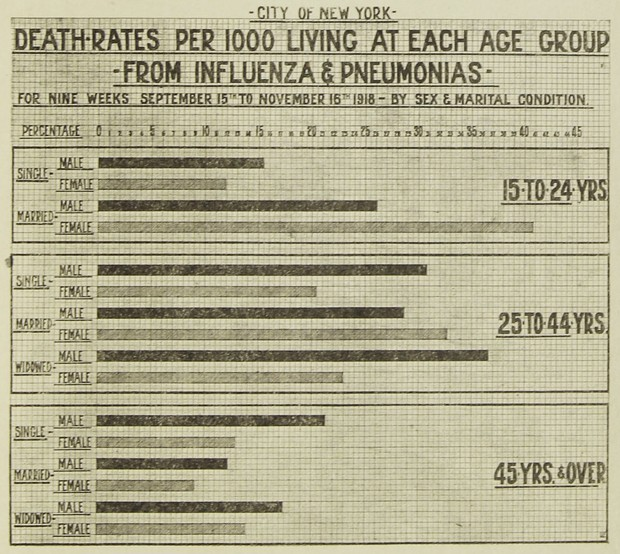
\includegraphics{figures/influenza_1918_new_york.jpg}

But disregarding the time investment: This is data science. You collect data (in this case, Influenza mortality), look for patterns and try to find underlying mechanisms that may explain the patterns (Age, Gender, Marital Status).

(\href{https://www.nytimes.com/2020/04/02/nyregion/spanish-flu-nyc-virus.html}{source})

\hypertarget{why-do-statistical-programming}{%
\section{Why do statistical programming?}\label{why-do-statistical-programming}}

Since you're a life science student -that is my target audience at least-, you have probably worked with Excel or SPSS at some time. Have you ever wondered

\begin{itemize}
\tightlist
\item
  Why am I doing this exact same series of mouse clicks again and again? Is there not a more efficient way?
\item
  How can I describe my work reproducible as a series of mouse clicks?
\end{itemize}

If so, then R may be your next favorite data analysis tool.
It takes a little effort at first, but once you get the hang of it you will never create a plot in Excel again.

With R - as with any programming language,

\begin{itemize}
\tightlist
\item
  Redoing an analysis or generating a report with minor adjustments is a breeze
\item
  The analysis is central, not the output. This guarantees complete reproducibility
\end{itemize}

\hypertarget{overview-of-the-toolbox}{%
\subsection*{Overview of the toolbox}\label{overview-of-the-toolbox}}
\addcontentsline{toc}{subsection}{Overview of the toolbox}

This chapter will introduce you to a toolbox that will serve you well during your data quests.\\
It consists of

\begin{itemize}
\tightlist
\item
  The R programming language and built-in functionality
\item
  The RStudio Integrated Development Environment (IDE)
\item
  R Markdown as documenting and reporting tool
\end{itemize}

\hypertarget{tool-1-the-r-programming-language}{%
\section{Tool 1: The R programming language}\label{tool-1-the-r-programming-language}}


\includegraphics{figures/Rlogo.jpg}

Nobody likes to pay for computer tools. R is completely free of charge. Moreover, it is completely open source. This is of course one of the main reasons for its popularity; other statistical tools are not free and sometimes downright expensive.
Besides this free nature, R is very popular because it has an interactive mode. We call this a read--evaluate--print loop: REPL. This means you don't need to write programs to run code. You simply type a command in the \textbf{\emph{console}}, press enter and immediately get the result on the line below.\\
As stated above, because you store your analyses in code, repeating these analyses -possibly with with new data or changed settings- is very easy.
One of my personal favorite features is that R supports ``literate programming'' for creating presentations (such as this one!) and other publications (reports, papers etc). Pdf documents, Microsoft Word documents, web pages (html) and e-books are all possible outputs of a single R Markdown master document.

Finally, R has advanced embedded graphical support. This means that graphical output (a plot) is as easy to generate as textual output!

Here are some figures to whet your appetite. You will be able to create all of these yourself at the end of this course (actually, a pair of courses).

\begin{figure}

{\centering 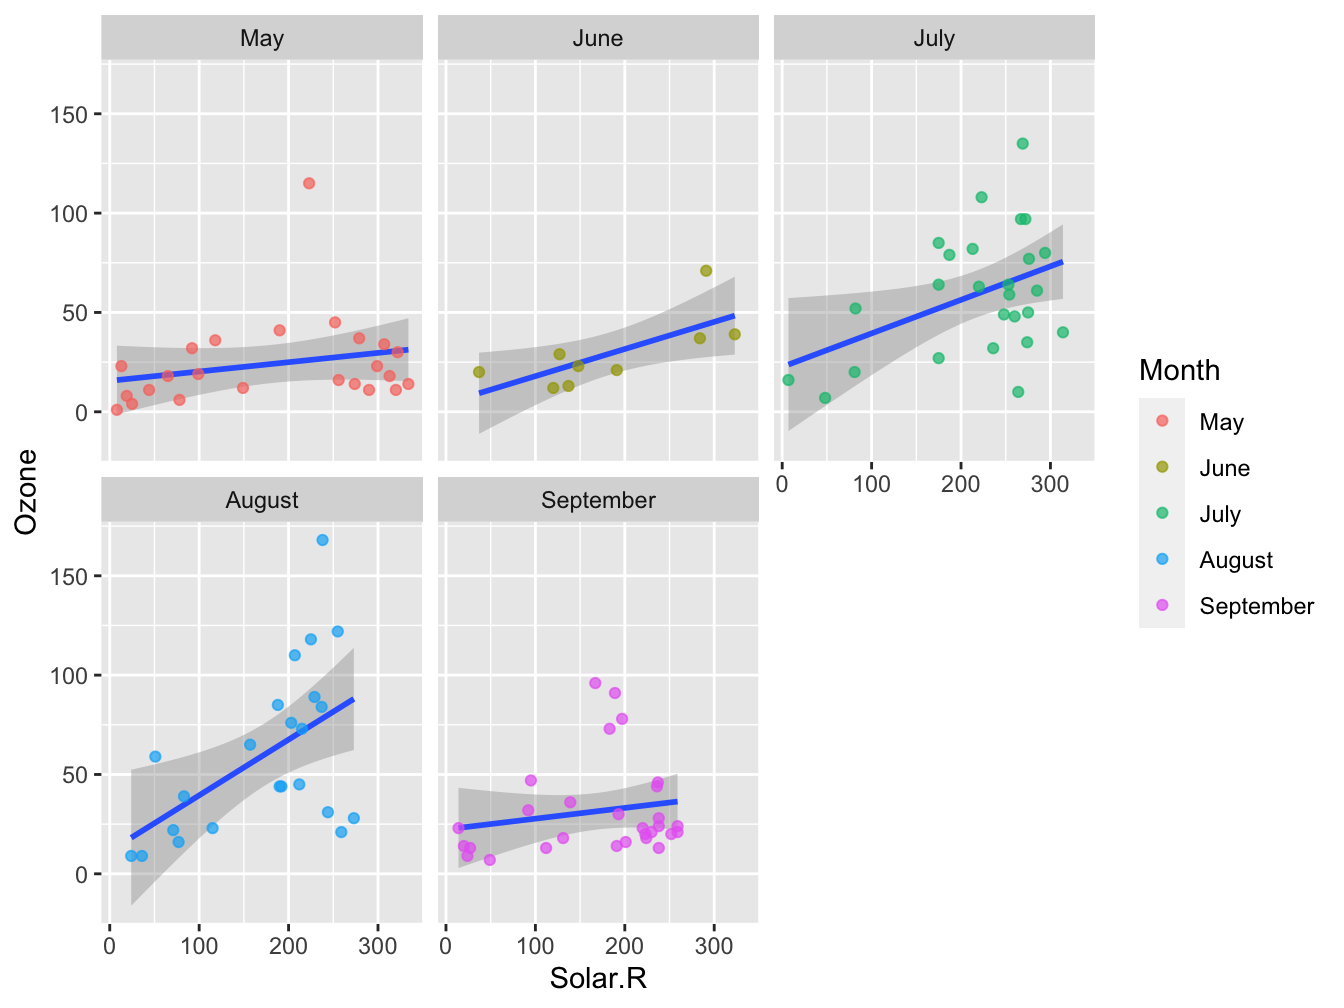
\includegraphics[width=0.8\linewidth]{davur_ebook_files/figure-latex/facetting-example-1} 

}

\caption{A facetplot - multiple similar plots split over a single nominal or ordinal variable}\label{fig:facetting-example}
\end{figure}

\begin{figure}

{\centering 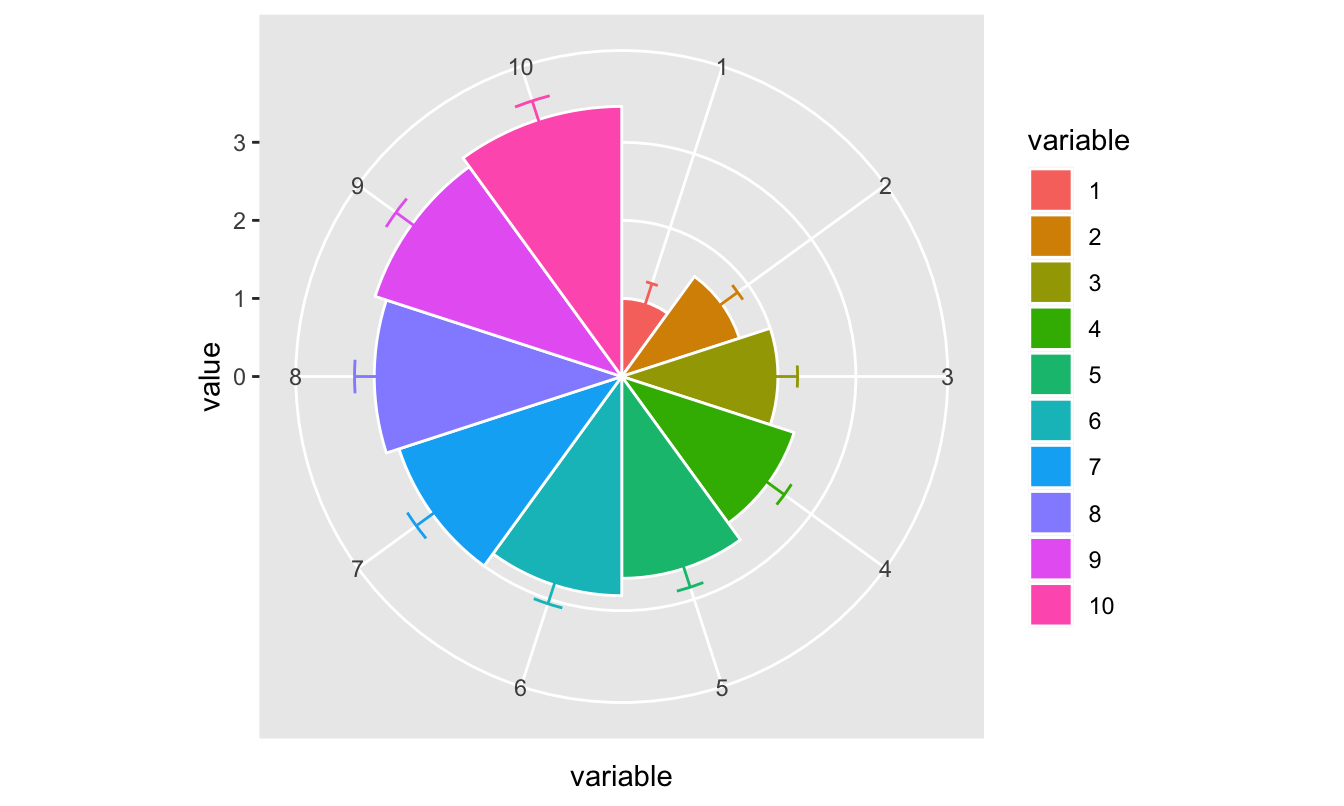
\includegraphics[width=0.8\linewidth]{davur_ebook_files/figure-latex/polarplot-1} 

}

\caption{A polar plot - the dimensions are not your normal 2d x and y}\label{fig:polarplot}
\end{figure}

\begin{figure}
\centering
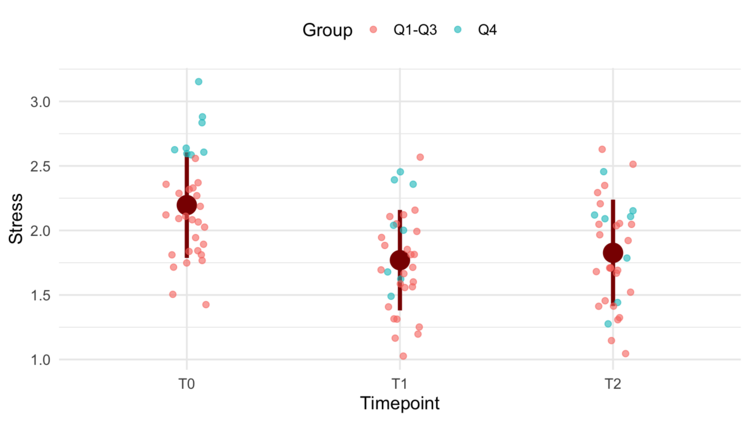
\includegraphics{figures/ptsd-jitter-5-1s.png}
\caption{A custom jitter visualization}
\end{figure}

\hypertarget{tool-2-rstudio-as-development-environment}{%
\section{Tool 2: RStudio as development environment}\label{tool-2-rstudio-as-development-environment}}

\begin{figure}
\centering

\includegraphics{figures/RStudioLogo.png}
\caption{RStudio logo}
\end{figure}

RStudio is a so-called Integrated Development Environment. This means it is a ``Swiss Multitool'' for programming. With it, you manage and run code, files, documentation on the language (help pages), building different output formats.
The workbench has several panels and looks like this when you run the application.

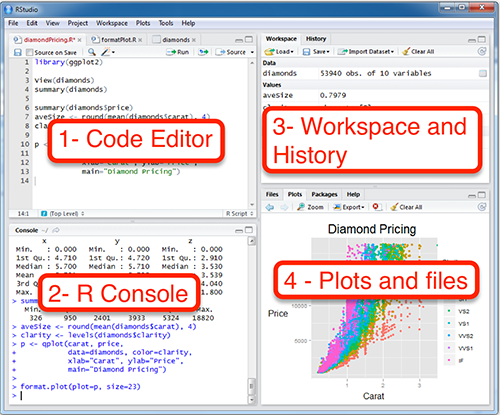
\includegraphics{figures/RStudio_screen3.png}

You primarily work with 4 panels of the workbench:

\begin{enumerate}
\def\labelenumi{\arabic{enumi}.}
\tightlist
\item
  \textbf{Code editor} where you write your scripts and R Markdown documents: text files with code you want to execute more than once
\item
  \textbf{R console} where you execute lines of code one by one
\item
  \textbf{Environment and History} See what data you have in memory, and what you have done so far
\item
  \textbf{Plots, Help \& Files}
\end{enumerate}

You use the console to do basic calculations, try pieces of code, develop a function, or load scripts (from the code editor) into memory. On the other hand, the code editor is used to work on code that has life span longer than a few minutes: analyses you may want to repeat, or develop further in the form of scripts and R Markdown documents.
The code editor supports many file types for viewing and editing: regular text, structured datafiles (text, csv, data files), scripts (programs), and analytical notebooks (R Markdown).

What is nice about the \textbf{\emph{code editor}} above regular text editors such as Notepad, Wordpad, TextEdit, is that it knows about different file types and their constituting elements and helps your read, write (auto-complete, error alerts), scan and organize them by displaying these elements using coloring, font types and other visual aids.

Here is the same piece of code, which is a plain text file, in two different editors. First as plain text in the Mac TextEdit app and next in the RStudio code editor:

\begin{figure}
\centering
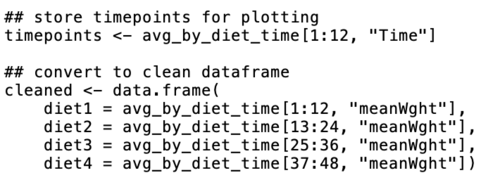
\includegraphics{figures/R_code_plain.png}
\caption{code in TextEdit}
\end{figure}

\begin{figure}
\centering
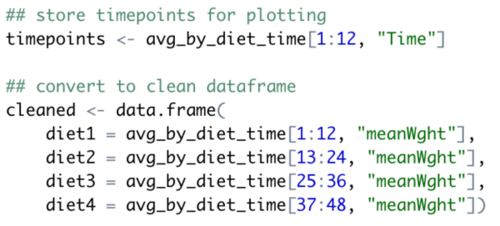
\includegraphics{figures/R_code_highlighted.png}
\caption{exact same file in RStudio editor}
\end{figure}

It is clearly visible where the code elements, numeric data and character data are within the code.

\hypertarget{tool-3-r-markdown}{%
\section{Tool 3: R Markdown}\label{tool-3-r-markdown}}


\includegraphics{figures/markdown_logo.jpg}

Using R Markdown you can combine regular text and figures with embedded R code that will be executed to generate a final document. We call this \emph{literate programming}.\\
You can use it to create reports in word, pdf or web (html), presentations (pdf or web) and even eBooks and websites. This entire eBook itself is written in R Markdown!

Markdown is, just like the language for the web, \texttt{html}, a \textbf{\emph{markup}} language. Markup means that you use textual elements to indicate structure instead of content. The R extension to Markdown, R Markdown, simply is Markdown with embedded pieces of R code. Consider this piece of Markdown:

\begin{verbatim}
## Tool 3: R Markdown

![](figures/markdown_logo.jpg)

Using RMarkdown you can combine regular text and figures with embedded R code that will be executed to generate a final document. 
\end{verbatim}

The result of this snippet, after it is converted into html, is the top of the current paragraph you are reading.

Here is a piece of R code we call a \textbf{\emph{code chunk}} that plots some random data in a scatter plot. In RStudio this piece of R code within (the current) R Markdown document looks like this:

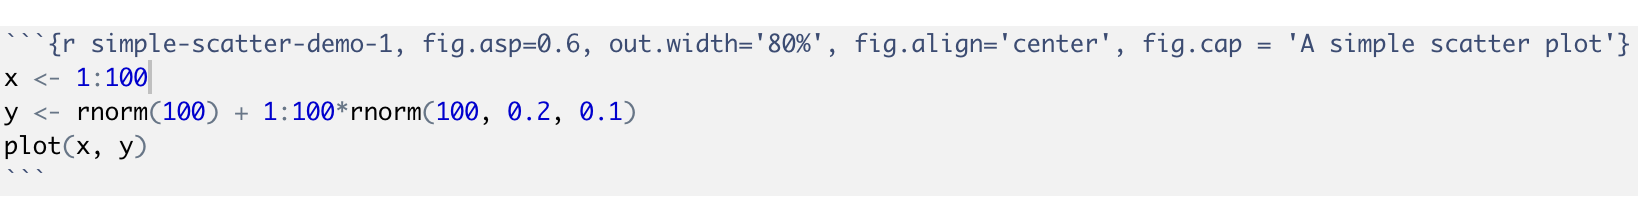
\includegraphics{figures/code_chunk.png}
Every code chunk consists of two parts; its \emph{header} and \emph{body}. The header tells the conversion engine (\textbf{\emph{knitr}}) how to deal with the code within the chunk, and its output.
In this case, this header is

\texttt{\{r\ simple-scatter-demo-1,\ fig.asp=0.6,\ out.width=\textquotesingle{}80\%\textquotesingle{},\ fig.align=\textquotesingle{}center\textquotesingle{},\ fig.caption=\textquotesingle{}A\ simple\ scatter\ plot\textquotesingle{}\}}

This header specifies quite a few things. First, the programming language (\texttt{r}) and the label, or ``name'', of the chunk (\texttt{simple-scatter-demo-1}). Next, several aspects of the generated plot are specified: its \emph{aspect ratio}, \emph{relative width}, \emph{alignment} on the page and the \emph{figure caption}. Only the programming language is required here.

Next, when you \textbf{\emph{knit}} (translate) the document into web format it results in the piece below, together with its output, a scatter plot.

\begin{Shaded}
\begin{Highlighting}[]
\NormalTok{x <-}\StringTok{ }\DecValTok{1}\OperatorTok{:}\DecValTok{100}
\NormalTok{y <-}\StringTok{ }\KeywordTok{rnorm}\NormalTok{(}\DecValTok{100}\NormalTok{) }\OperatorTok{+}\StringTok{ }\DecValTok{1}\OperatorTok{:}\DecValTok{100}\OperatorTok{*}\KeywordTok{rnorm}\NormalTok{(}\DecValTok{100}\NormalTok{, }\FloatTok{0.2}\NormalTok{, }\FloatTok{0.1}\NormalTok{)}
\KeywordTok{plot}\NormalTok{(x, y)}
\end{Highlighting}
\end{Shaded}

\begin{figure}

{\centering 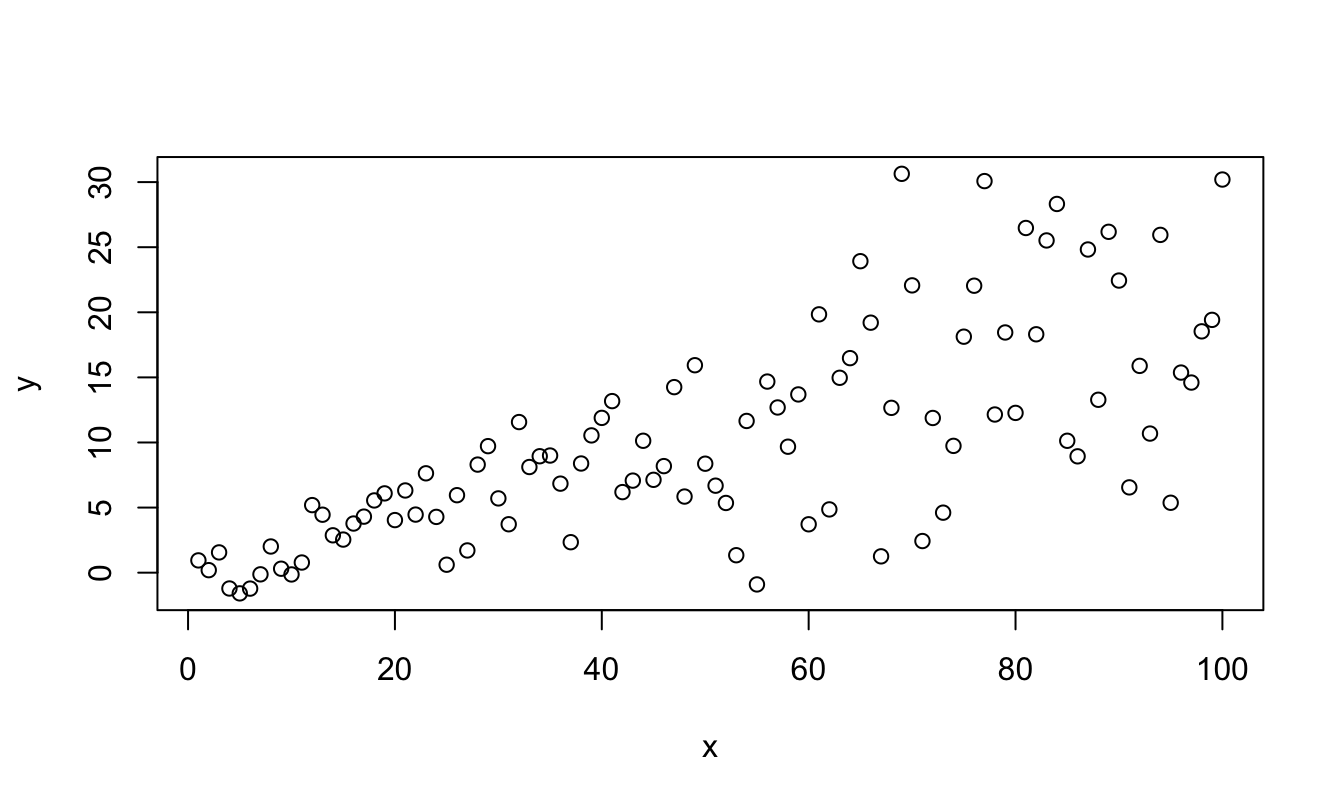
\includegraphics[width=0.8\linewidth]{davur_ebook_files/figure-latex/simple-scatter-demo-1-1} 

}

\caption{A simple scatter plot}\label{fig:simple-scatter-demo-1}
\end{figure}

R Markdown is translated into html, the markup language of the web, before any further processing occurs. That is why you can also embed html code elements within it but that is outside the scope of this course.\\
Here are the most basic elements you can use in Markdown documents.

\begin{figure}
\centering
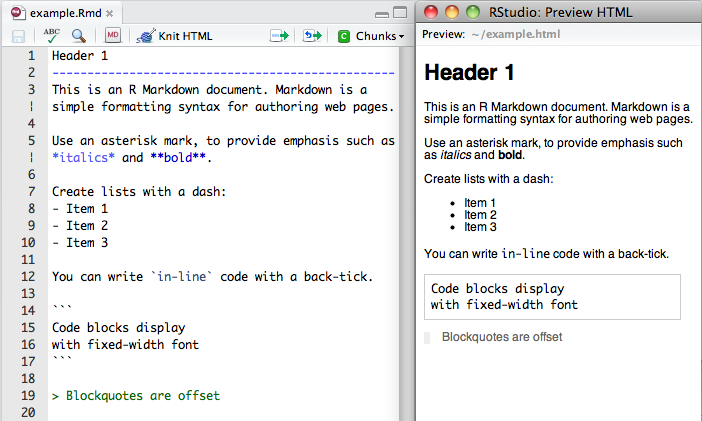
\includegraphics{figures/markdownOverview.png}
\caption{RMarkdown}
\end{figure}

Finally, it is also possible to embed Latex elements. For instance, equations can be defined in a text format. This:

\begin{verbatim}
$$d(p, q) = \sqrt{\sum_{i = 1}^{n}(q_i-p_i)^2}$$
\end{verbatim}

results in this:

\[d(p, q) = \sqrt{\sum_{i = 1}^{n}(q_i-p_i)^2}\]

RStudio provides several cheatsheets with R, including Markdown. Have a look at Help → Cheatsheets.

A final note. To be able to convert R Markdown into Word format you need to have MS Word installed on that machine. If you want to be able to generate pdf documents, you will need a bit more: see the screencast \href{https://www.youtube.com/watch?v=YL3avjNu6Ak}{Setting up on a Windows system}. It is a bit outdated so you should update to more recent version numbers.

\hypertarget{resources}{%
\section{Resources}\label{resources}}

\hypertarget{swirl-course}{%
\subsection*{Swirl course}\label{swirl-course}}
\addcontentsline{toc}{subsection}{Swirl course}

Swirl course to accompany this course: \url{http://github.com/MichielNoback/R_Data_Analysis}

\hypertarget{data-files}{%
\subsection*{Data Files}\label{data-files}}
\addcontentsline{toc}{subsection}{Data Files}

In this section all data files used or required for the course presentations or exercises are listed.\\

Whale selenium data:
whale\_selenium.txt

Bird observation data:
Observations-Data-2014.xlsx or, as
csv

Food constituents:
food\_constituents.txt

Wine review data:
winemag-data-130k-v2.csv

\hypertarget{web-resources-and-references}{%
\subsection*{Web resources and references}\label{web-resources-and-references}}
\addcontentsline{toc}{subsection}{Web resources and references}

\begin{itemize}
\item
  \textbf{R Markdown}\\
  R Markdown is a Markdown ``Dialect'' used for presenting, documenting and reporting in R: \href{http://rmarkdown.rstudio.com/}{http://rmarkdown.rstudio.com}
\item
  \textbf{R cheat sheet}\\
  The \href{figures/R_cheatsheet.pdf}{R cheat sheet}.
\item
  \textbf{R Markdown reference}\\
  The \href{https://www.rstudio.com/wp-content/uploads/2015/03/rmarkdown-reference.pdf}{RMarkdown reference} cards with extensive documentation. Also available at the computer exam!
\item
  \textbf{Bioconductor}\\
  Bioconductor provides tools for the analysis and comprehension of high- throughput genomic data: \href{http://www.bioconductor.org/}{http://www.bioconductor.org}
\end{itemize}

\hypertarget{screencasts}{%
\subsubsection*{Screencasts}\label{screencasts}}
\addcontentsline{toc}{subsubsection}{Screencasts}

Setting up on a Windows system
YouTube

Starting with R studio
YouTube

\hypertarget{basic-r---coding-basics}{%
\chapter{Basic R - coding basics}\label{basic-r---coding-basics}}

\hypertarget{first-look-at-vectors-fuctions-and-variables}{%
\section{First look at vectors, fuctions and variables}\label{first-look-at-vectors-fuctions-and-variables}}

\hypertarget{doing-math-in-the-console}{%
\subsection{Doing Math in the console}\label{doing-math-in-the-console}}

The console is the place where you do quick calculations, tests and analyses that do not need to be saved (yet) or repeated. It is the the tab that says ``Console'' and on first use, R puts it in the lower left panel.

In the console, the \textbf{\emph{prompt}} is the ``greater than'' symbol ``\textgreater{}''. R waits here for you to enter commands. When the panel has ``focus'' the cursor is blinking on and off. You can use the console as a calculator. It supports all regular math operations, in the way you would expect them:

\texttt{+}  : `plus', as in 2 + 2 = 4

\texttt{-} : `subtract', as in 2 - 2 = 0

\texttt{*}  : `multiply', as in 2 * 3 = 6

\texttt{/}  : `divide', as in 8 / 4 = 2

\texttt{\^{}}  : `exponent', as in 2\^{}3 = 8. In R, \texttt{\^{}} is synonym of \texttt{**}

For the square root you can use \(n^{0.5}\): \texttt{n**0.5}, or the function \texttt{sqrt()} (discussed later).

When Enter is pressed when the mathematical statement is not complete yet, the \texttt{\textgreater{}} symbol is replaced by a \texttt{+} at the start of the new line, indicating the statement is a continuation. Here is an example:

\begin{verbatim}
> 1 + 3 + 4 + 
+ 
\end{verbatim}

So the \texttt{+} at the start of line 2 is not a mathematical \texttt{+} but a ``continuation symbol''. You can always abort the current statement by pressing Escape.

When a statement \emph{is} complete, the result will be printed in the next line:

\begin{verbatim}
> 31 + 11
[1] 42
\end{verbatim}

The result is of course \texttt{42}; the leading \texttt{{[}1{]}} is the \textbf{\emph{index}} of the result. We will address this later.

\hypertarget{operator-precedence}{%
\subsubsection*{Operator Precedence}\label{operator-precedence}}
\addcontentsline{toc}{subsubsection}{Operator Precedence}

All ``operators'' adhere to the standard mathematical \textbf{precedence} rules (PEMDAS):

\begin{verbatim}
    Parentheses (simplify inside these)
    Exponents
    Multiplication and Division (from left to right)
    Addition and Subtraction (from left to right)
\end{verbatim}

With complex statements you should be aware of operator precedence! If you are not sure, or want to make your expression less ambiguous you should simply use parentheses \texttt{()} because they have highest precedence.

Besides math operators, R knows a whole set of other operators. They will be dealt with later in this chapter.

\begin{quote}
\textbf{\emph{Programming Rule}} Always place spaces around both sides of an operator, with the exception of \texttt{\^{}} and \texttt{**}.
\end{quote}

\hypertarget{an-expression-dissected}{%
\subsection{An expression dissected}\label{an-expression-dissected}}

When you type \texttt{21\ /\ 3} this called an \textbf{\emph{expression}}. The expression has three parts: an operator (\texttt{/} in the middle) and two operands. The left operand is \texttt{21} and the right operand is \texttt{3}.\\
Since there is no assignment, the result of this expression will be send to the console as output, giving \texttt{{[}1{]}\ 7}.

Because this expression is the sole contents of the current line in the console, it is also called a \textbf{\emph{statement}}.

\begin{quote}
\textbf{\emph{Statement vs expression}} A statement is a complete line of code that performs some action, while an expression is any section of code that evaluates to a value.
\end{quote}

\hypertarget{ending-statements}{%
\subsubsection*{Ending statements}\label{ending-statements}}
\addcontentsline{toc}{subsubsection}{Ending statements}

In R, the newline (enter) is an end-of-statement character. Optionally you can end statements with a semicolon ``;''. However, when you have more statements on a single line they are mandatory is in this example:

\begin{Shaded}
\begin{Highlighting}[]
\NormalTok{x <-}\StringTok{ }\KeywordTok{c}\NormalTok{(}\DecValTok{1}\NormalTok{, }\DecValTok{2}\NormalTok{, }\DecValTok{3}\NormalTok{); x; x <-}\StringTok{ }\DecValTok{42}\NormalTok{; x}
\end{Highlighting}
\end{Shaded}

\begin{verbatim}
## [1] 1 2 3
\end{verbatim}

\begin{verbatim}
## [1] 42
\end{verbatim}

\begin{quote}
\textbf{\emph{Programming Rule}}: Have one statement per line and don't use semicolons
\end{quote}

\hypertarget{comments}{%
\subsubsection*{Comments}\label{comments}}
\addcontentsline{toc}{subsubsection}{Comments}

Everything on a line after a hash sign ``\texttt{\#}'' will be ignored by R. Use it to add explanation to your code:

\begin{Shaded}
\begin{Highlighting}[]
\CommentTok{## starting cool analysis}
\NormalTok{x <-}\StringTok{ }\KeywordTok{c}\NormalTok{(T, F, T) }\CommentTok{# Creating a logical vector}
\NormalTok{y <-}\StringTok{ }\KeywordTok{c}\NormalTok{(}\OtherTok{TRUE}\NormalTok{, }\OtherTok{FALSE}\NormalTok{, }\OtherTok{TRUE}\NormalTok{) }\CommentTok{# same}
\end{Highlighting}
\end{Shaded}

\hypertarget{functions}{%
\section{Functions}\label{functions}}

Simple mathematics is not the core business of R.

Going further than basic math, you will need functions, mostly pre-existing functions but often also custom functions that you write yourself. Here is a definition of a function:

\begin{quote}
\emph{A function is a piece of functionality that you can execute by typing its name, followed by a pair of parentheses. Within these parentheses, you can pass data for the function to work on. Functions often, but not always, return a value}.
\end{quote}

Function usage -or a \textbf{\emph{function call}}- has this general form:
\[function\_name(arg_1, arg_2, ..., arg_n)\]

\hypertarget{example-square-root-with-sqrt}{%
\subsubsection*{\texorpdfstring{Example: Square root with \texttt{sqrt()}}{Example: Square root with sqrt()}}\label{example-square-root-with-sqrt}}
\addcontentsline{toc}{subsubsection}{Example: Square root with \texttt{sqrt()}}

You have already seen that the square root can be calculated as \(n^{0.5}\).
However, there is also a function for it: \texttt{sqrt()}. It \textbf{\emph{returns}} the square root of the given \textbf{\emph{parameter}}, a number, \emph{e.g.} \texttt{sqrt(36)}

\begin{Shaded}
\begin{Highlighting}[]
\DecValTok{36}\OperatorTok{^}\FloatTok{0.5}
\KeywordTok{sqrt}\NormalTok{(}\DecValTok{36}\NormalTok{)}
\end{Highlighting}
\end{Shaded}

\begin{verbatim}
## [1] 6
## [1] 6
\end{verbatim}

\hypertarget{another-example-paste}{%
\subsubsection*{\texorpdfstring{Another example: \texttt{paste()}}{Another example: paste()}}\label{another-example-paste}}
\addcontentsline{toc}{subsubsection}{Another example: \texttt{paste()}}

The \texttt{paste()} function can take any number of arguments and returns them, combined into a single text (character) string. You can also specify a separator using \texttt{sep="\textless{}separator\ string\textgreater{}"}:

\begin{Shaded}
\begin{Highlighting}[]
\KeywordTok{paste}\NormalTok{(}\DecValTok{1}\NormalTok{, }\DecValTok{2}\NormalTok{, }\DecValTok{3}\NormalTok{, }\DataTypeTok{sep =} \StringTok{"---"}\NormalTok{)}
\end{Highlighting}
\end{Shaded}

\begin{verbatim}
## [1] "1---2---3"
\end{verbatim}

Note the use of quotes surrounding the dashes: \texttt{"-\/-\/-"}; they indicate it is text, or character, data.\\
Also note the use of a name for only the last argument. Not all arguments can be specified by name, but when possible this has preference, as in \texttt{sep\ =\ "-\/-\/-"}.

\hypertarget{getting-help-on-a-function}{%
\subsection{Getting help on a function}\label{getting-help-on-a-function}}

Type \texttt{?function\_name} or \texttt{help(function\_name)} in the console to get help on a function. The function documentation will appear in the panel containing the \texttt{Help} tab, Its location is dependent on your set of preferences.\\
For instance, typing \texttt{?sqrt} will give the help page of the square root function together with the \texttt{abs()} function.\\
R help pages always have the exact same structure:

\begin{itemize}
\tightlist
\item
  Name \& package (e.g. \texttt{\{base\}})
\item
  Short description
\item
  Description
\item
  Usage
\item
  Arguments
\item
  Details
\item
  \ldots{}
\item
  Examples
\end{itemize}

Scroll down in the help to see example usages of the function. Alternatively, type \texttt{example(sqrt)} in the console to have all examples executed in order, until you press Escape.

\hypertarget{variables}{%
\section{Variables}\label{variables}}

In math and programming you often use variables to label or name pieces of data, or a function in order to have them reusable, retrievable, changeable.

\begin{quote}
A \textbf{\emph{variable}} is a named piece of data stored in memory that can be accessed via its name
\end{quote}

For instance, \texttt{x\ =\ 42} is used to define a variable called \texttt{x}, with a value attached to it of \texttt{42}. Variables are really \emph{variable} - their value can change!
In R you usually assign a value to a variable using ``\texttt{\textless{}-}'', so ``\texttt{x\ \textless{}-\ 42}'' is equivalent to ``\texttt{x\ =\ 42}''. Both will work in R, but the ``arrow'' notation is preferred.

\hypertarget{vectors}{%
\section{Vectors}\label{vectors}}

\hypertarget{r-is-completely-vector-based}{%
\subsection{R is completely vector-based}\label{r-is-completely-vector-based}}

In R, \emph{\textbf{all data lives inside vectors}}. When you type `2 + 4', R will execute the following series of actions:

\begin{enumerate}
\def\labelenumi{\arabic{enumi}.}
\tightlist
\item
  create a vector of length 1 with its element having the value 2
\item
  create a vector of length 1 with its element having the value 4
\item
  add the value of the second vector to ALL the values of vector one, and recycle any shorter vector as many times as needed
\end{enumerate}

Step 3 is a crucial one. It is essential to grasp this aspect in order to understand R. Therefore we'll revisit it later in more detail.

\hypertarget{five-datatype-that-live-in-vectors}{%
\subsection{Five datatype that live in vectors}\label{five-datatype-that-live-in-vectors}}

R knows five basic types of data:

\begin{tabular}{l|l|l}
\hline
type & descripton & examples\\
\hline
numeric & numbers with a decimal part & `3.123`, `5000.0`, `4.1E3`\\
\hline
integer & numbers without a decimal part & `1`, `0`, `2999`\\
\hline
logical & Boolean values: yes/no) & `true` `false`\\
\hline
character & text, should be put within quotes & `'hello R'` `"A cat!"`\\
\hline
factor & nominal and ordinal scales & \textbackslash{}<dealt with later\textbackslash{}>\\
\hline
\end{tabular}

All these types are created in similar ways and can often be converted into other types.

\textbf{Note 1:} If you type a number in the console, it will always be a \texttt{numeric} value, decimal part or not.\\
\textbf{Note 2:} For character data, single and double quotes are equivalent but double are preferred; type \texttt{?Quotes} in the console to read more on this topic.

\hypertarget{creating-vectors}{%
\subsection{Creating vectors}\label{creating-vectors}}

You will see shortly that there are many ways to create vectors: a custom collection, a series, a repetition of a smaller set, a random sample from a distribution, etc. etc.

The simplest way to create a vector is the first: create a vector from a custom set of elements, using the ``Concatenate'' function \texttt{c()}. The \texttt{c()} function simply takes all its arguments and puts them behind each other, in the order in which they were passed to it, and returns the resulting vector.

\begin{Shaded}
\begin{Highlighting}[]
\OperatorTok{>}\StringTok{ }\KeywordTok{c}\NormalTok{(}\DecValTok{2}\NormalTok{, }\DecValTok{4}\NormalTok{, }\DecValTok{3}\NormalTok{)}
\end{Highlighting}
\end{Shaded}

\begin{verbatim}
## [1] 2 4 3
\end{verbatim}

\begin{Shaded}
\begin{Highlighting}[]
\OperatorTok{>}\StringTok{ }\KeywordTok{c}\NormalTok{(}\StringTok{"a"}\NormalTok{, }\StringTok{"b"}\NormalTok{, }\KeywordTok{c}\NormalTok{(}\StringTok{"c"}\NormalTok{, }\StringTok{"d"}\NormalTok{))}
\end{Highlighting}
\end{Shaded}

\begin{verbatim}
## [1] "a" "b" "c" "d"
\end{verbatim}

\begin{Shaded}
\begin{Highlighting}[]
\OperatorTok{>}\StringTok{ }\KeywordTok{c}\NormalTok{(}\FloatTok{0.1}\NormalTok{, }\FloatTok{0.01}\NormalTok{, }\FloatTok{0.001}\NormalTok{)}
\end{Highlighting}
\end{Shaded}

\begin{verbatim}
## [1] 0.100 0.010 0.001
\end{verbatim}

\begin{Shaded}
\begin{Highlighting}[]
\OperatorTok{>}\StringTok{ }\KeywordTok{c}\NormalTok{(T, F, }\OtherTok{TRUE}\NormalTok{, }\OtherTok{FALSE}\NormalTok{) }\CommentTok{# There are two way to write logical values}
\end{Highlighting}
\end{Shaded}

\begin{verbatim}
## [1]  TRUE FALSE  TRUE FALSE
\end{verbatim}

\hypertarget{vectors-can-hold-only-one-data-type}{%
\subsubsection*{Vectors can hold only one data type}\label{vectors-can-hold-only-one-data-type}}
\addcontentsline{toc}{subsubsection}{Vectors can hold only one data type}

A vector can hold only one type of data. Therefore, if you pass a mixed set of values to the function \texttt{c()}, it will \textbf{coerce} all data into one type. The preferred type is numeric. However, when that is not possible the result will most often be a character vector. In the example below, two numbers and a character value are passed. Since \texttt{"a"} cannot be coerced into a numeric, the returned vector will be a character vector.

\begin{Shaded}
\begin{Highlighting}[]
\KeywordTok{c}\NormalTok{(}\DecValTok{2}\NormalTok{, }\DecValTok{4}\NormalTok{, }\StringTok{"a"}\NormalTok{) }
\end{Highlighting}
\end{Shaded}

\begin{verbatim}
## [1] "2" "4" "a"
\end{verbatim}

Here are some more coercion examples.

\begin{Shaded}
\begin{Highlighting}[]
\OperatorTok{>}\StringTok{ }\KeywordTok{c}\NormalTok{(}\DecValTok{1}\NormalTok{, }\DecValTok{2}\NormalTok{, }\OtherTok{TRUE}\NormalTok{) }\CommentTok{# To numeric}
\end{Highlighting}
\end{Shaded}

\begin{verbatim}
## [1] 1 2 1
\end{verbatim}

\begin{Shaded}
\begin{Highlighting}[]
\OperatorTok{>}\StringTok{ }\KeywordTok{c}\NormalTok{(}\OtherTok{TRUE}\NormalTok{, }\OtherTok{FALSE}\NormalTok{, }\StringTok{"TRUE"}\NormalTok{) }\CommentTok{# To character}
\end{Highlighting}
\end{Shaded}

\begin{verbatim}
## [1] "TRUE"  "FALSE" "TRUE"
\end{verbatim}

\begin{Shaded}
\begin{Highlighting}[]
\OperatorTok{>}\StringTok{ }\KeywordTok{c}\NormalTok{(}\FloatTok{1.3}\NormalTok{, }\OtherTok{TRUE}\NormalTok{, }\StringTok{"1"}\NormalTok{) }\CommentTok{# To character}
\end{Highlighting}
\end{Shaded}

\begin{verbatim}
## [1] "1.3"  "TRUE" "1"
\end{verbatim}

Using the function \texttt{class()}, you can get the data type of any value or variable.

\begin{Shaded}
\begin{Highlighting}[]
\OperatorTok{>}\StringTok{ }\KeywordTok{class}\NormalTok{(}\KeywordTok{c}\NormalTok{(}\DecValTok{2}\NormalTok{, }\DecValTok{4}\NormalTok{, }\StringTok{"a"}\NormalTok{))}
\end{Highlighting}
\end{Shaded}

\begin{verbatim}
## [1] "character"
\end{verbatim}

\begin{Shaded}
\begin{Highlighting}[]
\OperatorTok{>}\StringTok{ }\KeywordTok{class}\NormalTok{(}\DecValTok{1}\OperatorTok{:}\DecValTok{5}\NormalTok{)}
\end{Highlighting}
\end{Shaded}

\begin{verbatim}
## [1] "integer"
\end{verbatim}

\begin{Shaded}
\begin{Highlighting}[]
\OperatorTok{>}\StringTok{ }\KeywordTok{class}\NormalTok{(}\KeywordTok{c}\NormalTok{(}\DecValTok{2}\NormalTok{, }\DecValTok{4}\NormalTok{, }\FloatTok{0.3}\NormalTok{))}
\end{Highlighting}
\end{Shaded}

\begin{verbatim}
## [1] "numeric"
\end{verbatim}

\begin{Shaded}
\begin{Highlighting}[]
\OperatorTok{>}\StringTok{ }\KeywordTok{class}\NormalTok{(}\KeywordTok{c}\NormalTok{(}\DecValTok{2}\NormalTok{, }\DecValTok{4}\NormalTok{, }\DecValTok{3}\NormalTok{))}
\end{Highlighting}
\end{Shaded}

\begin{verbatim}
## [1] "numeric"
\end{verbatim}

\hypertarget{vector-fiddling}{%
\subsection{Vector fiddling}\label{vector-fiddling}}

\hypertarget{vector-arithmetic}{%
\subsubsection*{Vector arithmetic}\label{vector-arithmetic}}
\addcontentsline{toc}{subsubsection}{Vector arithmetic}

Let's have a look at what it means to work with vectors, as opposed to singular values (also called \emph{scalars}). An example is probably best to get an idea.

\begin{Shaded}
\begin{Highlighting}[]
\NormalTok{x <-}\StringTok{ }\KeywordTok{c}\NormalTok{(}\DecValTok{2}\NormalTok{, }\DecValTok{4}\NormalTok{, }\DecValTok{3}\NormalTok{, }\DecValTok{5}\NormalTok{)}
\NormalTok{y <-}\StringTok{ }\KeywordTok{c}\NormalTok{(}\DecValTok{6}\NormalTok{, }\DecValTok{2}\NormalTok{)}
\NormalTok{x }\OperatorTok{+}\StringTok{ }\NormalTok{y}
\end{Highlighting}
\end{Shaded}

\begin{verbatim}
## [1] 8 6 9 7
\end{verbatim}

As you can see, R works \textbf{\emph{set based}} and will \textbf{\emph{cycle}} the shorter of the two operands to deal with all elements of the longer operand. How about when the longer one is not a multiple of the shorter one?

\begin{Shaded}
\begin{Highlighting}[]
\NormalTok{x <-}\StringTok{ }\KeywordTok{c}\NormalTok{(}\DecValTok{2}\NormalTok{, }\DecValTok{4}\NormalTok{, }\DecValTok{3}\NormalTok{, }\DecValTok{5}\NormalTok{)}
\NormalTok{z <-}\StringTok{ }\KeywordTok{c}\NormalTok{(}\DecValTok{1}\NormalTok{, }\DecValTok{2}\NormalTok{, }\DecValTok{3}\NormalTok{)}
\NormalTok{x }\OperatorTok{-}\StringTok{ }\NormalTok{z}
\end{Highlighting}
\end{Shaded}

\begin{verbatim}
## Warning in x - z: longer object length is not a multiple of shorter object
## length
\end{verbatim}

\begin{verbatim}
## [1] 1 2 0 4
\end{verbatim}

As you can see this generates a warning that ``longer object length is not a multiple of shorter object length''. However, R will proceed anyway, cycling the shorter one.

\hypertarget{other-operators}{%
\section{Other operators}\label{other-operators}}

Here is a complete listing of operators in R. Some operators such as \texttt{\^{}} are \emph{unary}, which means they have a single \emph{operand}; a single value or they operate on. On the other hand, \emph{binary} operators such as \texttt{+} have two \emph{operands}.

The following unary and binary operators are listed in precedence groups, from highest to lowest. Many of them are still unknown to you of course. We will encounter most of these along the way as the course progresses, starting with a few in this section.

\begin{tabular}{l|l}
\hline
operator & purpose\\
\hline
:: ::: & access variables in a namespace\\
\hline
\$ @ & component / slot extraction\\
\hline
[ [[ & indexing\\
\hline
\textasciicircum{} & exponentiation (right to left)\\
\hline
- + & unary minus and plus\\
\hline
: & sequence operator\\
\hline
\%any\% & special operators (including \%\% and \%/\%)\\
\hline
* / & multiply, divide\\
\hline
+ - & (binary) add, subtract\\
\hline
< > <= >= == != & ordering and comparison\\
\hline
! & negation\\
\hline
\& \&\& & and\\
\hline
| || & or\\
\hline
\textasciitilde{} & as in formulae\\
\hline
-> ->> & rightwards assignment\\
\hline
<- <<- & assignment (right to left)\\
\hline
= & assignment (right to left)\\
\hline
? & help (unary and binary)\\
\hline
\end{tabular}

\hypertarget{logical-operators}{%
\subsection{Logical operators}\label{logical-operators}}

Logical operators are used to evaluate and/or combine expressions that result in a single logical value: \texttt{TRUE} or \texttt{FALSE}. The \textbf{\emph{comparison operators}} compare two values (numeric, character - any type is possible) to get to a logical value, but always set-based! In the following chunk, each of the values in \texttt{x} is considered and if it is smaller than or equal to the value \texttt{4}, \texttt{TRUE} is returned, else \texttt{FALSE}.

\begin{Shaded}
\begin{Highlighting}[]
\NormalTok{x <-}\StringTok{ }\KeywordTok{c}\NormalTok{(}\DecValTok{1}\NormalTok{, }\DecValTok{5}\NormalTok{, }\DecValTok{4}\NormalTok{, }\DecValTok{3}\NormalTok{)}
\NormalTok{x }\OperatorTok{<=}\StringTok{ }\DecValTok{4}
\end{Highlighting}
\end{Shaded}

\begin{verbatim}
## [1]  TRUE FALSE  TRUE  TRUE
\end{verbatim}

Other comparison operators are \texttt{\textless{}} (less then), \texttt{\textless{}=} (less then or equal to), \texttt{\textgreater{}} (greater then), \texttt{\textgreater{}=} (greater then or equal to), and \texttt{==} (equal to).

Another category of logical operators is the set of \textbf{\emph{boolean operators}}. These are used to \emph{reduce} two logical values into one. These are

\begin{itemize}
\tightlist
\item
  \texttt{\&}: logical ``AND''; \texttt{a\ \&\ b} will evaluate to \texttt{TRUE} only if \texttt{a} AND \texttt{b} are TRUE.\\
\item
  \texttt{\textbar{}}: logical ``OR''; \texttt{a\ \textbar{}\ b} will evaluate to \texttt{TRUE} only if \texttt{a} OR \texttt{b} are TRUE, no matter which.
\item
  \texttt{!}: logical -unary- ``NOT''; negates the right operand: \texttt{!\ a} will evaluate to the ``flipped'' logical value of \texttt{a}.
\end{itemize}

Here is a more elaborate example combining comparison and boolean operators.
Suppose you have vectors a and b and you want to know which values in \texttt{a} are greater than in \texttt{b} and also smaller than \texttt{3}. This is the expression used for answering that question.

\begin{Shaded}
\begin{Highlighting}[]
\NormalTok{a <-}\StringTok{ }\KeywordTok{c}\NormalTok{(}\DecValTok{2}\NormalTok{, }\DecValTok{1}\NormalTok{, }\DecValTok{3}\NormalTok{, }\DecValTok{1}\NormalTok{, }\DecValTok{5}\NormalTok{, }\DecValTok{1}\NormalTok{)}
\NormalTok{b <-}\StringTok{ }\KeywordTok{c}\NormalTok{(}\DecValTok{1}\NormalTok{, }\DecValTok{2}\NormalTok{, }\DecValTok{4}\NormalTok{, }\DecValTok{2}\NormalTok{, }\DecValTok{3}\NormalTok{, }\DecValTok{0}\NormalTok{)}
\NormalTok{a }\OperatorTok{>}\StringTok{ }\NormalTok{b }\OperatorTok{&}\StringTok{ }\NormalTok{a }\OperatorTok{<}\StringTok{ }\DecValTok{3} \CommentTok{## returns a logical vector with test results}
\end{Highlighting}
\end{Shaded}

\begin{verbatim}
## [1]  TRUE FALSE FALSE FALSE FALSE  TRUE
\end{verbatim}

Here is a special case. Can you figure out what happens there?

\begin{Shaded}
\begin{Highlighting}[]
\DecValTok{6} \OperatorTok{-}\StringTok{ }\DecValTok{2} \OperatorTok{:}\StringTok{ }\DecValTok{5} \OperatorTok{<}\StringTok{ }\DecValTok{3}
\end{Highlighting}
\end{Shaded}

\begin{verbatim}
## [1] FALSE FALSE  TRUE  TRUE
\end{verbatim}

\hypertarget{calculations-with-logical-vectors}{%
\subsubsection*{Calculations with logical vectors}\label{calculations-with-logical-vectors}}
\addcontentsline{toc}{subsubsection}{Calculations with logical vectors}

Quite often you want to know how many cases fit some condition. A convenient thing in that case is that logical values have a numeric counterpart or ``hidden face'':

\begin{verbatim}
- TRUE == 1
- FALSE == 0
\end{verbatim}

\begin{itemize}
\tightlist
\item
  Use \texttt{sum()} to use this feature
\end{itemize}

\begin{Shaded}
\begin{Highlighting}[]
\NormalTok{x <-}\StringTok{ }\KeywordTok{c}\NormalTok{(}\DecValTok{2}\NormalTok{, }\DecValTok{4}\NormalTok{, }\DecValTok{2}\NormalTok{, }\DecValTok{1}\NormalTok{, }\DecValTok{5}\NormalTok{, }\DecValTok{3}\NormalTok{, }\DecValTok{6}\NormalTok{)}
\NormalTok{x }\OperatorTok{>}\StringTok{ }\DecValTok{3} \CommentTok{## which values are greater than 3?}
\end{Highlighting}
\end{Shaded}

\begin{verbatim}
## [1] FALSE  TRUE FALSE FALSE  TRUE FALSE  TRUE
\end{verbatim}

\begin{Shaded}
\begin{Highlighting}[]
\KeywordTok{sum}\NormalTok{(x }\OperatorTok{>}\StringTok{ }\DecValTok{3}\NormalTok{) }\CommentTok{## how many are greater than 3?}
\end{Highlighting}
\end{Shaded}

\begin{verbatim}
## [1] 3
\end{verbatim}

\hypertarget{modulo}{%
\subsection{\texorpdfstring{Modulo: \texttt{\%\%}}{Modulo: \%\%}}\label{modulo}}

The modulo operator gives the remainder of a division.

\begin{Shaded}
\begin{Highlighting}[]
\DecValTok{10} \OperatorTok\StringTok{ }\DecValTok{3}
\end{Highlighting}
\end{Shaded}

\begin{verbatim}
## [1] 1
\end{verbatim}

\begin{Shaded}
\begin{Highlighting}[]
\DecValTok{4} \OperatorTok\StringTok{ }\DecValTok{2}
\end{Highlighting}
\end{Shaded}

\begin{verbatim}
## [1] 0
\end{verbatim}

\begin{Shaded}
\begin{Highlighting}[]
\DecValTok{11} \OperatorTok\StringTok{ }\DecValTok{3}
\end{Highlighting}
\end{Shaded}

\begin{verbatim}
## [1] 2
\end{verbatim}

The modulo is most often used to establish periodicity: \texttt{x\ \%\%\ 2} is zero for all even numbers. Likewise, \texttt{x\ \%\%\ 10} will be zero for every tenth value.

\hypertarget{integer-division-and-rounding}{%
\subsection{\texorpdfstring{Integer division \texttt{\%/\%} and rounding}{Integer division \%/\% and rounding}}\label{integer-division-and-rounding}}

The integer division is the complement of modulo and gives the integer part of a division, it simply ``chops off'' the decimal part.

\begin{Shaded}
\begin{Highlighting}[]
\DecValTok{10} \OperatorTok\StringTok{ }\DecValTok{3}
\end{Highlighting}
\end{Shaded}

\begin{verbatim}
## [1] 3
\end{verbatim}

\begin{Shaded}
\begin{Highlighting}[]
\DecValTok{4} \OperatorTok\StringTok{ }\DecValTok{2}
\end{Highlighting}
\end{Shaded}

\begin{verbatim}
## [1] 2
\end{verbatim}

\begin{Shaded}
\begin{Highlighting}[]
\DecValTok{11} \OperatorTok\StringTok{ }\DecValTok{3}
\end{Highlighting}
\end{Shaded}

\begin{verbatim}
## [1] 3
\end{verbatim}

Note that \texttt{floor()} does the same. In the same manner, \texttt{ceiling()} rounds up to the nearest integer, no matter how large the decimal part. Finally, there is the \texttt{round()} method to be used for - well, rounding. Be aware that rounding in R is not the same as rounding your course grade which always goes up at \texttt{x.5}. Rounding \texttt{x.5} values mathematically goes to the nearest even number:

\begin{Shaded}
\begin{Highlighting}[]
\NormalTok{x <-}\StringTok{ }\KeywordTok{c}\NormalTok{(}\FloatTok{0.5}\NormalTok{, }\FloatTok{1.5}\NormalTok{, }\FloatTok{2.5}\NormalTok{, }\FloatTok{3.5}\NormalTok{, }\FloatTok{4.5}\NormalTok{, }\FloatTok{5.5}\NormalTok{, }\FloatTok{6.5}\NormalTok{, }\FloatTok{7.5}\NormalTok{)}
\KeywordTok{round}\NormalTok{(x, }\DecValTok{0}\NormalTok{)}
\end{Highlighting}
\end{Shaded}

\begin{verbatim}
## [1] 0 2 2 4 4 6 6 8
\end{verbatim}

\hypertarget{the-in-operator}{%
\subsection{\texorpdfstring{The \texttt{\%in\%} operator}{The \%in\% operator}}\label{the-in-operator}}

The \texttt{\%in\%} operator is very handy when you want to know if the elements of one vector are present in another vector. An example explains best, as usual:

\begin{Shaded}
\begin{Highlighting}[]
\NormalTok{a <-}\StringTok{ }\KeywordTok{c}\NormalTok{(}\StringTok{"one"}\NormalTok{, }\StringTok{"two"}\NormalTok{, }\StringTok{"three"}\NormalTok{)}
\NormalTok{b <-}\StringTok{ }\KeywordTok{c}\NormalTok{(}\StringTok{"zero"}\NormalTok{, }\StringTok{"three"}\NormalTok{, }\StringTok{"five"}\NormalTok{, }\StringTok{"two"}\NormalTok{)}
\NormalTok{a }\OperatorTok\StringTok{ }\NormalTok{b}
\NormalTok{b }\OperatorTok\StringTok{ }\NormalTok{a}
\end{Highlighting}
\end{Shaded}

\begin{verbatim}
## [1] FALSE  TRUE  TRUE
## [1] FALSE  TRUE FALSE  TRUE
\end{verbatim}

There is no positional evaluation, it simply reports if the corresponding element in the first is present \emph{anywhere} in the second.

\hypertarget{vector-creation-methods}{%
\section{Vector creation methods}\label{vector-creation-methods}}

Since vectors are the bricks with which \emph{everything} is built in R, there are many, many ways to create them. Here, I will review the most important ones.

\hypertarget{method-1-constructor-functions}{%
\subsubsection*{Method 1: Constructor functions}\label{method-1-constructor-functions}}
\addcontentsline{toc}{subsubsection}{Method 1: Constructor functions}

Often you want to be specific about what you create: use the class-specific constructor \textbf{OR} one of the conversion methods. Constructor methods have the name of the type. They will create and return a vector of that type wit as length the number that is passed as constructor argument:

\begin{Shaded}
\begin{Highlighting}[]
\OperatorTok{>}\StringTok{ }\KeywordTok{integer}\NormalTok{(}\DecValTok{4}\NormalTok{)}
\end{Highlighting}
\end{Shaded}

\begin{verbatim}
## [1] 0 0 0 0
\end{verbatim}

\begin{Shaded}
\begin{Highlighting}[]
\OperatorTok{>}\StringTok{ }\KeywordTok{character}\NormalTok{(}\DecValTok{4}\NormalTok{)}
\end{Highlighting}
\end{Shaded}

\begin{verbatim}
## [1] "" "" "" ""
\end{verbatim}

\begin{Shaded}
\begin{Highlighting}[]
\OperatorTok{>}\StringTok{ }\KeywordTok{logical}\NormalTok{(}\DecValTok{4}\NormalTok{)}
\end{Highlighting}
\end{Shaded}

\begin{verbatim}
## [1] FALSE FALSE FALSE FALSE
\end{verbatim}

\hypertarget{method-2-conversion-functions}{%
\subsubsection*{Method 2: Conversion functions}\label{method-2-conversion-functions}}
\addcontentsline{toc}{subsubsection}{Method 2: Conversion functions}

Conversion methods have the name \texttt{as.XXX()} where XXX is the desired type. They will attempt to coerce the given input vector into the requested type.

\begin{Shaded}
\begin{Highlighting}[]
\NormalTok{x <-}\StringTok{ }\KeywordTok{c}\NormalTok{(}\DecValTok{1}\NormalTok{, }\DecValTok{0}\NormalTok{, }\DecValTok{2}\NormalTok{, }\FloatTok{2.3}\NormalTok{)}
\KeywordTok{class}\NormalTok{(x)}
\end{Highlighting}
\end{Shaded}

\begin{verbatim}
## [1] "numeric"
\end{verbatim}

\begin{Shaded}
\begin{Highlighting}[]
\KeywordTok{as.logical}\NormalTok{(x)}
\end{Highlighting}
\end{Shaded}

\begin{verbatim}
## [1]  TRUE FALSE  TRUE  TRUE
\end{verbatim}

\begin{Shaded}
\begin{Highlighting}[]
\KeywordTok{as.integer}\NormalTok{(x)}
\end{Highlighting}
\end{Shaded}

\begin{verbatim}
## [1] 1 0 2 2
\end{verbatim}

But there are limits to coercion: R will not coerce elements with types that are non-coercable: you get an \texttt{NA} value.

\begin{Shaded}
\begin{Highlighting}[]
\NormalTok{x <-}\StringTok{ }\KeywordTok{c}\NormalTok{(}\DecValTok{2}\NormalTok{, }\DecValTok{3}\NormalTok{, }\StringTok{"a"}\NormalTok{)}
\NormalTok{y <-}\StringTok{ }\KeywordTok{as.integer}\NormalTok{(x)}
\end{Highlighting}
\end{Shaded}

\begin{verbatim}
## Warning: NAs introduced by coercion
\end{verbatim}

\begin{Shaded}
\begin{Highlighting}[]
\KeywordTok{class}\NormalTok{(y)}
\end{Highlighting}
\end{Shaded}

\begin{verbatim}
## [1] "integer"
\end{verbatim}

\begin{Shaded}
\begin{Highlighting}[]
\NormalTok{y}
\end{Highlighting}
\end{Shaded}

\begin{verbatim}
## [1]  2  3 NA
\end{verbatim}

\hypertarget{method-3-the-colon-operator}{%
\subsubsection*{Method 3: The colon operator}\label{method-3-the-colon-operator}}
\addcontentsline{toc}{subsubsection}{Method 3: The colon operator}

The colon operator \emph{(\texttt{:})} generates a series of integers fromthe left operand to -and including- the right operand.

\begin{Shaded}
\begin{Highlighting}[]
\DecValTok{1} \OperatorTok{:}\StringTok{ }\DecValTok{5}
\end{Highlighting}
\end{Shaded}

\begin{verbatim}
## [1] 1 2 3 4 5
\end{verbatim}

\begin{Shaded}
\begin{Highlighting}[]
\DecValTok{5} \OperatorTok{:}\StringTok{ }\DecValTok{1}
\end{Highlighting}
\end{Shaded}

\begin{verbatim}
## [1] 5 4 3 2 1
\end{verbatim}

\begin{Shaded}
\begin{Highlighting}[]
\DecValTok{2} \OperatorTok{:}\StringTok{ }\FloatTok{3.66}
\end{Highlighting}
\end{Shaded}

\begin{verbatim}
## [1] 2 3
\end{verbatim}

\hypertarget{method-4-the-rep-function}{%
\subsubsection*{\texorpdfstring{Method 4: The \texttt{rep()} function}{Method 4: The rep() function}}\label{method-4-the-rep-function}}
\addcontentsline{toc}{subsubsection}{Method 4: The \texttt{rep()} function}

The \texttt{rep()} function takes three arguments. The first is an input vector. The second, \texttt{times\ =}, specifies how often the \emph{entire} input vector should be repeated. The second argument, \texttt{each\ =}, specifies how often \emph{each} individual element from the input vector should be repeated. When both arguments are provided, \texttt{each\ =} is evaluated first, followed by \texttt{times\ =}.

\begin{Shaded}
\begin{Highlighting}[]
\KeywordTok{rep}\NormalTok{(}\DecValTok{1} \OperatorTok{:}\StringTok{ }\DecValTok{3}\NormalTok{, }\DataTypeTok{times =} \DecValTok{3}\NormalTok{)}
\end{Highlighting}
\end{Shaded}

\begin{verbatim}
## [1] 1 2 3 1 2 3 1 2 3
\end{verbatim}

\begin{Shaded}
\begin{Highlighting}[]
\KeywordTok{rep}\NormalTok{(}\DecValTok{1} \OperatorTok{:}\StringTok{ }\DecValTok{3}\NormalTok{, }\DataTypeTok{each=} \DecValTok{3}\NormalTok{)}
\end{Highlighting}
\end{Shaded}

\begin{verbatim}
## [1] 1 1 1 2 2 2 3 3 3
\end{verbatim}

\begin{Shaded}
\begin{Highlighting}[]
\KeywordTok{rep}\NormalTok{(}\DecValTok{1} \OperatorTok{:}\StringTok{ }\DecValTok{3}\NormalTok{, }\DataTypeTok{times =} \DecValTok{2}\NormalTok{, }\DataTypeTok{each =} \DecValTok{3}\NormalTok{)}
\end{Highlighting}
\end{Shaded}

\begin{verbatim}
##  [1] 1 1 1 2 2 2 3 3 3 1 1 1 2 2 2 3 3 3
\end{verbatim}

\hypertarget{method-5-the-seq-function}{%
\subsubsection*{\texorpdfstring{Method 5: The \texttt{seq()} function}{Method 5: The seq() function}}\label{method-5-the-seq-function}}
\addcontentsline{toc}{subsubsection}{Method 5: The \texttt{seq()} function}

The \texttt{seq()} function is used to create a numeric vector in which the subsequent element show sequential increment or decrement. You specify a range and a step which may be neative if the range end (\texttt{to\ =}) is lower than the range start (\texttt{from\ =}).

\begin{Shaded}
\begin{Highlighting}[]
\OperatorTok{>}\StringTok{ }\KeywordTok{seq}\NormalTok{(}\DataTypeTok{from =} \DecValTok{1}\NormalTok{, }\DataTypeTok{to =} \DecValTok{3}\NormalTok{, }\DataTypeTok{by =} \FloatTok{.2}\NormalTok{)}
\end{Highlighting}
\end{Shaded}

\begin{verbatim}
##  [1] 1.0 1.2 1.4 1.6 1.8 2.0 2.2 2.4 2.6 2.8 3.0
\end{verbatim}

\begin{Shaded}
\begin{Highlighting}[]
\OperatorTok{>}\StringTok{ }\KeywordTok{seq}\NormalTok{(}\DecValTok{1}\NormalTok{, }\DecValTok{2}\NormalTok{, }\FloatTok{0.2}\NormalTok{) }\CommentTok{# same}
\end{Highlighting}
\end{Shaded}

\begin{verbatim}
## [1] 1.0 1.2 1.4 1.6 1.8 2.0
\end{verbatim}

\begin{Shaded}
\begin{Highlighting}[]
\OperatorTok{>}\StringTok{ }\KeywordTok{seq}\NormalTok{(}\DecValTok{1}\NormalTok{, }\DecValTok{0}\NormalTok{, }\DataTypeTok{length.out =} \DecValTok{5}\NormalTok{)}
\end{Highlighting}
\end{Shaded}

\begin{verbatim}
## [1] 1.00 0.75 0.50 0.25 0.00
\end{verbatim}

\begin{Shaded}
\begin{Highlighting}[]
\OperatorTok{>}\StringTok{ }\KeywordTok{seq}\NormalTok{(}\DecValTok{3}\NormalTok{, }\DecValTok{0}\NormalTok{, }\DataTypeTok{by =} \DecValTok{-1}\NormalTok{)}
\end{Highlighting}
\end{Shaded}

\begin{verbatim}
## [1] 3 2 1 0
\end{verbatim}

\hypertarget{method-6-through-vector-operations}{%
\subsubsection*{Method 6: Through vector operations}\label{method-6-through-vector-operations}}
\addcontentsline{toc}{subsubsection}{Method 6: Through vector operations}

Of course, new vectors, often of different type, are created when two vectors are combined in some operation, or a single vector is processed in some way.

This operation of two numeric vectors results in a logical vector:

\begin{Shaded}
\begin{Highlighting}[]
\DecValTok{1}\OperatorTok{:}\DecValTok{5} \OperatorTok{<}\StringTok{ }\KeywordTok{c}\NormalTok{(}\DecValTok{2}\NormalTok{, }\DecValTok{3}\NormalTok{, }\DecValTok{2}\NormalTok{, }\DecValTok{1}\NormalTok{, }\DecValTok{4}\NormalTok{)}
\end{Highlighting}
\end{Shaded}

\begin{verbatim}
## [1]  TRUE  TRUE FALSE FALSE FALSE
\end{verbatim}

And this \texttt{paste()} call results in a character vector:

\begin{Shaded}
\begin{Highlighting}[]
\KeywordTok{paste}\NormalTok{(}\DecValTok{0}\OperatorTok{:}\DecValTok{4}\NormalTok{, }\DecValTok{5}\OperatorTok{:}\DecValTok{9}\NormalTok{, }\DataTypeTok{sep =} \StringTok{"-"}\NormalTok{)}
\end{Highlighting}
\end{Shaded}

\begin{verbatim}
## [1] "0-5" "1-6" "2-7" "3-8" "4-9"
\end{verbatim}

\hypertarget{selecting-vector-elements}{%
\section{Selecting vector elements}\label{selecting-vector-elements}}

You often want to get to know things about specific values within a vector

\begin{itemize}
\tightlist
\item
  what value is at the third position?
\item
  what is the highest value?
\item
  which positions have negative values?
\item
  what are the last 5 values?
\end{itemize}

There are two principal ways to do this: through indexing with positionional reference (``addresses'') and through logical indexing.

Here is a picture that demonstrates both.

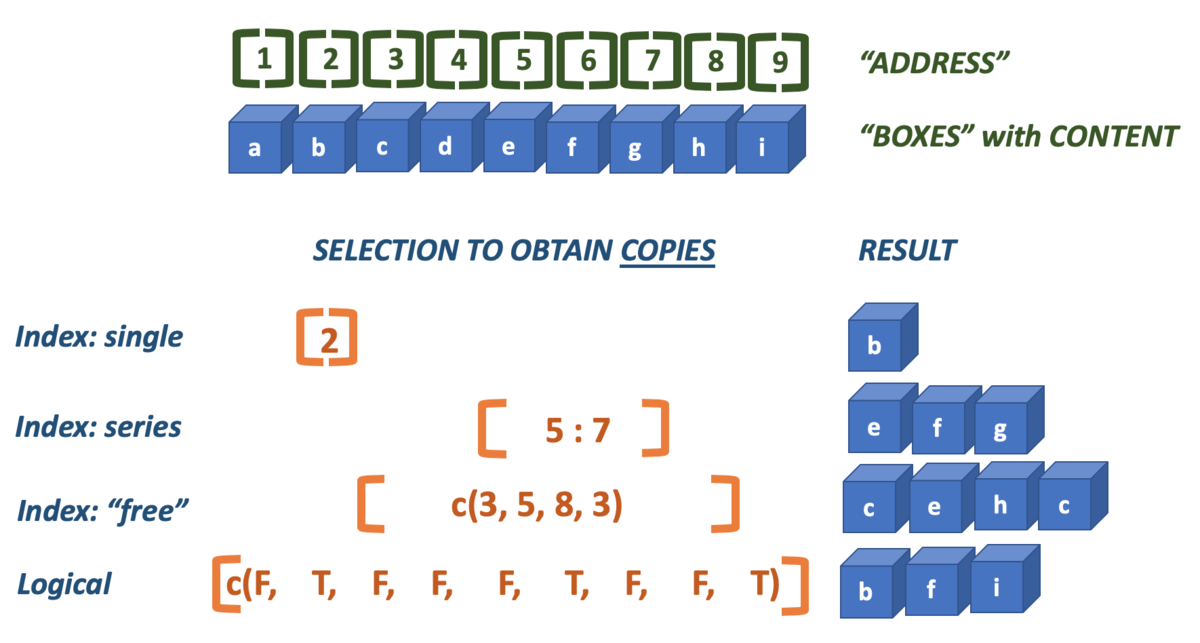
\includegraphics{figures/indexing_in_R_s.png}

The \texttt{index} is the position of a value within a vector. R starts at one (1), and therefore ends at the length of the vector. Brackets \texttt{{[}{]}} are used to specify one or more indices that should be selected (returned).

Here are two examples of straightforward indexing, selecing a single or a series of elements.

\begin{Shaded}
\begin{Highlighting}[]
\NormalTok{x <-}\StringTok{ }\KeywordTok{c}\NormalTok{(}\DecValTok{2}\NormalTok{, }\DecValTok{4}\NormalTok{, }\DecValTok{6}\NormalTok{, }\DecValTok{3}\NormalTok{, }\DecValTok{5}\NormalTok{, }\DecValTok{1}\NormalTok{)}
\NormalTok{x[}\DecValTok{4}\NormalTok{] }\CommentTok{## fourth element}
\end{Highlighting}
\end{Shaded}

\begin{verbatim}
## [1] 3
\end{verbatim}

\begin{Shaded}
\begin{Highlighting}[]
\NormalTok{x[}\DecValTok{3}\OperatorTok{:}\DecValTok{5}\NormalTok{] }\CommentTok{## elements 3 to 5}
\end{Highlighting}
\end{Shaded}

\begin{verbatim}
## [1] 6 3 5
\end{verbatim}

However, the technique is much more versatile. You can use indexing to select elements multiple times and thus create copies of them, or select elements in any order you desire.

\begin{Shaded}
\begin{Highlighting}[]
\NormalTok{x[}\KeywordTok{c}\NormalTok{(}\DecValTok{1}\NormalTok{, }\DecValTok{2}\NormalTok{, }\DecValTok{2}\NormalTok{, }\DecValTok{5}\NormalTok{)] }\CommentTok{## elements 1, 2, 2 and 5}
\end{Highlighting}
\end{Shaded}

\begin{verbatim}
## [1] 2 4 4 5
\end{verbatim}

\begin{Shaded}
\begin{Highlighting}[]
\NormalTok{x <-}\StringTok{ }\KeywordTok{c}\NormalTok{(}\DecValTok{2}\NormalTok{, }\DecValTok{4}\NormalTok{, }\DecValTok{6}\NormalTok{, }\DecValTok{3}\NormalTok{, }\DecValTok{5}\NormalTok{, }\DecValTok{1}\NormalTok{)}
\end{Highlighting}
\end{Shaded}

Besides integers you can use logicals to perform selections:

\begin{Shaded}
\begin{Highlighting}[]
\NormalTok{x[}\KeywordTok{c}\NormalTok{(T, F, T, T, T, F)]}
\end{Highlighting}
\end{Shaded}

\begin{verbatim}
## [1] 2 6 3 5
\end{verbatim}

As with all vector operations, shorter vectors are cycled as often as needed to cover the longer one:

\begin{Shaded}
\begin{Highlighting}[]
\NormalTok{x[}\KeywordTok{c}\NormalTok{(F, T, F)]}
\end{Highlighting}
\end{Shaded}

\begin{verbatim}
## [1] 4 5
\end{verbatim}

In practice you won't type literal logicals very often; they are ususaly the result of some comparison operation. Here, all even numbers are selected because their modulo will retun zero.

\begin{Shaded}
\begin{Highlighting}[]
\NormalTok{x[x }\OperatorTok\StringTok{ }\DecValTok{2} \OperatorTok{==}\StringTok{ }\DecValTok{0}\NormalTok{]}
\end{Highlighting}
\end{Shaded}

\begin{verbatim}
## [1] 2 4 6
\end{verbatim}

And all of the maximum values in a vector are retreived:

\begin{Shaded}
\begin{Highlighting}[]
\NormalTok{x <-}\StringTok{ }\KeywordTok{c}\NormalTok{(}\DecValTok{2}\NormalTok{, }\DecValTok{3}\NormalTok{, }\DecValTok{3}\NormalTok{, }\DecValTok{2}\NormalTok{, }\DecValTok{1}\NormalTok{, }\DecValTok{3}\NormalTok{)}
\NormalTok{x[x }\OperatorTok{==}\StringTok{ }\KeywordTok{max}\NormalTok{(x)]}
\end{Highlighting}
\end{Shaded}

\begin{verbatim}
## [1] 3 3 3
\end{verbatim}

There is a caveat in selecting the last \emph{n} values: the colon operator has highest precedence!
Here, the last two elements are (supposed to be selected).

\begin{Shaded}
\begin{Highlighting}[]
\NormalTok{x <-}\StringTok{ }\KeywordTok{c}\NormalTok{(}\DecValTok{2}\NormalTok{, }\DecValTok{4}\NormalTok{, }\DecValTok{6}\NormalTok{, }\DecValTok{3}\NormalTok{, }\DecValTok{5}\NormalTok{, }\DecValTok{1}\NormalTok{)}
\NormalTok{x[}\KeywordTok{length}\NormalTok{(x) }\OperatorTok{-}\StringTok{ }\DecValTok{1} \OperatorTok{:}\StringTok{ }\KeywordTok{length}\NormalTok{(x)] }\CommentTok{#fails}
\end{Highlighting}
\end{Shaded}

\begin{verbatim}
## [1] 5 3 6 4 2
\end{verbatim}

\begin{Shaded}
\begin{Highlighting}[]
\NormalTok{x[(}\KeywordTok{length}\NormalTok{(x) }\OperatorTok{-}\StringTok{ }\DecValTok{1}\NormalTok{) }\OperatorTok{:}\StringTok{ }\KeywordTok{length}\NormalTok{(x)] }\CommentTok{## parentheses required!}
\end{Highlighting}
\end{Shaded}

\begin{verbatim}
## [1] 5 1
\end{verbatim}

\hypertarget{use-which-to-get-an-index-instead-of-value}{%
\subsubsection*{\texorpdfstring{Use \texttt{which()} to get an index instead of value}{Use which() to get an index instead of value}}\label{use-which-to-get-an-index-instead-of-value}}
\addcontentsline{toc}{subsubsection}{Use \texttt{which()} to get an index instead of value}

The function \texttt{which()} returns indices for which the logical test evaluates to \texttt{true}:

\begin{Shaded}
\begin{Highlighting}[]
\KeywordTok{which}\NormalTok{(x }\OperatorTok{>=}\StringTok{ }\DecValTok{2}\NormalTok{) }\CommentTok{## which positions have values 2 or greater?}
\end{Highlighting}
\end{Shaded}

\begin{verbatim}
## [1] 1 2 3 4 5
\end{verbatim}

\begin{Shaded}
\begin{Highlighting}[]
\KeywordTok{which}\NormalTok{(x }\OperatorTok{==}\StringTok{ }\KeywordTok{max}\NormalTok{(x)) }\CommentTok{## which positions have the maximum value?}
\end{Highlighting}
\end{Shaded}

\begin{verbatim}
## [1] 3
\end{verbatim}

\hypertarget{some-coding-style-rules-rules-for-writing-code}{%
\section{Some coding style rules rules for writing code}\label{some-coding-style-rules-rules-for-writing-code}}

\begin{itemize}
\tightlist
\item
  Names of variables start with a lower-case letter
\item
  Words are separated using underscores
\item
  Be descriptive with names
\item
  Function names are verbs
\item
  Write all code and comments in English
\item
  Preferentially use one statement per line
\item
  Use spaces on both sides of ALL operators
\item
  Use a space after a comma
\item
  Indent code blocks -with \{\}- with 4 or 2 spaces, but be consistent
\end{itemize}

Follow Hadleys' style guide \url{http://adv-r.had.co.nz/Style.html}

\hypertarget{the-best-keyboard-shortcuts-for-rstudio}{%
\section{The best keyboard shortcuts for RStudio}\label{the-best-keyboard-shortcuts-for-rstudio}}

\begin{itemize}
\tightlist
\item
  \texttt{ctr\ +\ 1} go to code editor
\item
  \texttt{ctr\ +\ 2} go to console
\item
  \texttt{ctr\ +\ alt\ +\ i} insert code chunk (RMarkdown)
\item
  \texttt{ctr\ +\ enter} run current line
\item
  \texttt{ctr\ +\ shift\ +\ k} knit current document
\item
  \texttt{ctr\ +\ alt\ +\ c} run current code chunk
\item
  \texttt{ctr\ +\ shift\ +\ o} source the current document
\end{itemize}

\hypertarget{basic-r---plotting-basics}{%
\chapter{Basic R - plotting basics}\label{basic-r---plotting-basics}}

\hypertarget{basic-embedded-plot-types}{%
\section{Basic embedded plot types}\label{basic-embedded-plot-types}}

Looking at numbers is boring - people want to see pictures! Doing analyses without visualizations is like only listening to a movie.

There are a few plot types supported by base R that deal with (combinations of) vectors:

\begin{itemize}
\tightlist
\item
  scatter (or line-) plot
\item
  barplot
\item
  histogram
\item
  boxplot
\end{itemize}

We'll only look at the bare basics in this chapter because we are going to do it for real with package \texttt{ggplot2} in the next course.

\hypertarget{scatter-and-line-plots}{%
\subsection{Scatter and line plots}\label{scatter-and-line-plots}}

Meet \texttt{plot()} - the workhorse of R plotting.

\begin{Shaded}
\begin{Highlighting}[]
\NormalTok{time <-}\StringTok{ }\KeywordTok{c}\NormalTok{(}\DecValTok{1}\NormalTok{, }\DecValTok{2}\NormalTok{, }\DecValTok{3}\NormalTok{, }\DecValTok{4}\NormalTok{, }\DecValTok{5}\NormalTok{, }\DecValTok{6}\NormalTok{)}
\NormalTok{response <-}\StringTok{ }\KeywordTok{c}\NormalTok{(}\FloatTok{0.09}\NormalTok{, }\FloatTok{0.30}\NormalTok{, }\FloatTok{0.41}\NormalTok{, }\FloatTok{0.48}\NormalTok{, }\FloatTok{0.72}\NormalTok{, }\FloatTok{1.12}\NormalTok{)}
\KeywordTok{plot}\NormalTok{(}\DataTypeTok{x =}\NormalTok{ time, }\DataTypeTok{y =}\NormalTok{ response)}
\end{Highlighting}
\end{Shaded}

\begin{figure}

{\centering 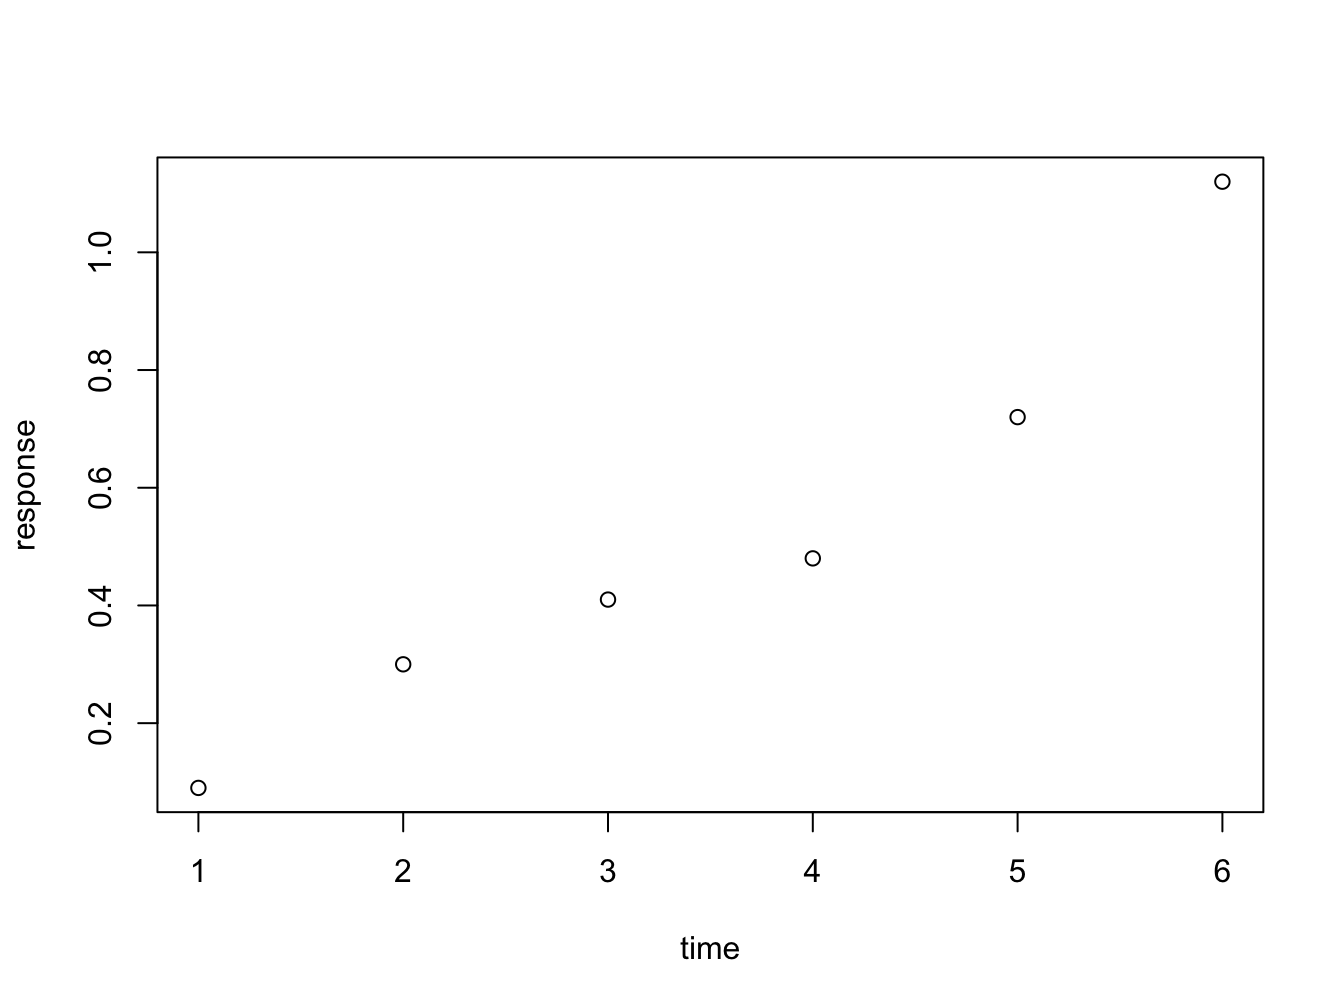
\includegraphics[width=0.8\linewidth]{davur_ebook_files/figure-latex/plot-hello-1-1} 

}

\caption{Here is a nice figure!}\label{fig:plot-hello-1}
\end{figure}

The function plot is used here to generate a \emph{scatter plot}. It may generae other types of figures, depending on its input as we'll see later.

\hypertarget{formula-notation}{%
\subsubsection*{Formula notation}\label{formula-notation}}
\addcontentsline{toc}{subsubsection}{Formula notation}

Instead of passing an \texttt{x\ =} and \texttt{y\ =} set of arguments, it is also possible to call the plot fuction with a \textbf{\emph{formula notation}}:

\begin{Shaded}
\begin{Highlighting}[]
\KeywordTok{plot}\NormalTok{(response }\OperatorTok{~}\StringTok{ }\NormalTok{time)}
\end{Highlighting}
\end{Shaded}

\begin{center}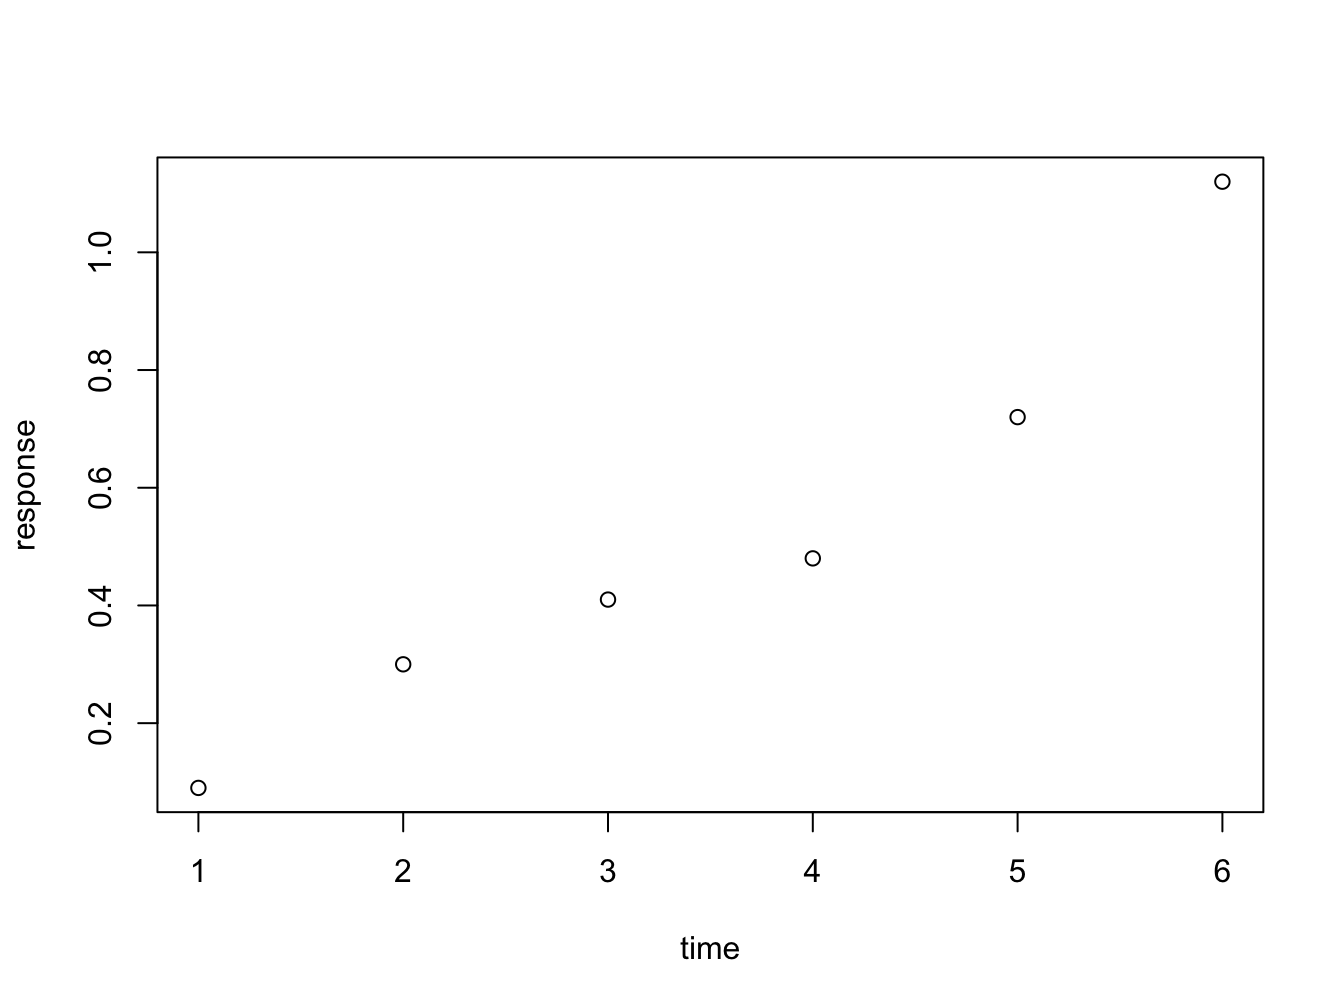
\includegraphics[width=0.8\linewidth]{davur_ebook_files/figure-latex/plot-hello-with-formula-1} \end{center}

You can read \texttt{response\ \textasciitilde{}\ time} as \emph{response as a function of time}. This is a nice, readable alternative in this case, but for many functions it is the only or preferred way to specify the relationship you want to investigate.

\hypertarget{plot-decorations}{%
\subsubsection*{Plot decorations}\label{plot-decorations}}
\addcontentsline{toc}{subsubsection}{Plot decorations}

Plots should always have these decorations:

\begin{itemize}
\tightlist
\item
  Axis labels indicating measurement type (quantity) and its units. E.g. `{[}Mg{]} (mq/ml)' or `Heartrate (bpm)'.
\item
  If multiple data series are plotted: a legend
\item
  Either a title or a figure caption, depending on the context.
\end{itemize}

The first plots of this chapters were very bare (and a bit boring to look at): the plot has no axis labels (quantity and units) and no decoration whatsoever. By passing arguments to \texttt{plot()} you can modify or add many features of your plot. Basic decoration includes

\begin{itemize}
\tightlist
\item
  adjusting markers (\texttt{pch\ =\ 19}, \texttt{col\ =\ "blue"})
\item
  adding connector lines (\texttt{type\ =\ "b"}) or removing points (\texttt{type\ =\ "l"})
\item
  adding axis labels and title (\texttt{xlab\ =\ "Time\ (hours)"}, \texttt{ylab\ =\ "Systemic\ response"}, \texttt{main\ =\ "Systemic\ response\ to\ agent\ X"})
\item
  adjusting axis limits (\texttt{xlim\ =\ c(0,\ 8)})
\end{itemize}

This is not an exhaustive listing; these are listed in the last section of this chapter.

Here is a more complete plot using a variety of arguments.

\begin{Shaded}
\begin{Highlighting}[]
\KeywordTok{plot}\NormalTok{(}\DataTypeTok{x =}\NormalTok{ time, }\DataTypeTok{y =}\NormalTok{ response, }\DataTypeTok{pch =} \DecValTok{19}\NormalTok{, }\DataTypeTok{type =} \StringTok{"b"}\NormalTok{, }\DataTypeTok{xlim =} \KeywordTok{c}\NormalTok{(}\DecValTok{0}\NormalTok{, }\DecValTok{8}\NormalTok{),}
     \DataTypeTok{xlab =} \StringTok{"Time (hours)"}\NormalTok{, }\DataTypeTok{ylab =} \StringTok{"Systemic response (a.u.)"}\NormalTok{,}
     \DataTypeTok{main =} \StringTok{"Systemic response to agent X"}\NormalTok{, }\DataTypeTok{col =} \StringTok{"blue"}\NormalTok{)}
\end{Highlighting}
\end{Shaded}

\begin{center}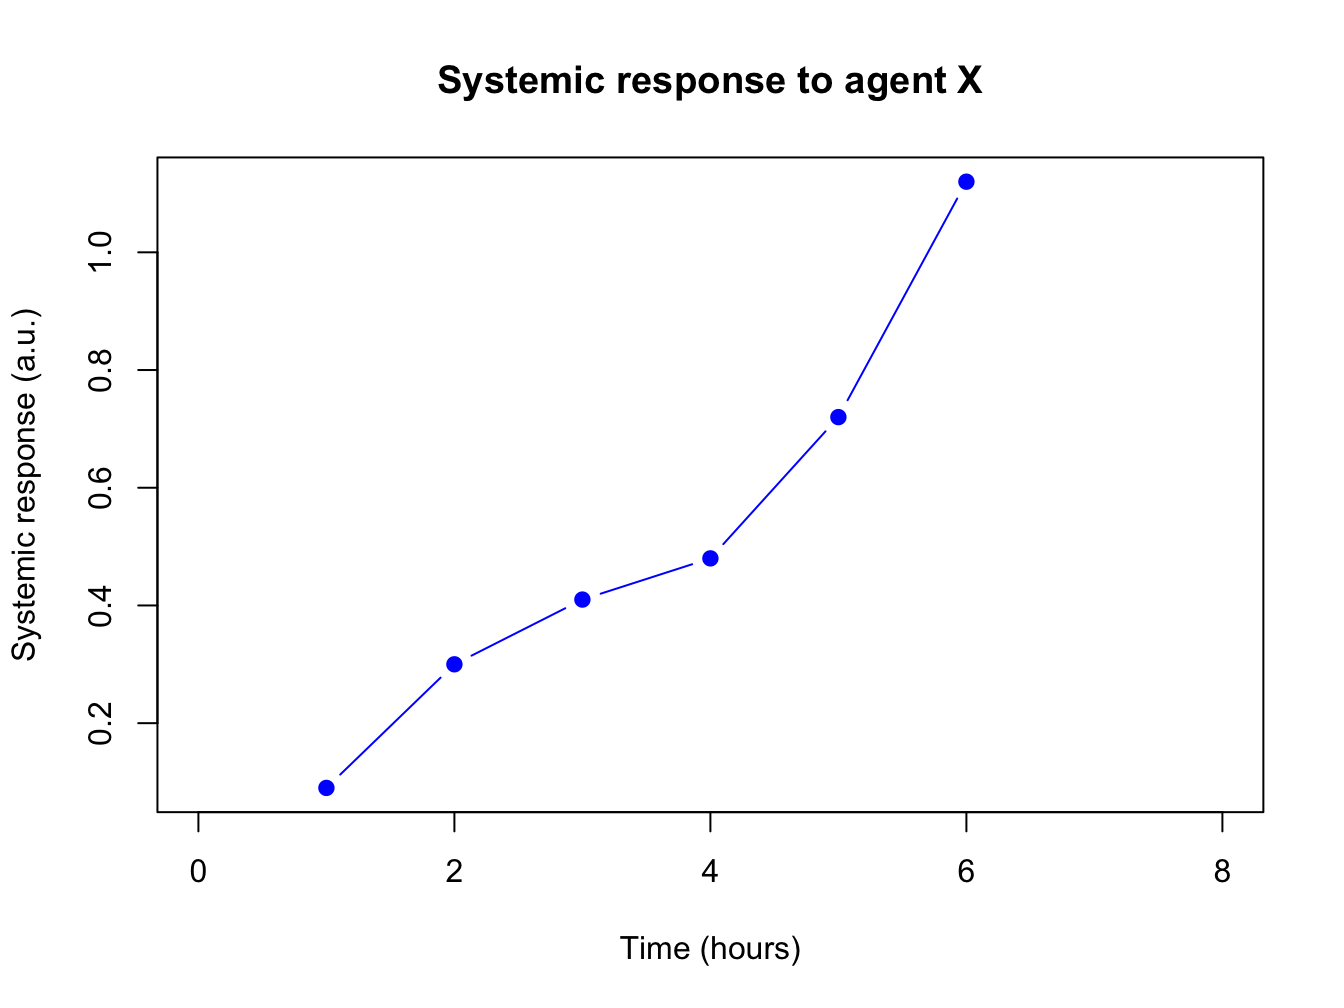
\includegraphics[width=0.8\linewidth]{davur_ebook_files/figure-latex/plot-hello-2-1} \end{center}

\hypertarget{adjusting-the-plot-symbol}{%
\subsubsection*{Adjusting the plot symbol}\label{adjusting-the-plot-symbol}}
\addcontentsline{toc}{subsubsection}{Adjusting the plot symbol}

When you have many data points they will overlap. Using transparency with the \texttt{rgb(,,\ alpha=)} color definition and/or smaller plot symbols (\texttt{cex=}) solves this.

\begin{Shaded}
\begin{Highlighting}[]
\NormalTok{x <-}\StringTok{ }\KeywordTok{rnorm}\NormalTok{(}\DecValTok{1000}\NormalTok{, }\DecValTok{10}\NormalTok{, }\DecValTok{2}\NormalTok{); y <-}\StringTok{ }\NormalTok{x }\OperatorTok{+}\StringTok{ }\KeywordTok{rnorm}\NormalTok{(}\DecValTok{1000}\NormalTok{, }\FloatTok{0.5}\NormalTok{, }\FloatTok{0.5}\NormalTok{)}
\KeywordTok{plot}\NormalTok{(x, y, }\DataTypeTok{pch =} \DecValTok{19}\NormalTok{, }\DataTypeTok{cex =} \FloatTok{0.6}\NormalTok{,}
     \DataTypeTok{col =} \KeywordTok{rgb}\NormalTok{(}\DataTypeTok{red =} \DecValTok{0}\NormalTok{, }\DataTypeTok{green =} \DecValTok{0}\NormalTok{, }\DataTypeTok{blue =} \DecValTok{1}\NormalTok{, }\DataTypeTok{alpha =} \FloatTok{0.2}\NormalTok{))}
\end{Highlighting}
\end{Shaded}

\begin{center}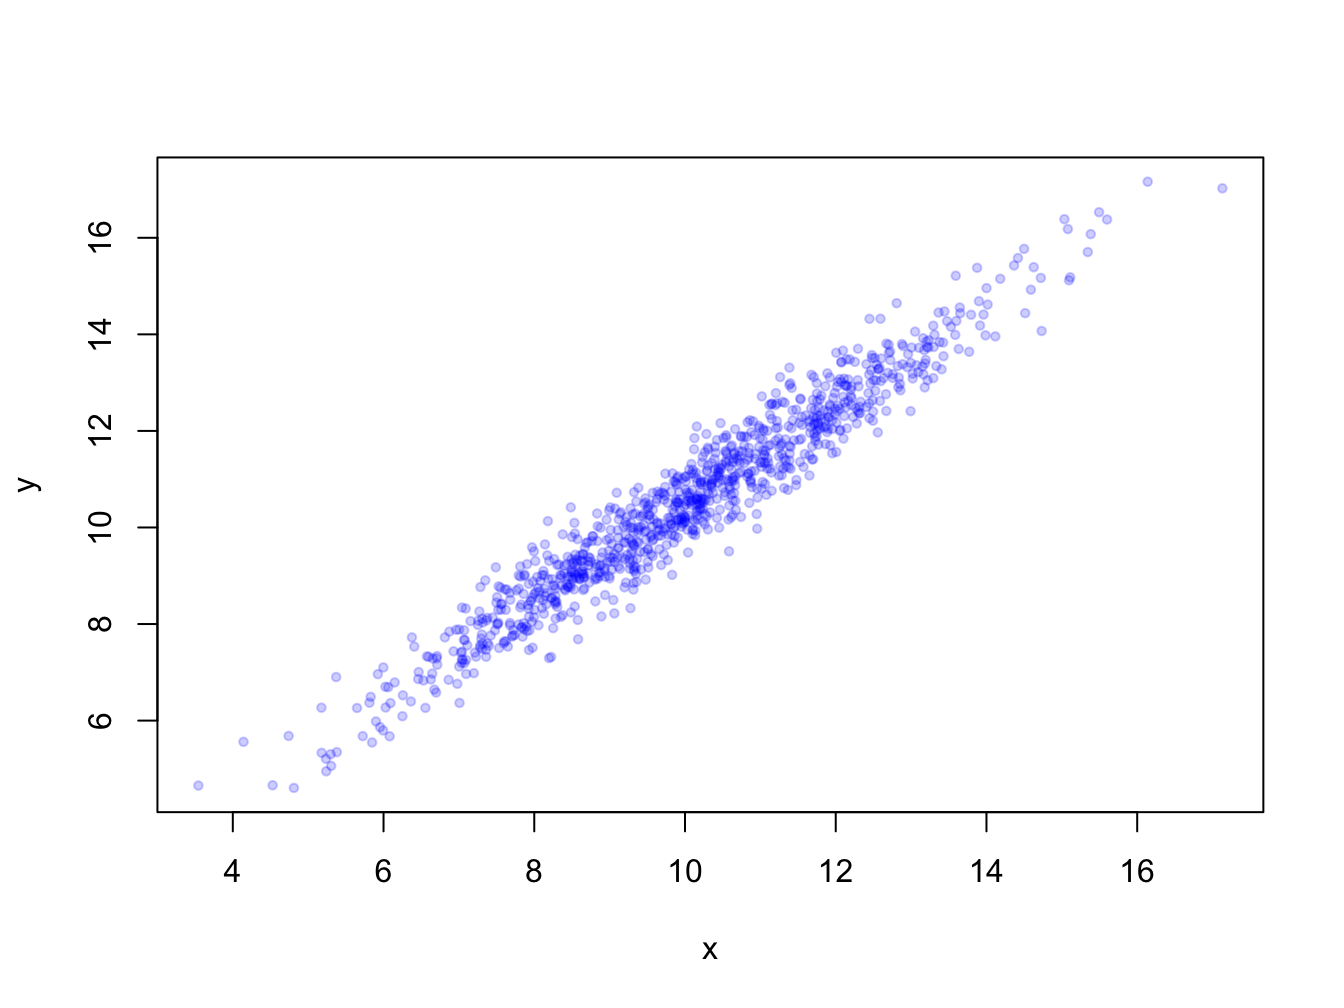
\includegraphics[width=0.8\linewidth]{davur_ebook_files/figure-latex/plot-hello-3-1} \end{center}

\hypertarget{barplots}{%
\subsection{Barplots}\label{barplots}}

Barplots can be generated in several ways:

\begin{itemize}
\tightlist
\item
  By passing a factor to \texttt{plot()} - it will generate a barplot of level frequencies. This is a shorthand for \texttt{barplot(table(some\_factor))}.
\item
  By using \texttt{barplot()}. The advantage of this is that accepts some graphical parameters that are not relevant and accepted by \texttt{plot()}, such as \texttt{beside\ =}, \texttt{height\ =}, \texttt{width\ =} and others (type \texttt{?barplot} to see all).
\end{itemize}

Here is an example:

\begin{Shaded}
\begin{Highlighting}[]
\NormalTok{persons <-}\StringTok{ }\KeywordTok{as.factor}\NormalTok{(}\KeywordTok{sample}\NormalTok{(}\KeywordTok{c}\NormalTok{(}\StringTok{"male"}\NormalTok{, }\StringTok{"female"}\NormalTok{), }\DataTypeTok{size =} \DecValTok{100}\NormalTok{, }\DataTypeTok{replace =}\NormalTok{ T))}
\KeywordTok{plot}\NormalTok{(persons)}
\end{Highlighting}
\end{Shaded}

\begin{center}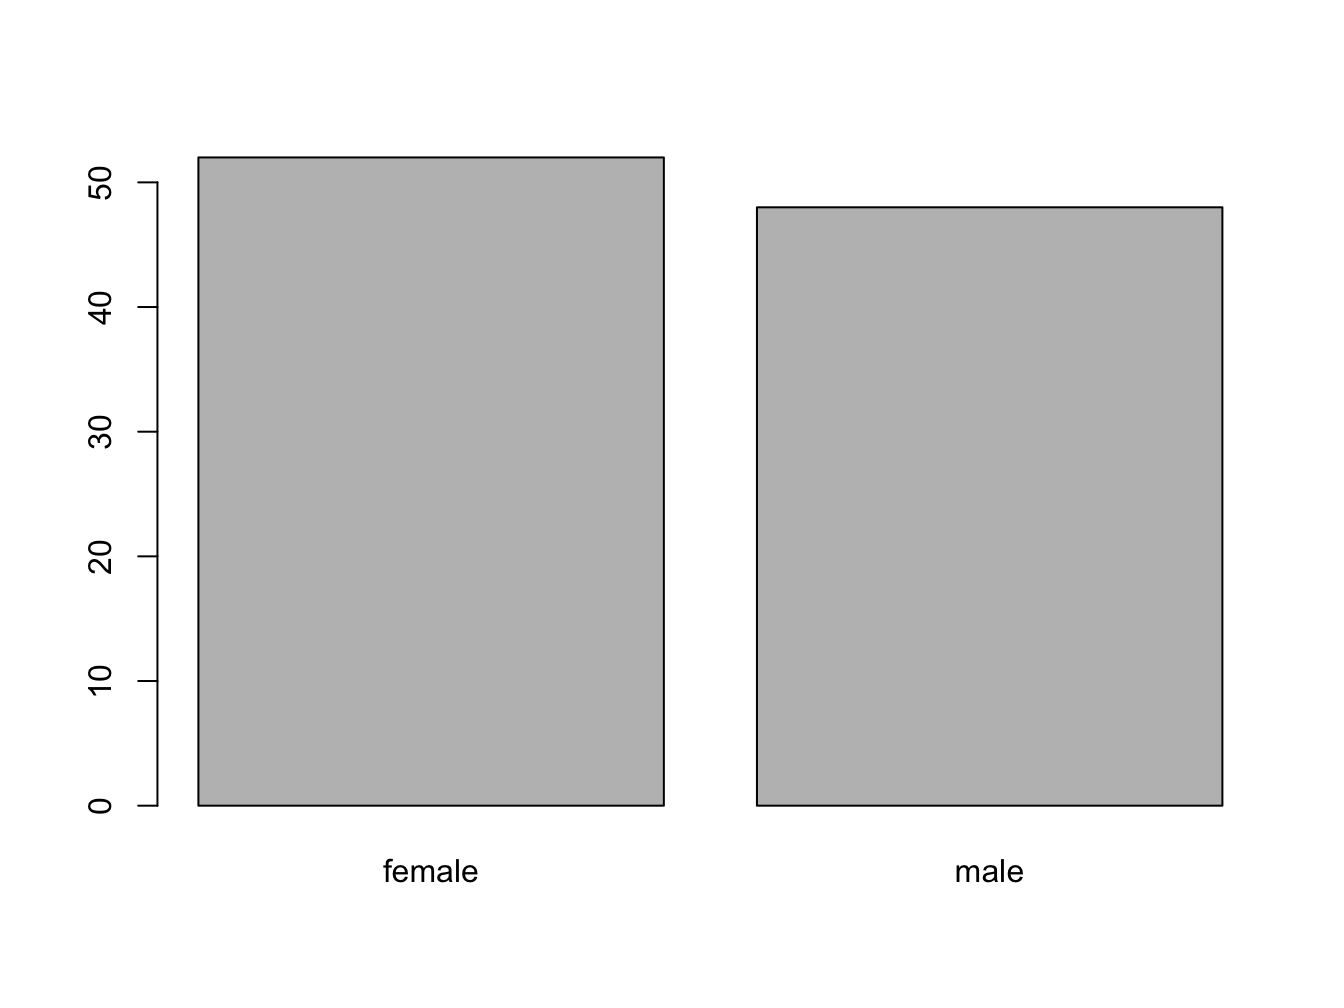
\includegraphics[width=0.8\linewidth]{davur_ebook_files/figure-latex/barplot-0-1} \end{center}

\hypertarget{barplot-with-a-vector}{%
\subsubsection*{\texorpdfstring{\texttt{barplot()} with a vector}{barplot() with a vector}}\label{barplot-with-a-vector}}
\addcontentsline{toc}{subsubsection}{\texttt{barplot()} with a vector}

The function \texttt{barplot()} can be called with a vector specifying the bar heights (frequencies), or a \texttt{table} object.

\begin{Shaded}
\begin{Highlighting}[]
\NormalTok{frequencies <-}\StringTok{ }\KeywordTok{c}\NormalTok{(}\DecValTok{22}\NormalTok{, }\DecValTok{54}\NormalTok{, }\DecValTok{12}\NormalTok{, }\DecValTok{29}\NormalTok{)}
\KeywordTok{barplot}\NormalTok{(frequencies, }\DataTypeTok{names =} \KeywordTok{c}\NormalTok{(}\StringTok{"one"}\NormalTok{, }\StringTok{"two"}\NormalTok{, }\StringTok{"three"}\NormalTok{, }\StringTok{"four"}\NormalTok{))}
\end{Highlighting}
\end{Shaded}

\begin{center}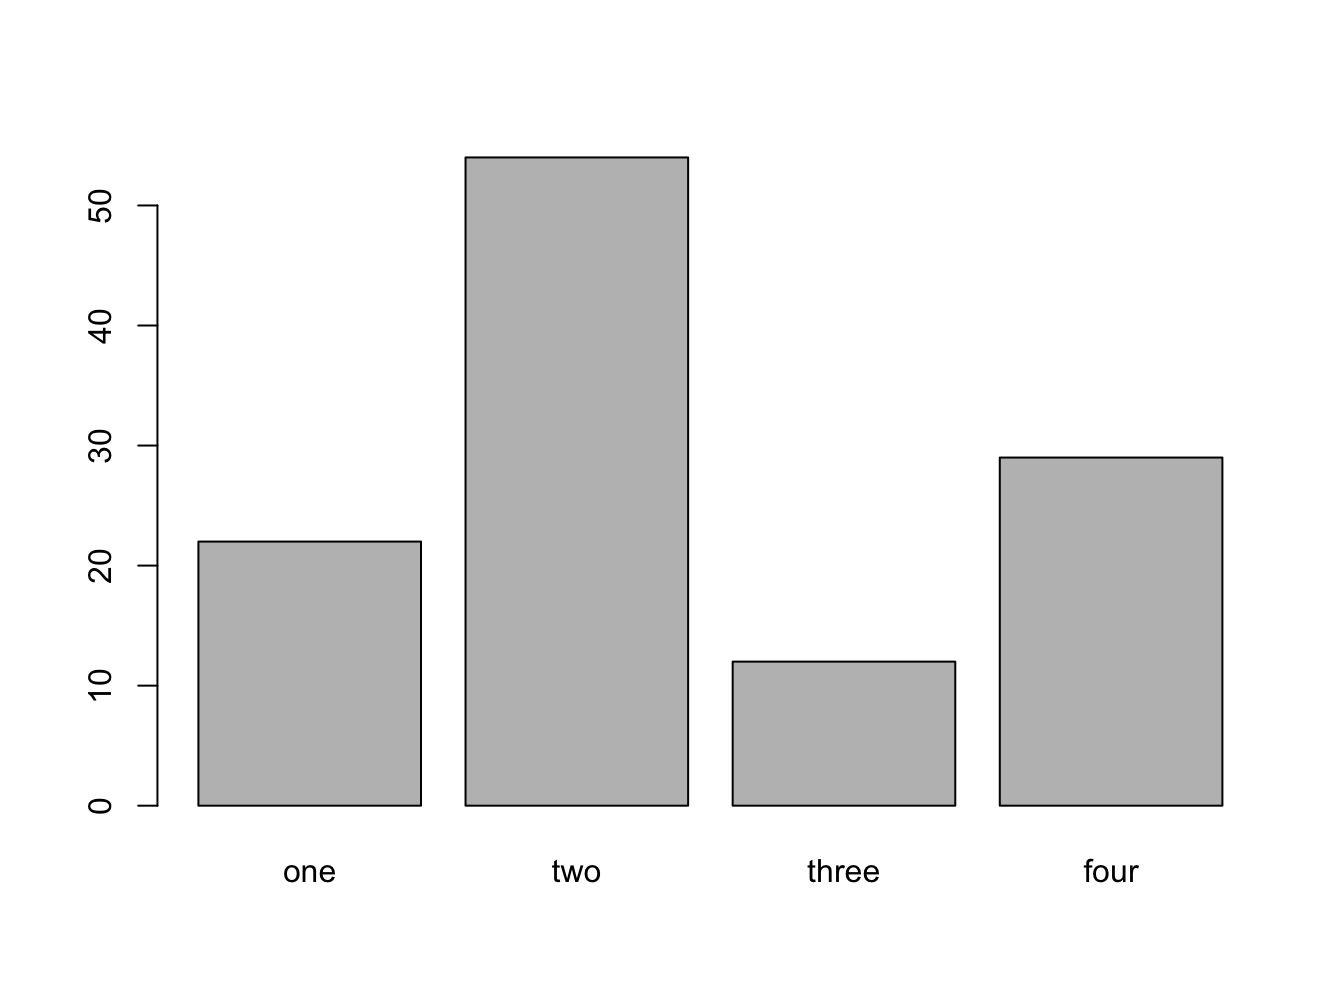
\includegraphics[width=0.8\linewidth]{davur_ebook_files/figure-latex/barplot-1-1} \end{center}

With a table object:

\begin{Shaded}
\begin{Highlighting}[]
\KeywordTok{table}\NormalTok{(persons)}
\end{Highlighting}
\end{Shaded}

\begin{verbatim}
## persons
## female   male 
##     46     54
\end{verbatim}

\begin{Shaded}
\begin{Highlighting}[]
\KeywordTok{barplot}\NormalTok{(}\KeywordTok{table}\NormalTok{(persons))}
\end{Highlighting}
\end{Shaded}

\begin{center}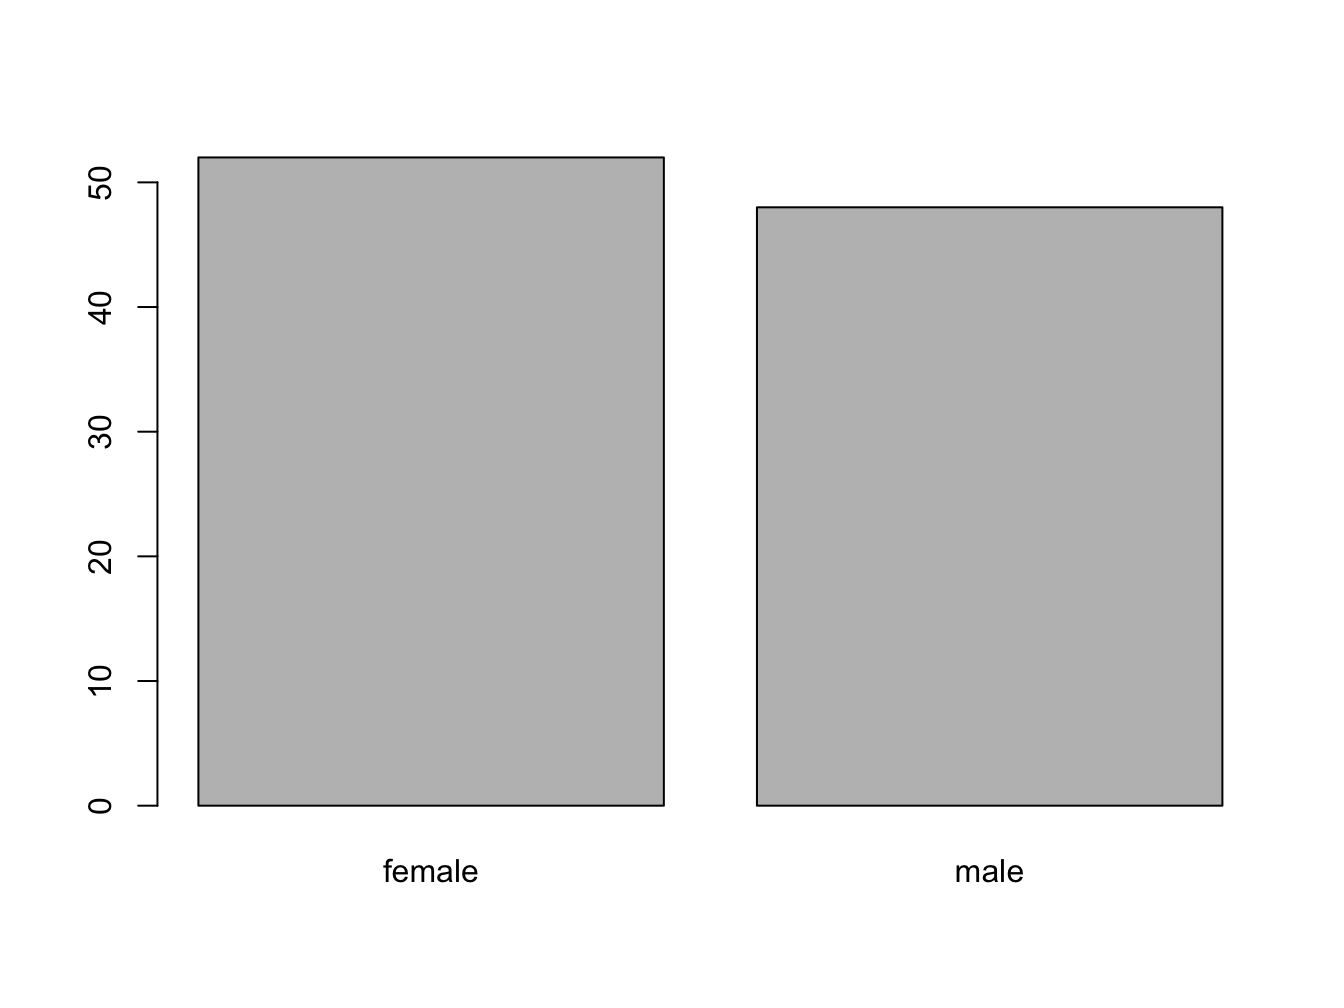
\includegraphics[width=0.8\linewidth]{davur_ebook_files/figure-latex/barplot-2-1} \end{center}

\hypertarget{barplot-with-a-2d-table-object}{%
\subsubsection*{\texorpdfstring{\texttt{barplot()} with a 2D table object}{barplot() with a 2D table object}}\label{barplot-with-a-2d-table-object}}
\addcontentsline{toc}{subsubsection}{\texttt{barplot()} with a 2D table object}

Suppose you have this data:

\begin{Shaded}
\begin{Highlighting}[]
\KeywordTok{set.seed}\NormalTok{(}\DecValTok{1234}\NormalTok{) }
\NormalTok{course <-}\StringTok{ }\KeywordTok{rep}\NormalTok{(}\KeywordTok{c}\NormalTok{(}\StringTok{"biology"}\NormalTok{, }\StringTok{"chemistry"}\NormalTok{), }\DataTypeTok{each =} \DecValTok{10}\NormalTok{)}
\NormalTok{passed <-}\StringTok{ }\KeywordTok{sample}\NormalTok{(}\KeywordTok{c}\NormalTok{(}\StringTok{"Passed"}\NormalTok{, }\StringTok{"Failed"}\NormalTok{), }\DataTypeTok{size =} \DecValTok{20}\NormalTok{, }\DataTypeTok{replace =}\NormalTok{ T)}
\NormalTok{tbl <-}\StringTok{ }\KeywordTok{table}\NormalTok{(passed, course) }\CommentTok{# the order matters!}
\NormalTok{tbl}
\end{Highlighting}
\end{Shaded}

\begin{verbatim}
##         course
## passed   biology chemistry
##   Failed       6         8
##   Passed       4         2
\end{verbatim}

The \texttt{set.seed(1234)} makes the \emph{sampling} reproducible, although that sounds really unlogical. Discussing \textbf{\emph{pseudorandom}} sampling is not within the scope of this course however.

You can create a \textbf{\emph{stacked bar chart}} like this.

\begin{Shaded}
\begin{Highlighting}[]
\KeywordTok{barplot}\NormalTok{(tbl, }
        \DataTypeTok{col =} \KeywordTok{c}\NormalTok{(}\StringTok{"red"}\NormalTok{, }\StringTok{"darkblue"}\NormalTok{), }
        \DataTypeTok{xlim =} \KeywordTok{c}\NormalTok{(}\DecValTok{0}\NormalTok{, }\KeywordTok{ncol}\NormalTok{(tbl) }\OperatorTok{+}\StringTok{ }\DecValTok{2}\NormalTok{), }
        \DataTypeTok{legend =} \KeywordTok{rownames}\NormalTok{(tbl))}
\end{Highlighting}
\end{Shaded}

\begin{center}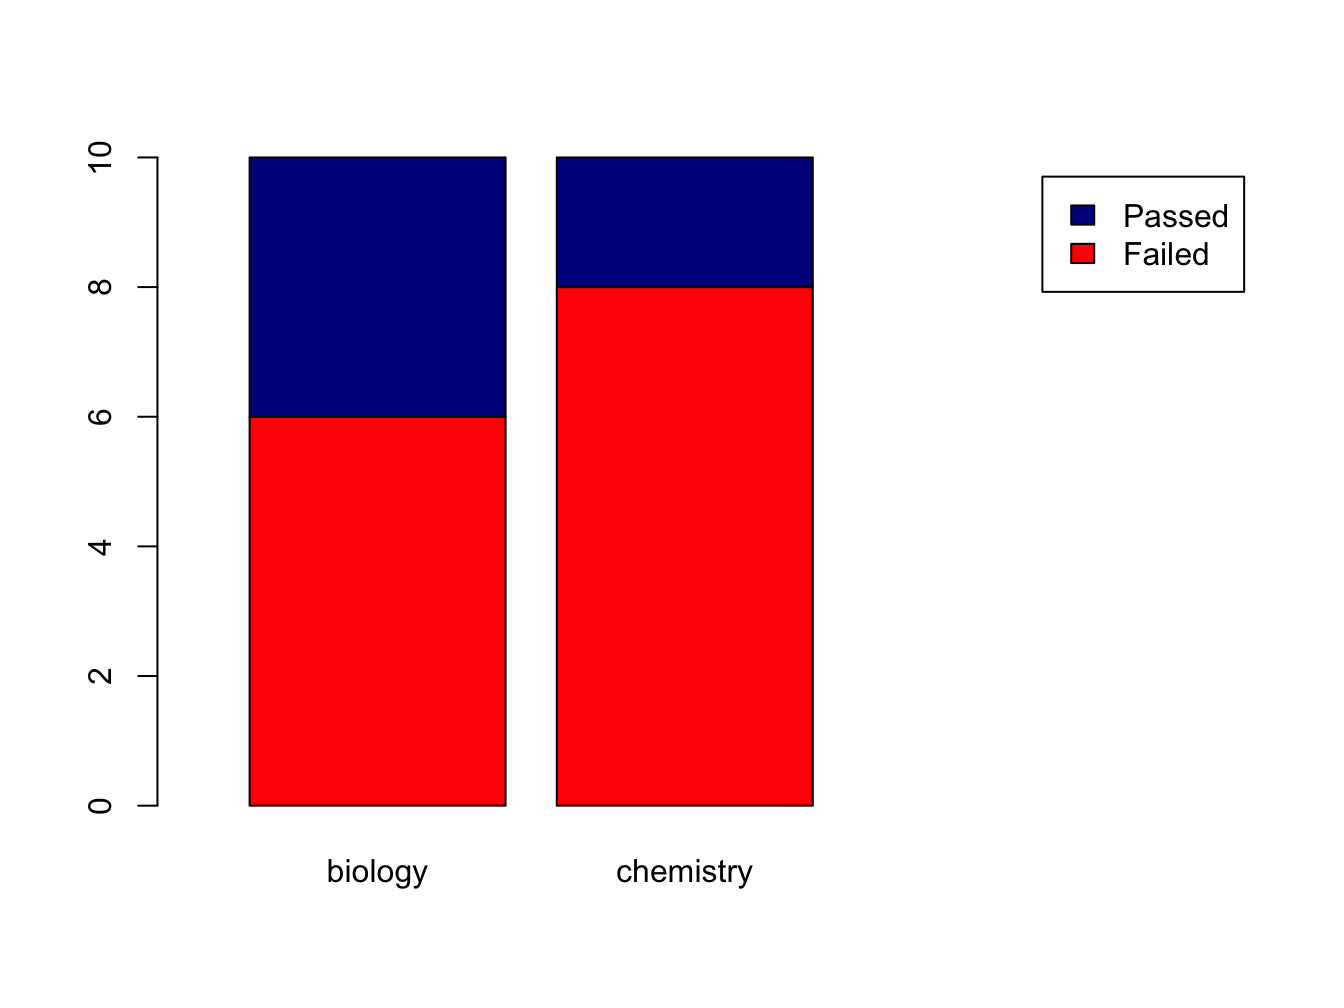
\includegraphics[width=0.8\linewidth]{davur_ebook_files/figure-latex/barplot-4-1} \end{center}

The \texttt{xlim\ =} setting is a trick to get the legend beside the plot.

Using the \texttt{beside\ =\ TRUE} argument, you get the bars \textbf{\emph{side by side}}:

\begin{Shaded}
\begin{Highlighting}[]
\KeywordTok{barplot}\NormalTok{(tbl, }
        \DataTypeTok{col=}\KeywordTok{c}\NormalTok{(}\StringTok{"red"}\NormalTok{, }\StringTok{"darkblue"}\NormalTok{), }
        \DataTypeTok{beside =} \OtherTok{TRUE}\NormalTok{, }
        \DataTypeTok{xlim=}\KeywordTok{c}\NormalTok{(}\DecValTok{0}\NormalTok{, }\KeywordTok{ncol}\NormalTok{(tbl)}\OperatorTok{*}\DecValTok{2} \OperatorTok{+}\StringTok{ }\DecValTok{3}\NormalTok{), }
        \DataTypeTok{legend =} \KeywordTok{rownames}\NormalTok{(tbl))}
\end{Highlighting}
\end{Shaded}

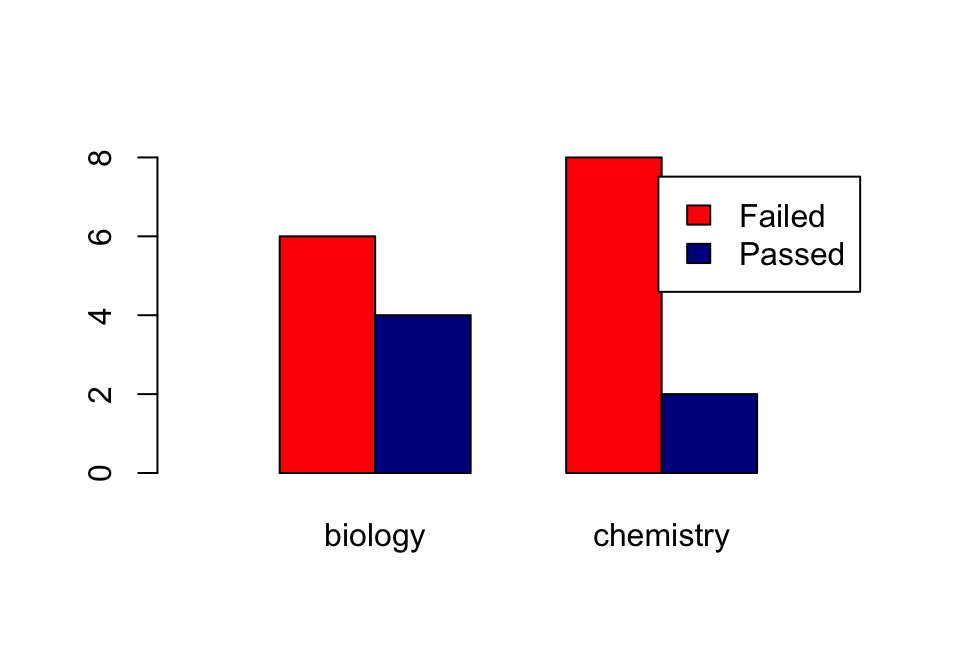
\includegraphics{davur_ebook_files/figure-latex/barplot-5-1.pdf}

Later, we'll see another data structure to feed to barplot: the matrix.

\hypertarget{histograms}{%
\subsection{Histograms}\label{histograms}}

Histograms help you visualise the distribution of your data.

\begin{Shaded}
\begin{Highlighting}[]
\NormalTok{male_weights <-}\StringTok{ }\KeywordTok{c}\NormalTok{(}\KeywordTok{rnorm}\NormalTok{(}\DecValTok{500}\NormalTok{, }\DecValTok{80}\NormalTok{, }\DecValTok{8}\NormalTok{)) }\CommentTok{## create 500 random numbers around 80}
\KeywordTok{hist}\NormalTok{(male_weights)}
\end{Highlighting}
\end{Shaded}

\begin{center}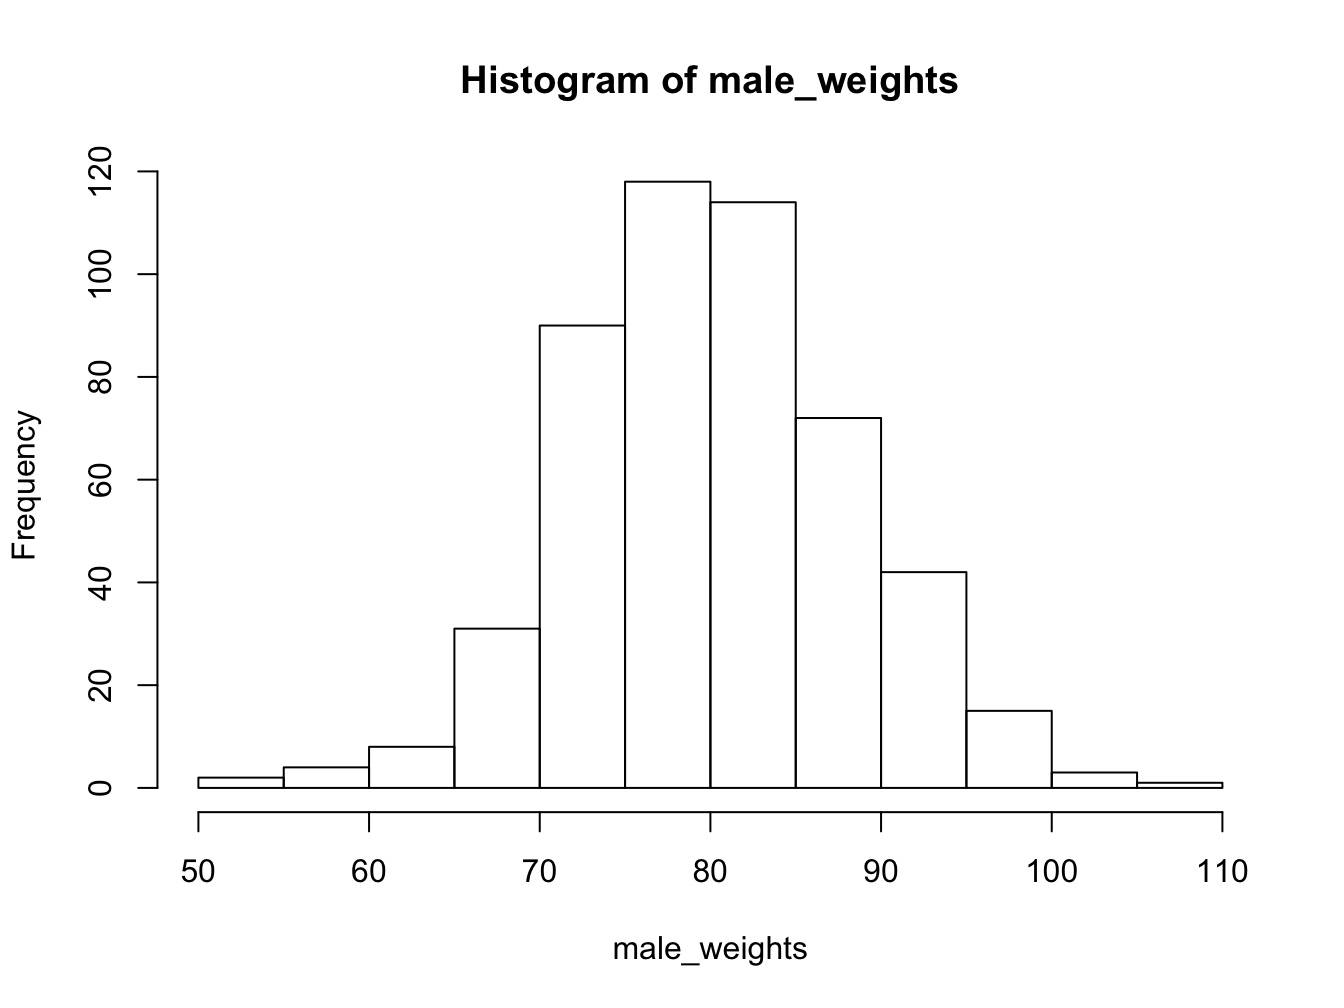
\includegraphics[width=0.8\linewidth]{davur_ebook_files/figure-latex/histogram-1-1} \end{center}

Using the \texttt{breaks} argument, you can adjust the bin width. Always explore this option when creating histograms!

\begin{Shaded}
\begin{Highlighting}[]
\KeywordTok{par}\NormalTok{(}\DataTypeTok{mfrow =} \KeywordTok{c}\NormalTok{(}\DecValTok{1}\NormalTok{, }\DecValTok{2}\NormalTok{)) }\CommentTok{# make 2 plots to sit side by side}
\KeywordTok{hist}\NormalTok{(male_weights, }\DataTypeTok{breaks =} \DecValTok{5}\NormalTok{, }\DataTypeTok{col =} \StringTok{"gold"}\NormalTok{, }\DataTypeTok{main =} \StringTok{"Male weights"}\NormalTok{)}
\KeywordTok{hist}\NormalTok{(male_weights, }\DataTypeTok{breaks =} \DecValTok{25}\NormalTok{, }\DataTypeTok{col =} \StringTok{"green"}\NormalTok{, }\DataTypeTok{main =} \StringTok{"Male weights"}\NormalTok{)}
\end{Highlighting}
\end{Shaded}

\begin{center}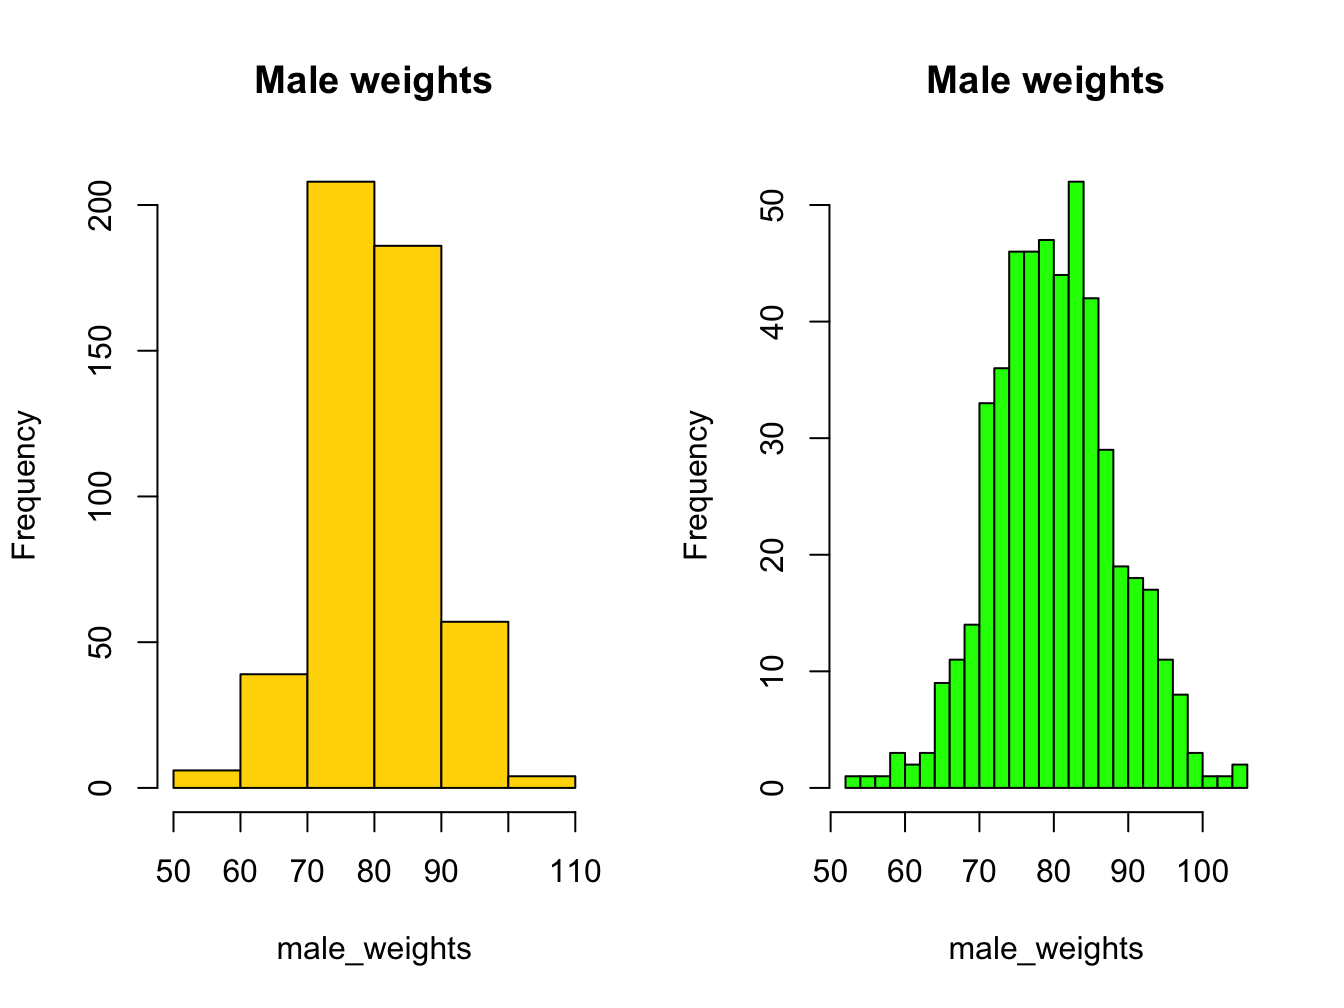
\includegraphics[width=0.8\linewidth]{davur_ebook_files/figure-latex/histogram-2-1} \end{center}

If you want a more detailed

\hypertarget{density-plot-as-alternative-to-hist}{%
\subsection{\texorpdfstring{Density plot as alternative to \texttt{hist()}}{Density plot as alternative to hist()}}\label{density-plot-as-alternative-to-hist}}

When you want a bit more fine-grained view of the distribution you can use a plot of a density function; by adding a \texttt{polygon()} you can even have some nice shading under the line:

\begin{Shaded}
\begin{Highlighting}[]
\KeywordTok{plot}\NormalTok{(}\KeywordTok{density}\NormalTok{(male_weights),}
     \DataTypeTok{main =} \StringTok{"A density plot of male weights"}\NormalTok{,}
     \DataTypeTok{col =} \StringTok{"blue"}\NormalTok{, }\DataTypeTok{lwd =} \DecValTok{2}\NormalTok{)}
\KeywordTok{polygon}\NormalTok{(}\KeywordTok{density}\NormalTok{(male_weights), }\DataTypeTok{col=}\StringTok{"lightblue"}\NormalTok{)}
\end{Highlighting}
\end{Shaded}

\begin{center}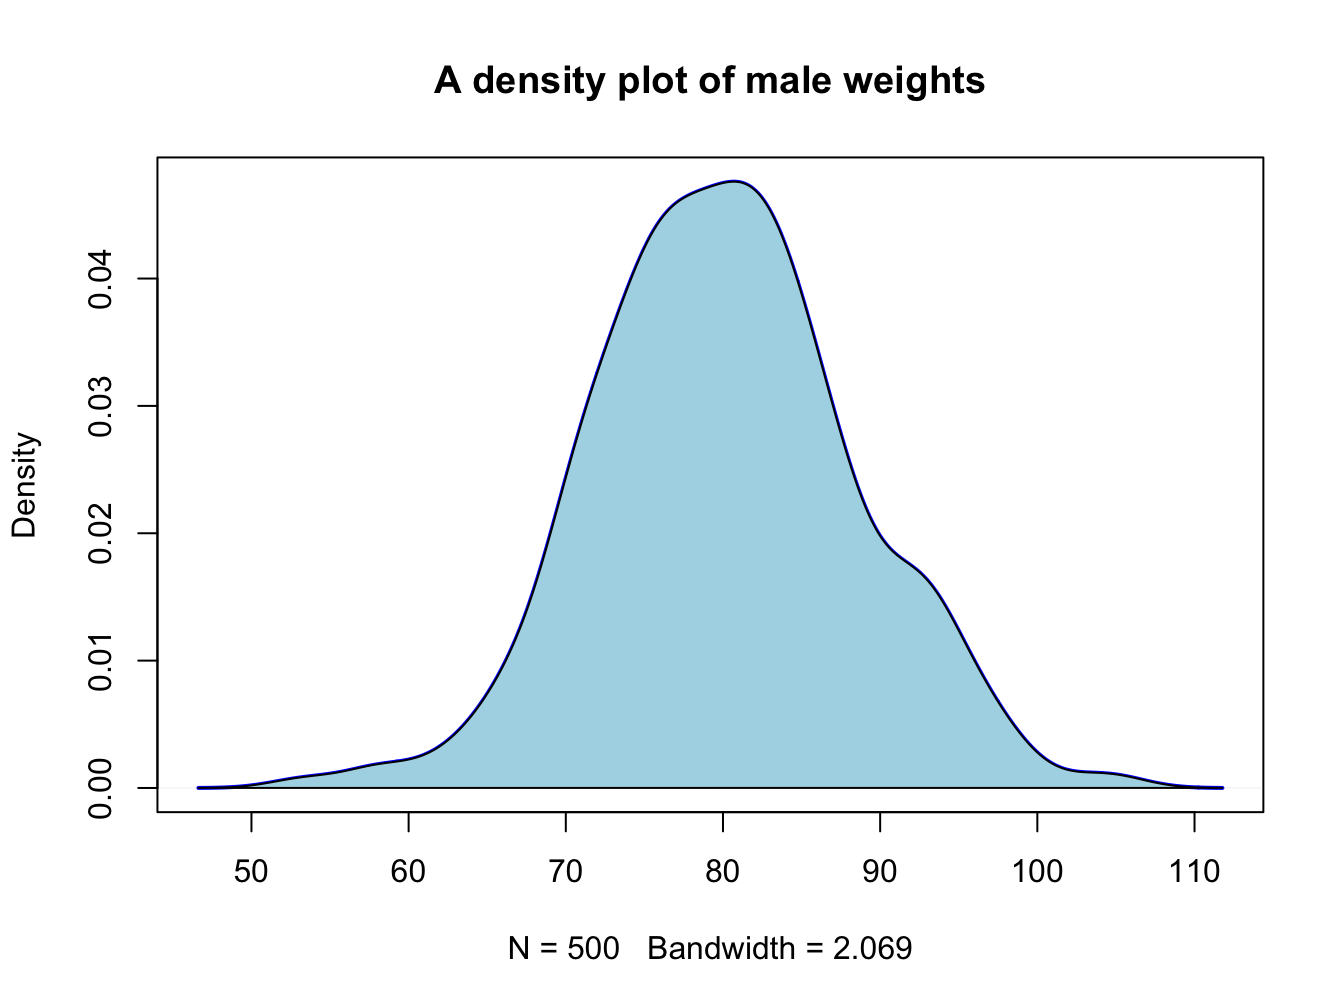
\includegraphics[width=0.8\linewidth]{davur_ebook_files/figure-latex/density-plot-1-1} \end{center}

\hypertarget{boxplots}{%
\subsection{Boxplots}\label{boxplots}}

This is the last of the basic plot types. A boxplot is a visual representation of the \emph{5-number summary} of a numeric variable: minimum, maximum, median, first and third quartile.

\begin{Shaded}
\begin{Highlighting}[]
\NormalTok{persons <-}\StringTok{ }\KeywordTok{rep}\NormalTok{(}\KeywordTok{c}\NormalTok{(}\StringTok{"male"}\NormalTok{, }\StringTok{"female"}\NormalTok{), }\DataTypeTok{each =} \DecValTok{100}\NormalTok{)}
\NormalTok{weights <-}\StringTok{ }\KeywordTok{c}\NormalTok{(}\KeywordTok{rnorm}\NormalTok{(}\DecValTok{100}\NormalTok{, }\DecValTok{80}\NormalTok{, }\DecValTok{6}\NormalTok{), }\KeywordTok{rnorm}\NormalTok{(}\DecValTok{100}\NormalTok{, }\DecValTok{75}\NormalTok{, }\DecValTok{8}\NormalTok{))}
\CommentTok{#print 6-number summary (5-number + mean)}
\KeywordTok{summary}\NormalTok{(weights[persons }\OperatorTok{==}\StringTok{ "female"}\NormalTok{])}
\end{Highlighting}
\end{Shaded}

\begin{verbatim}
##    Min. 1st Qu.  Median    Mean 3rd Qu.    Max. 
##    57.7    69.4    74.1    74.0    79.0    92.2
\end{verbatim}

Boxplots tell the same story as histograms, but are less precise. however, they are excellent when you want to show a series of subsets split over some variable.

\begin{Shaded}
\begin{Highlighting}[]
\KeywordTok{par}\NormalTok{(}\DataTypeTok{mfrow =} \KeywordTok{c}\NormalTok{(}\DecValTok{1}\NormalTok{, }\DecValTok{2}\NormalTok{)) }\CommentTok{# make 2 plots to sit side by side}
\CommentTok{# create boxplots of weights depending on sex}
\KeywordTok{boxplot}\NormalTok{(weights }\OperatorTok{~}\StringTok{ }\NormalTok{persons, }\DataTypeTok{ylab =} \StringTok{"weight"}\NormalTok{)}
\KeywordTok{boxplot}\NormalTok{(weights }\OperatorTok{~}\StringTok{ }\NormalTok{persons, }\DataTypeTok{notch =} \OtherTok{TRUE}\NormalTok{, }\DataTypeTok{col =} \KeywordTok{c}\NormalTok{(}\StringTok{"yellow"}\NormalTok{, }\StringTok{"magenta"}\NormalTok{))}
\end{Highlighting}
\end{Shaded}

\begin{center}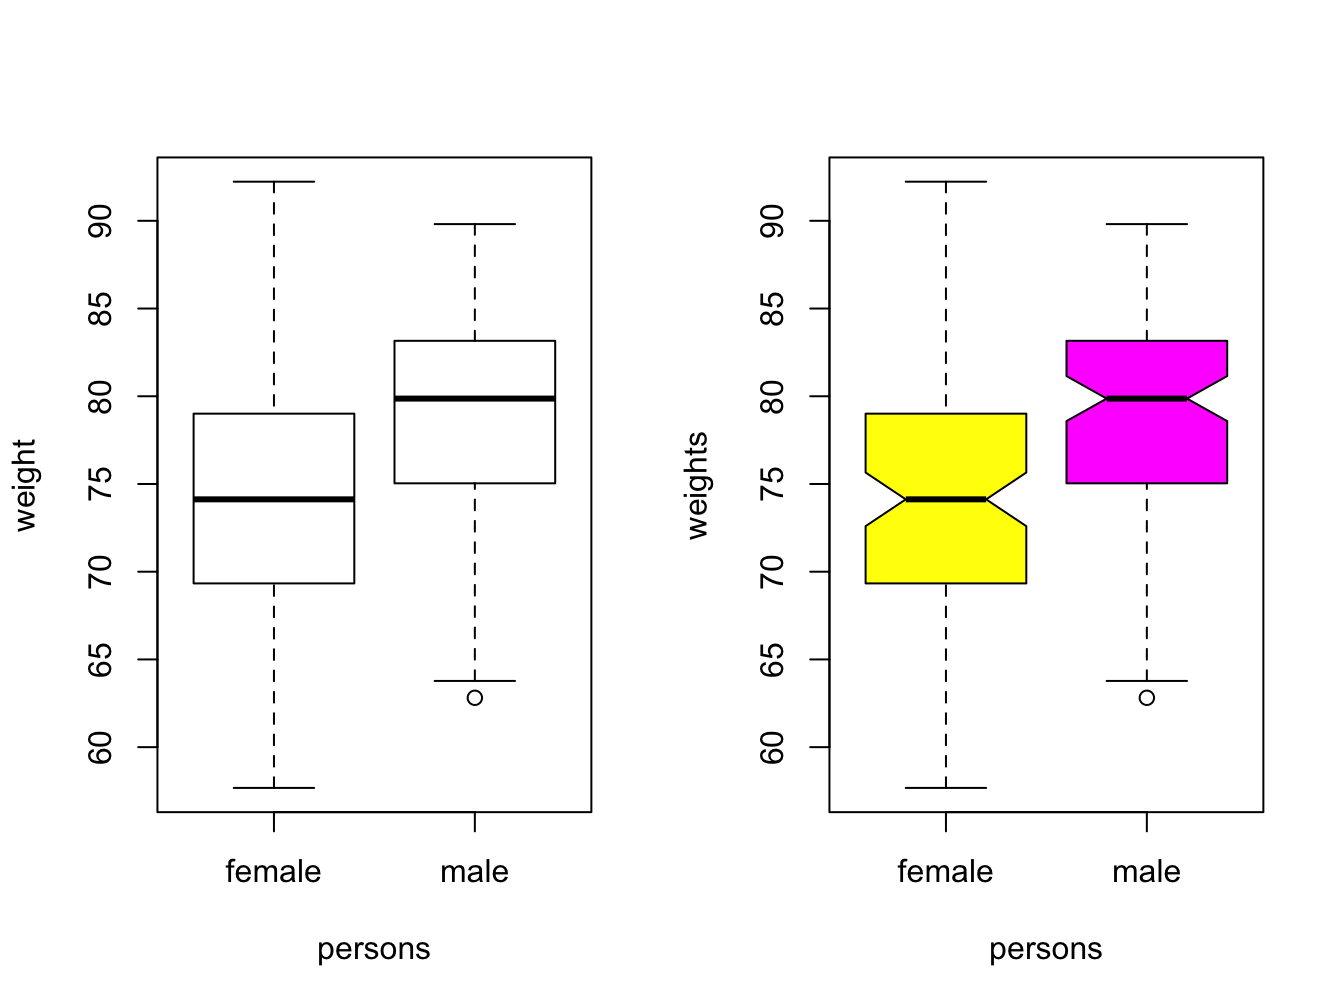
\includegraphics[width=0.8\linewidth]{davur_ebook_files/figure-latex/boxplots-1-1} \end{center}

Use \texttt{varwidth\ =\ TRUE} when you want to visualize the difference in group sizes.

\hypertarget{adding-more-data-and-a-legend}{%
\subsection{Adding more data and a legend}\label{adding-more-data-and-a-legend}}

When you have more than one data series to plot, add them using the function \texttt{points()}. You call this function \emph{after} you created the primary plot. Since there are multiple lines you will also need a legend.

\begin{Shaded}
\begin{Highlighting}[]
\NormalTok{response2 <-}\StringTok{ }\KeywordTok{c}\NormalTok{(}\FloatTok{0.07}\NormalTok{, }\FloatTok{0.10}\NormalTok{, }\FloatTok{0.17}\NormalTok{, }\FloatTok{0.28}\NormalTok{, }\FloatTok{0.46}\NormalTok{, }\FloatTok{0.61}\NormalTok{)}
\KeywordTok{plot}\NormalTok{(}\DataTypeTok{x =}\NormalTok{ time, }\DataTypeTok{y =}\NormalTok{ response, }\DataTypeTok{pch =} \DecValTok{19}\NormalTok{, }\DataTypeTok{type =} \StringTok{"b"}\NormalTok{,}
     \DataTypeTok{xlab =} \StringTok{"Time (hours)"}\NormalTok{, }\DataTypeTok{ylab =} \StringTok{"Systemic response (a.u.)"}\NormalTok{,}
     \DataTypeTok{main =} \StringTok{"Systemic response to agent X"}\NormalTok{, }\DataTypeTok{col =} \StringTok{"blue"}\NormalTok{)}
\KeywordTok{points}\NormalTok{(}\DataTypeTok{x =}\NormalTok{ time, }\DataTypeTok{y =}\NormalTok{ response2, }\DataTypeTok{col =} \StringTok{"red"}\NormalTok{, }\DataTypeTok{pch =} \DecValTok{19}\NormalTok{, }\DataTypeTok{type =} \StringTok{"b"}\NormalTok{)}
\KeywordTok{legend}\NormalTok{(}\DataTypeTok{x =} \DecValTok{1}\NormalTok{, }\DataTypeTok{y =} \FloatTok{1.0}\NormalTok{, }\DataTypeTok{legend =} \KeywordTok{c}\NormalTok{(}\StringTok{"one"}\NormalTok{, }\StringTok{"two"}\NormalTok{), }\DataTypeTok{col =} \KeywordTok{c}\NormalTok{(}\StringTok{"blue"}\NormalTok{, }\StringTok{"red"}\NormalTok{), }\DataTypeTok{pch =} \DecValTok{19}\NormalTok{)}
\end{Highlighting}
\end{Shaded}

\begin{center}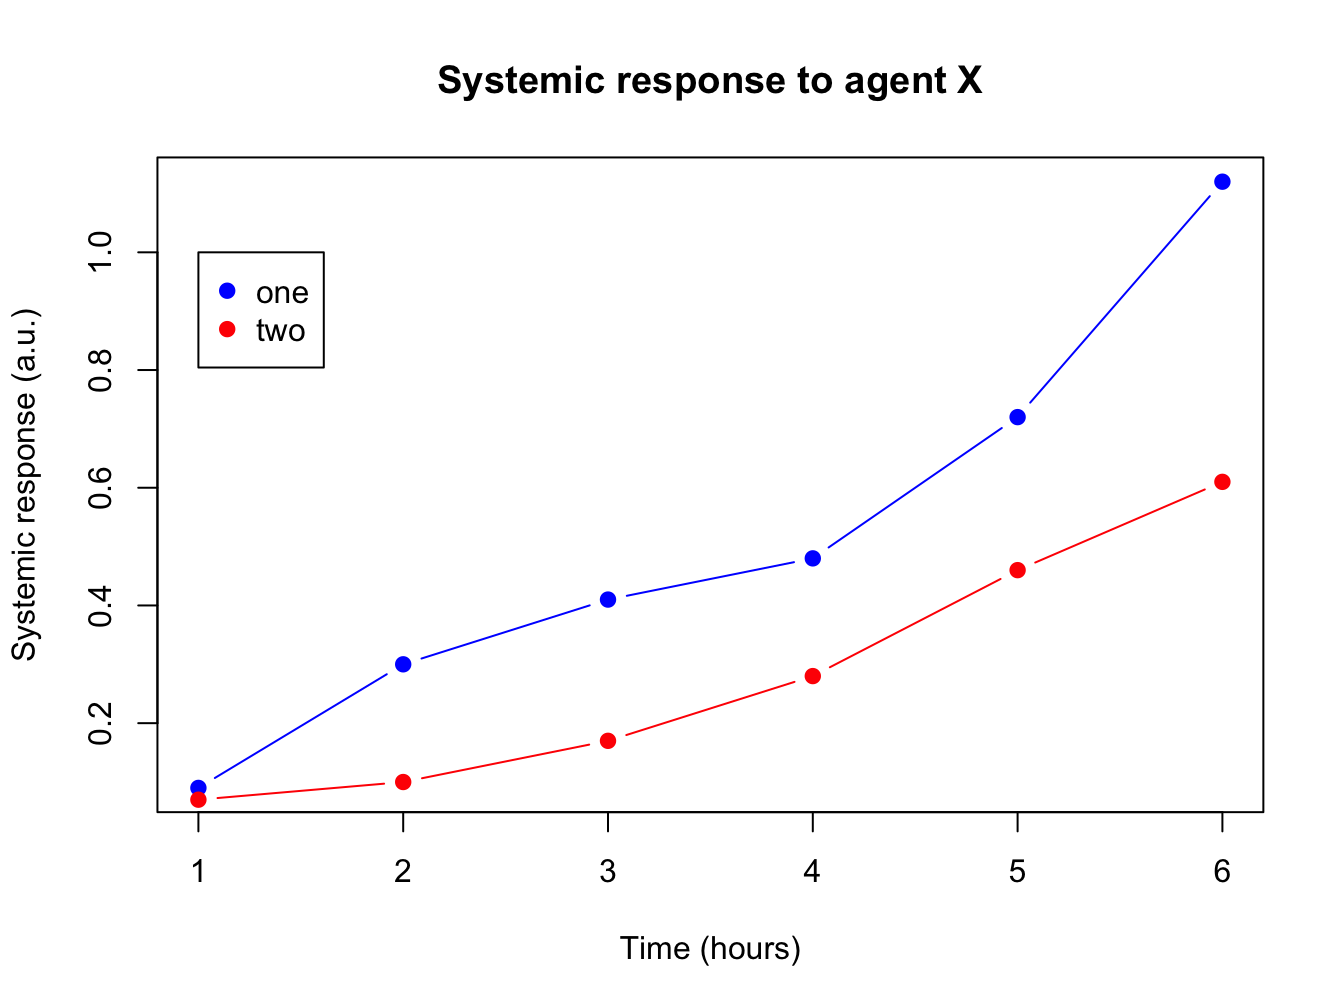
\includegraphics[width=0.8\linewidth]{davur_ebook_files/figure-latex/plot-legend-1-1} \end{center}

The \texttt{legend()} function is \emph{very} versatile. Have a look at the docs!
In its most basic form you pass it a position (x and y), series names, colors and plot character.

\hypertarget{helper-lines-and-lm}{%
\subsection{\texorpdfstring{Helper lines and \texttt{lm()}}{Helper lines and lm()}}\label{helper-lines-and-lm}}

Adding helper lines can be used to aid your reader in grasping and interpreting your data story.
Use the function \texttt{abline()} for this.

There are four types of helper lines you might want to add to a figure:

\begin{itemize}
\tightlist
\item
  A horizontal line with \texttt{h\ =}: indicate some y-threshold
\item
  A vertical line with \texttt{v\ =}: indicate x-threshold or mean or some other statistic
\item
  A line with an intercept (\texttt{a\ =}) and a slope (\texttt{b\ =}): often used to indicate some expected response, or diagonal x = y
\item
  A linear model, determined with the \texttt{lm()} function. The linear model object actually contains an intercept and a slope value which is taken by \texttt{abline()}.
\end{itemize}

In the following plot, these four basic helper lines are demonstrated:

\begin{Shaded}
\begin{Highlighting}[]
\KeywordTok{plot}\NormalTok{(}\DataTypeTok{x =}\NormalTok{ time, }\DataTypeTok{y =}\NormalTok{ response, }\DataTypeTok{pch =} \DecValTok{19}\NormalTok{, }\DataTypeTok{type =} \StringTok{"b"}\NormalTok{,}
     \DataTypeTok{xlab =} \StringTok{"Time (hours)"}\NormalTok{, }\DataTypeTok{ylab =} \StringTok{"Systemic response (a.u.)"}\NormalTok{,}
     \DataTypeTok{main =} \StringTok{"Systemic response to agent X"}\NormalTok{, }\DataTypeTok{col =} \StringTok{"blue"}\NormalTok{)}
\CommentTok{#horizontal line}
\KeywordTok{abline}\NormalTok{(}\DataTypeTok{h =} \FloatTok{0.3}\NormalTok{, }\DataTypeTok{lty =} \DecValTok{2}\NormalTok{, }\DataTypeTok{lwd =} \DecValTok{2}\NormalTok{, }\DataTypeTok{col =} \StringTok{"red"}\NormalTok{)}
\CommentTok{#vertical line}
\KeywordTok{abline}\NormalTok{(}\DataTypeTok{v =} \DecValTok{4}\NormalTok{, }\DataTypeTok{lty =} \DecValTok{3}\NormalTok{, }\DataTypeTok{lwd =} \DecValTok{2}\NormalTok{, }\DataTypeTok{col =} \StringTok{"darkgreen"}\NormalTok{)}
\CommentTok{#line with slope}
\KeywordTok{abline}\NormalTok{(}\DataTypeTok{a =} \FloatTok{-0.1}\NormalTok{, }\DataTypeTok{b =} \FloatTok{0.3}\NormalTok{, }\DataTypeTok{lwd =} \DecValTok{2}\NormalTok{, }\DataTypeTok{col =} \StringTok{"purple"}\NormalTok{)}
\CommentTok{#linear model }
\KeywordTok{abline}\NormalTok{(}\KeywordTok{lm}\NormalTok{(response }\OperatorTok{~}\StringTok{ }\NormalTok{time),  }\DataTypeTok{lwd =} \DecValTok{2}\NormalTok{, }\DataTypeTok{col =} \StringTok{"maroon"}\NormalTok{)}
\end{Highlighting}
\end{Shaded}

\begin{center}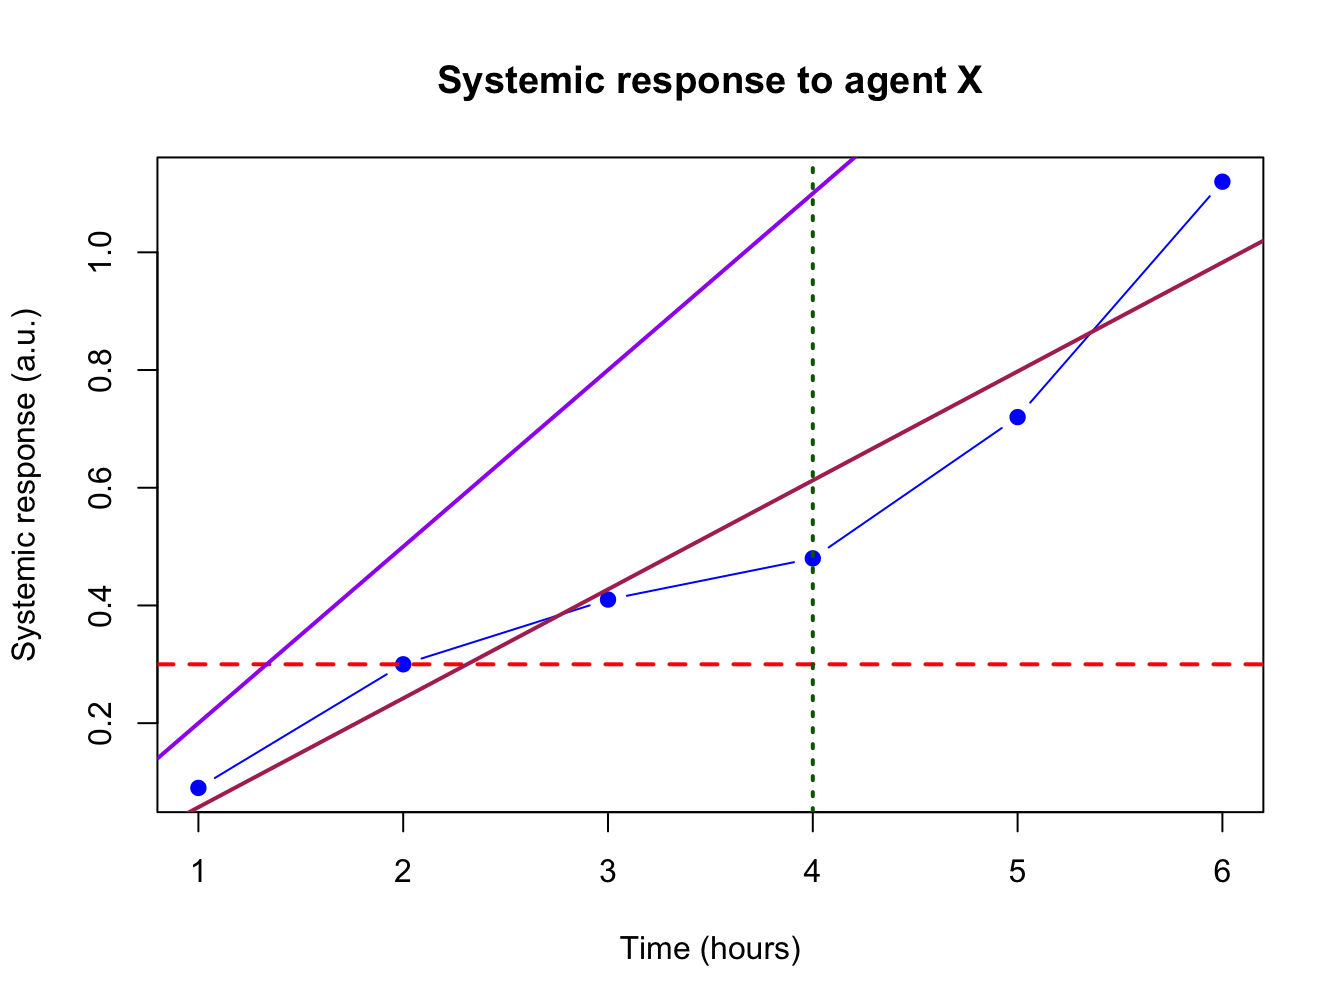
\includegraphics[width=0.8\linewidth]{davur_ebook_files/figure-latex/plot-helpers-1-1} \end{center}

\hypertarget{graphical-parameters-to-plot}{%
\section{\texorpdfstring{Graphical parameters to \texttt{plot()}}{Graphical parameters to plot()}}\label{graphical-parameters-to-plot}}

There are \emph{many} parameters that can be passed to the plotting functions. Here is a small sample and their possible values.

\begin{Shaded}
\begin{Highlighting}[]
\NormalTok{series <-}\StringTok{ }\DecValTok{1}\OperatorTok{:}\DecValTok{20}
\KeywordTok{plot}\NormalTok{(}\DecValTok{0}\NormalTok{, }\DecValTok{0}\NormalTok{, }\DataTypeTok{xlim=}\KeywordTok{c}\NormalTok{(}\DecValTok{1}\NormalTok{,}\DecValTok{20}\NormalTok{) , }\DataTypeTok{ylim=}\KeywordTok{c}\NormalTok{(}\FloatTok{0.5}\NormalTok{, }\FloatTok{7.5}\NormalTok{), }\DataTypeTok{col=}\StringTok{"white"}\NormalTok{ , }\DataTypeTok{yaxt=}\StringTok{"n"}\NormalTok{ , }\DataTypeTok{ylab=}\StringTok{""}\NormalTok{ , }\DataTypeTok{xlab=}\StringTok{""}\NormalTok{)}

\CommentTok{# the rainbow() function gives a nice palette across all colors}
\CommentTok{# or use hcl.colors() to specify another palette}
\CommentTok{# use  hcl.pals() to get an overview of available pallettes}
\NormalTok{colors =}\StringTok{ }\KeywordTok{hcl.colors}\NormalTok{(}\DecValTok{20}\NormalTok{, }\DataTypeTok{alpha =} \FloatTok{0.8}\NormalTok{, }\DataTypeTok{palette =} \StringTok{'viridis'}\NormalTok{)}

\CommentTok{#pch}
\KeywordTok{points}\NormalTok{(series, }\KeywordTok{rep}\NormalTok{(}\DecValTok{1}\NormalTok{, }\DecValTok{20}\NormalTok{), }\DataTypeTok{pch =} \DecValTok{1}\OperatorTok{:}\DecValTok{20}\NormalTok{, }\DataTypeTok{cex =} \DecValTok{2}\NormalTok{)}
\CommentTok{#col}
\KeywordTok{points}\NormalTok{(series, }\KeywordTok{rep}\NormalTok{(}\DecValTok{2}\NormalTok{, }\DecValTok{20}\NormalTok{), }\DataTypeTok{col =}\NormalTok{ colors, }\DataTypeTok{pch =} \DecValTok{16}\NormalTok{, }\DataTypeTok{cex =} \DecValTok{3}\NormalTok{)}
\CommentTok{#cex}
\KeywordTok{points}\NormalTok{(series, }\KeywordTok{rep}\NormalTok{(}\DecValTok{3}\NormalTok{, }\DecValTok{20}\NormalTok{), }\DataTypeTok{col =} \StringTok{"black"}\NormalTok{ , }\DataTypeTok{pch =} \DecValTok{16}\NormalTok{, }\DataTypeTok{cex =}\NormalTok{ series }\OperatorTok{*}\StringTok{ }\FloatTok{0.2}\NormalTok{)}

\CommentTok{#overlay to create new symbol}
\KeywordTok{points}\NormalTok{(series, }\KeywordTok{rep}\NormalTok{(}\DecValTok{4}\NormalTok{, }\DecValTok{20}\NormalTok{), }\DataTypeTok{pch =}\NormalTok{ series, }\DataTypeTok{cex =} \FloatTok{2.5}\NormalTok{, }\DataTypeTok{col =} \StringTok{"blue"}\NormalTok{)}
\KeywordTok{points}\NormalTok{(series, }\KeywordTok{rep}\NormalTok{(}\DecValTok{4}\NormalTok{, }\DecValTok{20}\NormalTok{), }\DataTypeTok{pch =}\NormalTok{ series, }\DataTypeTok{cex =} \FloatTok{1.5}\NormalTok{, }\DataTypeTok{col =}\NormalTok{ colors)}
 
\CommentTok{#lty}
\ControlFlowTok{for}\NormalTok{ (i }\ControlFlowTok{in} \DecValTok{1}\OperatorTok{:}\DecValTok{6}\NormalTok{) \{}
    \KeywordTok{points}\NormalTok{(}\KeywordTok{c}\NormalTok{(}\OperatorTok{-}\DecValTok{2}\NormalTok{, }\DecValTok{0}\NormalTok{) }\OperatorTok{+}\StringTok{ }\NormalTok{(i }\OperatorTok{*}\StringTok{ }\DecValTok{3}\NormalTok{), }\KeywordTok{c}\NormalTok{(}\DecValTok{5}\NormalTok{, }\DecValTok{5}\NormalTok{), }\DataTypeTok{col =} \StringTok{"black"}\NormalTok{, }\DataTypeTok{lty =}\NormalTok{ i, }\DataTypeTok{type =} \StringTok{"l"}\NormalTok{, }\DataTypeTok{lwd =} \DecValTok{3}\NormalTok{)}
    \KeywordTok{text}\NormalTok{((i }\OperatorTok{*}\StringTok{ }\DecValTok{3}\NormalTok{) }\OperatorTok{-}\StringTok{ }\DecValTok{1}\NormalTok{, }\FloatTok{5.25}\NormalTok{ , i)}
\NormalTok{\}}
\CommentTok{#type and lwd}
\ControlFlowTok{for}\NormalTok{ (i }\ControlFlowTok{in} \DecValTok{1}\OperatorTok{:}\DecValTok{4}\NormalTok{) \{}
    \CommentTok{#type}
    \KeywordTok{points}\NormalTok{(}\KeywordTok{c}\NormalTok{(}\OperatorTok{-}\DecValTok{4}\NormalTok{, }\DecValTok{-3}\NormalTok{, }\DecValTok{-2}\NormalTok{, }\DecValTok{-1}\NormalTok{) }\OperatorTok{+}\StringTok{ }\NormalTok{(i }\OperatorTok{*}\StringTok{ }\DecValTok{5}\NormalTok{), }\KeywordTok{rep}\NormalTok{(}\DecValTok{6}\NormalTok{, }\DecValTok{4}\NormalTok{),}
           \DataTypeTok{col =} \StringTok{"black"}\NormalTok{, }\DataTypeTok{type =} \KeywordTok{c}\NormalTok{(}\StringTok{"p"}\NormalTok{,}\StringTok{"l"}\NormalTok{,}\StringTok{"b"}\NormalTok{,}\StringTok{"o"}\NormalTok{)[i], }\DataTypeTok{lwd=}\DecValTok{2}\NormalTok{)}
    \KeywordTok{text}\NormalTok{((i }\OperatorTok{*}\StringTok{ }\DecValTok{5}\NormalTok{) }\OperatorTok{-}\StringTok{ }\FloatTok{2.5}\NormalTok{, }\FloatTok{6.4}\NormalTok{ , }\KeywordTok{c}\NormalTok{(}\StringTok{"p"}\NormalTok{,}\StringTok{"l"}\NormalTok{,}\StringTok{"b"}\NormalTok{,}\StringTok{"o"}\NormalTok{)[i] )}
    \CommentTok{#lwd}
    \KeywordTok{points}\NormalTok{(}\KeywordTok{c}\NormalTok{(}\OperatorTok{-}\DecValTok{4}\NormalTok{, }\DecValTok{-3}\NormalTok{, }\DecValTok{-2}\NormalTok{, }\DecValTok{-1}\NormalTok{) }\OperatorTok{+}\StringTok{ }\NormalTok{(i }\OperatorTok{*}\StringTok{ }\DecValTok{5}\NormalTok{), }\KeywordTok{rep}\NormalTok{(}\DecValTok{7}\NormalTok{, }\DecValTok{4}\NormalTok{), }\DataTypeTok{col =} \StringTok{"blue"}\NormalTok{, }\DataTypeTok{type =} \StringTok{"l"}\NormalTok{, }\DataTypeTok{lwd =}\NormalTok{ i)}
    \KeywordTok{text}\NormalTok{((i }\OperatorTok{*}\StringTok{ }\DecValTok{5}\NormalTok{) }\OperatorTok{-}\StringTok{ }\FloatTok{2.5}\NormalTok{, }\FloatTok{7.23}\NormalTok{, i)}
\NormalTok{\}}
\CommentTok{#add axis}
\KeywordTok{axis}\NormalTok{(}\DataTypeTok{side =} \DecValTok{2}\NormalTok{, }\DataTypeTok{at =} \KeywordTok{c}\NormalTok{(}\DecValTok{1}\NormalTok{, }\DecValTok{2}\NormalTok{, }\DecValTok{3}\NormalTok{, }\DecValTok{4}\NormalTok{, }\DecValTok{5}\NormalTok{, }\DecValTok{6}\NormalTok{, }\DecValTok{7}\NormalTok{),}
    \DataTypeTok{labels =} \KeywordTok{c}\NormalTok{(}\StringTok{"pch"}\NormalTok{ , }\StringTok{"col"}\NormalTok{ , }\StringTok{"cex"}\NormalTok{ , }\StringTok{"combine"}\NormalTok{, }\StringTok{"lty"}\NormalTok{, }\StringTok{"type"}\NormalTok{ , }\StringTok{"lwd"}\NormalTok{ ),}
    \DataTypeTok{tick =} \OtherTok{FALSE}\NormalTok{, }\DataTypeTok{col =} \StringTok{"black"}\NormalTok{, }\DataTypeTok{las =} \DecValTok{1}\NormalTok{, }\DataTypeTok{cex.axis =} \FloatTok{0.8}\NormalTok{)}
\end{Highlighting}
\end{Shaded}

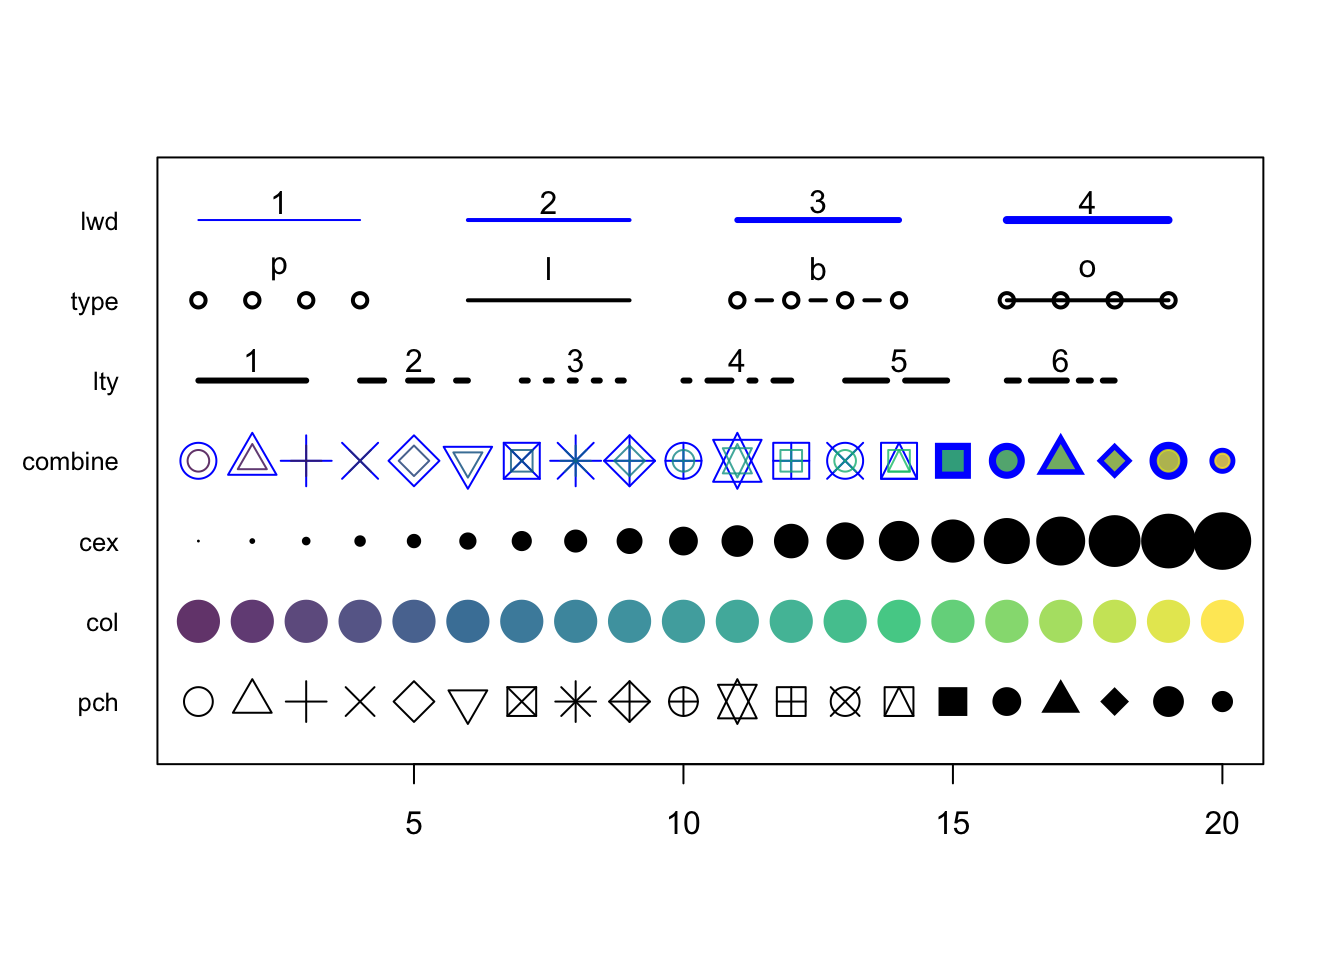
\includegraphics{davur_ebook_files/figure-latex/unnamed-chunk-14-1.pdf}

\hypertarget{complex-datatypes-and-file-reading}{%
\chapter{Complex Datatypes and File Reading}\label{complex-datatypes-and-file-reading}}

\hypertarget{matrices-are-vectors-with-dimensions}{%
\section{Matrices are vectors with dimensions}\label{matrices-are-vectors-with-dimensions}}

We will not detail on them in this course, only this one small paragraph. This does not mean they are not important, but they are just not the focus here. Some functions require or return a matrix so you should be aware of them.

\begin{Shaded}
\begin{Highlighting}[]
\NormalTok{m <-}\StringTok{ }\KeywordTok{matrix}\NormalTok{(}\DecValTok{1}\OperatorTok{:}\DecValTok{10}\NormalTok{, }\DataTypeTok{nrow =} \DecValTok{2}\NormalTok{, }\DataTypeTok{ncol =} \DecValTok{5}\NormalTok{) }
\NormalTok{m}
\end{Highlighting}
\end{Shaded}

\begin{verbatim}
##      [,1] [,2] [,3] [,4] [,5]
## [1,]    1    3    5    7    9
## [2,]    2    4    6    8   10
\end{verbatim}

\begin{Shaded}
\begin{Highlighting}[]
\NormalTok{v <-}\StringTok{ }\DecValTok{1}\OperatorTok{:}\DecValTok{10}
\KeywordTok{dim}\NormalTok{(v) <-}\StringTok{ }\KeywordTok{c}\NormalTok{(}\DecValTok{2}\NormalTok{, }\DecValTok{5}\NormalTok{)}
\NormalTok{v}
\end{Highlighting}
\end{Shaded}

\begin{verbatim}
##      [,1] [,2] [,3] [,4] [,5]
## [1,]    1    3    5    7    9
## [2,]    2    4    6    8   10
\end{verbatim}

\hypertarget{factors-nominal-ordinal-scales}{%
\section{Factors: Nominal \& Ordinal scales}\label{factors-nominal-ordinal-scales}}

Although factors are not actually a complex datatype but very much one of the five base types in R, I saved them because they have some more complex and sometimes puzzling behaviour.

\begin{quote}
Factors represent different discrete levels of a variable - the \emph{nominal} and \emph{ordinal} scales known from statistics.
\end{quote}

For instance:

\begin{itemize}
\tightlist
\item
  eye color (brown, blue, green)
\item
  weight class (underweight, normal, obese)
\item
  autism spectrum (none, minimal, heavy)
\end{itemize}

\hypertarget{factor-creation}{%
\subsubsection*{Factor creation}\label{factor-creation}}
\addcontentsline{toc}{subsubsection}{Factor creation}

Factors are used to represent data in nominal and ordinal scales. \textbf{\emph{Nominal}} has no order (e.g.~eye color). \textbf{\emph{Ordinal}} has order (e.g.~autism spectrum), but can not be calculated with, other than ordering from high to low. No \emph{distance} is defined between separate levels. The following functions are used to create factors:

\begin{itemize}
\tightlist
\item
  \texttt{factor()}: constructor function, from factor, character, numeric or logical
\item
  \texttt{as.factor()}: coercion function, from factor, character, numeric or logical
\item
  \texttt{cut()}: conversion function from numeric vector
\end{itemize}

So what is the difference between \texttt{factor()} and \texttt{as.factor()}? Function \texttt{as.factor()} is a \emph{wrapper} for \texttt{factor()}. The difference lies in behaviour when the input is a factor itself: \texttt{factor} will omit unused levels. Besides this, \texttt{as.factor()} does not specify the arguments for labels and levels.

\begin{Shaded}
\begin{Highlighting}[]
\NormalTok{x <-}\StringTok{ }\KeywordTok{factor}\NormalTok{(}\KeywordTok{c}\NormalTok{(}\StringTok{"a"}\NormalTok{, }\StringTok{"b"}\NormalTok{), }\DataTypeTok{levels =} \KeywordTok{c}\NormalTok{(}\StringTok{"a"}\NormalTok{, }\StringTok{"b"}\NormalTok{, }\StringTok{"c"}\NormalTok{))}
\NormalTok{x}
\KeywordTok{factor}\NormalTok{(x)}
\KeywordTok{as.factor}\NormalTok{(x)}
\end{Highlighting}
\end{Shaded}

\begin{verbatim}
## [1] a b
## Levels: a b c
## [1] a b
## Levels: a b
## [1] a b
## Levels: a b c
\end{verbatim}

Suppose you have surveyed the eye color of your class room and found these values

\begin{Shaded}
\begin{Highlighting}[]
\NormalTok{eye_colors <-}\StringTok{ }\KeywordTok{c}\NormalTok{(}\StringTok{"green"}\NormalTok{, }\StringTok{"blue"}\NormalTok{, }\StringTok{"brown"}\NormalTok{, }\StringTok{"brown"}\NormalTok{, }\StringTok{"blue"}\NormalTok{,}
    \StringTok{"brown"}\NormalTok{, }\StringTok{"brown"}\NormalTok{, }\StringTok{"brown"}\NormalTok{, }\StringTok{"blue"}\NormalTok{, }\StringTok{"brown"}\NormalTok{, }\StringTok{"green"}\NormalTok{,}
    \StringTok{"brown"}\NormalTok{, }\StringTok{"brown"}\NormalTok{, }\StringTok{"blue"}\NormalTok{, }\StringTok{"blue"}\NormalTok{, }\StringTok{"brown"}\NormalTok{)}
\end{Highlighting}
\end{Shaded}

Next you would like to plot or tabulate these findings. Simply plotting gives an error:

\begin{Shaded}
\begin{Highlighting}[]
\KeywordTok{plot}\NormalTok{(eye_colors)}
\end{Highlighting}
\end{Shaded}

\begin{verbatim}
## Warning in xy.coords(x, y, xlabel, ylabel, log): NAs introduced by coercion
\end{verbatim}

\begin{verbatim}
## Warning in min(x): no non-missing arguments to min; returning Inf
\end{verbatim}

\begin{verbatim}
## Warning in max(x): no non-missing arguments to max; returning -Inf
\end{verbatim}

\begin{verbatim}
## Error in plot.window(...): need finite 'ylim' values
\end{verbatim}

\begin{center}
\includegraphics[width=0.8\linewidth]{davur_ebook_files/figure-latex/eye-color-2-1} \end{center}

However, plotting a character vector converted to a factor is easy

\begin{Shaded}
\begin{Highlighting}[]
\NormalTok{eye_colors <-}\StringTok{ }\KeywordTok{as.factor}\NormalTok{(eye_colors)}
\KeywordTok{plot}\NormalTok{(eye_colors)}
\end{Highlighting}
\end{Shaded}

\begin{center}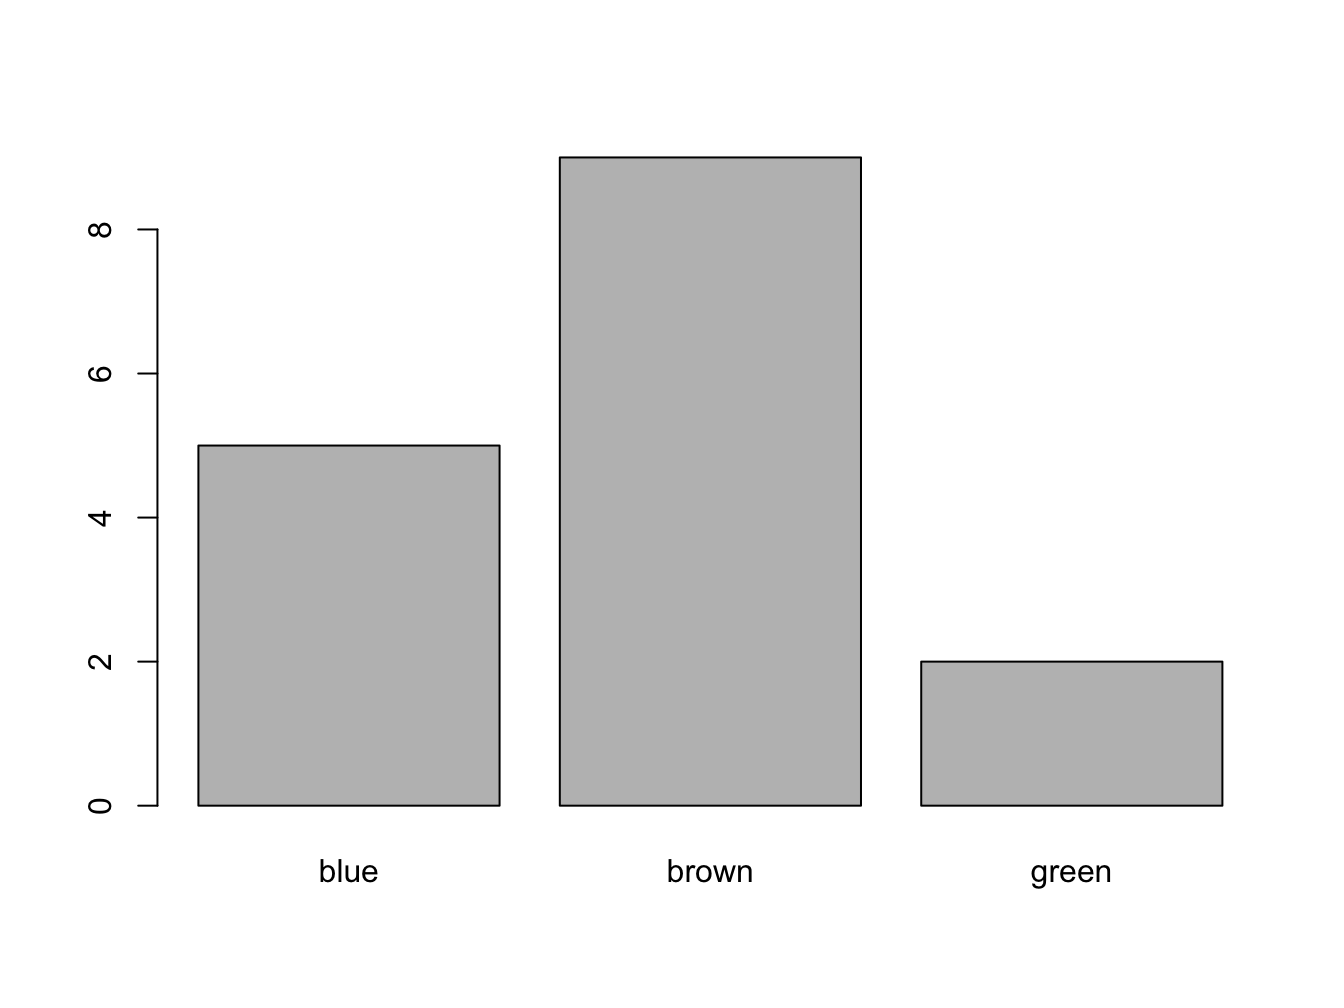
\includegraphics[width=0.8\linewidth]{davur_ebook_files/figure-latex/eye-color-3-1} \end{center}

Factors are also really easy to tabulate and filter

\begin{Shaded}
\begin{Highlighting}[]
\KeywordTok{table}\NormalTok{(eye_colors)}
\end{Highlighting}
\end{Shaded}

\begin{verbatim}
## eye_colors
##  blue brown green 
##     5     9     2
\end{verbatim}

\begin{Shaded}
\begin{Highlighting}[]
\KeywordTok{sum}\NormalTok{(eye_colors }\OperatorTok{==}\StringTok{ "blue"}\NormalTok{)}
\end{Highlighting}
\end{Shaded}

\begin{verbatim}
## [1] 5
\end{verbatim}

\hypertarget{levels-labels-and-ordering}{%
\subsubsection*{Levels, Labels and Ordering}\label{levels-labels-and-ordering}}
\addcontentsline{toc}{subsubsection}{Levels, Labels and Ordering}

When working with ordinal scales, defining the order of the factors (levels) is crucial. By default, R uses the \emph{natural ordering} which means it will stick to either numerical (\texttt{numeric}, \texttt{integer} and \texttt{logical}) or alphabetical ordering (\texttt{character}). When you want a different ordering you need to specify this. You can even define missing levels, as shown in the following example.

\begin{Shaded}
\begin{Highlighting}[]
\NormalTok{classSizes <-}\StringTok{ }\KeywordTok{factor}\NormalTok{(}\KeywordTok{c}\NormalTok{(}\StringTok{"big"}\NormalTok{, }\StringTok{"small"}\NormalTok{, }\StringTok{"huge"}\NormalTok{, }\StringTok{"huge"}\NormalTok{, }
    \StringTok{"small"}\NormalTok{,}\StringTok{"big"}\NormalTok{,}\StringTok{"small"}\NormalTok{,}\StringTok{"big"}\NormalTok{),}
    \DataTypeTok{levels =} \KeywordTok{c}\NormalTok{(}\StringTok{"small"}\NormalTok{, }\StringTok{"normal"}\NormalTok{, }\StringTok{"big"}\NormalTok{, }\StringTok{"huge"}\NormalTok{),}
    \DataTypeTok{ordered =} \OtherTok{TRUE}\NormalTok{) }\CommentTok{#make it an ordinal scale!}
\KeywordTok{plot}\NormalTok{(classSizes)}
\end{Highlighting}
\end{Shaded}

\begin{center}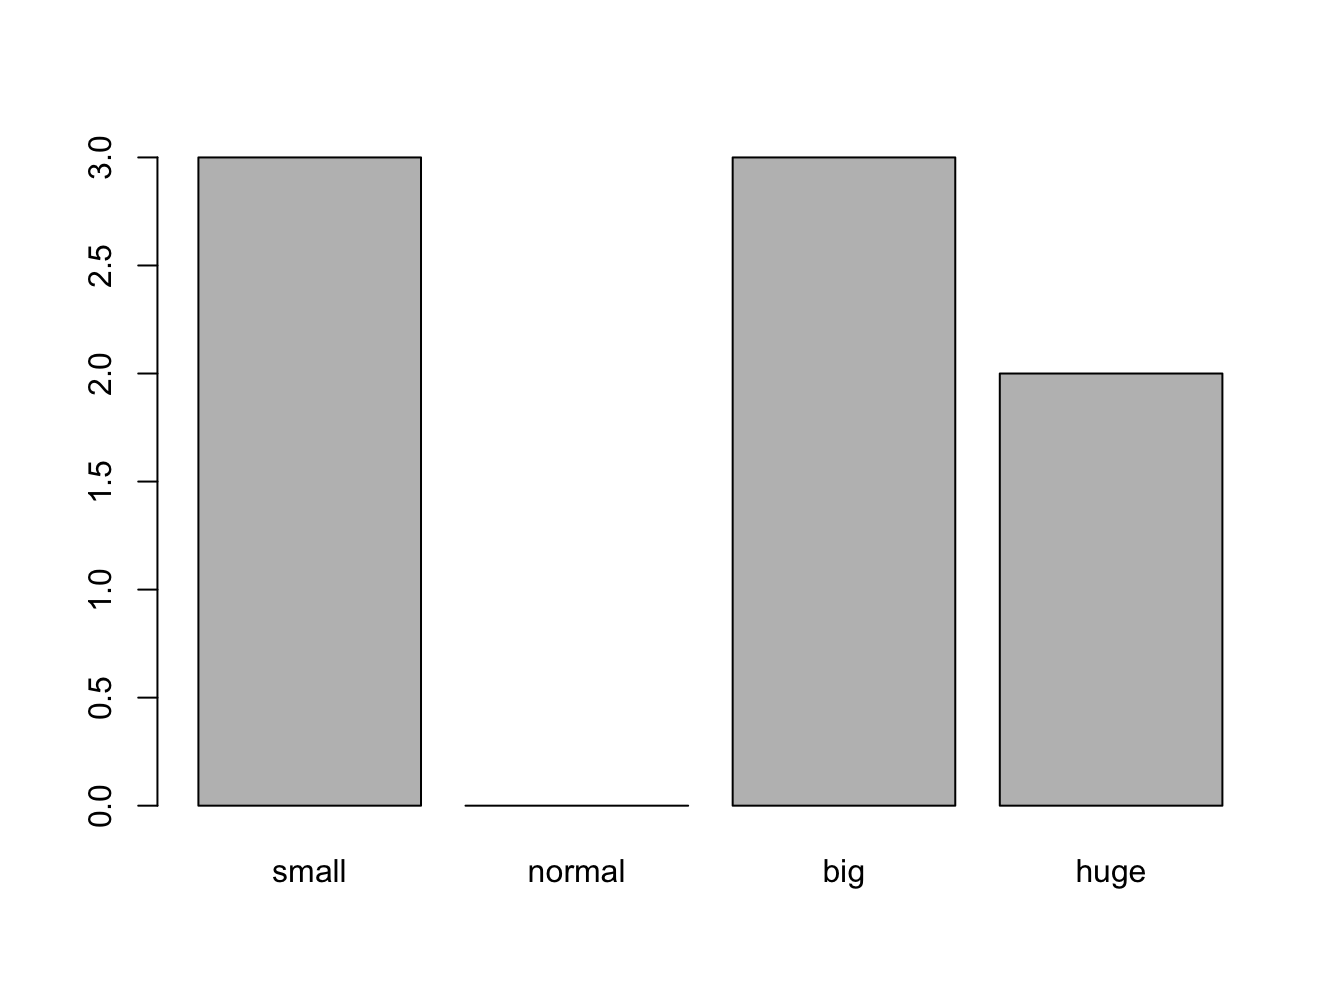
\includegraphics[width=0.8\linewidth]{davur_ebook_files/figure-latex/class-sizes-1-1} \end{center}

When you have factor, you can do a -limited- set of calulations with it. However, comparators only work with ordinal scale. As with all equality tests, \texttt{sum()} works as well:

\begin{Shaded}
\begin{Highlighting}[]
\NormalTok{classSizes }\OperatorTok{<}\StringTok{ "big"} \CommentTok{## only with in Ordinal scale}
\end{Highlighting}
\end{Shaded}

\begin{verbatim}
## [1] FALSE  TRUE FALSE FALSE  TRUE FALSE  TRUE FALSE
\end{verbatim}

\begin{Shaded}
\begin{Highlighting}[]
\KeywordTok{sum}\NormalTok{(classSizes }\OperatorTok{==}\StringTok{ "huge"}\NormalTok{) }
\end{Highlighting}
\end{Shaded}

\begin{verbatim}
## [1] 2
\end{verbatim}

\hypertarget{convert-existing-factors}{%
\subsubsection*{Convert existing factors}\label{convert-existing-factors}}
\addcontentsline{toc}{subsubsection}{Convert existing factors}

When you already have an unordered factor, you can make it ordered by using the function \texttt{ordered()} together with a fvector specifying the levels.

\begin{Shaded}
\begin{Highlighting}[]
\NormalTok{classSizes <-}\StringTok{ }\KeywordTok{factor}\NormalTok{(}\KeywordTok{c}\NormalTok{(}\StringTok{"big"}\NormalTok{, }\StringTok{"small"}\NormalTok{, }\StringTok{"huge"}\NormalTok{, }\StringTok{"huge"}\NormalTok{,}
    \StringTok{"small"}\NormalTok{, }\StringTok{"big"}\NormalTok{, }\StringTok{"small"}\NormalTok{, }\StringTok{"big"}\NormalTok{))}
\NormalTok{classSizes <-}\StringTok{ }\KeywordTok{ordered}\NormalTok{(classSizes,}
                    \DataTypeTok{levels =} \KeywordTok{c}\NormalTok{(}\StringTok{"small"}\NormalTok{, }\StringTok{"big"}\NormalTok{, }\StringTok{"huge"}\NormalTok{))}
\NormalTok{classSizes}
\end{Highlighting}
\end{Shaded}

\begin{verbatim}
## [1] big   small huge  huge  small big   small big  
## Levels: small < big < huge
\end{verbatim}

\hypertarget{when-calculations-get-corrupted}{%
\subsubsection*{When calculations get corrupted}\label{when-calculations-get-corrupted}}
\addcontentsline{toc}{subsubsection}{When calculations get corrupted}

Especially when a factor consists of numeric levels, calculations can get your mind screwed big time:

\begin{Shaded}
\begin{Highlighting}[]
\NormalTok{x <-}\StringTok{ }\KeywordTok{factor}\NormalTok{(}\KeywordTok{c}\NormalTok{(}\DecValTok{3}\NormalTok{, }\DecValTok{4}\NormalTok{, }\DecValTok{5}\NormalTok{, }\DecValTok{4}\NormalTok{))}
\NormalTok{x }\OperatorTok{+}\StringTok{ }\DecValTok{1}
\end{Highlighting}
\end{Shaded}

\begin{verbatim}
## Warning in Ops.factor(x, 1): '+' not meaningful for factors
\end{verbatim}

\begin{verbatim}
## [1] NA NA NA NA
\end{verbatim}

\begin{Shaded}
\begin{Highlighting}[]
\KeywordTok{as.integer}\NormalTok{(x) }\OperatorTok{+}\StringTok{ }\DecValTok{1}
\end{Highlighting}
\end{Shaded}

\begin{verbatim}
## [1] 2 3 4 3
\end{verbatim}

\begin{Shaded}
\begin{Highlighting}[]
\KeywordTok{as.integer}\NormalTok{(}\KeywordTok{levels}\NormalTok{(x)) }\OperatorTok{+}\StringTok{ }\DecValTok{1}
\end{Highlighting}
\end{Shaded}

\begin{verbatim}
## [1] 4 5 6
\end{verbatim}

The only way to get the numbers back with numeric factors is by using this trick

\begin{Shaded}
\begin{Highlighting}[]
\NormalTok{x}
\end{Highlighting}
\end{Shaded}

\begin{verbatim}
## [1] 3 4 5 4
## Levels: 3 4 5
\end{verbatim}

\begin{Shaded}
\begin{Highlighting}[]
\KeywordTok{as.integer}\NormalTok{(}\KeywordTok{levels}\NormalTok{(x))[x]}
\end{Highlighting}
\end{Shaded}

\begin{verbatim}
## [1] 3 4 5 4
\end{verbatim}

But this makes for really unintelligible code so try to prevent this at all costs!

\hypertarget{the-power-of-factors}{%
\subsubsection*{The power of factors}\label{the-power-of-factors}}
\addcontentsline{toc}{subsubsection}{The power of factors}

Factors are used all the time e.g.~for defining treated/untreated. That's why R knows how to deal with them so well:

\begin{Shaded}
\begin{Highlighting}[]
\KeywordTok{with}\NormalTok{(ChickWeight, }\KeywordTok{plot}\NormalTok{(weight }\OperatorTok{~}\StringTok{ }\NormalTok{Diet))}
\end{Highlighting}
\end{Shaded}

\begin{center}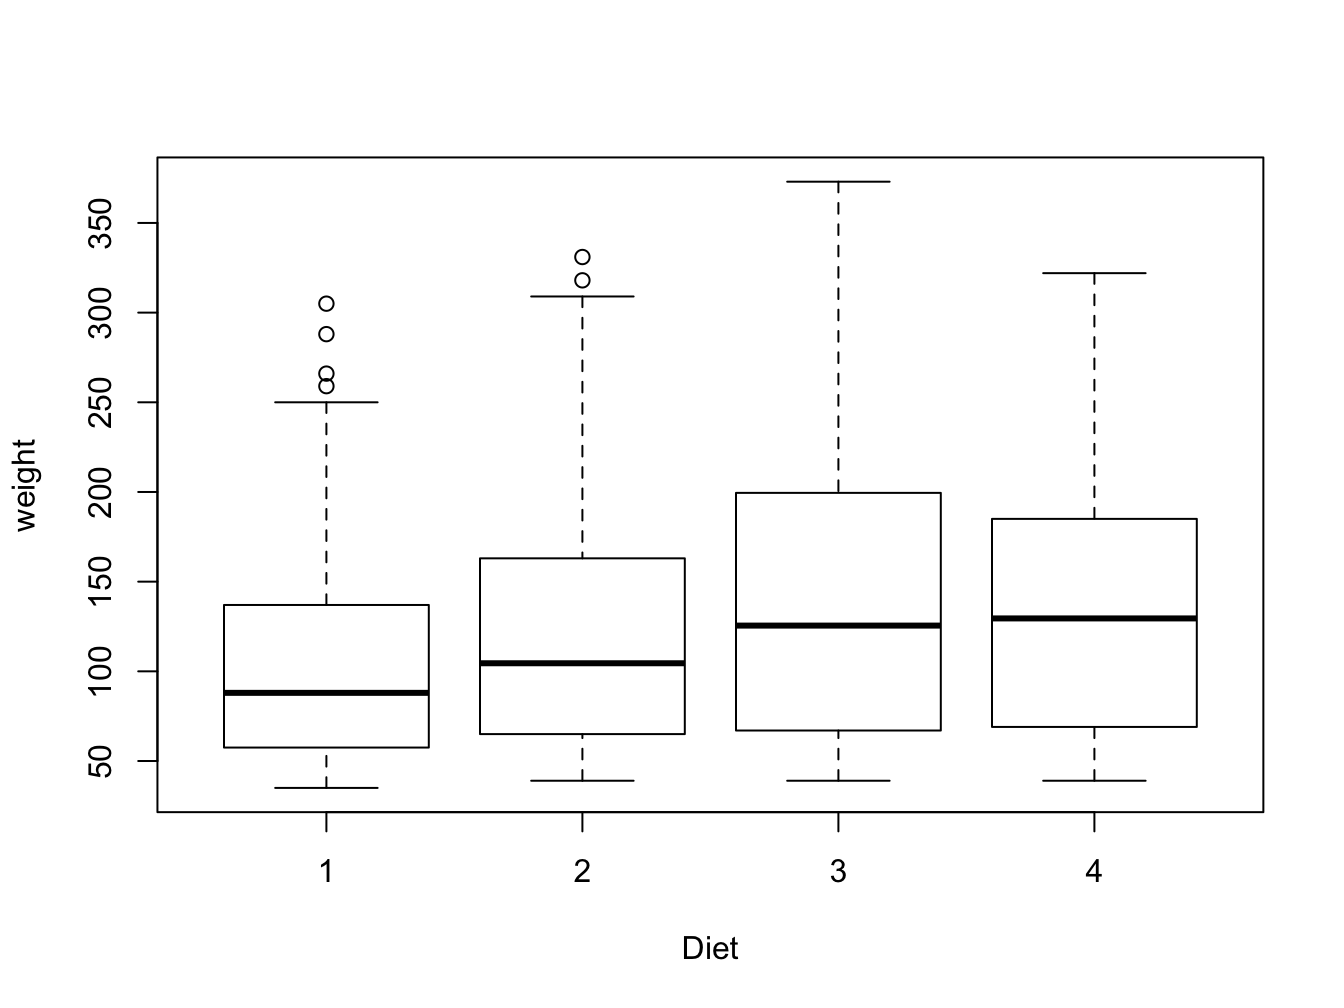
\includegraphics[width=0.8\linewidth]{davur_ebook_files/figure-latex/factor-plotting-1} \end{center}

You will see many many exaples in the subsequent chapters of this and the next course.

\hypertarget{lists}{%
\section{Lists}\label{lists}}

\begin{quote}
A list is an \textbf{\emph{ordered collection of vectors}}. These vectors can have \emph{differing types} and \emph{differing lengths}.
\end{quote}

\hypertarget{list-creation}{%
\subsubsection*{List creation}\label{list-creation}}
\addcontentsline{toc}{subsubsection}{List creation}

Create a list with or without element names:

\begin{itemize}
\tightlist
\item
  \texttt{list(element1,\ element2,\ ...)}~\\
\item
  \texttt{list(name1\ =\ element1,\ name2\ =\ element2,\ ...)}
\end{itemize}

Without names:

\begin{Shaded}
\begin{Highlighting}[]
\NormalTok{x <-}\StringTok{ }\KeywordTok{c}\NormalTok{(}\DecValTok{2}\NormalTok{, }\DecValTok{3}\NormalTok{, }\DecValTok{1}\NormalTok{);  y <-}\StringTok{ }\KeywordTok{c}\NormalTok{(}\StringTok{"foo"}\NormalTok{, }\StringTok{"bar"}\NormalTok{)}
\NormalTok{l <-}\StringTok{ }\KeywordTok{list}\NormalTok{(x, y); l}
\end{Highlighting}
\end{Shaded}

\begin{verbatim}
## [[1]]
## [1] 2 3 1
## 
## [[2]]
## [1] "foo" "bar"
\end{verbatim}

\begin{Shaded}
\begin{Highlighting}[]
\NormalTok{l[[}\DecValTok{2}\NormalTok{]]}
\end{Highlighting}
\end{Shaded}

\begin{verbatim}
## [1] "foo" "bar"
\end{verbatim}

With names:

\begin{Shaded}
\begin{Highlighting}[]
\NormalTok{x <-}\StringTok{ }\KeywordTok{c}\NormalTok{(}\DecValTok{2}\NormalTok{, }\DecValTok{3}\NormalTok{, }\DecValTok{1}\NormalTok{)}
\NormalTok{y <-}\StringTok{ }\KeywordTok{c}\NormalTok{(}\StringTok{"foo"}\NormalTok{, }\StringTok{"bar"}\NormalTok{)}
\NormalTok{l <-}\StringTok{ }\KeywordTok{list}\NormalTok{(}\StringTok{"numbers"}\NormalTok{ =}\StringTok{ }\NormalTok{x, }\StringTok{"words"}\NormalTok{ =}\StringTok{ }\NormalTok{y)}
\NormalTok{l}
\end{Highlighting}
\end{Shaded}

\begin{verbatim}
## $numbers
## [1] 2 3 1
## 
## $words
## [1] "foo" "bar"
\end{verbatim}

This is the preferred way to create and use them because it gives you more and easier ways to access its elements and it makes for much more reradable code. That's why you will only see lists with named elements from here on.

\hypertarget{making-selections-on-lists}{%
\subsubsection*{Making selections on lists}\label{making-selections-on-lists}}
\addcontentsline{toc}{subsubsection}{Making selections on lists}

Accessing named elements can be done in three ways:

\begin{itemize}
\tightlist
\item
  By index, within double or single brackets: \texttt{{[}{[}\textless{}index\textgreater{}{]}{]}} or \texttt{{[}\textless{}index\textgreater{}{]}}
\item
  By name of the element, within double or single brackets: \texttt{{[}{[}\textless{}name\textgreater{}{]}{]}} or \texttt{{[}\textless{}name\textgreater{}{]}}
\item
  By name of the element, using the dollar sign on the list name: \texttt{\$\textless{}name\textgreater{}}
\end{itemize}

Here are all three:

\begin{Shaded}
\begin{Highlighting}[]
\NormalTok{l[[}\DecValTok{2}\NormalTok{]]        }\CommentTok{# index}
\end{Highlighting}
\end{Shaded}

\begin{verbatim}
## [1] "foo" "bar"
\end{verbatim}

\begin{Shaded}
\begin{Highlighting}[]
\NormalTok{l[[}\StringTok{"words"}\NormalTok{]]  }\CommentTok{# name of element with double brackets}
\end{Highlighting}
\end{Shaded}

\begin{verbatim}
## [1] "foo" "bar"
\end{verbatim}

\begin{Shaded}
\begin{Highlighting}[]
\NormalTok{l}\OperatorTok{$}\NormalTok{words       }\CommentTok{# name of element with dollar sign}
\end{Highlighting}
\end{Shaded}

\begin{verbatim}
## [1] "foo" "bar"
\end{verbatim}

\begin{quote}
Single brackets selection on a list returns a list; double brackets and \texttt{\$} return a vector.
\end{quote}

\begin{Shaded}
\begin{Highlighting}[]
\NormalTok{l[}\DecValTok{2}\NormalTok{]}
\end{Highlighting}
\end{Shaded}

\begin{verbatim}
## $words
## [1] "foo" "bar"
\end{verbatim}

\begin{Shaded}
\begin{Highlighting}[]
\NormalTok{l[[}\DecValTok{2}\NormalTok{]]}
\end{Highlighting}
\end{Shaded}

\begin{verbatim}
## [1] "foo" "bar"
\end{verbatim}

\begin{Shaded}
\begin{Highlighting}[]
\NormalTok{l}\OperatorTok{$}\NormalTok{words}
\end{Highlighting}
\end{Shaded}

\begin{verbatim}
## [1] "foo" "bar"
\end{verbatim}

In R, selections are often \textbf{\emph{chained}}. In the following example the second vector element of the second list element is selected.

\begin{Shaded}
\begin{Highlighting}[]
\NormalTok{l}
\NormalTok{l[[}\DecValTok{2}\NormalTok{]][}\DecValTok{2}\NormalTok{] }
\end{Highlighting}
\end{Shaded}

\begin{verbatim}
## $numbers
## [1] 2 3 1
## 
## $words
## [1] "foo" "bar"
## 
## [1] "bar"
\end{verbatim}

When you need multiple elements of a list, use \textbf{\emph{single brackets}}. Remember: single brackets return a list; that's why you need single brackets here.

\begin{Shaded}
\begin{Highlighting}[]
\NormalTok{l[}\KeywordTok{c}\NormalTok{(}\DecValTok{1}\NormalTok{,}\DecValTok{2}\NormalTok{,}\DecValTok{1}\NormalTok{)]}
\end{Highlighting}
\end{Shaded}

\begin{verbatim}
## $numbers
## [1] 2 3 1
## 
## $words
## [1] "foo" "bar"
## 
## $numbers
## [1] 2 3 1
\end{verbatim}

Accessing named elements has its limitations. You can not use a variable in combination with the dollar sign selector.

\begin{Shaded}
\begin{Highlighting}[]
\NormalTok{select <-}\StringTok{ "words"}
\NormalTok{l[[select]] }\CommentTok{## OK}
\end{Highlighting}
\end{Shaded}

\begin{verbatim}
## [1] "foo" "bar"
\end{verbatim}

\begin{Shaded}
\begin{Highlighting}[]
\NormalTok{l}\OperatorTok{$}\NormalTok{select }\CommentTok{##fails - no element with name "select"}
\end{Highlighting}
\end{Shaded}

\begin{verbatim}
## NULL
\end{verbatim}

Chaining of selectors can become awkward, as this example demonstrates.

\begin{Shaded}
\begin{Highlighting}[]
\NormalTok{l[}\DecValTok{2}\NormalTok{][}\StringTok{"words"}\NormalTok{][}\DecValTok{1}\NormalTok{]}\OperatorTok{$}\NormalTok{words  }\CommentTok{## mind****}
\end{Highlighting}
\end{Shaded}

\begin{verbatim}
## [1] "foo" "bar"
\end{verbatim}

\hypertarget{dataframes}{%
\section{Dataframes}\label{dataframes}}

\begin{quote}
A dataframe is an \textbf{\emph{ordered collection of vectors}}. These vectors can have \emph{differing types} but must have \emph{equal lengths}.
\end{quote}

A dataframe is very similar to the square grid-like structures you have probably worked with in Excel. Variables are in columns in which all elements are of the same type. Examples (observations) are in rows - they \emph{can} have differing types.

Dataframes can be constructed using the \texttt{data.frame()} function in the same way as the \texttt{list} function:\\
\texttt{data.frame(column1\ =\ vector1,\ column2\ =\ vector2,\ ...)}

Here is a first example.

\begin{Shaded}
\begin{Highlighting}[]
\NormalTok{geneNames <-}\StringTok{ }\KeywordTok{c}\NormalTok{(}\StringTok{"P53"}\NormalTok{,}\StringTok{"BRCA1"}\NormalTok{,}\StringTok{"VAMP1"}\NormalTok{, }\StringTok{"FHIT"}\NormalTok{)}
\NormalTok{sig <-}\StringTok{ }\KeywordTok{c}\NormalTok{(}\OtherTok{TRUE}\NormalTok{, }\OtherTok{TRUE}\NormalTok{, }\OtherTok{FALSE}\NormalTok{, }\OtherTok{FALSE}\NormalTok{)}
\NormalTok{meanExp <-}\StringTok{ }\KeywordTok{c}\NormalTok{(}\FloatTok{4.5}\NormalTok{, }\FloatTok{7.3}\NormalTok{, }\FloatTok{5.4}\NormalTok{, }\FloatTok{2.4}\NormalTok{)}
\NormalTok{genes <-}\StringTok{ }\KeywordTok{data.frame}\NormalTok{(}
    \StringTok{"name"}\NormalTok{ =}\StringTok{ }\NormalTok{geneNames,  }
    \StringTok{"significant"}\NormalTok{ =}\StringTok{ }\NormalTok{sig,  }
    \StringTok{"expression"}\NormalTok{ =}\StringTok{ }\NormalTok{meanExp)  }
\NormalTok{genes}
\end{Highlighting}
\end{Shaded}

\begin{verbatim}
##    name significant expression
## 1   P53        TRUE        4.5
## 2 BRCA1        TRUE        7.3
## 3 VAMP1       FALSE        5.4
## 4  FHIT       FALSE        2.4
\end{verbatim}

Here you can see the structure of a dataframe: each column has a single datatype but rows can have differing types for neighboring fields.

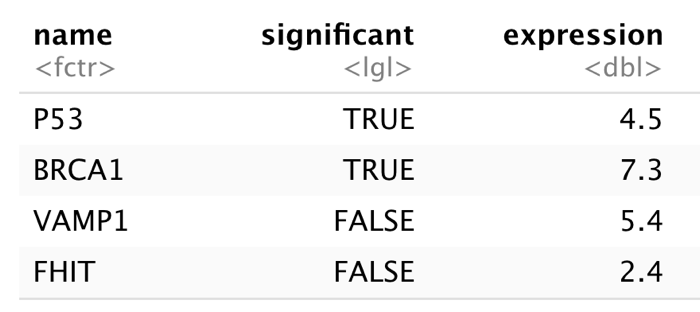
\includegraphics{figures/Dataframe_view1.png}

\hypertarget{selections-on-dataframes}{%
\subsection{Selections on dataframes}\label{selections-on-dataframes}}

Making selections on dataframes is not very surprising when you already know how to do it with vectors and lists. There is only one extension. The fact that it is a square grid-like structure makes it possible to add an extra way of making selections: combining rows and column selections as subgrids. This section extensively reviews all means of making selections.

This is a summary:

\begin{itemize}
\tightlist
\item
  Select a single column using \texttt{\$} will return a vector
\item
  Selecting with double brackets \texttt{{[}{[}\textless{}name\textgreater{}{]}{]}} or \texttt{{[}{[}\textless{}index\textgreater{}{]}{]}} will return a vector
\item
  Selecting with single brackets \texttt{{[}\textless{}name\textgreater{}{]}} or \texttt{{[}\textless{}index\textgreater{}{]}} will return a dataframe
\item
  Selecting with row-and-column coordinates \texttt{{[}row\_selection,\ col\_selection{]}} returns either a vector or a dataframe, depending on the selection made. Here, \texttt{row\_selection} and \texttt{col\_selection} can be

  \begin{itemize}
  \tightlist
  \item
    a numerical vector of length 1 or more
  \item
    a logical vector of length 1 or more
  \item
    empty (to select all rows/columns)
  \end{itemize}
\end{itemize}

Here follow a few examples.

\begin{Shaded}
\begin{Highlighting}[]
\OperatorTok{>}\StringTok{ }\NormalTok{genes[}\DecValTok{2}\NormalTok{,}\DecValTok{1}\NormalTok{]            }\CommentTok{#row 2, column 1}
\end{Highlighting}
\end{Shaded}

\begin{verbatim}
## [1] BRCA1
## Levels: BRCA1 FHIT P53 VAMP1
\end{verbatim}

\begin{Shaded}
\begin{Highlighting}[]
\OperatorTok{>}\StringTok{ }\NormalTok{genes[}\DecValTok{2}\NormalTok{, }\DecValTok{1}\OperatorTok{:}\DecValTok{2}\NormalTok{]     }\CommentTok{#row 2, columns 1 and 2}
\end{Highlighting}
\end{Shaded}

\begin{verbatim}
##    name significant
## 2 BRCA1        TRUE
\end{verbatim}

\begin{Shaded}
\begin{Highlighting}[]
\OperatorTok{>}\StringTok{ }\NormalTok{genes[}\DecValTok{2}\NormalTok{, }\KeywordTok{c}\NormalTok{(}\DecValTok{1}\NormalTok{, }\DecValTok{3}\NormalTok{)] }\CommentTok{#row 2, column 1 and 3}
\end{Highlighting}
\end{Shaded}

\begin{verbatim}
##    name expression
## 2 BRCA1        7.3
\end{verbatim}

\begin{Shaded}
\begin{Highlighting}[]
\OperatorTok{>}\StringTok{ }\NormalTok{genes}\OperatorTok{$}\NormalTok{name          }\CommentTok{#column "name"}
\end{Highlighting}
\end{Shaded}

\begin{verbatim}
## [1] P53   BRCA1 VAMP1 FHIT 
## Levels: BRCA1 FHIT P53 VAMP1
\end{verbatim}

\begin{Shaded}
\begin{Highlighting}[]
\OperatorTok{>}\StringTok{ }\NormalTok{genes[, }\KeywordTok{c}\NormalTok{(}\StringTok{"name"}\NormalTok{, }\StringTok{"expression"}\NormalTok{)]  }\CommentTok{#columns "name" and "expression", all rows}
\end{Highlighting}
\end{Shaded}

\begin{verbatim}
##    name expression
## 1   P53        4.5
## 2 BRCA1        7.3
## 3 VAMP1        5.4
## 4  FHIT        2.4
\end{verbatim}

\begin{Shaded}
\begin{Highlighting}[]
\OperatorTok{>}\StringTok{ }\NormalTok{genes[, }\DecValTok{1}\OperatorTok{:}\DecValTok{2}\NormalTok{]      }\CommentTok{#columns 1 and 2, all rows}
\end{Highlighting}
\end{Shaded}

\begin{verbatim}
##    name significant
## 1   P53        TRUE
## 2 BRCA1        TRUE
## 3 VAMP1       FALSE
## 4  FHIT       FALSE
\end{verbatim}

\begin{Shaded}
\begin{Highlighting}[]
\OperatorTok{>}\StringTok{ }\NormalTok{genes[}\DecValTok{1}\OperatorTok{:}\DecValTok{2}\NormalTok{, ]      }\CommentTok{#row 1 and 2, all columns}
\end{Highlighting}
\end{Shaded}

\begin{verbatim}
##    name significant expression
## 1   P53        TRUE        4.5
## 2 BRCA1        TRUE        7.3
\end{verbatim}

As with vectors and lists, R will cycle selectors, and you can select an element as often as you want.

\begin{Shaded}
\begin{Highlighting}[]
\NormalTok{genes[}\KeywordTok{c}\NormalTok{(T, F), }\DecValTok{1}\NormalTok{]   }\CommentTok{#every uneven row, column 1}
\end{Highlighting}
\end{Shaded}

\begin{verbatim}
## [1] P53   VAMP1
## Levels: BRCA1 FHIT P53 VAMP1
\end{verbatim}

\begin{Shaded}
\begin{Highlighting}[]
\NormalTok{genes[}\KeywordTok{c}\NormalTok{(}\DecValTok{1}\NormalTok{, }\DecValTok{1}\NormalTok{, }\DecValTok{1}\NormalTok{, }\DecValTok{2}\NormalTok{), ]  }\CommentTok{#three times row 1 and row 2}
\end{Highlighting}
\end{Shaded}

\begin{verbatim}
##      name significant expression
## 1     P53        TRUE        4.5
## 1.1   P53        TRUE        4.5
## 1.2   P53        TRUE        4.5
## 2   BRCA1        TRUE        7.3
\end{verbatim}

A dataframe is much like a list, but not entirely equal:

\begin{Shaded}
\begin{Highlighting}[]
\NormalTok{genes[[}\StringTok{"name"}\NormalTok{]] }\CommentTok{## select column w. double brackets}
\end{Highlighting}
\end{Shaded}

\begin{verbatim}
## [1] P53   BRCA1 VAMP1 FHIT 
## Levels: BRCA1 FHIT P53 VAMP1
\end{verbatim}

\begin{Shaded}
\begin{Highlighting}[]
\KeywordTok{class}\NormalTok{(genes) }\CommentTok{## it is NOT a list though}
\end{Highlighting}
\end{Shaded}

\begin{verbatim}
## [1] "data.frame"
\end{verbatim}

\begin{Shaded}
\begin{Highlighting}[]
\KeywordTok{str}\NormalTok{(genes)}
\end{Highlighting}
\end{Shaded}

\begin{verbatim}
## 'data.frame':    4 obs. of  3 variables:
##  $ name       : Factor w/ 4 levels "BRCA1","FHIT",..: 3 1 4 2
##  $ significant: logi  TRUE TRUE FALSE FALSE
##  $ expression : num  4.5 7.3 5.4 2.4
\end{verbatim}

\hypertarget{selections-with-subset}{%
\subsubsection*{\texorpdfstring{Selections with \texttt{subset()}}{Selections with subset()}}\label{selections-with-subset}}
\addcontentsline{toc}{subsubsection}{Selections with \texttt{subset()}}

Function \texttt{subset()} can serve as alternative to ``bracket-based'' selections (\texttt{{[}\ ,\ {]}}).
You can use \texttt{subset()} to make both \textbf{column} and \textbf{row selections}. Here, using \texttt{subset\ =}, the rows are selected for which Solar.R is available using the \texttt{is.na()} function.

\begin{Shaded}
\begin{Highlighting}[]
\KeywordTok{head}\NormalTok{(}\KeywordTok{subset}\NormalTok{(airquality, }\DataTypeTok{subset =} \OperatorTok{!}\KeywordTok{is.na}\NormalTok{(Solar.R)))}
\end{Highlighting}
\end{Shaded}

\begin{verbatim}
##   Ozone Solar.R Wind Temp Month Day
## 1    41     190  7.4   67   May   1
## 2    36     118  8.0   72   May   2
## 3    12     149 12.6   74   May   3
## 4    18     313 11.5   62   May   4
## 7    23     299  8.6   65   May   7
## 8    19      99 13.8   59   May   8
\end{verbatim}

Note that you don't even need to use quotes for column names.

Select columns only with the \texttt{select\ =} argument.

\begin{Shaded}
\begin{Highlighting}[]
\KeywordTok{head}\NormalTok{(}\KeywordTok{subset}\NormalTok{(airquality, }\DataTypeTok{select =} \KeywordTok{c}\NormalTok{(Ozone, Solar.R)))}
\end{Highlighting}
\end{Shaded}

\begin{verbatim}
##   Ozone Solar.R
## 1    41     190
## 2    36     118
## 3    12     149
## 4    18     313
## 5    NA      NA
## 6    28      NA
\end{verbatim}

Of course, you can combine row and colum selection:

\begin{Shaded}
\begin{Highlighting}[]
\KeywordTok{head}\NormalTok{(}\KeywordTok{subset}\NormalTok{(airquality, }
            \DataTypeTok{subset =} \OperatorTok{!}\KeywordTok{is.na}\NormalTok{(Solar.R), }
            \DataTypeTok{select =} \KeywordTok{c}\NormalTok{(Ozone, Solar.R)))}
\end{Highlighting}
\end{Shaded}

\begin{verbatim}
##   Ozone Solar.R
## 1    41     190
## 2    36     118
## 3    12     149
## 4    18     313
## 7    23     299
## 8    19      99
\end{verbatim}

\begin{Shaded}
\begin{Highlighting}[]
\CommentTok{# shorthand notation}
\CommentTok{#subset(airquality, Day == 1, select = -Temp)}
\end{Highlighting}
\end{Shaded}

\texttt{subset()} can be used more sophisticated; however we are going to see \texttt{subset()} on steroids in the next course: the functions in package \texttt{dplyr}.

\hypertarget{read-from-file-using-read.table}{%
\subsection{\texorpdfstring{Read from file using \texttt{read.table()}}{Read from file using read.table()}}\label{read-from-file-using-read.table}}

Usually your data comes from file, loaded into memory as a dataframe. The most common data transfer \& storage format is text. The text will have column separators that can be any of a whole number of characters, but tab- or comma-delimited are most common.\\
Here is an example dataset in a file (``whale\_selenium.txt'') where the separator is a space character:

\begin{verbatim}
whale liver.Se tooth.Se  
1 6.23 140.16  
2 6.79 133.32  
3 7.92 135.34  
...  
19 41.23 206.30  
20 45.47 141.31  
\end{verbatim}

To load this data into an R session you can use the function \texttt{read.table()}. Let's try

\begin{Shaded}
\begin{Highlighting}[]
\OperatorTok{>}\StringTok{ }\NormalTok{whale_selenium <-}\StringTok{ }\KeywordTok{read.table}\NormalTok{(}\StringTok{"data/whale_selenium.txt"}\NormalTok{)}
\OperatorTok{>}\StringTok{ }\KeywordTok{head}\NormalTok{(whale_selenium) }\CommentTok{# first rows}
\end{Highlighting}
\end{Shaded}

\begin{verbatim}
##      V1       V2       V3
## 1 whale liver.Se tooth.Se
## 2     1     6.23   140.16
## 3     2     6.79   133.32
## 4     3     7.92   135.34
## 5     4     8.02   127.82
## 6     5     9.34   108.67
\end{verbatim}

\begin{Shaded}
\begin{Highlighting}[]
\OperatorTok{>}\StringTok{ }\KeywordTok{str}\NormalTok{(whale_selenium) }\CommentTok{# structure}
\end{Highlighting}
\end{Shaded}

\begin{verbatim}
## 'data.frame':    21 obs. of  3 variables:
##  $ V1: Factor w/ 21 levels "1","10","11",..: 21 1 12 14 15 16 17 18 19 20 ...
##  $ V2: Factor w/ 21 levels "10.00","10.57",..: 21 16 17 18 19 20 1 2 3 4 ...
##  $ V3: Factor w/ 21 levels "108.67","112.63",..: 21 8 5 6 3 1 12 4 11 14 ...
\end{verbatim}

That is not entirely correct: all columns are imported as a factor while obviously they should be numeric. The cause of this is that, when loading the data,

\begin{itemize}
\tightlist
\item
  there is no special consideration for the header line
\item
  the separator is assumed to be a space
\item
  the decimal is assumed to be a dot ``.''
\end{itemize}

(and some more assumptions)

Therefore, to read a file correctly, you have to specify its format in every detail. in this case,

\begin{itemize}
\tightlist
\item
  the first line is a header with column names
\item
  the first column contains the row names
\end{itemize}

Here is a new attempt with some \textbf{\emph{format specifications}}:

\begin{Shaded}
\begin{Highlighting}[]
\NormalTok{whale_selenium <-}\StringTok{ }\KeywordTok{read.table}\NormalTok{(}
    \DataTypeTok{file =} \StringTok{"data/whale_selenium.txt"}\NormalTok{,}
    \DataTypeTok{header =} \OtherTok{TRUE}\NormalTok{,}
    \DataTypeTok{row.names =} \DecValTok{1}\NormalTok{)}
\end{Highlighting}
\end{Shaded}

Before proceeding with your data, you should always perform some checks. Several helper methods exist for this purpose:

\begin{itemize}
\tightlist
\item
  \texttt{head()} shows you the first \texttt{n} lines
\item
  \texttt{str()} gives you a structure description: what types have the columns and what dimension does the data frame have?
\item
  \texttt{summary()} gives you a 6-number sumary of the data
\end{itemize}

\begin{Shaded}
\begin{Highlighting}[]
\OperatorTok{>}\StringTok{ }\KeywordTok{head}\NormalTok{(whale_selenium, }\DataTypeTok{n=}\DecValTok{4}\NormalTok{) }
\end{Highlighting}
\end{Shaded}

\begin{verbatim}
##   liver.Se tooth.Se
## 1     6.23      140
## 2     6.79      133
## 3     7.92      135
## 4     8.02      128
\end{verbatim}

\begin{Shaded}
\begin{Highlighting}[]
\OperatorTok{>}\StringTok{ }\KeywordTok{str}\NormalTok{(whale_selenium) }
\end{Highlighting}
\end{Shaded}

\begin{verbatim}
## 'data.frame':    20 obs. of  2 variables:
##  $ liver.Se: num  6.23 6.79 7.92 8.02 9.34 ...
##  $ tooth.Se: num  140 133 135 128 109 ...
\end{verbatim}

\begin{Shaded}
\begin{Highlighting}[]
\OperatorTok{>}\StringTok{ }\KeywordTok{summary}\NormalTok{(whale_selenium) }
\end{Highlighting}
\end{Shaded}

\begin{verbatim}
##     liver.Se       tooth.Se  
##  Min.   : 6.2   Min.   :109  
##  1st Qu.: 9.8   1st Qu.:135  
##  Median :14.9   Median :143  
##  Mean   :20.7   Mean   :157  
##  3rd Qu.:33.6   3rd Qu.:175  
##  Max.   :45.5   Max.   :245
\end{verbatim}

There are various other helper methods the you can use to inspect the contents and nature of your dataframe columns and rows:

\begin{itemize}
\tightlist
\item
  \texttt{dim()} gives the rows and columns
\item
  \texttt{ncol()} gives the number of columns
\item
  \texttt{nrow()} gives the number of rows
\item
  \texttt{names()} gives the column names (synonym to \texttt{colnames()})
\item
  \texttt{rownames()} gives the row names
\end{itemize}

But visualizing your data speaks more than a thousand words of course.

\begin{Shaded}
\begin{Highlighting}[]
\KeywordTok{plot}\NormalTok{(whale_selenium}\OperatorTok{$}\NormalTok{liver.Se, whale_selenium}\OperatorTok{$}\NormalTok{tooth.Se,}
    \DataTypeTok{xlab =} \StringTok{"liver Selenium"}\NormalTok{, }\DataTypeTok{ylab =} \StringTok{"tooth Selenium"}\NormalTok{)}
\KeywordTok{abline}\NormalTok{(}\KeywordTok{lm}\NormalTok{(whale_selenium}\OperatorTok{$}\NormalTok{tooth.Se }\OperatorTok{~}\StringTok{ }\NormalTok{whale_selenium}\OperatorTok{$}\NormalTok{liver.Se))}
\end{Highlighting}
\end{Shaded}

\begin{center}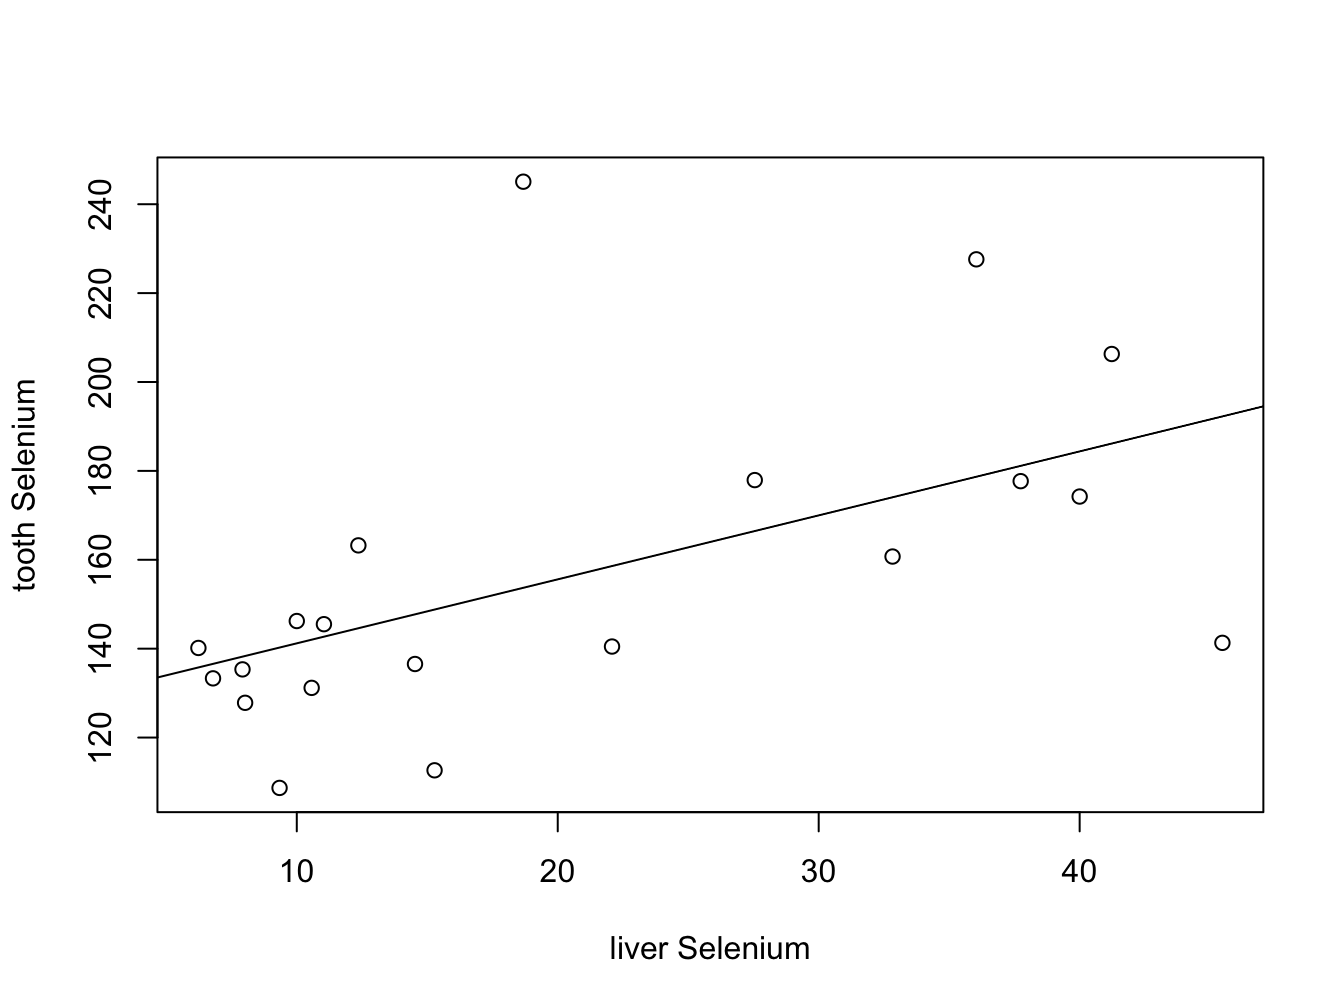
\includegraphics[width=0.8\linewidth]{davur_ebook_files/figure-latex/data-frame-io3-1} \end{center}

This is absolutely not the whole filereading story! The topic will be addressed again in a later chapter.

\hypertarget{dataframe-manipulations}{%
\subsection{Dataframe manipulations}\label{dataframe-manipulations}}

\hypertarget{changing-column-names}{%
\subsubsection*{Changing column names}\label{changing-column-names}}
\addcontentsline{toc}{subsubsection}{Changing column names}

Sometimes the existing column names are not convenient to work with (unclear, too long etc.). In that case it may be a good idea to change the column names. To do this you can use either \texttt{names()} or \texttt{colnames()}.

\begin{Shaded}
\begin{Highlighting}[]
\KeywordTok{names}\NormalTok{(whale_selenium) <-}\StringTok{ }\KeywordTok{c}\NormalTok{(}\StringTok{"liver"}\NormalTok{, }\StringTok{"tooth"}\NormalTok{)}
\KeywordTok{head}\NormalTok{(whale_selenium, }\DataTypeTok{n=}\DecValTok{2}\NormalTok{)}
\end{Highlighting}
\end{Shaded}

\begin{verbatim}
##   liver tooth
## 1  6.23   140
## 2  6.79   133
\end{verbatim}

\begin{Shaded}
\begin{Highlighting}[]
\CommentTok{##or}
\KeywordTok{colnames}\NormalTok{(whale_selenium) <-}\StringTok{ }\KeywordTok{c}\NormalTok{(}\StringTok{"pancreas"}\NormalTok{, }\StringTok{"colon"}\NormalTok{)}
\KeywordTok{head}\NormalTok{(whale_selenium, }\DataTypeTok{n=}\DecValTok{2}\NormalTok{)}
\end{Highlighting}
\end{Shaded}

\begin{verbatim}
##   pancreas colon
## 1     6.23   140
## 2     6.79   133
\end{verbatim}

\hypertarget{adding-columns}{%
\subsubsection*{Adding columns}\label{adding-columns}}
\addcontentsline{toc}{subsubsection}{Adding columns}

You can add a single column by simply specifying its name and the value(s) to be attached.

\begin{Shaded}
\begin{Highlighting}[]
\CommentTok{## add simulated stomach data}
\NormalTok{whale_selenium}\OperatorTok{$}\NormalTok{stomach <-}\StringTok{ }\KeywordTok{rnorm}\NormalTok{(}\KeywordTok{nrow}\NormalTok{(whale_selenium), }\DecValTok{42}\NormalTok{, }\DecValTok{6}\NormalTok{) }
\KeywordTok{head}\NormalTok{(whale_selenium, }\DataTypeTok{n=}\DecValTok{2}\NormalTok{)}
\end{Highlighting}
\end{Shaded}

\begin{verbatim}
##   liver tooth stomach
## 1  6.23   140    52.5
## 2  6.79   133    50.7
\end{verbatim}

Alternatively, use \texttt{cbind}. It is a bit more versatile because you can add multiple columns at once.

\begin{Shaded}
\begin{Highlighting}[]
\KeywordTok{cbind}\NormalTok{(whale_selenium, }\StringTok{"brain"}\NormalTok{ =}\StringTok{ }\KeywordTok{c}\NormalTok{(}\DecValTok{1}\NormalTok{, }\DecValTok{0}\NormalTok{)) }\CommentTok{#cycled values!}
\end{Highlighting}
\end{Shaded}

\begin{verbatim}
##    liver tooth stomach brain
## 1   6.23   140    52.5     1
## 2   6.79   133    50.7     0
## 3   7.92   135    39.3     1
## 4   8.02   128    42.8     0
## 5   9.34   109    39.8     1
## 6  10.00   146    34.8     0
## 7  10.57   131    26.0     1
## 8  11.04   146    41.8     0
## 9  12.36   163    41.8     1
## 10 14.53   137    51.9     0
## 11 15.28   113    30.0     1
## 12 18.68   245    38.0     0
## 13 22.08   140    47.3     1
## 14 27.55   178    44.1     0
## 15 32.83   161    42.7     1
## 16 36.04   228    38.3     0
## 17 37.74   178    43.2     1
## 18 40.00   174    40.6     0
## 19 41.23   206    42.7     1
## 20 45.47   141    38.5     0
\end{verbatim}

\hypertarget{adding-rows-rbind}{%
\subsubsection*{\texorpdfstring{Adding rows: \texttt{rbind()}}{Adding rows: rbind()}}\label{adding-rows-rbind}}
\addcontentsline{toc}{subsubsection}{Adding rows: \texttt{rbind()}}

Adding rows to a dataframe is similar. There is however a constraint: the column names of both dataframes need to match for this operation to succeed.

\begin{Shaded}
\begin{Highlighting}[]
\NormalTok{my_data1 <-}\StringTok{ }\KeywordTok{data.frame}\NormalTok{(}\DataTypeTok{colA =} \DecValTok{1}\OperatorTok{:}\DecValTok{3}\NormalTok{, }\DataTypeTok{colB =} \KeywordTok{c}\NormalTok{(}\StringTok{"a"}\NormalTok{, }\StringTok{"b"}\NormalTok{, }\StringTok{"c"}\NormalTok{))}
\NormalTok{my_data2 <-}\StringTok{ }\KeywordTok{data.frame}\NormalTok{(}\DataTypeTok{colA =} \DecValTok{4}\OperatorTok{:}\DecValTok{5}\NormalTok{, }\DataTypeTok{colB =} \KeywordTok{c}\NormalTok{(}\StringTok{"d"}\NormalTok{, }\StringTok{"e"}\NormalTok{))}
\NormalTok{my_data_complete <-}\StringTok{ }\KeywordTok{rbind}\NormalTok{(my_data1, my_data2)}
\NormalTok{my_data_complete}
\end{Highlighting}
\end{Shaded}

\begin{verbatim}
##   colA colB
## 1    1    a
## 2    2    b
## 3    3    c
## 4    4    d
## 5    5    e
\end{verbatim}

\hypertarget{functions-1}{%
\chapter{Functions}\label{functions-1}}

\hypertarget{dealing-with-nas}{%
\section{Dealing with NAs}\label{dealing-with-nas}}

Dealing with NA is a \textbf{\emph{very big thing}}. When you work with external data there is always the possibility that some values will be missing.

You should be aware that it is not possible to test for \texttt{NA} values (Not Available) values in any other way; using \texttt{==} will simply return \texttt{NA}:

\begin{Shaded}
\begin{Highlighting}[]
\NormalTok{x <-}\StringTok{ }\OtherTok{NA}
\NormalTok{x }\OperatorTok{==}\StringTok{ }\OtherTok{NA}
\end{Highlighting}
\end{Shaded}

\begin{verbatim}
## [1] NA
\end{verbatim}

Other important functions for dealing with that are \texttt{na.omit()} and \texttt{complete.cases()}. Besides that, many functions in R have a (variant of) the \texttt{na.rm\ =} argument. For instance, when the \texttt{sum()} function encounters an NA in its input vector, it will always return \texttt{NA}:

\begin{Shaded}
\begin{Highlighting}[]
\NormalTok{x <-}\StringTok{ }\KeywordTok{c}\NormalTok{(}\DecValTok{1}\NormalTok{, }\DecValTok{2}\NormalTok{, }\DecValTok{3}\NormalTok{, }\OtherTok{NA}\NormalTok{)}
\KeywordTok{sum}\NormalTok{(x)}
\end{Highlighting}
\end{Shaded}

\begin{verbatim}
## [1] NA
\end{verbatim}

\begin{Shaded}
\begin{Highlighting}[]
\KeywordTok{sum}\NormalTok{(x, }\DataTypeTok{na.rm =} \OtherTok{TRUE}\NormalTok{)}
\end{Highlighting}
\end{Shaded}

\begin{verbatim}
## [1] 6
\end{verbatim}

\hypertarget{descriptive-statistics}{%
\section{Descriptive statistics}\label{descriptive-statistics}}

R provides a wealth of descriptive statistics functions. The most important ones of them are listed below. The ones with an asterisk are described in more detail in following paragraphs.

\begin{longtable}[]{@{}ll@{}}
\toprule
function & purpose\tabularnewline
\midrule
\endhead
\texttt{mean(\ )} & mean\tabularnewline
\texttt{median(\ )} & median\tabularnewline
\texttt{min(\ )} & minimum\tabularnewline
\texttt{max(\ )} & maximum\tabularnewline
\texttt{range(\ )} & min and max\tabularnewline
\texttt{var(\ )} & variance s\^{}2\tabularnewline
\texttt{sd(\ )} & standard deviation s\tabularnewline
\texttt{summary(\ )} & 6-number summary\tabularnewline
\texttt{quantile(\ )} * & quantiles\tabularnewline
\texttt{IQR(\ )} * & interquantile range\tabularnewline
\bottomrule
\end{longtable}

\hypertarget{the-quantile-function}{%
\subsubsection*{\texorpdfstring{The \texttt{quantile()} function}{The quantile() function}}\label{the-quantile-function}}
\addcontentsline{toc}{subsubsection}{The \texttt{quantile()} function}

This function gives the data values corresponding to the specified quantiles. The function defaults to the quantiles \texttt{0\%\ \ 25\%\ \ 50\%\ \ 75\%\ 100\%}: these are the \emph{quartiles} of course.

\begin{Shaded}
\begin{Highlighting}[]
\KeywordTok{quantile}\NormalTok{(ChickWeight}\OperatorTok{$}\NormalTok{weight)}
\end{Highlighting}
\end{Shaded}

\begin{verbatim}
##   0%  25%  50%  75% 100% 
##   35   63  103  164  373
\end{verbatim}

\begin{Shaded}
\begin{Highlighting}[]
\KeywordTok{quantile}\NormalTok{(ChickWeight}\OperatorTok{$}\NormalTok{weight, }\DataTypeTok{probs =} \KeywordTok{seq}\NormalTok{(}\DecValTok{0}\NormalTok{, }\DecValTok{1}\NormalTok{, }\FloatTok{0.2}\NormalTok{))}
\end{Highlighting}
\end{Shaded}

\begin{verbatim}
##   0%  20%  40%  60%  80% 100% 
##   35   57   85  126  182  373
\end{verbatim}

\hypertarget{interquantile-range-iqr}{%
\subsubsection*{\texorpdfstring{Interquantile range \texttt{IQR()}}{Interquantile range IQR()}}\label{interquantile-range-iqr}}
\addcontentsline{toc}{subsubsection}{Interquantile range \texttt{IQR()}}

Function \texttt{IQR()} gives the range between the 25\% and 75\% quantiles.

\begin{Shaded}
\begin{Highlighting}[]
\KeywordTok{IQR}\NormalTok{(ChickWeight}\OperatorTok{$}\NormalTok{weight)}
\end{Highlighting}
\end{Shaded}

\begin{verbatim}
## [1] 101
\end{verbatim}

\begin{Shaded}
\begin{Highlighting}[]
\CommentTok{## same as}
\KeywordTok{quantile}\NormalTok{(ChickWeight}\OperatorTok{$}\NormalTok{weight)[}\DecValTok{4}\NormalTok{] }\OperatorTok{-}\StringTok{ }\KeywordTok{quantile}\NormalTok{(ChickWeight}\OperatorTok{$}\NormalTok{weight)[}\DecValTok{2}\NormalTok{]}
\end{Highlighting}
\end{Shaded}

\begin{verbatim}
## 75% 
## 101
\end{verbatim}

\begin{Shaded}
\begin{Highlighting}[]
\CommentTok{## same as}
\KeywordTok{diff}\NormalTok{(}\KeywordTok{quantile}\NormalTok{(ChickWeight}\OperatorTok{$}\NormalTok{weight, }\DataTypeTok{probs =} \KeywordTok{c}\NormalTok{(}\FloatTok{0.25}\NormalTok{, }\FloatTok{0.75}\NormalTok{)))}
\end{Highlighting}
\end{Shaded}

\begin{verbatim}
## 75% 
## 101
\end{verbatim}

\hypertarget{boxplot-is-summary-visualized}{%
\subsubsection*{\texorpdfstring{\texttt{boxplot()} is \texttt{summary()} visualized}{boxplot() is summary() visualized}}\label{boxplot-is-summary-visualized}}
\addcontentsline{toc}{subsubsection}{\texttt{boxplot()} is \texttt{summary()} visualized}

Boxplot is a graph of the 5-number summary, but \texttt{summary()} also gives the mean

\begin{Shaded}
\begin{Highlighting}[]
\KeywordTok{summary}\NormalTok{(ChickWeight}\OperatorTok{$}\NormalTok{weight)}
\end{Highlighting}
\end{Shaded}

\begin{verbatim}
##    Min. 1st Qu.  Median    Mean 3rd Qu.    Max. 
##      35      63     103     122     164     373
\end{verbatim}

\begin{Shaded}
\begin{Highlighting}[]
\KeywordTok{boxplot}\NormalTok{(ChickWeight}\OperatorTok{$}\NormalTok{weight)}
\end{Highlighting}
\end{Shaded}

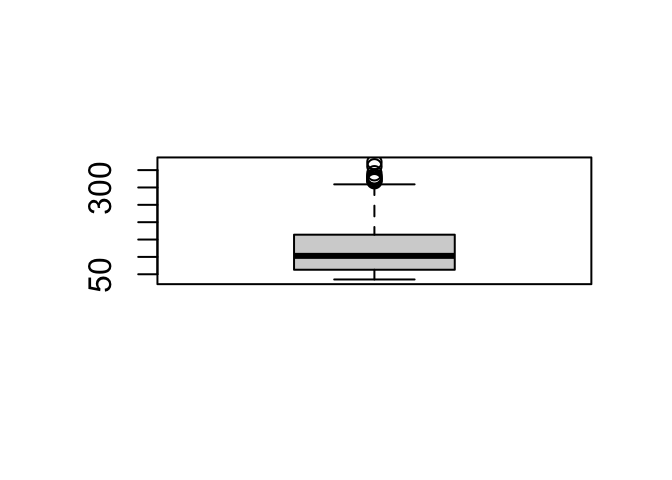
\includegraphics{davur_ebook_files/figure-latex/box_demo-1.pdf}

\hypertarget{general-purpose-functions}{%
\section{General purpose functions}\label{general-purpose-functions}}

\hypertarget{memory-management}{%
\subsubsection*{Memory management}\label{memory-management}}
\addcontentsline{toc}{subsubsection}{Memory management}

When working with large datasets it may be useful to free some memory once in a while (i.e.~intermediate results). Use \texttt{ls()} to see what is in memory; use \texttt{rm()} to delete single or several items: \texttt{rm(genes)}, \texttt{rm(x,\ y,\ z)} and clear all by typing \texttt{rm(list\ =\ ls())}

\hypertarget{file-system-operations}{%
\subsubsection*{File system operations}\label{file-system-operations}}
\addcontentsline{toc}{subsubsection}{File system operations}

Several functions exist for working with the file system:

\begin{itemize}
\tightlist
\item
  \texttt{getwd()} returns the current working directory.
\item
  \texttt{setwd(\textless{}/path/to/folder\textgreater{})} sets the current working directory.
\item
  \texttt{dir()}, \texttt{dir(path)} lists the contents of the current directory, or of \texttt{path}.
\item
  A \texttt{path} can be defined as \texttt{"E:\textbackslash{}\textbackslash{}emile\textbackslash{}\textbackslash{}datasets"} (Windows) or, on Linux/Mac using relative paths \texttt{"\textasciitilde{}/datasets"} or absolute paths \texttt{"/home/emile/datasets"}.
\end{itemize}

\hypertarget{glueing-character-elements-paste}{%
\subsubsection*{\texorpdfstring{Glueing character elements: \texttt{paste()}}{Glueing character elements: paste()}}\label{glueing-character-elements-paste}}
\addcontentsline{toc}{subsubsection}{Glueing character elements: \texttt{paste()}}

Use \texttt{paste()} to combine elements into a string

\begin{Shaded}
\begin{Highlighting}[]
\KeywordTok{paste}\NormalTok{(}\DecValTok{1}\NormalTok{, }\DecValTok{2}\NormalTok{, }\DecValTok{3}\NormalTok{)}
\end{Highlighting}
\end{Shaded}

\begin{verbatim}
## [1] "1 2 3"
\end{verbatim}

\begin{Shaded}
\begin{Highlighting}[]
\KeywordTok{paste}\NormalTok{(}\DecValTok{1}\NormalTok{, }\DecValTok{2}\NormalTok{, }\DecValTok{3}\NormalTok{, }\DataTypeTok{sep=}\StringTok{"-"}\NormalTok{)}
\end{Highlighting}
\end{Shaded}

\begin{verbatim}
## [1] "1-2-3"
\end{verbatim}

\begin{Shaded}
\begin{Highlighting}[]
\KeywordTok{paste}\NormalTok{(}\DecValTok{1}\OperatorTok{:}\DecValTok{12}\NormalTok{, month.abb)}
\end{Highlighting}
\end{Shaded}

\begin{verbatim}
##  [1] "1 Jan"  "2 Feb"  "3 Mar"  "4 Apr"  "5 May"  "6 Jun"  "7 Jul" 
##  [8] "8 Aug"  "9 Sep"  "10 Oct" "11 Nov" "12 Dec"
\end{verbatim}

There is a variant, \texttt{paste0()} which uses no separator by default.

\hypertarget{a-local-namespace-with}{%
\subsubsection*{\texorpdfstring{A local namespace: \texttt{with()}}{A local namespace: with()}}\label{a-local-namespace-with}}
\addcontentsline{toc}{subsubsection}{A local namespace: \texttt{with()}}

When you have a piece of related code operating on a single dataset, use \texttt{with()} so you don't have to type its name all the time.

\begin{Shaded}
\begin{Highlighting}[]
\KeywordTok{with}\NormalTok{(airquality, \{}
\NormalTok{  mdl <-}\StringTok{ }\KeywordTok{lm}\NormalTok{(Solar.R }\OperatorTok{~}\StringTok{ }\NormalTok{Temp)}
  \KeywordTok{plot}\NormalTok{(Solar.R }\OperatorTok{~}\StringTok{ }\NormalTok{Temp)}
  \KeywordTok{abline}\NormalTok{(mdl)}
\NormalTok{\})}
\end{Highlighting}
\end{Shaded}

Local variables such as \texttt{mdl} will not end up in the global environment.

\hypertarget{convert-numeric-vector-to-factor-cut}{%
\section{\texorpdfstring{Convert numeric vector to factor: \texttt{cut()}}{Convert numeric vector to factor: cut()}}\label{convert-numeric-vector-to-factor-cut}}

Sometimes it is useful to work with a factor instead of a numeric vector. For instance, when working with a Body Mass Index (bmi) variable it may be nice to split this into a factor for some analyses.
The function \texttt{cut()} is used for this.
Suppose you have the following fictitious dataset

\begin{Shaded}
\begin{Highlighting}[]
\CommentTok{## body mass index}
\NormalTok{bmi <-}\StringTok{ }\KeywordTok{c}\NormalTok{(}\DecValTok{22}\NormalTok{, }\DecValTok{32}\NormalTok{, }\DecValTok{21}\NormalTok{, }\DecValTok{37}\NormalTok{, }\DecValTok{28}\NormalTok{, }\DecValTok{34}\NormalTok{, }\DecValTok{26}\NormalTok{, }\DecValTok{29}\NormalTok{,}
         \DecValTok{41}\NormalTok{, }\DecValTok{18}\NormalTok{, }\DecValTok{22}\NormalTok{, }\DecValTok{27}\NormalTok{, }\DecValTok{32}\NormalTok{, }\DecValTok{31}\NormalTok{, }\DecValTok{26}\NormalTok{)}
\CommentTok{## year income * 1000 euros}
\NormalTok{income <-}\StringTok{ }\KeywordTok{c}\NormalTok{(}\DecValTok{23}\NormalTok{, }\DecValTok{14}\NormalTok{, }\DecValTok{20}\NormalTok{, }\DecValTok{13}\NormalTok{, }\DecValTok{47}\NormalTok{, }\DecValTok{15}\NormalTok{, }\DecValTok{38}\NormalTok{, }\DecValTok{29}\NormalTok{, }
            \DecValTok{12}\NormalTok{, }\DecValTok{25}\NormalTok{, }\DecValTok{33}\NormalTok{, }\DecValTok{24}\NormalTok{, }\DecValTok{19}\NormalTok{, }\DecValTok{42}\NormalTok{, }\DecValTok{38}\NormalTok{)}
\NormalTok{my_data <-}\StringTok{ }\KeywordTok{data.frame}\NormalTok{(}\DataTypeTok{bmi =}\NormalTok{ bmi, }\DataTypeTok{income =}\NormalTok{ income)}
\end{Highlighting}
\end{Shaded}

You can of course look at income as a function of bmi using a scatter plot:

\begin{Shaded}
\begin{Highlighting}[]
\KeywordTok{with}\NormalTok{(my_data, }\KeywordTok{plot}\NormalTok{(income }\OperatorTok{~}\StringTok{ }\NormalTok{bmi))}
\end{Highlighting}
\end{Shaded}

\begin{center}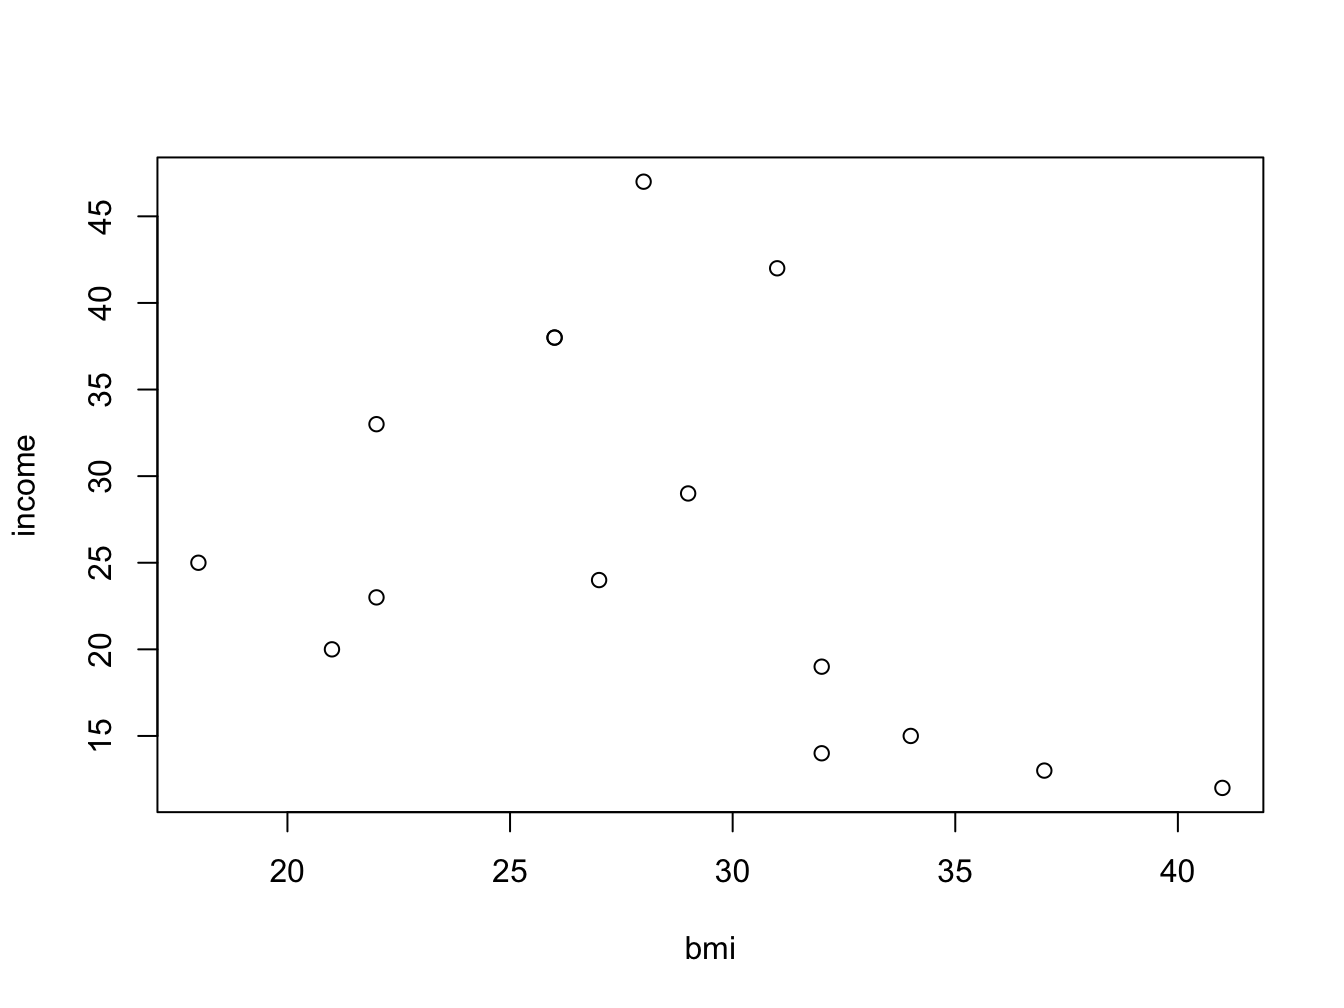
\includegraphics[width=0.7\linewidth]{davur_ebook_files/figure-latex/cut-demo-2-1} \end{center}

But wouldn't it be nice to look at the bmi categories as defined by the WHO? To be able to do this, you need to split the numeric \texttt{bmi} variable into a factor using \texttt{cut()}.

\begin{Shaded}
\begin{Highlighting}[]
\NormalTok{my_data}\OperatorTok{$}\NormalTok{bmi_class <-}\StringTok{ }\KeywordTok{cut}\NormalTok{(bmi,}
    \DataTypeTok{breaks =} \KeywordTok{c}\NormalTok{(}\DecValTok{0}\NormalTok{, }\FloatTok{18.5}\NormalTok{, }\FloatTok{25.0}\NormalTok{, }\FloatTok{30.0}\NormalTok{, }\OtherTok{Inf}\NormalTok{), }
    \DataTypeTok{right =}\NormalTok{ F,}
    \DataTypeTok{labels =} \KeywordTok{c}\NormalTok{(}\StringTok{"underweight"}\NormalTok{, }\StringTok{"normal"}\NormalTok{, }\StringTok{"overweight"}\NormalTok{, }\StringTok{"obese"}\NormalTok{),}
    \DataTypeTok{ordered_result =}\NormalTok{ T)}
\KeywordTok{with}\NormalTok{(my_data, }\KeywordTok{boxplot}\NormalTok{(income }\OperatorTok{~}\StringTok{ }\NormalTok{bmi_class))}
\end{Highlighting}
\end{Shaded}

\begin{center}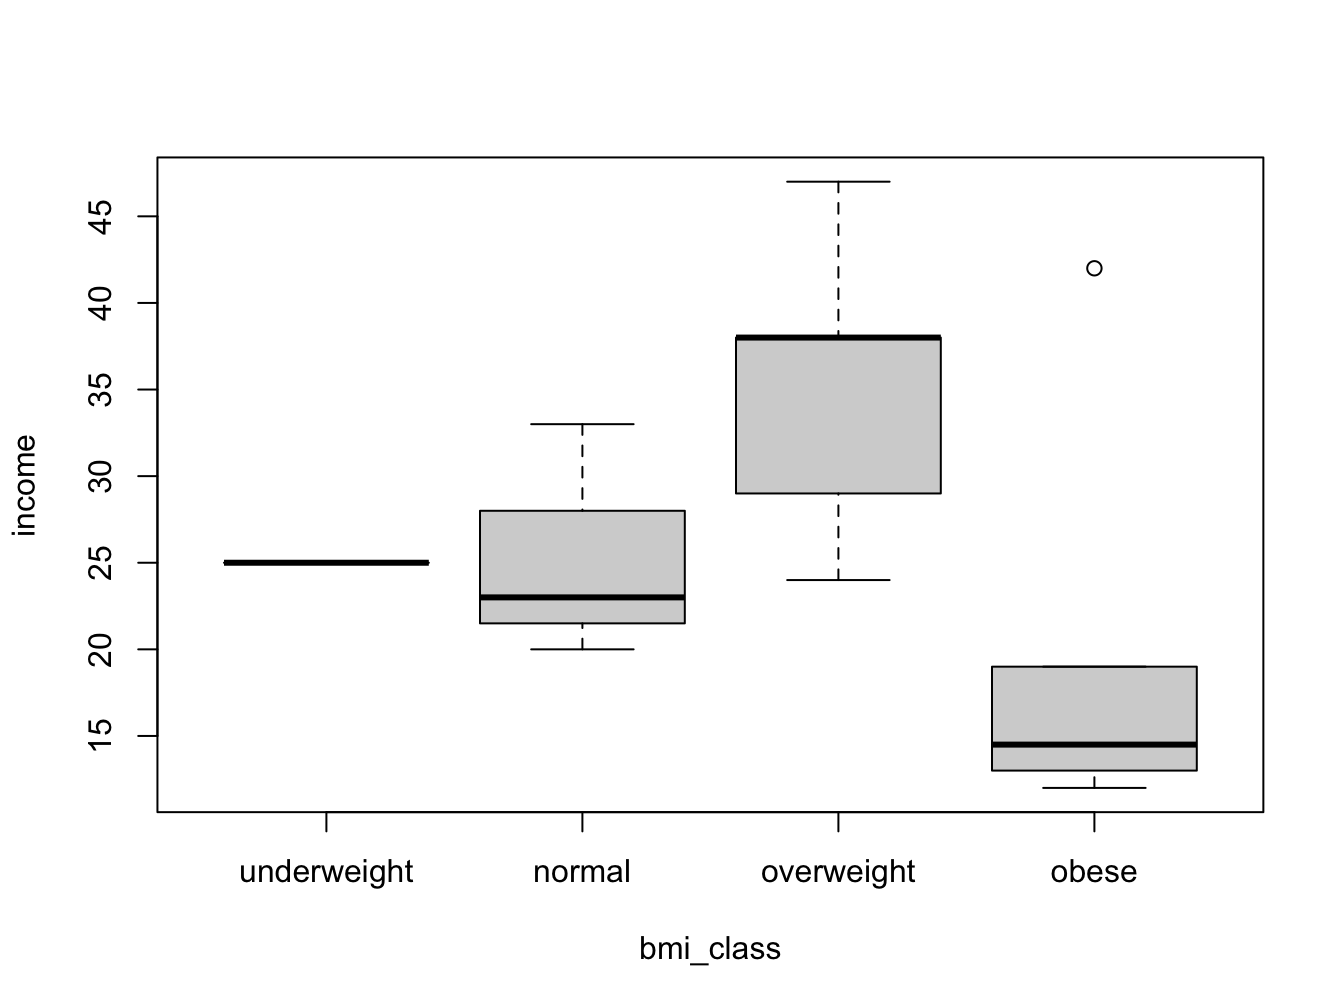
\includegraphics[width=0.7\linewidth]{davur_ebook_files/figure-latex/cut-demo-3-1} \end{center}

The \texttt{breaks\ =} argument specifies the split positions; the \texttt{right\ =\ F} arguments specifies that the interval is \emph{inclusive} on the lower (left) boundary:

\begin{Shaded}
\begin{Highlighting}[]
\NormalTok{x <-}\StringTok{ }\KeywordTok{c}\NormalTok{(}\DecValTok{2}\NormalTok{, }\DecValTok{5}\NormalTok{, }\DecValTok{10}\NormalTok{)}
\KeywordTok{cut}\NormalTok{(x, }\DataTypeTok{breaks =} \KeywordTok{c}\NormalTok{(}\DecValTok{0}\NormalTok{, }\DecValTok{2}\NormalTok{, }\DecValTok{5}\NormalTok{, }\DecValTok{10}\NormalTok{), }\DataTypeTok{right =}\NormalTok{ F)}
\end{Highlighting}
\end{Shaded}

\begin{verbatim}
## [1] [2,5)  [5,10) <NA>  
## Levels: [0,2) [2,5) [5,10)
\end{verbatim}

\begin{Shaded}
\begin{Highlighting}[]
\KeywordTok{cut}\NormalTok{(x, }\DataTypeTok{breaks =} \KeywordTok{c}\NormalTok{(}\DecValTok{0}\NormalTok{, }\DecValTok{2}\NormalTok{, }\DecValTok{5}\NormalTok{, }\DecValTok{10}\NormalTok{), }\DataTypeTok{right =}\NormalTok{ T)}
\end{Highlighting}
\end{Shaded}

\begin{verbatim}
## [1] (0,2]  (2,5]  (5,10]
## Levels: (0,2] (2,5] (5,10]
\end{verbatim}

An interval written as \texttt{(5,10{]}} means it is from -but excluding- 5 to -but including- 10.
Note that in the first example the last value (10) becomes NA because 10 is exclusive in that interval specification.

\hypertarget{file-io-revisited}{%
\section{File I/O revisited}\label{file-io-revisited}}

Whatever the contents of a file, you always need to address (some of) these questions:

\begin{itemize}
\tightlist
\item
  Are there comment lines at the top?
\item
  Is there a header line with column names?
\item
  What is the column separator?
\item
  Are there quotes around character data?
\item
  How are missing values encoded?
\item
  How are numeric values encoded?
\item
  Are there dates (a special challenge)
\item
  What is the type in each column?

  \begin{itemize}
  \tightlist
  \item
    character / numeric / factor / date-time
  \end{itemize}
\end{itemize}

\hypertarget{some-read.table-arguments}{%
\subsubsection*{\texorpdfstring{Some \texttt{read.table()} arguments}{Some read.table() arguments}}\label{some-read.table-arguments}}
\addcontentsline{toc}{subsubsection}{Some \texttt{read.table()} arguments}

\begin{longtable}[]{@{}lll@{}}
\toprule
arg & specifies & example\tabularnewline
\midrule
\endhead
\textbf{sep} & field separator & sep = ``:''\tabularnewline
\textbf{header} & is there a header & header = F\tabularnewline
\textbf{dec} & decimal format & dec = ``,''\tabularnewline
\textbf{comment.char} & comment line start & comment.char = ""\tabularnewline
\textbf{na.strings} & NA value & na.strings = ``-''\tabularnewline
\textbf{as.is} & load as character & as.is = c(1,4)\tabularnewline
\textbf{stringsAsFactors} & load strings as factors & stringsAsFactors = F\tabularnewline
\bottomrule
\end{longtable}

\hypertarget{the-data-reading-workflow}{%
\subsubsection*{The data reading workflow}\label{the-data-reading-workflow}}
\addcontentsline{toc}{subsubsection}{The data reading workflow}

Always apply this sequence of steps and repeat until you are satisfied with the result:

\begin{enumerate}
\def\labelenumi{\arabic{enumi}.}
\tightlist
\item
  \texttt{read.table()} with arguments that seem OK
\item
  Check the result at least with \texttt{str()} and \texttt{head()} and verify that the columns have the correct data type.

  \begin{itemize}
  \tightlist
  \item
    Factors where numeric expected indicate missed ``NA'' values!
  \end{itemize}
\item
  Adjust the read.table parameters
\item
  Rinse and repeat
\end{enumerate}

\hypertarget{writing-data-to-file}{%
\subsubsection*{Writing data to file}\label{writing-data-to-file}}
\addcontentsline{toc}{subsubsection}{Writing data to file}

To write a data frame, matrix or vector to file, use \texttt{write.table(myData,\ file="file.csv")}. Standard is a comma-separated file with both column- and row names, unless otherwise specified:

\begin{itemize}
\tightlist
\item
  \texttt{col.names\ =\ F}
\item
  \texttt{row.names\ =\ F}
\item
  \texttt{sep\ =\ ";"}
\item
  \texttt{sep\ =\ "\textbackslash{}t"\ \#\ tab-separated}
\end{itemize}

\hypertarget{saving-r-objects-to-file}{%
\subsubsection*{Saving R objects to file}\label{saving-r-objects-to-file}}
\addcontentsline{toc}{subsubsection}{Saving R objects to file}

Use the \texttt{save()} function to write R objects to file for later use.
This is especially handy with intermediate results in long-running analysis workflows.

\begin{Shaded}
\begin{Highlighting}[]
\NormalTok{x <-}\StringTok{ }\NormalTok{stats}\OperatorTok{::}\KeywordTok{runif}\NormalTok{(}\DecValTok{20}\NormalTok{)}
\NormalTok{y <-}\StringTok{ }\KeywordTok{list}\NormalTok{(}\DataTypeTok{a =} \DecValTok{1}\NormalTok{, }\DataTypeTok{b =} \OtherTok{TRUE}\NormalTok{, }\DataTypeTok{c =} \StringTok{"oops"}\NormalTok{)}
\KeywordTok{save}\NormalTok{(x, y, }\DataTypeTok{file =} \StringTok{"xy.RData"}\NormalTok{)}
\end{Highlighting}
\end{Shaded}

\hypertarget{writing-a-plot-to-file}{%
\subsubsection*{Writing a plot to file}\label{writing-a-plot-to-file}}
\addcontentsline{toc}{subsubsection}{Writing a plot to file}

Use one of the functions \texttt{png()}, \texttt{jpeg()}, \texttt{tiff()}, or \texttt{bmp()} for these specific file types. They have widely differing properties, especially with respect to file size.\\
Use \texttt{width} and \texttt{height} to specify size. Default unit is pixels. Use other unit: \texttt{units\ =\ "mm"}

\begin{Shaded}
\begin{Highlighting}[]
\KeywordTok{png}\NormalTok{(}\StringTok{"/path/to/your/file.png"}\NormalTok{,}
    \DataTypeTok{width =} \DecValTok{700}\NormalTok{, }\DataTypeTok{height =} \DecValTok{350}\NormalTok{, }\DataTypeTok{units =} \StringTok{"mm"}\NormalTok{)}
\KeywordTok{plot}\NormalTok{(cars)}
\KeywordTok{dev.off}\NormalTok{() }\CommentTok{# don't forget this one!}
\end{Highlighting}
\end{Shaded}

\hypertarget{pattern-matching}{%
\section{Pattern matching}\label{pattern-matching}}

\begin{quote}
Pattern matching is the process of finding, locating, extracting and replacing patterns in character data that usually cannot be literally described.
\end{quote}

For instance, it is easy enough to look for the word ``Chimpanzee'' in a vector containing animal species names:

\begin{Shaded}
\begin{Highlighting}[]
\NormalTok{animals =}\StringTok{ }\KeywordTok{c}\NormalTok{(}\StringTok{"Chimpanzee"}\NormalTok{, }\StringTok{"Cow"}\NormalTok{, }\StringTok{"Camel"}\NormalTok{)}
\NormalTok{animals }\OperatorTok{==}\StringTok{ "Chimpanzee"}
\end{Highlighting}
\end{Shaded}

\begin{verbatim}
## [1]  TRUE FALSE FALSE
\end{verbatim}

but what are you going to do if there are multiple variants of the word you are looking for? This?

\begin{Shaded}
\begin{Highlighting}[]
\NormalTok{animals =}\StringTok{ }\KeywordTok{c}\NormalTok{(}\StringTok{"Chimpanzee"}\NormalTok{, }\StringTok{"Chimp"}\NormalTok{, }\StringTok{"chimpanzee"}\NormalTok{, }\StringTok{"Camel"}\NormalTok{)}
\NormalTok{animals }\OperatorTok{==}\StringTok{ "Chimpanzee"} \OperatorTok{|}\StringTok{ }\NormalTok{animals }\OperatorTok{==}\StringTok{ "Chimp"} \OperatorTok{|}\StringTok{ }\NormalTok{animals }\OperatorTok{==}\StringTok{ "chimpanzee"}
\end{Highlighting}
\end{Shaded}

\begin{verbatim}
## [1]  TRUE  TRUE  TRUE FALSE
\end{verbatim}

The solution here is not using literals, but to describe \textbf{\emph{patterns}}.

Look at the above example. How would you describe a pattern that would correctly identify all Chimpanzee occurrences?

Is you pattern something like this?

\emph{A letter C in upper-or lower case followed by `himp' followed by nothing or `anzee'}

In programming we use \textbf{\emph{regular expressions}} or \textbf{\emph{RegEx}} to describe such a pattern in a formal concise way:

\texttt{{[}Cc{]}himp(anzee)?}

And to apply such a pattern in R, we use one of several functions dedicated for this task. Here is one, \texttt{grepl()}, which returns \texttt{TRUE} if the regex matched the vector element.

\begin{Shaded}
\begin{Highlighting}[]
\KeywordTok{grepl}\NormalTok{(}\StringTok{"[Cc]himp(anzee)?"}\NormalTok{, animals)}
\end{Highlighting}
\end{Shaded}

\begin{verbatim}
## [1]  TRUE  TRUE  TRUE FALSE
\end{verbatim}

\hypertarget{functions-using-regex}{%
\subsubsection*{Functions using regex}\label{functions-using-regex}}
\addcontentsline{toc}{subsubsection}{Functions using regex}

There are several functions dedicated to finding patters in character data. They differ in intent and output. Here is a listing.

\begin{itemize}
\tightlist
\item
  \textbf{finding} Does an element contain a pattern (TRUE/FALSE)? \texttt{grepl(pattern,\ string)}
\item
  \textbf{locating} Which elements contain a pattern (INDEX)? \texttt{grep(pattern,\ string)}
\item
  \textbf{extracting} Get the content of matching elements \texttt{grep(pattern,\ string,\ value\ =\ TRUE)}
\item
  \textbf{replace} Replace the first occurrence of the pattern \texttt{sub(pattern,\ replacement,\ string)}
\item
  \textbf{replace all} Replace all occurrences of the pattern \texttt{gsub(pattern,\ replacement,\ string)}
\end{itemize}

Note that the \texttt{stringr} package from the tidyverse has many user-friendly functions in this field as well. Two of them will be dealt with in the exercises.

\hypertarget{regex-syntax}{%
\subsection{Regex syntax}\label{regex-syntax}}

A regular expression can be build out of any combination of

\begin{itemize}
\tightlist
\item
  \textbf{character sequences} - Literal character sequences such as `chimp'\\
\item
  \textbf{character classes} - A listing of possibilities for a single position.

  \begin{itemize}
  \tightlist
  \item
    Between brackets: \texttt{{[}adgk{]}} means `a' or `d' or `g' or `k'.
  \item
    Use a hyphen to create a series: \texttt{{[}3-9{]}} means digits 3 through 9 and \texttt{{[}a-zA-Z{]}} means all alphabet characters.
  \item
    Negate using \texttt{\^{}}. \texttt{{[}\^{}adgk{]}} means anything \emph{but} a, d, g or k.
  \item
    A special case is the dot \texttt{.}: any character matches.\\
  \item
    Many special character classes exist (digits, whitespaces etc). They are discussed in a later paragraph.
  \end{itemize}
\item
  \textbf{alternatives} - Are defined by the pipe symbol \texttt{\textbar{}}: ``OR''\\
\item
  \textbf{quantifiers} - How many times the preceding block should occur. See next paragraph.\\
\item
  \textbf{anchors} - \texttt{\^{}} means matching at the start of a string. \texttt{\$} means at the end.
\end{itemize}

An excellent cheat sheet from the RStudio website is also included
here

\hypertarget{quantifiers}{%
\subsection{Quantifiers}\label{quantifiers}}

Use quantifiers to specify how many times a character or series of characters should occur.

\begin{itemize}
\tightlist
\item
  \textbf{\texttt{\{n\}}}: exactly \texttt{n} times
\item
  \textbf{\texttt{\{n,\ \}}}: at least \texttt{n} times
\item
  \textbf{\texttt{\{\ ,n\}}}: at most \texttt{n} times
\item
  \textbf{\texttt{\{n,\ m\}}}: at least \texttt{n} and at most \texttt{m} times.
\item
  \textbf{\texttt{*}}: 0 or more times; same as \texttt{\{0,\ \}}
\item
  \textbf{\texttt{+}}: 1 or more times; same as \texttt{\{1,\ \}}
\item
  \textbf{\texttt{?}}: 0 or 1 time; same as \texttt{\{0,\ 1\}}
\end{itemize}

\hypertarget{some-examples}{%
\subsection{Some examples}\label{some-examples}}

\hypertarget{restriction-enzymes}{%
\subsubsection*{Restriction enzymes}\label{restriction-enzymes}}
\addcontentsline{toc}{subsubsection}{Restriction enzymes}

This is the recognition sequence for the \emph{HincII} restriction endonuclease:

\begin{verbatim}
5'-GTYRAC-3'
3'-CARYTG-5'
\end{verbatim}

Before reading on: how would you define a regular expression that is precisely describes this recognition sequence?

Molecular biology sequence ambiguity codes can be found
here

\begin{Shaded}
\begin{Highlighting}[]
\NormalTok{HincII_rs <-}\StringTok{ "GT[CT][AG]AC"}
\NormalTok{sequences <-}\StringTok{ }\KeywordTok{c}\NormalTok{(}\StringTok{"GTCAAC"}\NormalTok{,}
               \StringTok{"GTCGAC"}\NormalTok{,}
               \StringTok{"GTTGAC"}\NormalTok{,}
               \StringTok{"aGTTAACa"}\NormalTok{,}
               \StringTok{"GTGCAC"}\NormalTok{)}
\KeywordTok{grep}\NormalTok{(}\DataTypeTok{pattern =}\NormalTok{ HincII_rs, }\DataTypeTok{x =}\NormalTok{ sequences, }\DataTypeTok{value =} \OtherTok{TRUE}\NormalTok{)}
\end{Highlighting}
\end{Shaded}

\begin{verbatim}
## [1] "GTCAAC"   "GTCGAC"   "GTTGAC"   "aGTTAACa"
\end{verbatim}

\hypertarget{dutch-dates}{%
\subsubsection*{Dutch dates}\label{dutch-dates}}
\addcontentsline{toc}{subsubsection}{Dutch dates}

Here are some Dutch dates, in different accepted formats. The last two are not a correct notation.
Create a RegEx that will determine whether an element contains a Dutch date string.

\begin{Shaded}
\begin{Highlighting}[]
\NormalTok{dates <-}\StringTok{ }\KeywordTok{c}\NormalTok{(}\StringTok{"15/2/2019"}\NormalTok{, }\StringTok{"15-2-2019"}\NormalTok{, }\StringTok{"15-02-2019"}\NormalTok{, }\StringTok{"015/2/20191"}\NormalTok{, }\StringTok{"15/2/20191"}\NormalTok{)}
\NormalTok{dateRegex <-}\StringTok{ "[0-9]\{2\}[/-][0-9]\{1,2\}[/-][0-9]\{4\}"}
\KeywordTok{grep}\NormalTok{(}\DataTypeTok{pattern =}\NormalTok{ dateRegex, }\DataTypeTok{x =}\NormalTok{ dates, }\DataTypeTok{value =} \OtherTok{TRUE}\NormalTok{)}
\end{Highlighting}
\end{Shaded}

\begin{verbatim}
## [1] "15/2/2019"   "15-2-2019"   "15-02-2019"  "015/2/20191" "15/2/20191"
\end{verbatim}

Why were the last two matched?\\
Because the pattern \emph{is there}, albeit embedded in a longer string.\\
We have to \textbf{\emph{anchor}} the pattern to be more specific.

\hypertarget{anchoring}{%
\subsection{Anchoring}\label{anchoring}}

Using anchoring, you can make sure the string is not longer than you explicitly state:

\begin{Shaded}
\begin{Highlighting}[]
\NormalTok{dates <-}\StringTok{ }\KeywordTok{c}\NormalTok{(}\StringTok{"15/2/2019"}\NormalTok{, }\StringTok{"15-2-2019"}\NormalTok{, }\StringTok{"15-02-2019"}\NormalTok{, }\StringTok{"015/2/20191"}\NormalTok{, }\StringTok{"15/2/20191"}\NormalTok{)}
\NormalTok{dateRegex <-}\StringTok{ "^[0-9]\{2\}[/-][0-9]\{1,2\}[/-][0-9]\{4\}$"}
\KeywordTok{grep}\NormalTok{(}\DataTypeTok{pattern =}\NormalTok{ dateRegex, }\DataTypeTok{x =}\NormalTok{ dates, }\DataTypeTok{value =} \OtherTok{TRUE}\NormalTok{)}
\end{Highlighting}
\end{Shaded}

\begin{verbatim}
## [1] "15/2/2019"  "15-2-2019"  "15-02-2019"
\end{verbatim}

Now the date matching is correct.

\hypertarget{metacharacters-special-character-classes}{%
\subsection{Metacharacters: Special character classes}\label{metacharacters-special-character-classes}}

Since patterns such as \texttt{{[}0-9{]}} occur so frequently, they have dedicated character classes such as \texttt{{[}{[}:digit:{]}{]}}. The most important other ones are

\begin{itemize}
\tightlist
\item
  \textbf{digits} \texttt{{[}{[}:digit:{]}{]}} or \texttt{\textbackslash{}\textbackslash{}d}: equivalent to \texttt{{[}0-9{]}}
\item
  \textbf{alphabet characters} \texttt{{[}{[}:alpha:{]}{]}}: equivalent to \texttt{{[}a-zA-Z{]}}
\item
  \textbf{lowercase characters} \texttt{{[}{[}:lower:{]}{]}}: equivalent to \texttt{{[}a-z{]}}
\item
  \textbf{uppercase characters} \texttt{{[}{[}:upper:{]}{]}}: equivalent to \texttt{{[}A-Z{]}}
\item
  \textbf{whitespace characters} \texttt{{[}{[}:space:{]}{]}} or \texttt{\textbackslash{}\textbackslash{}s}: Space, tab, vertical tab, newline, form feed, carriage return
\item
  \textbf{punctuation characters} \texttt{{[}{[}:punct:{]}{]}}: One of !"\#\$\%\&'()*+,-./:;\textless{}=\textgreater{}?@{[}{]}\^{}\_`\{\textbar{}\}\textasciitilde{}
\end{itemize}

(have a look at the cheat sheet for all)

Here is the same example, this time using these predefined character classes

\begin{Shaded}
\begin{Highlighting}[]
\NormalTok{dates <-}\StringTok{ }\KeywordTok{c}\NormalTok{(}\StringTok{"15/2/2019"}\NormalTok{, }\StringTok{"15-2-2019"}\NormalTok{, }\StringTok{"15-02-2019"}\NormalTok{, }\StringTok{"15022019"}\NormalTok{, }\StringTok{"15/2/20191"}\NormalTok{)}
\NormalTok{dateRegex <-}\StringTok{ "[[:digit:]]\{2\}[/-]}\CharTok{\textbackslash{}\textbackslash{}}\StringTok{d\{1,2\}[/-]}\CharTok{\textbackslash{}\textbackslash{}}\StringTok{d\{4\}"}
\KeywordTok{grep}\NormalTok{(}\DataTypeTok{pattern =}\NormalTok{ dateRegex, }\DataTypeTok{x =}\NormalTok{ dates, }\DataTypeTok{value =} \OtherTok{TRUE}\NormalTok{)}
\end{Highlighting}
\end{Shaded}

\begin{verbatim}
## [1] "15/2/2019"  "15-2-2019"  "15-02-2019" "15/2/20191"
\end{verbatim}

\hypertarget{postal-codes}{%
\subsubsection*{Postal codes}\label{postal-codes}}
\addcontentsline{toc}{subsubsection}{Postal codes}

Here are some Dutch zip (postal) codes, in different accepted formats. The last two are not a correct notation.
Can you create a RegEx that will determine whether an element contains a Dutch zip code?

\begin{Shaded}
\begin{Highlighting}[]
\NormalTok{zips <-}\StringTok{ }\KeywordTok{c}\NormalTok{(}\StringTok{"1234 AA"}\NormalTok{, }\StringTok{"2345-BB"}\NormalTok{, }\StringTok{"3456CC"}\NormalTok{, }\StringTok{"4567 dd"}\NormalTok{, }\StringTok{"56789aa"}\NormalTok{, }\StringTok{"6789a_"}\NormalTok{)}
\NormalTok{zips}
\end{Highlighting}
\end{Shaded}

\begin{verbatim}
## [1] "1234 AA" "2345-BB" "3456CC"  "4567 dd" "56789aa" "6789a_"
\end{verbatim}

\hypertarget{prosite-patterns}{%
\subsubsection*{Prosite patterns}\label{prosite-patterns}}
\addcontentsline{toc}{subsubsection}{Prosite patterns}

Prosite is a database of amino acid sequence motifs. One of them is the Histidine Triad profile (PDOC00694).

\begin{verbatim}
[NQAR]-x(4)-[GSAVY]-x-[QFLPA]-x-[LIVMY]-x-[HWYRQ]-  
[LIVMFYST]-H-[LIVMFT]-H-[LIVMF]-[LIVMFPT]-[PSGAWN]
\end{verbatim}

\begin{itemize}
\tightlist
\item
  Write this down as a RegEx
\item
  Was that efficient? Using the \texttt{gsub()} function, can you convert it in a RegEx using code? It may take several iterations. Was that efficient?\\
\item
  Next, use an appropriate function to find if, and where, this pattern is located within the sequences in file \texttt{data/hit\_proteins.txt} (here)
\end{itemize}

Amino Acid codes and Prosite pattern encoding can be found
here

\hypertarget{locating-and-extracting}{%
\subsection{Locating and Extracting}\label{locating-and-extracting}}

This is outside the scope of this first acquaintance. The \texttt{stringr} package from the tidyverse is much better at this than the base R functions. One of the exercises introduces this topic for the eager ones among you.

\hypertarget{scripting}{%
\chapter{Scripting}\label{scripting}}

\hypertarget{introduction}{%
\section{Introduction}\label{introduction}}

So far you have only seen R code used in the console, in code chunks of an RMarkdown document, or maybe in an R script in the form of a scratchpad. The code you have seen consisted of (series of) R statements with one or more function calls.\\
There has been no conditional code, no repeated operations and no extraction of blocks of code into something reusable, a custom function. In short, you have not written any \emph{program} or \emph{script} yet.

This chapter deals with that. It introduces conditional execution and custom functions.

\hypertarget{flow-control}{%
\section{Flow control}\label{flow-control}}

\begin{quote}
Flow control constitutes a series of code elements used to control whether some code blocks are executed or not, and how many times
\end{quote}

These programming concepts and structures are used for flow control:

\begin{itemize}
\tightlist
\item
  Conditional execution: \texttt{if()\{\}\ else\ if()\{\}\ else\{\}}
\item
  Repeated execution: \texttt{for()\ \{\}}
\item
  Repeated conditional execution: \texttt{while()\{\}}
\end{itemize}

For those of you with experience in other programming languages: there is no switch expression. There is a \texttt{switch()} function however, but it is not dealt with in this eBook.

\hypertarget{conditional-execution-with-ifelse}{%
\subsection{\texorpdfstring{Conditional execution with \texttt{if/else}}{Conditional execution with if/else}}\label{conditional-execution-with-ifelse}}

There are several applications for conditionals, with differing language constructs:

\begin{itemize}
\tightlist
\item
  the \texttt{if(COND)\ \{\textless{}TRUE\textgreater{}\}\ else\ \{\textless{}FALSE\textgreater{}\}} code block for controlling program flow
\item
  the \texttt{if\ (COND)\ \textless{}TRUE\textgreater{}\ else\ \textless{}FALSE\textgreater{}} expression as a shorthand for the code block
\item
  the \texttt{ifelse(COND,\ \textless{}TRUE\textgreater{},\ \textless{}FALSE\textgreater{})} function for use on dataframes
\end{itemize}

As you can see there is always a \textbf{\emph{condition}} to be tested. This expression should return a logical value: TRUE or FALSE.

All three are discussed in the following slides.

\hypertarget{the-if-else-code-block}{%
\subsubsection*{\texorpdfstring{The \texttt{if()\ \{\}\ else\ \{\}} code block}{The if() \{\} else \{\} code block}}\label{the-if-else-code-block}}
\addcontentsline{toc}{subsubsection}{The \texttt{if()\ \{\}\ else\ \{\}} code block}

The \texttt{if(COND)\ \{\textless{}TRUE\textgreater{}\}\ else\ \{\textless{}FALSE\textgreater{}\}} code block knows several required and several optional elements.\\
At the minimum there is an \texttt{if(COND)\ \{\}} element where \texttt{COND} is an expression evaluating to a Logical.

\begin{Shaded}
\begin{Highlighting}[]
\NormalTok{age <-}\StringTok{ }\DecValTok{43}
\ControlFlowTok{if}\NormalTok{ (age }\OperatorTok{>=}\StringTok{ }\DecValTok{18}\NormalTok{) \{}
    \KeywordTok{print}\NormalTok{(}\StringTok{"Adult"}\NormalTok{)}
\NormalTok{\}}
\end{Highlighting}
\end{Shaded}

\begin{verbatim}
## [1] "Adult"
\end{verbatim}

\hypertarget{if-shorthand}{%
\subsubsection*{\texorpdfstring{\texttt{if()} shorthand}{if() shorthand}}\label{if-shorthand}}
\addcontentsline{toc}{subsubsection}{\texttt{if()} shorthand}

If there is only one statement within a block you can omit the curly braces:

\begin{Shaded}
\begin{Highlighting}[]
\NormalTok{age <-}\StringTok{ }\DecValTok{43}
\ControlFlowTok{if}\NormalTok{ (age }\OperatorTok{>=}\StringTok{ }\DecValTok{18}\NormalTok{) }\KeywordTok{print}\NormalTok{(}\StringTok{"Adult"}\NormalTok{)}
\end{Highlighting}
\end{Shaded}

\begin{verbatim}
## [1] "Adult"
\end{verbatim}

Remember that the semicolon at the end of a statement is optional in R and is usually omitted.

\hypertarget{if-can-have-an-else}{%
\subsubsection*{\texorpdfstring{\texttt{if()} can have an \texttt{else\ \{\}}}{if() can have an else \{\}}}\label{if-can-have-an-else}}
\addcontentsline{toc}{subsubsection}{\texttt{if()} can have an \texttt{else\ \{\}}}

When there is an alternative course of action when the test evaluates to \texttt{FALSE} you use the \texttt{else\{\}} element of this structure.

\begin{Shaded}
\begin{Highlighting}[]
\NormalTok{age <-}\StringTok{ }\DecValTok{43}
\ControlFlowTok{if}\NormalTok{ (age }\OperatorTok{>=}\StringTok{ }\DecValTok{18}\NormalTok{) \{}
    \KeywordTok{print}\NormalTok{(}\StringTok{"Adult"}\NormalTok{)}
\NormalTok{\} }\ControlFlowTok{else}\NormalTok{ \{}
    \KeywordTok{print}\NormalTok{(}\StringTok{"Junior"}\NormalTok{)}
\NormalTok{\}}
\end{Highlighting}
\end{Shaded}

\begin{verbatim}
## [1] "Adult"
\end{verbatim}

Here the curly braces are required:

\begin{Shaded}
\begin{Highlighting}[]
\NormalTok{age <-}\StringTok{ }\DecValTok{43}
\ControlFlowTok{if}\NormalTok{ (age }\OperatorTok{>=}\StringTok{ }\DecValTok{18}\NormalTok{) }\KeywordTok{print}\NormalTok{(}\StringTok{"Adult"}\NormalTok{)}
\ControlFlowTok{else} \KeywordTok{print}\NormalTok{(}\StringTok{"Junior"}\NormalTok{)}
\end{Highlighting}
\end{Shaded}

\begin{verbatim}
## Error: <text>:3:1: unexpected 'else'
## 2: if (age >= 18) print("Adult")
## 3: else
##    ^
\end{verbatim}

\hypertarget{the-if-can-have-else-if-blocks}{%
\subsubsection*{\texorpdfstring{The \texttt{if()} can have \texttt{else\ if()} blocks}{The if() can have else if() blocks}}\label{the-if-can-have-else-if-blocks}}
\addcontentsline{toc}{subsubsection}{The \texttt{if()} can have \texttt{else\ if()} blocks}

If there are more than two courses of action, you must reside to \texttt{else\ if()} blocks.
Each of them should have its own CONDition to test on.

\begin{Shaded}
\begin{Highlighting}[]
\NormalTok{age <-}\StringTok{ }\DecValTok{43}
\ControlFlowTok{if}\NormalTok{ (age }\OperatorTok{<}\StringTok{ }\DecValTok{18}\NormalTok{) \{}
    \KeywordTok{print}\NormalTok{(}\StringTok{"Minor"}\NormalTok{)}
\NormalTok{\} }\ControlFlowTok{else} \ControlFlowTok{if}\NormalTok{ (age }\OperatorTok{>=}\StringTok{ }\DecValTok{65}\NormalTok{)\{}
    \KeywordTok{print}\NormalTok{(}\StringTok{"Senior"}\NormalTok{)}
\NormalTok{\} }\ControlFlowTok{else} \ControlFlowTok{if}\NormalTok{(age }\OperatorTok{>=}\StringTok{ }\DecValTok{18} \OperatorTok{&&}\StringTok{ }\NormalTok{age }\OperatorTok{<=}\StringTok{ }\DecValTok{30}\NormalTok{)\{}
    \KeywordTok{print}\NormalTok{(}\StringTok{"Young Adult"}\NormalTok{)}
\NormalTok{\} }\ControlFlowTok{else}\NormalTok{ \{}
    \KeywordTok{print}\NormalTok{(}\StringTok{"Adult"}\NormalTok{)}
\NormalTok{\}}
\end{Highlighting}
\end{Shaded}

\begin{verbatim}
## [1] "Adult"
\end{verbatim}

\hypertarget{ifelse-real-life-example}{%
\subsubsection*{if/else real life example}\label{ifelse-real-life-example}}
\addcontentsline{toc}{subsubsection}{if/else real life example}

This code chunk checks if a file exists and only downloads it if it is not present

\begin{Shaded}
\begin{Highlighting}[]
\NormalTok{my_data_file <-}\StringTok{ "/some/file/on/disk"}
\CommentTok{## fetch file}
\ControlFlowTok{if}\NormalTok{ (}\OperatorTok{!}\KeywordTok{file.exists}\NormalTok{(my_data_file)) \{}
    \KeywordTok{print}\NormalTok{(}\KeywordTok{paste}\NormalTok{(}\StringTok{"downloading"}\NormalTok{, my_data_file))}
    \KeywordTok{download.file}\NormalTok{(}\DataTypeTok{url =}\NormalTok{ remote_url, }\DataTypeTok{destfile =}\NormalTok{ my_data_file)}
\NormalTok{\} }\ControlFlowTok{else}\NormalTok{ \{}
    \KeywordTok{print}\NormalTok{(}\KeywordTok{paste}\NormalTok{(}\StringTok{"reading cached copy of"}\NormalTok{, my_data_file))}
\NormalTok{\}}
\end{Highlighting}
\end{Shaded}

\hypertarget{ifelse-shorthand}{%
\subsubsection*{ifelse shorthand}\label{ifelse-shorthand}}
\addcontentsline{toc}{subsubsection}{ifelse shorthand}

There is also a shorthand for \texttt{if()\{\}\ else\{\}}. It is also called a \textbf{\emph{ternary}}.\\
It has the form\\
\texttt{if\ (COND)\ \textless{}EXPRESSION\_FOR\_TRUE\textgreater{}\ else\ \textless{}EXPRESSION\_FOR\_FALSE\textgreater{}}

\begin{Shaded}
\begin{Highlighting}[]
\NormalTok{a <-}\StringTok{ }\DecValTok{3}
\NormalTok{x <-}\StringTok{ }\ControlFlowTok{if}\NormalTok{ (a }\OperatorTok\StringTok{ }\DecValTok{2} \OperatorTok{==}\StringTok{ }\DecValTok{0}\NormalTok{) }\StringTok{"EVEN"} \ControlFlowTok{else} \StringTok{"UNEVEN"}
\NormalTok{x}
\end{Highlighting}
\end{Shaded}

\begin{verbatim}
## [1] "UNEVEN"
\end{verbatim}

\hypertarget{ifelse-on-dataframes-ifelse}{%
\subsubsection*{\texorpdfstring{if/else on dataframes: \texttt{ifelse()}}{if/else on dataframes: ifelse()}}\label{ifelse-on-dataframes-ifelse}}
\addcontentsline{toc}{subsubsection}{if/else on dataframes: \texttt{ifelse()}}

When you want to assign values to a vector based on some condition, you need to use the third form, the \texttt{ifelse()} function.

When you use the regular if/else structures on dataframes you don't get what you want:

\begin{Shaded}
\begin{Highlighting}[]
\CommentTok{# Only first value (row) is evaluated and this value is cycled}
\CommentTok{# The whole column gets value 1}
\NormalTok{airquality}\OperatorTok{$}\NormalTok{foo <-}\StringTok{ }\ControlFlowTok{if}\NormalTok{ (airquality}\OperatorTok{$}\NormalTok{Ozone }\OperatorTok{<}\StringTok{ }\DecValTok{30}\NormalTok{) }\DecValTok{0} \ControlFlowTok{else} \DecValTok{1} 
\end{Highlighting}
\end{Shaded}

\begin{verbatim}
## Warning in if (airquality$Ozone < 30) 0 else 1: the condition has length >
## 1 and only the first element will be used
\end{verbatim}

\begin{Shaded}
\begin{Highlighting}[]
\CommentTok{# This works}
\NormalTok{airquality}\OperatorTok{$}\NormalTok{bar <-}\StringTok{ }\KeywordTok{ifelse}\NormalTok{(airquality}\OperatorTok{$}\NormalTok{Ozone }\OperatorTok{<}\StringTok{ }\DecValTok{30}\NormalTok{, }\DecValTok{0}\NormalTok{, }\DecValTok{1}\NormalTok{)}
\KeywordTok{head}\NormalTok{(airquality)}
\end{Highlighting}
\end{Shaded}

\begin{verbatim}
##   Ozone Solar.R Wind Temp Month Day foo bar
## 1    41     190  7.4   67   May   1   1   1
## 2    36     118  8.0   72   May   2   1   1
## 3    12     149 12.6   74   May   3   1   0
## 4    18     313 11.5   62   May   4   1   0
## 5    NA      NA 14.3   56   May   5   1  NA
## 6    28      NA 14.9   66   May   6   1   0
\end{verbatim}

\hypertarget{iteration-with-for}{%
\subsection{\texorpdfstring{Iteration with \texttt{for()\{\}}}{Iteration with for()\{\}}}\label{iteration-with-for}}

\begin{itemize}
\tightlist
\item
  Iteration with \texttt{for} is used for looping a series of values from a vector.
  \_ You should not use it to iterate columns or rows of a dataframe: the preferred way to do that is with \texttt{apply()} and its relatives (next presentation)
\end{itemize}

\begin{Shaded}
\begin{Highlighting}[]
\ControlFlowTok{for}\NormalTok{ (greeting }\ControlFlowTok{in} \KeywordTok{c}\NormalTok{(}\StringTok{"Hello"}\NormalTok{, }\StringTok{"'Allo"}\NormalTok{, }\StringTok{"Moi"}\NormalTok{)) \{}
    \KeywordTok{print}\NormalTok{(greeting)}
\NormalTok{\}}
\end{Highlighting}
\end{Shaded}

\begin{verbatim}
## [1] "Hello"
## [1] "'Allo"
## [1] "Moi"
\end{verbatim}

Sometimes you need a counter or index when iterating:

\begin{Shaded}
\begin{Highlighting}[]
\NormalTok{greetings <-}\StringTok{ }\KeywordTok{c}\NormalTok{(}\StringTok{"Hello"}\NormalTok{, }\StringTok{"'Allo"}\NormalTok{, }\StringTok{"Moi"}\NormalTok{)}
\ControlFlowTok{for}\NormalTok{ (i }\ControlFlowTok{in} \DecValTok{1} \OperatorTok{:}\StringTok{ }\KeywordTok{length}\NormalTok{(greetings)) \{}
    \KeywordTok{print}\NormalTok{(}\KeywordTok{paste}\NormalTok{(i, greetings[i]))}
\NormalTok{\}}
\end{Highlighting}
\end{Shaded}

\begin{verbatim}
## [1] "1 Hello"
## [1] "2 'Allo"
## [1] "3 Moi"
\end{verbatim}

\hypertarget{conditional-iteration-with-while}{%
\subsection{\texorpdfstring{Conditional iteration with \texttt{while()\{\}}}{Conditional iteration with while()\{\}}}\label{conditional-iteration-with-while}}

This is the last flow control structure. It is used to execute a block \textbf{\emph{as long as a certain condition is met}}. They are not used very much in R.

\begin{Shaded}
\begin{Highlighting}[]
\NormalTok{counter <-}\StringTok{ }\DecValTok{1}
\ControlFlowTok{while}\NormalTok{ (counter }\OperatorTok\StringTok{ }\DecValTok{5} \OperatorTok{!=}\StringTok{ }\DecValTok{0}\NormalTok{) \{}
    \KeywordTok{print}\NormalTok{(counter)}
\NormalTok{    counter =}\StringTok{ }\NormalTok{counter }\OperatorTok{+}\StringTok{ }\DecValTok{1}
\NormalTok{\}}
\end{Highlighting}
\end{Shaded}

\begin{verbatim}
## [1] 1
## [1] 2
## [1] 3
## [1] 4
\end{verbatim}

\hypertarget{creating-functions}{%
\section{Creating functions}\label{creating-functions}}

Here is the definition again.

\begin{quote}
\emph{A function is a piece of functionality that you can execute by typing its name, followed by a pair of parentheses. Within these parentheses, you can pass data for the function to work on. Functions often, but not always, return a value}.
\end{quote}

Thus, functions are named blocks of code with a \textbf{\emph{single well-defined purpose}} which make them reusable.
You have already used many \textbf{\emph{predefined}} or build in functions of R: \texttt{str}, \texttt{max}, \texttt{read.table} etc. If you type the name of a function without parenthesis you get its definition.

\begin{Shaded}
\begin{Highlighting}[]
\NormalTok{sum}
\end{Highlighting}
\end{Shaded}

\begin{verbatim}
## function (..., na.rm = FALSE)  .Primitive("sum")
\end{verbatim}

\hypertarget{anatomy-of-a-function}{%
\subsubsection*{Anatomy of a function}\label{anatomy-of-a-function}}
\addcontentsline{toc}{subsubsection}{Anatomy of a function}

A function

\begin{itemize}
\tightlist
\item
  usually, but not always, has a name. in the next chapter you will see examples of \emph{anonymous} functions that are defined in the location where they are needed.\\
\item
  has a \textbf{\emph{parameter list}} (sometimes of size zero) between parentheses. These parameters constitute the required input variables on which the function will operate.\\
\item
  has a \textbf{\emph{method body}}. This is a block of one or more lines of code in which the actual work is performed.\\
\item
  may have a \textbf{\emph{return value}}. Ther result of a function is usually, but not always returned. The print function, for instance, does not return a value but only outputs to the console. Functions can only retun one single value (vector). If more return values are needed, you need to wrap them in a complex datatype such as a list.\\
\item
  is defined using the \_\textbf{function keyword\_}
\end{itemize}

Here is a function prototype. It shows all characteristics of the above list of properties.

\begin{verbatim}
method_name <- function(arg, arg, ...) {
    <function body>
    return(return_value)
}
\end{verbatim}

\hypertarget{a-first-function}{%
\subsubsection*{A first function}\label{a-first-function}}
\addcontentsline{toc}{subsubsection}{A first function}

Here is a simple function determining whether some number is even

\begin{Shaded}
\begin{Highlighting}[]
\NormalTok{is_even <-}\StringTok{ }\ControlFlowTok{function}\NormalTok{(x) \{}
\NormalTok{    evens <-}\StringTok{ }\NormalTok{x }\OperatorTok\StringTok{ }\DecValTok{2} \OperatorTok{==}\StringTok{ }\DecValTok{0}
    \KeywordTok{return}\NormalTok{(evens) }
\NormalTok{\}}
\KeywordTok{is_even}\NormalTok{(}\DecValTok{1}\OperatorTok{:}\DecValTok{5}\NormalTok{)}
\end{Highlighting}
\end{Shaded}

\begin{verbatim}
## [1] FALSE  TRUE FALSE  TRUE FALSE
\end{verbatim}

Note that \texttt{return()} is a \textbf{\emph{method call}} which is very unlike other programming languages.

The \textbf{\emph{return statement is optional}}.
In R, the last statement of a method body is its \textbf{\emph{implicit return value}}. Therefore, the previous example is equivalent to this:

\begin{Shaded}
\begin{Highlighting}[]
\NormalTok{is_even <-}\StringTok{ }\ControlFlowTok{function}\NormalTok{(x) \{}
\NormalTok{    x }\OperatorTok\StringTok{ }\DecValTok{2} \OperatorTok{==}\StringTok{ }\DecValTok{0}
\NormalTok{\}}
\KeywordTok{is_even}\NormalTok{(}\DecValTok{1}\OperatorTok{:}\DecValTok{5}\NormalTok{)}
\end{Highlighting}
\end{Shaded}

\begin{verbatim}
## [1] FALSE  TRUE FALSE  TRUE FALSE
\end{verbatim}

Being explicit is always allowed when implicit return is possible, but using a \texttt{return()} for forcing return values at other points is required:

\begin{Shaded}
\begin{Highlighting}[]
\NormalTok{my_message <-}\StringTok{ }\ControlFlowTok{function}\NormalTok{(age) \{}
    \ControlFlowTok{if}\NormalTok{ (age }\OperatorTok{<}\StringTok{ }\DecValTok{18}\NormalTok{) }\KeywordTok{return}\NormalTok{(}\StringTok{"have a lemonade!"}\NormalTok{) }\CommentTok{# explicit return}
    \StringTok{"have a beer!"} \CommentTok{# implicit return statement}
\NormalTok{\}}
\KeywordTok{my_message}\NormalTok{(}\DecValTok{20}\NormalTok{)}
\end{Highlighting}
\end{Shaded}

\begin{verbatim}
## [1] "have a beer!"
\end{verbatim}

\hypertarget{default-argument-values}{%
\subsubsection*{Default argument values}\label{default-argument-values}}
\addcontentsline{toc}{subsubsection}{Default argument values}

It is possible to specify \textbf{\emph{default values}} for function arguments. This is a value that is attached to a function parameter when the calling code does not provide one. A default value is specified in the parameter list, using this construct: \texttt{some\_arg\ =\ \textless{}default-value\textgreater{}}. Almost all functions in R have (many) parameters with default values.

You should use default values yourself for function parameters whenever possible. They make using the function so much easier. The following function calculates the exponent (power) of a number. When no \texttt{power\ =} value is provided, it defaults to two.

\begin{Shaded}
\begin{Highlighting}[]
\NormalTok{my_power <-}\StringTok{ }\ControlFlowTok{function}\NormalTok{(x, }\DataTypeTok{power =} \DecValTok{2}\NormalTok{) \{}
\NormalTok{    x }\OperatorTok{^}\StringTok{ }\NormalTok{power}
\NormalTok{\}}
\KeywordTok{my_power}\NormalTok{(}\DecValTok{10}\NormalTok{, }\DecValTok{3}\NormalTok{) }\CommentTok{## custom power}
\end{Highlighting}
\end{Shaded}

\begin{verbatim}
## [1] 1000
\end{verbatim}

\begin{Shaded}
\begin{Highlighting}[]
\KeywordTok{my_power}\NormalTok{(}\DecValTok{10}\NormalTok{) }\CommentTok{## defaults to 2}
\end{Highlighting}
\end{Shaded}

\begin{verbatim}
## [1] 100
\end{verbatim}

\hypertarget{argument-order-when-calling-a-function}{%
\subsubsection*{Argument order when calling a function}\label{argument-order-when-calling-a-function}}
\addcontentsline{toc}{subsubsection}{Argument order when calling a function}

As we have seen many times before, you do not \emph{need} to pass arguments by name. In the above example, the names were not used. When you do not use the names of arguments, the order in which you pass them is important; they must match the order in which they are declared in the function. If you use their names, their order is not important:

\begin{Shaded}
\begin{Highlighting}[]
\KeywordTok{my_power}\NormalTok{(}\DataTypeTok{power =} \DecValTok{4}\NormalTok{, }\DataTypeTok{x =} \DecValTok{2}\NormalTok{)}
\end{Highlighting}
\end{Shaded}

\begin{verbatim}
## [1] 16
\end{verbatim}

To summarize: When calling a function,

\begin{itemize}
\tightlist
\item
  the parameters without default value are mandatory
\item
  the unnamed arguments should come first and should be passed in the order in which they are declared
\item
  passing named arguments may be done in any order
\end{itemize}

\hypertarget{errors-and-warnings}{%
\subsection{Errors and warnings}\label{errors-and-warnings}}

When someting is not right, but not enought to quit execution, use a warning to let the user (or yourself) know that there is something wrong:

\texttt{warning("I\ am\ not\ happy")}

When something is terribly wrong, and you cannot continue, you should stop execution with an error message:

\texttt{stop("I\ can\textquotesingle{}t\ go\ on")}

Here is a small errors demo:

\begin{Shaded}
\begin{Highlighting}[]
\NormalTok{demo_inverse <-}\StringTok{ }\ControlFlowTok{function}\NormalTok{(x) \{}
    \ControlFlowTok{if}\NormalTok{ (}\OperatorTok{!}\KeywordTok{is.numeric}\NormalTok{(x)) \{}
        \KeywordTok{stop}\NormalTok{(}\StringTok{"non-numeric vector"}\NormalTok{)}
\NormalTok{    \}}
    \KeywordTok{return}\NormalTok{(x }\OperatorTok{/}\StringTok{ }\DecValTok{3}\NormalTok{)}
\NormalTok{\}}
\NormalTok{result1 <-}\StringTok{ }\KeywordTok{demo_inverse}\NormalTok{(}\KeywordTok{c}\NormalTok{(}\StringTok{"a"}\NormalTok{, }\StringTok{"b"}\NormalTok{)) }\CommentTok{#result1 not created!}
\end{Highlighting}
\end{Shaded}

\begin{verbatim}
## Error in demo_inverse(c("a", "b")): non-numeric vector
\end{verbatim}

\begin{Shaded}
\begin{Highlighting}[]
\NormalTok{result2 <-}\StringTok{ }\KeywordTok{demo_inverse}\NormalTok{(}\DecValTok{1}\OperatorTok{:}\DecValTok{4}\NormalTok{)}
\end{Highlighting}
\end{Shaded}

\hypertarget{scripting-1}{%
\section{Scripting}\label{scripting-1}}

An R script is a text file with the extension \texttt{.R} that contains R code. When it is loaded, it is immediately evaluated. \textbf{\emph{Functions are loaded/evaluated, but not executed}}. Declared variables are stored in main memory - the Global Environment to be precise.

Here is the contents of a very simple R script called \texttt{source\_demo.R}

\begin{Shaded}
\begin{Highlighting}[]
\NormalTok{x <-}\StringTok{ }\DecValTok{42}
\NormalTok{x }\CommentTok{# echo to console}
\KeywordTok{print}\NormalTok{(}\KeywordTok{paste0}\NormalTok{(}\StringTok{"x = "}\NormalTok{, x)) }\CommentTok{#explicit print}

\CommentTok{# function defined but not called}
\NormalTok{demo_function <-}\StringTok{ }\ControlFlowTok{function}\NormalTok{(message) \{}
    \KeywordTok{print}\NormalTok{(}\KeywordTok{paste}\NormalTok{(}\StringTok{"you said"}\NormalTok{, message))}
\NormalTok{\}}
\end{Highlighting}
\end{Shaded}

You can load this script int your R session by \emph{sourcing} it; just call \texttt{source(path/to/source\_demo.R)}. Alternatively, when you have it open in the RStudio editor, you can click the ``source'' button at the top right of the editor panel. After that, you can use the functions and variables defined within the script:

\begin{Shaded}
\begin{Highlighting}[]
\KeywordTok{source}\NormalTok{(}\StringTok{"data/source_demo.R"}\NormalTok{)}
\end{Highlighting}
\end{Shaded}

\begin{verbatim}
## [1] "x = 42"
\end{verbatim}

\begin{Shaded}
\begin{Highlighting}[]
\NormalTok{x}
\end{Highlighting}
\end{Shaded}

\begin{verbatim}
## [1] 42
\end{verbatim}

\begin{Shaded}
\begin{Highlighting}[]
\KeywordTok{demo_function}\NormalTok{(}\StringTok{"hi!"}\NormalTok{)}
\end{Highlighting}
\end{Shaded}

\begin{verbatim}
## [1] "you said hi!"
\end{verbatim}

\hypertarget{why-scripts}{%
\subsubsection*{Why scripts?}\label{why-scripts}}
\addcontentsline{toc}{subsubsection}{Why scripts?}

\begin{itemize}
\tightlist
\item
  To store pieces of functionality you want to reuse (e.g.~in different RMarkdown documents)
\item
  To store entire workflows outside RMarkdown
\item
  To run R code from the commandline (terminal)
\item
  To call from other scripts and build \textbf{\emph{applications}} or \textbf{\emph{packages}}
\end{itemize}

\hypertarget{dataframe-manipulations-1}{%
\chapter{Dataframe manipulations}\label{dataframe-manipulations-1}}

Dataframes are ubiquitous in R-based data analyses. Many R functions and packages are tailored specifically for DF manipulations - you have already seen \texttt{cbind()}, \texttt{rbind()} and \texttt{subset()}.\\
In this presentation, we'll explore a few new functions and techniques for working with DFs:

\begin{itemize}
\tightlist
\item
  \texttt{apply()}
\item
  \texttt{lapply()}
\item
  \texttt{sapply()}
\item
  \texttt{tapply()}
\item
  \texttt{aggregate()}
\item
  \texttt{split()}
\end{itemize}

\hypertarget{the-apply-family-of-functions}{%
\section{\texorpdfstring{The \texttt{apply()} family of functions}{The apply() family of functions}}\label{the-apply-family-of-functions}}

Looping with \texttt{for} may be tempting, but highly discouraged in R because its inefficient. Ususally one of these functions will do it better:

\begin{itemize}
\tightlist
\item
  \texttt{apply}: Apply a function over the ``margins'' of a dataframe - rows or columns or both
\item
  \texttt{lapply}: Loop over a list and evaluate a function on each element; returns a list of the same length
\item
  \texttt{sapply}: Same as lapply but try to simplify the result
\item
  \texttt{tapply}: Apply a function over subsets of a vector (read: split with a factor)
\end{itemize}

There are more but these are the important ones.

\hypertarget{apply-apply-functions-over-array-margins}{%
\subsection{\texorpdfstring{\texttt{apply()}: Apply Functions Over Array Margins}{apply(): Apply Functions Over Array Margins}}\label{apply-apply-functions-over-array-margins}}

\begin{itemize}
\tightlist
\item
  Suppose you want to know the means of all columns of a dataframe.
\item
  \texttt{apply()} needs to know

  \begin{enumerate}
  \def\labelenumi{\arabic{enumi}.}
  \tightlist
  \item
    what DF to apply to (\texttt{X})
  \item
    over which margin(s) - columns and/or rows (\texttt{MARGIN})
  \item
    what function to apply (\texttt{FUN})
  \end{enumerate}
\end{itemize}

\begin{Shaded}
\begin{Highlighting}[]
\KeywordTok{apply}\NormalTok{(}\DataTypeTok{X =}\NormalTok{ cars, }\DataTypeTok{MARGIN =} \DecValTok{2}\NormalTok{, }\DataTypeTok{FUN =}\NormalTok{ mean) }\CommentTok{# apply over columns}
\end{Highlighting}
\end{Shaded}

\begin{verbatim}
## speed  dist 
## 15.40 42.98
\end{verbatim}

Here, a function is applied to both columns and rows

\begin{Shaded}
\begin{Highlighting}[]
\NormalTok{df <-}\StringTok{ }\KeywordTok{data.frame}\NormalTok{(}\DataTypeTok{x =} \DecValTok{1}\OperatorTok{:}\DecValTok{5}\NormalTok{, }\DataTypeTok{y =} \DecValTok{6}\OperatorTok{:}\DecValTok{10}\NormalTok{)}
\NormalTok{minus_one_squared <-}\StringTok{ }\ControlFlowTok{function}\NormalTok{(x) (x}\DecValTok{-1}\NormalTok{)}\OperatorTok{^}\DecValTok{2}
\KeywordTok{apply}\NormalTok{(}\DataTypeTok{X =}\NormalTok{ df, }\DataTypeTok{MARGIN =} \KeywordTok{c}\NormalTok{(}\DecValTok{1}\NormalTok{,}\DecValTok{2}\NormalTok{), }\DataTypeTok{FUN =}\NormalTok{ minus_one_squared)}
\end{Highlighting}
\end{Shaded}

\begin{verbatim}
##       x  y
## [1,]  0 25
## [2,]  1 36
## [3,]  4 49
## [4,]  9 64
## [5,] 16 81
\end{verbatim}

(Ok, that was a bit lame: \texttt{minus\_one\_squared(df)} does the same)

The Body Mass Index, or BMI, is calculated as \((weight / height ^ 2) * 703\) where weight is in pounds and height in inches. Here it is calculated for the build in dataset \texttt{women}.

\begin{Shaded}
\begin{Highlighting}[]
\KeywordTok{head}\NormalTok{(women, }\DataTypeTok{n=}\DecValTok{3}\NormalTok{)}
\end{Highlighting}
\end{Shaded}

\begin{verbatim}
##   height weight
## 1     58    115
## 2     59    117
## 3     60    120
\end{verbatim}

\begin{Shaded}
\begin{Highlighting}[]
\NormalTok{women}\OperatorTok{$}\NormalTok{bmi <-}\StringTok{ }\KeywordTok{apply}\NormalTok{(}\DataTypeTok{X =}\NormalTok{ women, }
                   \DataTypeTok{MARGIN =} \DecValTok{1}\NormalTok{, }
                   \DataTypeTok{FUN =} \ControlFlowTok{function}\NormalTok{(x) (x[}\DecValTok{2}\NormalTok{] }\OperatorTok{/}\StringTok{ }\NormalTok{x[}\DecValTok{1}\NormalTok{]}\OperatorTok{^}\DecValTok{2}\NormalTok{) }\OperatorTok{*}\StringTok{ }\DecValTok{703}\NormalTok{)}
\KeywordTok{head}\NormalTok{(women, }\DataTypeTok{n=}\DecValTok{4}\NormalTok{)}
\end{Highlighting}
\end{Shaded}

\begin{verbatim}
##   height weight   bmi
## 1     58    115 24.03
## 2     59    117 23.63
## 3     60    120 23.43
## 4     61    123 23.24
\end{verbatim}

\hypertarget{pass-arguments-to-the-applied-function}{%
\subsubsection*{Pass arguments to the applied function}\label{pass-arguments-to-the-applied-function}}
\addcontentsline{toc}{subsubsection}{Pass arguments to the applied function}

Sometimes the applied function needs to have other arguments passed besides the row or column. The \texttt{...} argument to \texttt{apply()} makes this possible (type \texttt{?apply} to see more info)

\begin{Shaded}
\begin{Highlighting}[]
\CommentTok{# function sums and powers up}
\NormalTok{spwr <-}\StringTok{ }\ControlFlowTok{function}\NormalTok{(x, }\DataTypeTok{p =} \DecValTok{2}\NormalTok{) \{}\KeywordTok{sum}\NormalTok{(x)}\OperatorTok{^}\NormalTok{p\}}
\CommentTok{# a simple dataframe}
\NormalTok{df <-}\StringTok{ }\KeywordTok{data.frame}\NormalTok{(}\DataTypeTok{a =} \DecValTok{1}\OperatorTok{:}\DecValTok{5}\NormalTok{, }\DataTypeTok{b =} \DecValTok{6}\OperatorTok{:}\DecValTok{10}\NormalTok{)}
\NormalTok{df}
\end{Highlighting}
\end{Shaded}

\begin{verbatim}
##   a  b
## 1 1  6
## 2 2  7
## 3 3  8
## 4 4  9
## 5 5 10
\end{verbatim}

\begin{Shaded}
\begin{Highlighting}[]
\CommentTok{# spwr will use the default value for p (p = 2)}
\KeywordTok{apply}\NormalTok{(}\DataTypeTok{X =}\NormalTok{ df, }\DataTypeTok{MARGIN =} \DecValTok{1}\NormalTok{, }\DataTypeTok{FUN =}\NormalTok{ spwr) }
\end{Highlighting}
\end{Shaded}

\begin{verbatim}
## [1]  49  81 121 169 225
\end{verbatim}

\begin{Shaded}
\begin{Highlighting}[]
\CommentTok{# pass power p = 3 to function spwr (argument names omitted)}
\KeywordTok{apply}\NormalTok{(df, }\DecValTok{1}\NormalTok{, spwr, }\DataTypeTok{p =} \DecValTok{3}\NormalTok{) }
\end{Highlighting}
\end{Shaded}

\begin{verbatim}
## [1]  343  729 1331 2197 3375
\end{verbatim}

Note: The \texttt{...} argument works for all \texttt{..apply..} functions.

\hypertarget{lapply-apply-a-function-over-a-list-or-vector}{%
\subsection{\texorpdfstring{\texttt{lapply()}: Apply a Function over a List or Vector}{lapply(): Apply a Function over a List or Vector}}\label{lapply-apply-a-function-over-a-list-or-vector}}

Function \texttt{lapply()} applies a function to all elements of a list and returns a list with the same length, each element the result of applying the function

\begin{Shaded}
\begin{Highlighting}[]
\NormalTok{myNumbers =}\StringTok{ }\KeywordTok{list}\NormalTok{(}
    \DataTypeTok{one =} \KeywordTok{c}\NormalTok{(}\DecValTok{1}\NormalTok{, }\DecValTok{3}\NormalTok{, }\DecValTok{4}\NormalTok{), }
    \DataTypeTok{two =} \KeywordTok{c}\NormalTok{(}\DecValTok{3}\NormalTok{, }\DecValTok{2}\NormalTok{, }\DecValTok{6}\NormalTok{, }\DecValTok{1}\NormalTok{), }
    \DataTypeTok{three =} \KeywordTok{c}\NormalTok{(}\DecValTok{5}\NormalTok{, }\DecValTok{7}\NormalTok{, }\DecValTok{6}\NormalTok{, }\DecValTok{8}\NormalTok{, }\DecValTok{9}\NormalTok{))}
\KeywordTok{lapply}\NormalTok{(}\DataTypeTok{X =}\NormalTok{ myNumbers, }\DataTypeTok{FUN =}\NormalTok{ mean)}
\end{Highlighting}
\end{Shaded}

\begin{verbatim}
## $one
## [1] 2.667
## 
## $two
## [1] 3
## 
## $three
## [1] 7
\end{verbatim}

Here is the same list, but now with \texttt{sqrt()} applied. Notice how the nature of the applied function influences the result.

\begin{Shaded}
\begin{Highlighting}[]
\KeywordTok{lapply}\NormalTok{(}\DataTypeTok{X =}\NormalTok{ myNumbers, }\DataTypeTok{FUN =}\NormalTok{ sqrt)}
\end{Highlighting}
\end{Shaded}

\begin{verbatim}
## $one
## [1] 1.000 1.732 2.000
## 
## $two
## [1] 1.732 1.414 2.449 1.000
## 
## $three
## [1] 2.236 2.646 2.449 2.828 3.000
\end{verbatim}

\hypertarget{sapply-apply-a-function-over-a-list-or-vector-and-simplify}{%
\subsection{\texorpdfstring{\texttt{sapply()}: Apply a Function over a List or Vector and Simplify}{sapply(): Apply a Function over a List or Vector and Simplify}}\label{sapply-apply-a-function-over-a-list-or-vector-and-simplify}}

When using the same example as above, but with \texttt{sapply}, you get a vector returned. Note that the resulting vector is a named vector, a convenient feature of \texttt{sapply}

\begin{Shaded}
\begin{Highlighting}[]
\NormalTok{myNumbers =}\StringTok{ }\KeywordTok{list}\NormalTok{(}
    \DataTypeTok{one =} \KeywordTok{c}\NormalTok{(}\DecValTok{1}\NormalTok{, }\DecValTok{3}\NormalTok{, }\DecValTok{4}\NormalTok{),}
    \DataTypeTok{two =} \KeywordTok{c}\NormalTok{(}\DecValTok{3}\NormalTok{, }\DecValTok{2}\NormalTok{, }\DecValTok{6}\NormalTok{, }\DecValTok{1}\NormalTok{),}
    \DataTypeTok{three =} \KeywordTok{c}\NormalTok{(}\DecValTok{5}\NormalTok{, }\DecValTok{7}\NormalTok{, }\DecValTok{6}\NormalTok{, }\DecValTok{8}\NormalTok{, }\DecValTok{9}\NormalTok{))}
\KeywordTok{sapply}\NormalTok{(}\DataTypeTok{X =}\NormalTok{ myNumbers, }\DataTypeTok{FUN =}\NormalTok{ mean)}
\end{Highlighting}
\end{Shaded}

\begin{verbatim}
##   one   two three 
## 2.667 3.000 7.000
\end{verbatim}

When the result can not be simplified, you get the same list as with \texttt{lapply()}:

\begin{Shaded}
\begin{Highlighting}[]
\KeywordTok{sapply}\NormalTok{(}\DataTypeTok{X =}\NormalTok{ myNumbers, }\DataTypeTok{FUN =}\NormalTok{ sqrt)}
\end{Highlighting}
\end{Shaded}

\begin{verbatim}
## $one
## [1] 1.000 1.732 2.000
## 
## $two
## [1] 1.732 1.414 2.449 1.000
## 
## $three
## [1] 2.236 2.646 2.449 2.828 3.000
\end{verbatim}

\hypertarget{wasnt-a-dataframe-also-a-list}{%
\subsubsection{wasn't a dataframe also a list?}\label{wasnt-a-dataframe-also-a-list}}

Yes! It is also list(ish). Both \texttt{lapply()} and \texttt{sapply()} work just fine on dataframes:

\begin{Shaded}
\begin{Highlighting}[]
\KeywordTok{lapply}\NormalTok{(}\DataTypeTok{X =}\NormalTok{ cars, }\DataTypeTok{FUN =}\NormalTok{ mean)}
\end{Highlighting}
\end{Shaded}

\begin{verbatim}
## $speed
## [1] 15.4
## 
## $dist
## [1] 42.98
\end{verbatim}

\begin{Shaded}
\begin{Highlighting}[]
\KeywordTok{sapply}\NormalTok{(}\DataTypeTok{X =}\NormalTok{ cars, }\DataTypeTok{FUN =}\NormalTok{ mean) }
\end{Highlighting}
\end{Shaded}

\begin{verbatim}
## speed  dist 
## 15.40 42.98
\end{verbatim}

By the way, sapply and lapply also work with vectors.

\hypertarget{tapply-apply-a-function-over-a-ragged-array}{%
\subsection{\texorpdfstring{\texttt{tapply()}: Apply a Function Over a Ragged Array}{tapply(): Apply a Function Over a Ragged Array}}\label{tapply-apply-a-function-over-a-ragged-array}}

What \texttt{tapply()} does is apply a function over subsets of a vector; it splits a vector into groups according to the levels in a second vector and applies the given function to each group.

\begin{Shaded}
\begin{Highlighting}[]
\KeywordTok{tapply}\NormalTok{(}\DataTypeTok{X =}\NormalTok{ chickwts}\OperatorTok{$}\NormalTok{weight, }\DataTypeTok{INDEX =}\NormalTok{ chickwts}\OperatorTok{$}\NormalTok{feed, }\DataTypeTok{FUN =}\NormalTok{ sd)}
\end{Highlighting}
\end{Shaded}

\begin{verbatim}
##    casein horsebean   linseed  meatmeal   soybean sunflower 
##     64.43     38.63     52.24     64.90     54.13     48.84
\end{verbatim}

\hypertarget{split-divide-into-groups-and-reassemble}{%
\subsection{\texorpdfstring{\texttt{split()}: Divide into Groups and Reassemble}{split(): Divide into Groups and Reassemble}}\label{split-divide-into-groups-and-reassemble}}

This is similar to \texttt{tapply()} in the sense that is uses a factor to split its first argument. But where \texttt{tapply()} splits a vector, \texttt{split()} splits a dataframe - into \emph{list of dataframes}.
You use \texttt{split()} when a dataframe needs to be divided depending on the value of some grouping variable.\\
Here we have the response of Treated (T) and Untreated (UT) subjects

\begin{Shaded}
\begin{Highlighting}[]
\NormalTok{myData <-}\StringTok{ }\KeywordTok{data.frame}\NormalTok{(}
    \DataTypeTok{response =} \KeywordTok{c}\NormalTok{(}\DecValTok{5}\NormalTok{, }\DecValTok{8}\NormalTok{, }\DecValTok{4}\NormalTok{, }\DecValTok{5}\NormalTok{, }\DecValTok{9}\NormalTok{, }\DecValTok{3}\NormalTok{, }\DecValTok{6}\NormalTok{, }\DecValTok{7}\NormalTok{, }\DecValTok{3}\NormalTok{, }\DecValTok{6}\NormalTok{, }\DecValTok{5}\NormalTok{, }\DecValTok{2}\NormalTok{),}
    \DataTypeTok{treatment =} \KeywordTok{factor}\NormalTok{(}
        \KeywordTok{c}\NormalTok{(}\StringTok{"UT"}\NormalTok{, }\StringTok{"T"}\NormalTok{, }\StringTok{"UT"}\NormalTok{, }\StringTok{"UT"}\NormalTok{, }\StringTok{"T"}\NormalTok{, }\StringTok{"UT"}\NormalTok{, }\StringTok{"T"}\NormalTok{, }\StringTok{"T"}\NormalTok{, }\StringTok{"UT"}\NormalTok{, }\StringTok{"T"}\NormalTok{, }\StringTok{"T"}\NormalTok{, }\StringTok{"UT"}\NormalTok{)))}
\NormalTok{splData <-}\StringTok{ }\KeywordTok{split}\NormalTok{(}\DataTypeTok{x =}\NormalTok{ myData, }\DataTypeTok{f =}\NormalTok{ myData}\OperatorTok{$}\NormalTok{treatment)}
\KeywordTok{str}\NormalTok{(splData)}
\end{Highlighting}
\end{Shaded}

\begin{verbatim}
## List of 2
##  $ T :'data.frame':  6 obs. of  2 variables:
##   ..$ response : num [1:6] 8 9 6 7 6 5
##   ..$ treatment: Factor w/ 2 levels "T","UT": 1 1 1 1 1 1
##  $ UT:'data.frame':  6 obs. of  2 variables:
##   ..$ response : num [1:6] 5 4 5 3 3 2
##   ..$ treatment: Factor w/ 2 levels "T","UT": 2 2 2 2 2 2
\end{verbatim}

\begin{Shaded}
\begin{Highlighting}[]
\KeywordTok{boxplot}\NormalTok{(splData}\OperatorTok{$}\NormalTok{T}\OperatorTok{$}\NormalTok{response, splData}\OperatorTok{$}\NormalTok{UT}\OperatorTok{$}\NormalTok{response, }
        \DataTypeTok{names =} \KeywordTok{c}\NormalTok{(}\StringTok{"Treated"}\NormalTok{, }\StringTok{"Untreated"}\NormalTok{))}
\end{Highlighting}
\end{Shaded}

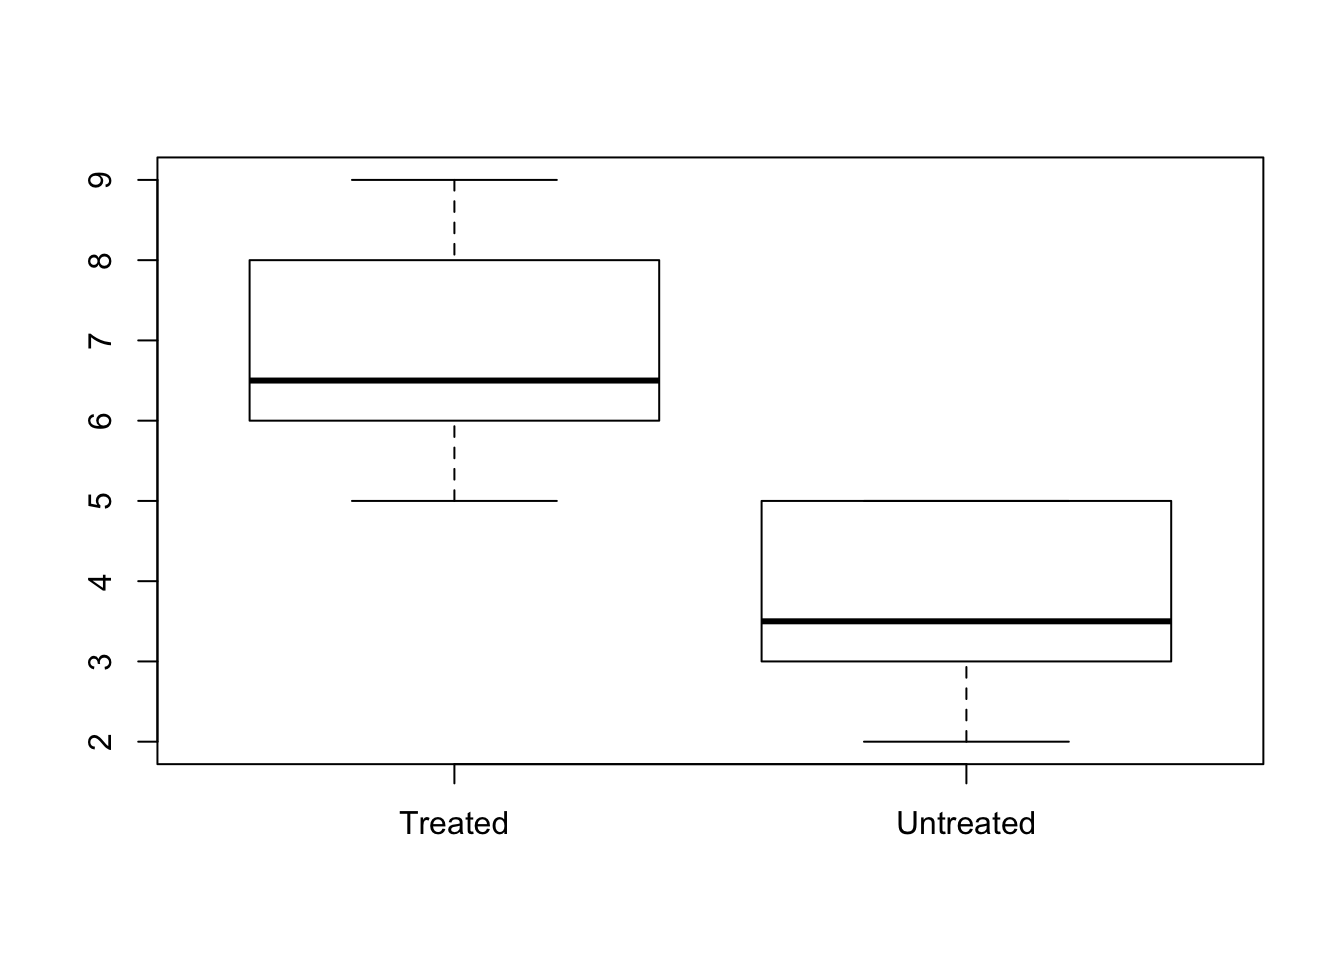
\includegraphics{davur_ebook_files/figure-latex/split_demo1-1.pdf}

Note that this trivial example could also have been done with \texttt{boxplot(myData\$response\ \textasciitilde{}\ myData\$treatment)}.

Here you can see that \texttt{split()} also works with vectors.

\begin{Shaded}
\begin{Highlighting}[]
\KeywordTok{split}\NormalTok{(}\DataTypeTok{x =} \KeywordTok{rnorm}\NormalTok{(}\DecValTok{10}\NormalTok{), }\DataTypeTok{f =} \KeywordTok{rep}\NormalTok{(}\KeywordTok{c}\NormalTok{(}\StringTok{"sick"}\NormalTok{, }\StringTok{"healthy"}\NormalTok{), }\DataTypeTok{each=}\DecValTok{5}\NormalTok{))}
\end{Highlighting}
\end{Shaded}

\begin{verbatim}
## $healthy
## [1] -0.35028  1.37414 -0.29972  0.09764  0.38119
## 
## $sick
## [1]  1.1886  1.0599  1.3368 -0.3672 -0.3043
\end{verbatim}

\hypertarget{aggregate-compute-summary-statistics-of-data-subsets}{%
\subsection{\texorpdfstring{\texttt{aggregate()}: Compute Summary Statistics of Data Subsets}{aggregate(): Compute Summary Statistics of Data Subsets}}\label{aggregate-compute-summary-statistics-of-data-subsets}}

Splits the data into subsets, computes summary statistics for each, and returns the result in a convenient form.

\begin{Shaded}
\begin{Highlighting}[]
\KeywordTok{aggregate}\NormalTok{(}\DataTypeTok{formula =}\NormalTok{ Temp }\OperatorTok{~}\StringTok{ }\NormalTok{Month, }\DataTypeTok{data =}\NormalTok{ airquality, }\DataTypeTok{FUN =}\NormalTok{ mean)}
\end{Highlighting}
\end{Shaded}

\begin{verbatim}
##       Month  Temp
## 1       May 65.55
## 2      June 79.10
## 3      July 83.90
## 4    August 83.97
## 5 September 76.90
\end{verbatim}

Aggregate has two usage techniques:

\begin{itemize}
\item
  with a formula:\\
  \textbf{\texttt{aggregate(formula,\ data,\ FUN,\ ...)}}
\item
  with a list:\\
  \textbf{\texttt{aggregate(x,\ by,\ FUN,\ ...)}}
\end{itemize}

I really like \texttt{aggregate()}, especially the first form. That is, until I got to know the \texttt{dplyr} package.

Both forms of \texttt{aggregate()} will be demonstrated

\hypertarget{aggregate-with-formula}{%
\subsubsection*{Aggregate with formula}\label{aggregate-with-formula}}
\addcontentsline{toc}{subsubsection}{Aggregate with formula}

The left part of the formula accepts one, several or all columns as dependent variables.

\begin{Shaded}
\begin{Highlighting}[]
\CommentTok{##two dependents}
\KeywordTok{aggregate}\NormalTok{(}\KeywordTok{cbind}\NormalTok{(Temp, Ozone) }\OperatorTok{~}\StringTok{ }\NormalTok{Month, }\DataTypeTok{data =}\NormalTok{ airquality, }\DataTypeTok{FUN =}\NormalTok{ mean)}
\end{Highlighting}
\end{Shaded}

\begin{verbatim}
##       Month  Temp Ozone
## 1       May 66.73 23.62
## 2      June 78.22 29.44
## 3      July 83.88 59.12
## 4    August 83.96 59.96
## 5 September 76.90 31.45
\end{verbatim}

\begin{Shaded}
\begin{Highlighting}[]
\CommentTok{##all}
\KeywordTok{aggregate}\NormalTok{(. }\OperatorTok{~}\StringTok{ }\NormalTok{Month, }\DataTypeTok{data =}\NormalTok{ airquality, }\DataTypeTok{FUN =}\NormalTok{ mean)}
\end{Highlighting}
\end{Shaded}

\begin{verbatim}
##       Month Ozone Solar.R   Wind  Temp   Day foo    bar
## 1       May 24.12   182.0 11.504 66.46 16.08   1 0.3333
## 2      June 29.44   184.2 12.178 78.22 14.33   1 0.3333
## 3      July 59.12   216.4  8.523 83.88 16.23   1 0.8077
## 4    August 60.00   173.1  8.861 83.70 17.17   1 0.6957
## 5 September 31.45   168.2 10.076 76.90 15.10   1 0.3448
\end{verbatim}

The right part can also accept multiple independent variables

\begin{Shaded}
\begin{Highlighting}[]
\NormalTok{airquality}\OperatorTok{$}\NormalTok{Temp_factor <-}\StringTok{ }\KeywordTok{cut}\NormalTok{(airquality}\OperatorTok{$}\NormalTok{Temp, }\DataTypeTok{breaks =} \DecValTok{2}\NormalTok{, }\DataTypeTok{labels =} \KeywordTok{c}\NormalTok{(}\StringTok{"low"}\NormalTok{, }\StringTok{"high"}\NormalTok{))}
\KeywordTok{aggregate}\NormalTok{(Ozone }\OperatorTok{~}\StringTok{ }\NormalTok{Month }\OperatorTok{+}\StringTok{ }\NormalTok{Temp_factor, }\DataTypeTok{data =}\NormalTok{ airquality, }\DataTypeTok{FUN =}\NormalTok{ mean)}
\end{Highlighting}
\end{Shaded}

\begin{verbatim}
##        Month Temp_factor Ozone
## 1        May         low 18.92
## 2       June         low 20.50
## 3       July         low 13.00
## 4     August         low 16.00
## 5  September         low 17.62
## 6        May        high 80.00
## 7       June        high 36.60
## 8       July        high 62.96
## 9     August        high 63.62
## 10 September        high 48.46
\end{verbatim}

\hypertarget{the-by-list...-form}{%
\subsubsection*{\texorpdfstring{The \texttt{by\ =\ list(...)} form}{The by = list(...) form}}\label{the-by-list...-form}}
\addcontentsline{toc}{subsubsection}{The \texttt{by\ =\ list(...)} form}

This is the other form of aggregate. It is more elaborate in my opinion because you need te spell out all vectors you want to work on.

\begin{Shaded}
\begin{Highlighting}[]
\KeywordTok{aggregate}\NormalTok{(}\DataTypeTok{x =}\NormalTok{ chickwts}\OperatorTok{$}\NormalTok{weight, }\DataTypeTok{by =} \KeywordTok{list}\NormalTok{(}\DataTypeTok{feed =}\NormalTok{ chickwts}\OperatorTok{$}\NormalTok{feed), }\DataTypeTok{FUN =}\NormalTok{ mean)}
\end{Highlighting}
\end{Shaded}

\begin{verbatim}
##        feed     x
## 1    casein 323.6
## 2 horsebean 160.2
## 3   linseed 218.8
## 4  meatmeal 276.9
## 5   soybean 246.4
## 6 sunflower 328.9
\end{verbatim}

Here is another example:

\begin{Shaded}
\begin{Highlighting}[]
\KeywordTok{aggregate}\NormalTok{(}\DataTypeTok{x =}\NormalTok{ airquality}\OperatorTok{$}\NormalTok{Wind, }
          \DataTypeTok{by =} \KeywordTok{list}\NormalTok{(}\DataTypeTok{month =}\NormalTok{ airquality}\OperatorTok{$}\NormalTok{Month, }\DataTypeTok{temperature =}\NormalTok{ airquality}\OperatorTok{$}\NormalTok{Temp_factor), }
          \DataTypeTok{FUN =}\NormalTok{ mean)}
\end{Highlighting}
\end{Shaded}

\begin{verbatim}
##        month temperature      x
## 1        May         low 11.714
## 2       June         low  9.855
## 3       July         low 10.600
## 4     August         low 11.433
## 5  September         low 11.394
## 6        May        high 10.300
## 7       June        high 10.505
## 8       July        high  8.828
## 9     August        high  8.511
## 10 September        high  8.793
\end{verbatim}

But it is better to wrap it in \texttt{with()}:

\begin{Shaded}
\begin{Highlighting}[]
\KeywordTok{with}\NormalTok{(airquality, }\KeywordTok{aggregate}\NormalTok{(}\DataTypeTok{x =}\NormalTok{ Wind, }
                           \DataTypeTok{by =} \KeywordTok{list}\NormalTok{(}\DataTypeTok{month =}\NormalTok{ Month, }\DataTypeTok{temperature =}\NormalTok{ Temp_factor), }
                           \DataTypeTok{FUN =}\NormalTok{ mean))}
\end{Highlighting}
\end{Shaded}

\hypertarget{many-roads-lead-to-rome}{%
\subsection{Many roads lead to Rome}\label{many-roads-lead-to-rome}}

The next series of examples are all essentially the same. The message is: there is more than one way to do it!

\begin{Shaded}
\begin{Highlighting}[]
\KeywordTok{aggregate}\NormalTok{(weight }\OperatorTok{~}\StringTok{ }\NormalTok{feed, }\DataTypeTok{data =}\NormalTok{ chickwts, }\DataTypeTok{FUN =}\NormalTok{ mean)}
\end{Highlighting}
\end{Shaded}

\begin{verbatim}
##        feed weight
## 1    casein  323.6
## 2 horsebean  160.2
## 3   linseed  218.8
## 4  meatmeal  276.9
## 5   soybean  246.4
## 6 sunflower  328.9
\end{verbatim}

same as

\begin{Shaded}
\begin{Highlighting}[]
\KeywordTok{head}\NormalTok{(}\KeywordTok{aggregate}\NormalTok{(}\DataTypeTok{x =}\NormalTok{ chickwts}\OperatorTok{$}\NormalTok{weight, }\DataTypeTok{by =} \KeywordTok{list}\NormalTok{(}\DataTypeTok{feed =}\NormalTok{ chickwts}\OperatorTok{$}\NormalTok{feed), }\DataTypeTok{FUN =}\NormalTok{ mean), }\DataTypeTok{n=}\DecValTok{3}\NormalTok{)}
\end{Highlighting}
\end{Shaded}

\begin{verbatim}
##        feed     x
## 1    casein 323.6
## 2 horsebean 160.2
## 3   linseed 218.8
\end{verbatim}

same as

\begin{Shaded}
\begin{Highlighting}[]
\KeywordTok{tapply}\NormalTok{(chickwts}\OperatorTok{$}\NormalTok{weight, chickwts}\OperatorTok{$}\NormalTok{feed, mean)}
\end{Highlighting}
\end{Shaded}

\begin{verbatim}
##    casein horsebean   linseed  meatmeal   soybean sunflower 
##     323.6     160.2     218.8     276.9     246.4     328.9
\end{verbatim}

\begin{Shaded}
\begin{Highlighting}[]
\KeywordTok{with}\NormalTok{(chickwts, }\KeywordTok{tapply}\NormalTok{(weight, feed, mean))}
\end{Highlighting}
\end{Shaded}

\begin{verbatim}
##    casein horsebean   linseed  meatmeal   soybean sunflower 
##     323.6     160.2     218.8     276.9     246.4     328.9
\end{verbatim}

same as

\begin{Shaded}
\begin{Highlighting}[]
\KeywordTok{sapply}\NormalTok{(}\KeywordTok{split}\NormalTok{(chickwts, chickwts}\OperatorTok{$}\NormalTok{feed), }\ControlFlowTok{function}\NormalTok{(x)\{}\KeywordTok{mean}\NormalTok{(x}\OperatorTok{$}\NormalTok{weight)\})}
\end{Highlighting}
\end{Shaded}

\begin{verbatim}
##    casein horsebean   linseed  meatmeal   soybean sunflower 
##     323.6     160.2     218.8     276.9     246.4     328.9
\end{verbatim}

And this is the topic of the next course:

\begin{Shaded}
\begin{Highlighting}[]
\KeywordTok{library}\NormalTok{(dplyr)}
\KeywordTok{group_by}\NormalTok{(chickwts, feed) }\OperatorTok\StringTok{ }\KeywordTok{summarise}\NormalTok{(}\DataTypeTok{mean_weigth =} \KeywordTok{mean}\NormalTok{(weight))}
\end{Highlighting}
\end{Shaded}

\begin{verbatim}
## # A tibble: 6 x 2
##   feed      mean_weigth
##   <fct>           <dbl>
## 1 casein           324.
## 2 horsebean        160.
## 3 linseed          219.
## 4 meatmeal         277.
## 5 soybean          246.
## 6 sunflower        329.
\end{verbatim}

\hypertarget{usecases}{%
\section{Example Use Cases}\label{usecases}}

In this chapter, some example use cases will be presented demonstrating some concept or function.
The topics for these use cases are selected because they appear to be harder to comprehend for my students, are a bit out of scope for the lectures, or because they are simply too extensive to fit into a few slides of a presentation.

\hypertarget{dfselection}{%
\subsection{Dataframe Selections}\label{dfselection}}

R offers a wealth of methods to make selection on dataframes by columns, rows, or both.

We'll explore the \texttt{iris} dataset, a dataframe holding morphological data on several species of plants from the genus \emph{Iris}:

\begin{Shaded}
\begin{Highlighting}[]
\NormalTok{knitr}\OperatorTok{::}\KeywordTok{kable}\NormalTok{(}\KeywordTok{head}\NormalTok{(iris, }\DecValTok{10}\NormalTok{))}
\end{Highlighting}
\end{Shaded}

\begin{tabular}{r|r|r|r|l}
\hline
Sepal.Length & Sepal.Width & Petal.Length & Petal.Width & Species\\
\hline
5.1 & 3.5 & 1.4 & 0.2 & setosa\\
\hline
4.9 & 3.0 & 1.4 & 0.2 & setosa\\
\hline
4.7 & 3.2 & 1.3 & 0.2 & setosa\\
\hline
4.6 & 3.1 & 1.5 & 0.2 & setosa\\
\hline
5.0 & 3.6 & 1.4 & 0.2 & setosa\\
\hline
5.4 & 3.9 & 1.7 & 0.4 & setosa\\
\hline
4.6 & 3.4 & 1.4 & 0.3 & setosa\\
\hline
5.0 & 3.4 & 1.5 & 0.2 & setosa\\
\hline
4.4 & 2.9 & 1.4 & 0.2 & setosa\\
\hline
4.9 & 3.1 & 1.5 & 0.1 & setosa\\
\hline
\end{tabular}

There are only three species in this dataset

\begin{Shaded}
\begin{Highlighting}[]
\KeywordTok{table}\NormalTok{(iris}\OperatorTok{$}\NormalTok{Species)}
\end{Highlighting}
\end{Shaded}

\begin{verbatim}
## 
##     setosa versicolor  virginica 
##         50         50         50
\end{verbatim}

but how do they relate to each other with repect to Sepal length?

\begin{Shaded}
\begin{Highlighting}[]
\KeywordTok{with}\NormalTok{(iris, }\KeywordTok{boxplot}\NormalTok{(Sepal.Length }\OperatorTok{~}\StringTok{ }\NormalTok{Species,}
                   \DataTypeTok{ylab =} \StringTok{"Sepal length (cm)"}\NormalTok{,}
                   \DataTypeTok{xlab =} \StringTok{"Iris species"}\NormalTok{))}
\end{Highlighting}
\end{Shaded}

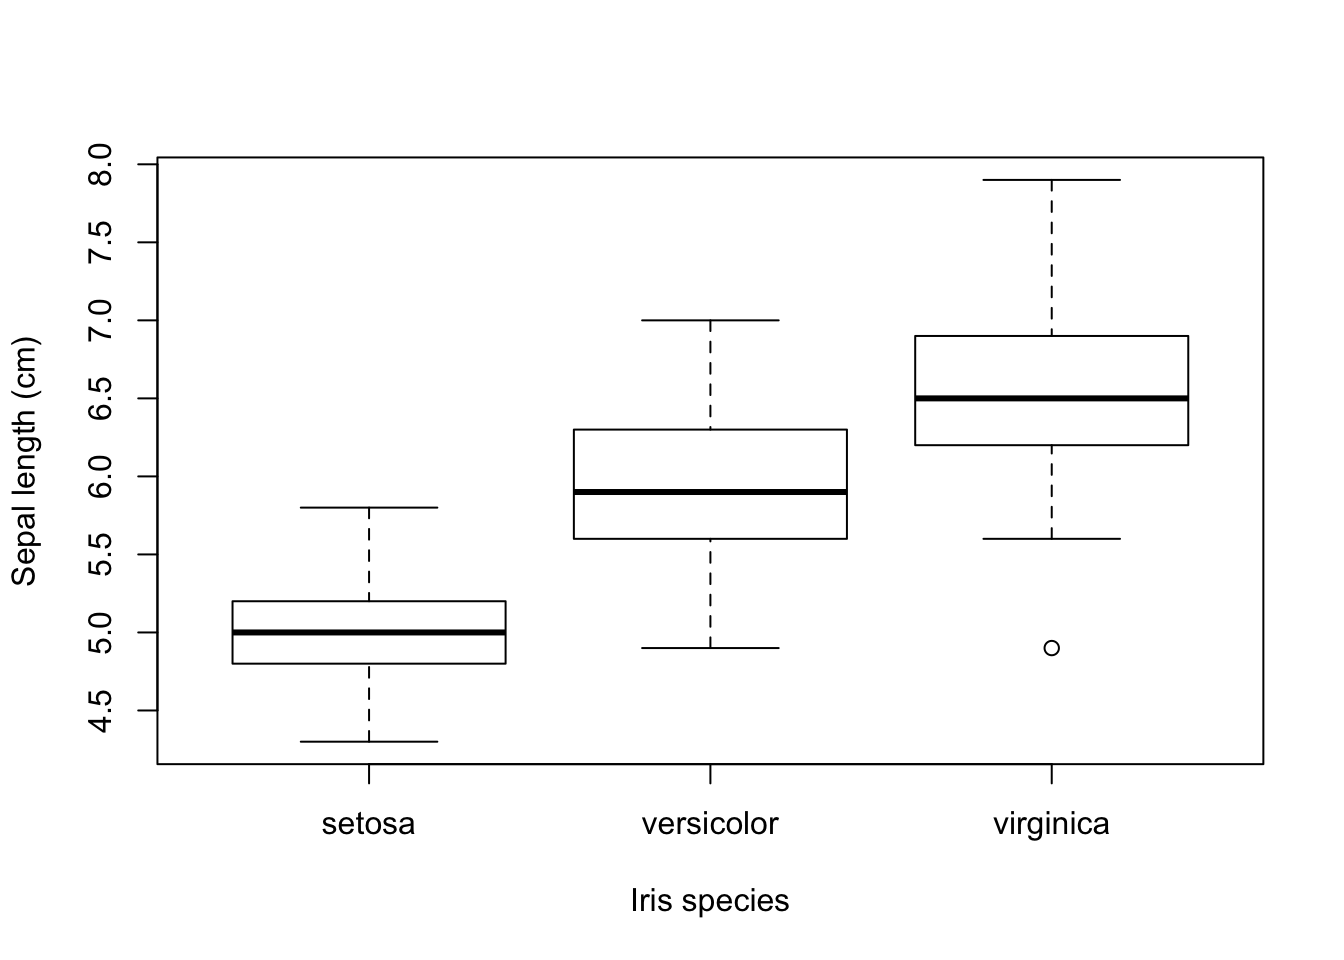
\includegraphics{davur_ebook_files/figure-latex/boxplot_sepal_length-1.pdf}

Now suppose I want to get the data from \emph{virginica} plants that have a Sepal length smaller than the largest Sepal length of \emph{setosa} plants?
First of course we'll need the maximum of the \emph{setosa} plants:

\begin{Shaded}
\begin{Highlighting}[]
\NormalTok{max.setosa <-}\StringTok{ }\KeywordTok{max}\NormalTok{(iris[iris}\OperatorTok{$}\NormalTok{Species }\OperatorTok{==}\StringTok{ "setosa"}\NormalTok{, }\StringTok{"Sepal.Length"}\NormalTok{])}
\NormalTok{max.setosa}
\end{Highlighting}
\end{Shaded}

\begin{verbatim}
## [1] 5.8
\end{verbatim}

Which plant is it? Let's use the subset function to find out.

\begin{Shaded}
\begin{Highlighting}[]
\KeywordTok{subset}\NormalTok{(}\DataTypeTok{x =}\NormalTok{ iris,}
       \DataTypeTok{subset =}\NormalTok{ (Species }\OperatorTok{==}\StringTok{ "setosa"} \OperatorTok{&}\StringTok{ }\NormalTok{Sepal.Length }\OperatorTok{==}\StringTok{ }\NormalTok{max.setosa))}
\end{Highlighting}
\end{Shaded}

\begin{verbatim}
##    Sepal.Length Sepal.Width Petal.Length Petal.Width Species
## 15          5.8           4          1.2         0.2  setosa
\end{verbatim}

Now filter out the \emph{virginica} plants that have a Sepal length smaller than this value. I'll show two approaches, one with logical indexing and one with \texttt{subset}

\begin{Shaded}
\begin{Highlighting}[]
\CommentTok{##get a logical for small plants}
\NormalTok{logi.small.sepal <-}\StringTok{ }\NormalTok{iris}\OperatorTok{$}\NormalTok{Sepal.Length }\OperatorTok{<}\StringTok{ }\NormalTok{max.setosa}
\NormalTok{logi.small.sepal}
\end{Highlighting}
\end{Shaded}

\begin{verbatim}
##   [1]  TRUE  TRUE  TRUE  TRUE  TRUE  TRUE  TRUE  TRUE  TRUE  TRUE  TRUE
##  [12]  TRUE  TRUE  TRUE FALSE  TRUE  TRUE  TRUE  TRUE  TRUE  TRUE  TRUE
##  [23]  TRUE  TRUE  TRUE  TRUE  TRUE  TRUE  TRUE  TRUE  TRUE  TRUE  TRUE
##  [34]  TRUE  TRUE  TRUE  TRUE  TRUE  TRUE  TRUE  TRUE  TRUE  TRUE  TRUE
##  [45]  TRUE  TRUE  TRUE  TRUE  TRUE  TRUE FALSE FALSE FALSE  TRUE FALSE
##  [56]  TRUE FALSE  TRUE FALSE  TRUE  TRUE FALSE FALSE FALSE  TRUE FALSE
##  [67]  TRUE FALSE FALSE  TRUE FALSE FALSE FALSE FALSE FALSE FALSE FALSE
##  [78] FALSE FALSE  TRUE  TRUE  TRUE FALSE FALSE  TRUE FALSE FALSE FALSE
##  [89]  TRUE  TRUE  TRUE FALSE FALSE  TRUE  TRUE  TRUE  TRUE FALSE  TRUE
## [100]  TRUE FALSE FALSE FALSE FALSE FALSE FALSE  TRUE FALSE FALSE FALSE
## [111] FALSE FALSE FALSE  TRUE FALSE FALSE FALSE FALSE FALSE FALSE FALSE
## [122]  TRUE FALSE FALSE FALSE FALSE FALSE FALSE FALSE FALSE FALSE FALSE
## [133] FALSE FALSE FALSE FALSE FALSE FALSE FALSE FALSE FALSE FALSE FALSE
## [144] FALSE FALSE FALSE FALSE FALSE FALSE FALSE
\end{verbatim}

\begin{Shaded}
\begin{Highlighting}[]
\CommentTok{##get a logical for virginica plants}
\NormalTok{logi.virginica <-}\StringTok{ }\NormalTok{iris}\OperatorTok{$}\NormalTok{Species }\OperatorTok{==}\StringTok{ "virginica"}
\NormalTok{logi.virginica}
\end{Highlighting}
\end{Shaded}

\begin{verbatim}
##   [1] FALSE FALSE FALSE FALSE FALSE FALSE FALSE FALSE FALSE FALSE FALSE
##  [12] FALSE FALSE FALSE FALSE FALSE FALSE FALSE FALSE FALSE FALSE FALSE
##  [23] FALSE FALSE FALSE FALSE FALSE FALSE FALSE FALSE FALSE FALSE FALSE
##  [34] FALSE FALSE FALSE FALSE FALSE FALSE FALSE FALSE FALSE FALSE FALSE
##  [45] FALSE FALSE FALSE FALSE FALSE FALSE FALSE FALSE FALSE FALSE FALSE
##  [56] FALSE FALSE FALSE FALSE FALSE FALSE FALSE FALSE FALSE FALSE FALSE
##  [67] FALSE FALSE FALSE FALSE FALSE FALSE FALSE FALSE FALSE FALSE FALSE
##  [78] FALSE FALSE FALSE FALSE FALSE FALSE FALSE FALSE FALSE FALSE FALSE
##  [89] FALSE FALSE FALSE FALSE FALSE FALSE FALSE FALSE FALSE FALSE FALSE
## [100] FALSE  TRUE  TRUE  TRUE  TRUE  TRUE  TRUE  TRUE  TRUE  TRUE  TRUE
## [111]  TRUE  TRUE  TRUE  TRUE  TRUE  TRUE  TRUE  TRUE  TRUE  TRUE  TRUE
## [122]  TRUE  TRUE  TRUE  TRUE  TRUE  TRUE  TRUE  TRUE  TRUE  TRUE  TRUE
## [133]  TRUE  TRUE  TRUE  TRUE  TRUE  TRUE  TRUE  TRUE  TRUE  TRUE  TRUE
## [144]  TRUE  TRUE  TRUE  TRUE  TRUE  TRUE  TRUE
\end{verbatim}

\begin{Shaded}
\begin{Highlighting}[]
\CommentTok{##combine the two via a boolean operation}
\NormalTok{logi.both <-}\StringTok{ }\NormalTok{logi.small.sepal }\OperatorTok{&}\StringTok{ }\NormalTok{logi.virginica}
\NormalTok{logi.both}
\end{Highlighting}
\end{Shaded}

\begin{verbatim}
##   [1] FALSE FALSE FALSE FALSE FALSE FALSE FALSE FALSE FALSE FALSE FALSE
##  [12] FALSE FALSE FALSE FALSE FALSE FALSE FALSE FALSE FALSE FALSE FALSE
##  [23] FALSE FALSE FALSE FALSE FALSE FALSE FALSE FALSE FALSE FALSE FALSE
##  [34] FALSE FALSE FALSE FALSE FALSE FALSE FALSE FALSE FALSE FALSE FALSE
##  [45] FALSE FALSE FALSE FALSE FALSE FALSE FALSE FALSE FALSE FALSE FALSE
##  [56] FALSE FALSE FALSE FALSE FALSE FALSE FALSE FALSE FALSE FALSE FALSE
##  [67] FALSE FALSE FALSE FALSE FALSE FALSE FALSE FALSE FALSE FALSE FALSE
##  [78] FALSE FALSE FALSE FALSE FALSE FALSE FALSE FALSE FALSE FALSE FALSE
##  [89] FALSE FALSE FALSE FALSE FALSE FALSE FALSE FALSE FALSE FALSE FALSE
## [100] FALSE FALSE FALSE FALSE FALSE FALSE FALSE  TRUE FALSE FALSE FALSE
## [111] FALSE FALSE FALSE  TRUE FALSE FALSE FALSE FALSE FALSE FALSE FALSE
## [122]  TRUE FALSE FALSE FALSE FALSE FALSE FALSE FALSE FALSE FALSE FALSE
## [133] FALSE FALSE FALSE FALSE FALSE FALSE FALSE FALSE FALSE FALSE FALSE
## [144] FALSE FALSE FALSE FALSE FALSE FALSE FALSE
\end{verbatim}

\begin{Shaded}
\begin{Highlighting}[]
\CommentTok{##use it as a selector on the rows of the iris DF}
\NormalTok{iris[logi.both, ]}
\end{Highlighting}
\end{Shaded}

\begin{verbatim}
##     Sepal.Length Sepal.Width Petal.Length Petal.Width   Species
## 107          4.9         2.5          4.5         1.7 virginica
## 114          5.7         2.5          5.0         2.0 virginica
## 122          5.6         2.8          4.9         2.0 virginica
\end{verbatim}

Of course, you will usually perform this selection in one statement, but the operations carried out by R will be exactly the same (but without creating any variables of course):

\begin{Shaded}
\begin{Highlighting}[]
\NormalTok{iris[iris}\OperatorTok{$}\NormalTok{Sepal.Length }\OperatorTok{<}\StringTok{ }\NormalTok{max.setosa }\OperatorTok{&}\StringTok{ }\NormalTok{iris}\OperatorTok{$}\NormalTok{Species }\OperatorTok{==}\StringTok{ "virginica"}\NormalTok{, ]}
\end{Highlighting}
\end{Shaded}

\begin{verbatim}
##     Sepal.Length Sepal.Width Petal.Length Petal.Width   Species
## 107          4.9         2.5          4.5         1.7 virginica
## 114          5.7         2.5          5.0         2.0 virginica
## 122          5.6         2.8          4.9         2.0 virginica
\end{verbatim}

The function \texttt{subset} will do the same behind the scenes, but your code may be more to your liking:

\begin{Shaded}
\begin{Highlighting}[]
\KeywordTok{subset}\NormalTok{(}\DataTypeTok{x =}\NormalTok{ iris,}
       \DataTypeTok{subset =}\NormalTok{ Sepal.Length }\OperatorTok{<}\StringTok{ }\NormalTok{max.setosa }\OperatorTok{&}\StringTok{ }\NormalTok{Species }\OperatorTok{==}\StringTok{ "virginica"}\NormalTok{)}
\end{Highlighting}
\end{Shaded}

\begin{verbatim}
##     Sepal.Length Sepal.Width Petal.Length Petal.Width   Species
## 107          4.9         2.5          4.5         1.7 virginica
## 114          5.7         2.5          5.0         2.0 virginica
## 122          5.6         2.8          4.9         2.0 virginica
\end{verbatim}

By the way, \textbf{beware to use only one boolean and: \&, not \&\&}. This will not give an error but only an empty result set

\begin{Shaded}
\begin{Highlighting}[]
\KeywordTok{subset}\NormalTok{(}\DataTypeTok{x =}\NormalTok{ iris,}
       \DataTypeTok{subset =}\NormalTok{ Sepal.Length }\OperatorTok{<}\StringTok{ }\NormalTok{max.setosa }\OperatorTok{&&}\StringTok{ }\NormalTok{Species }\OperatorTok{==}\StringTok{ "virginica"}\NormalTok{)}
\end{Highlighting}
\end{Shaded}

\begin{verbatim}
## [1] Sepal.Length Sepal.Width  Petal.Length Petal.Width  Species     
## <0 rows> (or 0-length row.names)
\end{verbatim}

\begin{quote}
\& and \&\& indicate logical AND and \textbar{} and \textbar{}\textbar{} indicate logical OR. The shorter form performs elementwise comparisons in much the same way as arithmetic operators. The longer form evaluates left to right examining only the first element of each vector. Evaluation proceeds only until the result is determined. The longer form is appropriate for programming control-flow and typically preferred in if clauses.
\end{quote}

Can you figure out why using \texttt{\&\&} would give an empty set in the above case?

See \href{http://stat.ethz.ch/R-manual/R-patched/library/base/html/Logic.html}{The R manual} for details.

\hypertarget{apply}{%
\subsection{Apply}\label{apply}}

Consider the \texttt{women} dataset, holding height and weight of a population sample of 15 women:

\begin{Shaded}
\begin{Highlighting}[]
\NormalTok{knitr}\OperatorTok{::}\KeywordTok{kable}\NormalTok{(women)}
\end{Highlighting}
\end{Shaded}

\begin{tabular}{r|r|r}
\hline
height & weight & bmi\\
\hline
58 & 115 & 24.03\\
\hline
59 & 117 & 23.63\\
\hline
60 & 120 & 23.43\\
\hline
61 & 123 & 23.24\\
\hline
62 & 126 & 23.04\\
\hline
63 & 129 & 22.85\\
\hline
64 & 132 & 22.66\\
\hline
65 & 135 & 22.46\\
\hline
66 & 139 & 22.43\\
\hline
67 & 142 & 22.24\\
\hline
68 & 146 & 22.20\\
\hline
69 & 150 & 22.15\\
\hline
70 & 154 & 22.09\\
\hline
71 & 159 & 22.17\\
\hline
72 & 164 & 22.24\\
\hline
\end{tabular}

To calculate the average height and the average weight of this sample, one could of course simply do

\begin{Shaded}
\begin{Highlighting}[]
\KeywordTok{with}\NormalTok{(women, \{}
    \KeywordTok{print}\NormalTok{(}\KeywordTok{mean}\NormalTok{(height))}
    \KeywordTok{print}\NormalTok{(}\KeywordTok{mean}\NormalTok{(weight))}
\NormalTok{\})}
\end{Highlighting}
\end{Shaded}

\begin{verbatim}
## [1] 65
## [1] 136.7
\end{verbatim}

However, when your dataset has (a lot) more columns, repeating this will be quite tedious\ldots{}unless you use a \texttt{for} loop

\begin{Shaded}
\begin{Highlighting}[]
\ControlFlowTok{for}\NormalTok{ (i }\ControlFlowTok{in} \DecValTok{1}\OperatorTok{:}\KeywordTok{length}\NormalTok{(women)) \{}
    \KeywordTok{print}\NormalTok{(}\KeywordTok{mean}\NormalTok{(women[,i]))}
\NormalTok{\}}
\end{Highlighting}
\end{Shaded}

\begin{verbatim}
## [1] 65
## [1] 136.7
## [1] 22.72
\end{verbatim}

Enter \texttt{apply()}, a very nice function to do this in a handy one-liner

\begin{Shaded}
\begin{Highlighting}[]
\KeywordTok{apply}\NormalTok{(}\DataTypeTok{X =}\NormalTok{ women, }\DataTypeTok{MARGIN =} \DecValTok{2}\NormalTok{, }\DataTypeTok{FUN =}\NormalTok{ mean)}
\end{Highlighting}
\end{Shaded}

\begin{verbatim}
## height weight    bmi 
##  65.00 136.73  22.72
\end{verbatim}

The arguments I supplied to \texttt{apply}have the following purpose:

\begin{enumerate}
\def\labelenumi{\arabic{enumi}.}
\tightlist
\item
  \texttt{X\ =\ women} specifies the data to be processed
\item
  \texttt{MARGIN\ =\ 2} specifies wether columns or rows shoud be processed; 1 = rows and 2 = columns
\item
  \texttt{FUN\ =\ mean} speciefies the function to be applied to the given dataframe
\end{enumerate}

Not only gives apply the the exact same result (of course, duh), but this approach has several advantages:

\begin{itemize}
\tightlist
\item
  \texttt{apply} returns a named vector where the elements are named the same as the corresponding columns of the original dataframe
\item
  \texttt{apply} is computationally more efficient than the other approaches
\item
  it requires less code; a good programmer types as little as possible - except for Java programmers of course :-)
\end{itemize}

If you really have strongh feelings about typing no more than strictly required, you can of course also omit the method parameters:

\begin{Shaded}
\begin{Highlighting}[]
\KeywordTok{apply}\NormalTok{(women, }\DecValTok{2}\NormalTok{, mean)}
\end{Highlighting}
\end{Shaded}

\begin{verbatim}
## height weight    bmi 
##  65.00 136.73  22.72
\end{verbatim}

But if you are just starting out with R, I suggest you invest those few character strokes for readability later on.

The above example dealt with columns. For instance, if you want to calculate the BMI of these women, you'll need to target the rows.
The BMI formula is
\[weight/height^2*703\]

where weight is in pounds and height is in inches.

This formula is implemented in the following function.

\begin{Shaded}
\begin{Highlighting}[]
\NormalTok{bmi <-}\StringTok{ }\ControlFlowTok{function}\NormalTok{(height, weight) \{}
\NormalTok{    (weight }\OperatorTok{/}\StringTok{ }\NormalTok{height}\OperatorTok{^}\DecValTok{2}\NormalTok{) }\OperatorTok{*}\StringTok{ }\DecValTok{703}
\NormalTok{\}}
\KeywordTok{bmi}\NormalTok{(}\DecValTok{65}\NormalTok{, }\DecValTok{150}\NormalTok{)}
\end{Highlighting}
\end{Shaded}

\begin{verbatim}
## [1] 24.96
\end{verbatim}

You can also apply the formula to the \texttt{women} dataset:

\begin{Shaded}
\begin{Highlighting}[]
\NormalTok{women}\OperatorTok{$}\NormalTok{bmi1 <-}\StringTok{ }\KeywordTok{apply}\NormalTok{(}
    \DataTypeTok{X =}\NormalTok{ women, }
    \DataTypeTok{MARGIN =} \DecValTok{1}\NormalTok{, }
    \DataTypeTok{FUN =} \ControlFlowTok{function}\NormalTok{(x)\{(x[}\DecValTok{2}\NormalTok{] }\OperatorTok{/}\StringTok{ }\NormalTok{x[}\DecValTok{1}\NormalTok{]}\OperatorTok{^}\DecValTok{2}\NormalTok{) }\OperatorTok{*}\StringTok{ }\DecValTok{703}\NormalTok{\})}
\KeywordTok{head}\NormalTok{(women, }\DataTypeTok{n =} \DecValTok{4}\NormalTok{)}
\end{Highlighting}
\end{Shaded}

\begin{verbatim}
##   height weight   bmi  bmi1
## 1     58    115 24.03 24.03
## 2     59    117 23.63 23.63
## 3     60    120 23.43 23.43
## 4     61    123 23.24 23.24
\end{verbatim}

if you like to use your own formula (it's always a good idea to write logic only once and reuse it in different places), you'll still need to wrap it inside an anonymous function call:

\begin{Shaded}
\begin{Highlighting}[]
\NormalTok{women}\OperatorTok{$}\NormalTok{bmi2 <-}\StringTok{ }\KeywordTok{apply}\NormalTok{(}
    \DataTypeTok{X =}\NormalTok{ women, }
    \DataTypeTok{MARGIN =} \DecValTok{1}\NormalTok{, }
    \DataTypeTok{FUN =} \ControlFlowTok{function}\NormalTok{(x)\{}\KeywordTok{bmi}\NormalTok{(x[}\DecValTok{1}\NormalTok{], x[}\DecValTok{2}\NormalTok{])\})}
\KeywordTok{head}\NormalTok{(women, }\DataTypeTok{n =} \DecValTok{4}\NormalTok{)}
\end{Highlighting}
\end{Shaded}

\begin{verbatim}
##   height weight   bmi  bmi1  bmi2
## 1     58    115 24.03 24.03 24.03
## 2     59    117 23.63 23.63 23.63
## 3     60    120 23.43 23.43 23.43
## 4     61    123 23.24 23.24 23.24
\end{verbatim}

\hypertarget{embeddeddf}{%
\subsection{Processing Embedded Dataframes}\label{embeddeddf}}

Suppose you have imported some data that has a structure like this

\begin{Shaded}
\begin{Highlighting}[]
\NormalTok{genes <-}\StringTok{ }\KeywordTok{c}\NormalTok{(}\StringTok{"gene A"}\NormalTok{, }\StringTok{"gene B"}\NormalTok{, }\StringTok{"gene C"}\NormalTok{, }\StringTok{"gene D"}\NormalTok{)}
\NormalTok{positions <-}\StringTok{ }\KeywordTok{c}\NormalTok{(}\StringTok{"chr01:128757:129667"}\NormalTok{, }
               \StringTok{"chr01:366389:486990"}\NormalTok{,}
               \StringTok{"chr02:8986463:9100856"}\NormalTok{,}
               \StringTok{"chr03:53536:87201"}\NormalTok{)}
\NormalTok{my.genome <-}\StringTok{ }\KeywordTok{data.frame}\NormalTok{(}\DataTypeTok{gene =}\NormalTok{ genes, }\DataTypeTok{position =}\NormalTok{ positions)}
\NormalTok{my.genome}
\end{Highlighting}
\end{Shaded}

\begin{verbatim}
##     gene              position
## 1 gene A   chr01:128757:129667
## 2 gene B   chr01:366389:486990
## 3 gene C chr02:8986463:9100856
## 4 gene D     chr03:53536:87201
\end{verbatim}

The problem here is that the second column, \texttt{positions}, of type \texttt{character}, actually holds three different variables: the chromosome identifyer, the start position and the stop position on the chromosome. To be able to perform analyses of chromosomal contents, or positional contexts, we will need to split this column into separate columns, each holding exactly one variable of the correct type (\texttt{factor}, \texttt{integer} and \texttt{integer}).

When I first encountered this type of problem (it is a \emph{challenge} actually, some teachers would object, not a \emph{problem}\ldots{}), my first thought was ``easy, simply apply a split and bind as three columns''.

Let's have a look at how the \texttt{strsplit} function works in splitting strings

\begin{Shaded}
\begin{Highlighting}[]
\KeywordTok{strsplit}\NormalTok{(}\DataTypeTok{x =}\NormalTok{ positions[}\DecValTok{1}\OperatorTok{:}\DecValTok{2}\NormalTok{], }\DataTypeTok{split =} \StringTok{":"}\NormalTok{)}
\end{Highlighting}
\end{Shaded}

\begin{verbatim}
## [[1]]
## [1] "chr01"  "128757" "129667"
## 
## [[2]]
## [1] "chr01"  "366389" "486990"
\end{verbatim}

As you can see, strsplit generates a list of vectors, with each vector corresponding to the string at the same index of the original character vector.
So, easy, I thought. Simply assign these elements to three new columns of the original dataframe (assuming every split character results in a vector of three). I first created the columns, defined my splitter function and then used apply to get the job done

\begin{Shaded}
\begin{Highlighting}[]
\CommentTok{## create columns}
\NormalTok{my.genome[, }\KeywordTok{c}\NormalTok{(}\StringTok{"chromosome"}\NormalTok{, }\StringTok{"start"}\NormalTok{, }\StringTok{"stop"}\NormalTok{)] <-}\StringTok{ }\OtherTok{NA}
\CommentTok{## define splitter function}
\NormalTok{loc.splitter <-}\StringTok{ }\ControlFlowTok{function}\NormalTok{(x) \{}
    \CommentTok{## strsplit returns a list!}
    \KeywordTok{strsplit}\NormalTok{(x[}\StringTok{"position"}\NormalTok{], }\StringTok{":"}\NormalTok{)[[}\DecValTok{1}\NormalTok{]]}
\NormalTok{\}}
\CommentTok{## use apply to fill the columns}
\NormalTok{my.genome[, }\DecValTok{3}\OperatorTok{:}\DecValTok{5}\NormalTok{] <-}\StringTok{ }\KeywordTok{apply}\NormalTok{(}\DataTypeTok{X =}\NormalTok{ my.genome,}
                          \DataTypeTok{MARGIN =} \DecValTok{1}\NormalTok{,}
                          \DataTypeTok{FUN =}\NormalTok{ loc.splitter)}
\NormalTok{my.genome}
\end{Highlighting}
\end{Shaded}

\begin{verbatim}
##     gene              position chromosome   start    stop
## 1 gene A   chr01:128757:129667      chr01  366389 9100856
## 2 gene B   chr01:366389:486990     128757  486990   chr03
## 3 gene C chr02:8986463:9100856     129667   chr02   53536
## 4 gene D     chr03:53536:87201      chr01 8986463   87201
\end{verbatim}

Whoa, what happened here?! This was not what I had in mind. Can you figure out what happened?

\ldots{}

I did figure it out (eventually\ldots{}). The applied function returned three elements at a time, and I had apply fill three columns of my dataframe. And that is exactly what R did, fill the three columns, but not by row but by column! Have a look at the output from apply and you can see:

\begin{Shaded}
\begin{Highlighting}[]
\KeywordTok{apply}\NormalTok{(}\DataTypeTok{X =}\NormalTok{ my.genome,}
      \DataTypeTok{MARGIN =} \DecValTok{1}\NormalTok{,}
      \DataTypeTok{FUN =}\NormalTok{ loc.splitter)}
\end{Highlighting}
\end{Shaded}

\begin{verbatim}
##      [,1]     [,2]     [,3]      [,4]   
## [1,] "chr01"  "chr01"  "chr02"   "chr03"
## [2,] "128757" "366389" "8986463" "53536"
## [3,] "129667" "486990" "9100856" "87201"
\end{verbatim}

Fortunately, R has a function to transpose this kind of structure (a matrix actually): the \texttt{t()} function, so that is what I did:

\begin{Shaded}
\begin{Highlighting}[]
\NormalTok{my.genome[, }\DecValTok{3}\OperatorTok{:}\DecValTok{5}\NormalTok{] <-}\StringTok{ }\KeywordTok{t}\NormalTok{(}\KeywordTok{apply}\NormalTok{(}\DataTypeTok{X =}\NormalTok{ my.genome,}
                            \DataTypeTok{MARGIN =} \DecValTok{1}\NormalTok{,}
                            \DataTypeTok{FUN =}\NormalTok{ loc.splitter))}
\NormalTok{my.genome}
\end{Highlighting}
\end{Shaded}

\begin{verbatim}
##     gene              position chromosome   start    stop
## 1 gene A   chr01:128757:129667      chr01  128757  129667
## 2 gene B   chr01:366389:486990      chr01  366389  486990
## 3 gene C chr02:8986463:9100856      chr02 8986463 9100856
## 4 gene D     chr03:53536:87201      chr03   53536   87201
\end{verbatim}

Yeah, that's what I'm talking about! (Feeling very happy with myself\ldots{}until I googled this problem). I found out there are a gazillion solutions to this problem, but only one of them is very very simple, because it uses a function you know really well: \texttt{read.table}, but not with the \texttt{file\ =} argument but with \texttt{text\ =}:

\begin{Shaded}
\begin{Highlighting}[]
\NormalTok{my.genome <-}\StringTok{ }\KeywordTok{data.frame}\NormalTok{(}\DataTypeTok{gene =}\NormalTok{ genes, }\DataTypeTok{position =}\NormalTok{ positions)}
\NormalTok{my.genome <-}\StringTok{ }\KeywordTok{cbind}\NormalTok{(}
\NormalTok{    my.genome,}
    \KeywordTok{read.table}\NormalTok{(}
        \DataTypeTok{text =} \KeywordTok{as.character}\NormalTok{(my.genome}\OperatorTok{$}\NormalTok{position),}
        \DataTypeTok{sep =} \StringTok{":"}\NormalTok{))}
\KeywordTok{colnames}\NormalTok{(my.genome) <-}\StringTok{ }\KeywordTok{c}\NormalTok{(}\KeywordTok{colnames}\NormalTok{(my.genome)[}\DecValTok{1}\OperatorTok{:}\DecValTok{2}\NormalTok{], }\StringTok{"chr"}\NormalTok{, }\StringTok{"start"}\NormalTok{, }\StringTok{"stop"}\NormalTok{)}
\NormalTok{my.genome}
\end{Highlighting}
\end{Shaded}

\begin{verbatim}
##     gene              position   chr   start    stop
## 1 gene A   chr01:128757:129667 chr01  128757  129667
## 2 gene B   chr01:366389:486990 chr01  366389  486990
## 3 gene C chr02:8986463:9100856 chr02 8986463 9100856
## 4 gene D     chr03:53536:87201 chr03   53536   87201
\end{verbatim}

That's it. The lessons learned here:

\begin{itemize}
\tightlist
\item
  Always know that GIYF (Google Is Your Friend)
\item
  When reading tables, also those embedded within others, use \texttt{read.table}
\item
  You really learn a lot by fiddling about with data
\end{itemize}

\hypertarget{exploratory-data-analysis}{%
\chapter{Exploratory Data Analysis}\label{exploratory-data-analysis}}

\hypertarget{introduction-1}{%
\section{Introduction}\label{introduction-1}}

This chapter introduces you to the concept of Exploratory Data Analysis (EDA). In EDA a dataset is analysed with the goal of assessing its main characteristics, including its quality and usablity for subsequent statistical modelling and analysis. Data summary techniques and visualizations ore used in an EDA. There is no fixed set of activities; each dataset poses its own questions and challenges.

Datasets are often expensive and time-consuming to collect, and therefore they are ususally collected with a specific goal in mind. The EDA you perform should always be with this goal on the horizon: is the dataset of sufficient quality to answer the scientific questions for which they were collected?

\hypertarget{eda-outline}{%
\subsubsection*{EDA outline}\label{eda-outline}}
\addcontentsline{toc}{subsubsection}{EDA outline}

An EDA therefore may include:

\begin{itemize}
\tightlist
\item
  \textbf{Dataset description}: how were they collected, what data types do the variables have, what are the units and physical quantities, how are missing data encoded, etc.
\item
  \textbf{Data summary}: number of cases, number of variables, basic statistical description (i.e.~mean, median, sd etc.), variable distributions (normal or not, outliers, missing data, skewed distributions)
\item
  \textbf{Visual summaries} using boxplots, histograms, density plots.
\item
  \textbf{Recoding or transformations of variables} may be required to get better results (e.g.~from numeric to factor or vice versa, or log transformation of exponential data)
\item
  \textbf{Exploration of variable relations/covariance}. It is always interesting to know about correlations between variables, but this is especially the case when you have a \emph{dependent} variable for which you wish to build a statistical model in a later stage of your analysis.
\end{itemize}

Note that your EDA results should \emph{always} be accompanied by text that describes your results and discusses the implications of them. your figures should be well annotated with a caption and legend if relevant. An EDA is \emph{not} a publication, but it will usually have a short introduction, a results section and a discussion. In contrast with a publication you usually \emph{do} show the code. This ensures complete transparency and reproducibility.

In this chapter I will demonstrate a short EDA on the ``Yeast dataset'' from the UCI Machine Learning repository.

It is outside the scope of this short analysis to delve too deeply in the attribute background information, but you should realise that for a real analysis this is absolutely critical: without domain knowledge the you won't have the insight to identify strange, worrying or surprising results.

\hypertarget{eda-of-the-yeast-dataset}{%
\section{EDA of the Yeast dataset}\label{eda-of-the-yeast-dataset}}

\hypertarget{introduction-2}{%
\subsection{Introduction}\label{introduction-2}}

The data were collected from the \href{https://archive.ics.uci.edu/ml/datasets/Yeast}{UCI Machine Learning website}. To ensure their continued availability the files were copied to a personal \href{https://github.com/MichielNoback/datasets/tree/master/UCI_yeast_protein_loc}{repository}.

The data were accompanied by a \emph{very} short abstract: \textbf{\emph{``Predicting the Cellular Localization Sites of Proteins''}}. The data description states there are 1484 instances, each with 8 attributes (variables) and a class label. The class label is the variable we wish to biuld a model for so this is the dependent variable.

The \emph{Attribute Information} section descibes these variables:

\begin{enumerate}
\def\labelenumi{\arabic{enumi}.}
\tightlist
\item
  Sequence Name: Accession number for the SWISS-PROT database
\item
  \texttt{mcg}: McGeoch's method for signal sequence recognition.
\item
  \texttt{gvh}: von Heijne's method for signal sequence recognition.
\item
  \texttt{alm}: Score of the ALOM membrane spanning region prediction program.
\item
  \texttt{mit}: Score of discriminant analysis of the amino acid content of the N-terminal region (20 residues long) of mitochondrial and non-mitochondrial proteins.
\item
  \texttt{erl}: Presence of ``HDEL'' substring (thought to act as a signal for retention in the endoplasmic reticulum lumen). Binary attribute.
\item
  \texttt{pox}: Peroxisomal targeting signal in the C-terminus.
\item
  \texttt{vac}: Score of discriminant analysis of the amino acid content of vacuolar and extracellular proteins.
\item
  \texttt{nuc}: Score of discriminant analysis of nuclear localization signals of nuclear and non-nuclear proteins.
\end{enumerate}

The sequence name is not interesting in this EDA: we are interested in patterns, not individuals. However, if there is an anomalous protein in the EDA it should be possible to retrace its origin so the identifier stays in the dataset.

There seem to be two attributes (\texttt{mcg} and \texttt{gvh}) measuring the same property - the presence of a signal sequence which is the N-terminal part of a protein signalling the cellular machinery the protein should be exported.

Very simply put, if this scoring system was perfect each of the attributes (except \texttt{mcg} and \texttt{gvh}) would unequivocally ``assign'' the protein in question to a cellular location: Cellular external matrix, membrane inserted, mitochondrial, endoplasmic reticulum lumen, peroxisomal, vacualar or nuclear.

The tenth variable in the data is the dependent or explanatory variable. The \texttt{yeast.names} file describes it like this:

\begin{verbatim}
Class Distribution. The class is the localization site. Please see Nakai &
               Kanehisa referenced above for more details.
  CYT (cytosolic or cytoskeletal)                    463
  NUC (nuclear)                                      429
  MIT (mitochondrial)                                244
  ME3 (membrane protein, no N-terminal signal)       163
  ME2 (membrane protein, uncleaved signal)            51
  ME1 (membrane protein, cleaved signal)              44
  EXC (extracellular)                                 37
  VAC (vacuolar)                                      30
  POX (peroxisomal)                                   20
  ERL (endoplasmic reticulum lumen)                    5
\end{verbatim}

This tells me the different localizations are by no means equally distributed; there is an overrepresentation of ``cytosolic or cytoskeletal'' and ``nuclear'' and a huge underrepresentation of especially endoplasmic reticulum lumen proteins.

\hypertarget{data-loading-and-prepping}{%
\subsection{Data loading and prepping}\label{data-loading-and-prepping}}

Since I am going to rerun the code in this notebook often I am going to create a local copy, and load that one.

\begin{Shaded}
\begin{Highlighting}[]
\NormalTok{file_name <-}\StringTok{ "yeast.data"}
\NormalTok{yeast_data_url <-}\StringTok{ }\KeywordTok{paste0}\NormalTok{(}\StringTok{"https://raw.githubusercontent.com/MichielNoback/datasets/master/UCI_yeast_protein_loc/"}\NormalTok{, file_name)}
\NormalTok{yeast_local_location <-}\StringTok{ }\KeywordTok{paste0}\NormalTok{(}\StringTok{"../"}\NormalTok{, file_name)}

\CommentTok{#only download if not present}
\ControlFlowTok{if}\NormalTok{ (}\OperatorTok{!}\StringTok{ }\KeywordTok{file.exists}\NormalTok{(yeast_local_location)) \{}
    \KeywordTok{download.file}\NormalTok{(}\DataTypeTok{url =}\NormalTok{ yeast_data_url, }
                  \DataTypeTok{destfile =}\NormalTok{ yeast_local_location)}
\NormalTok{\}}

\NormalTok{yeast_data <-}\StringTok{ }\KeywordTok{read.table}\NormalTok{(}\DataTypeTok{file =}\NormalTok{ yeast_local_location,}
                         \DataTypeTok{sep =} \StringTok{","}\NormalTok{,}
                         \DataTypeTok{as.is =} \DecValTok{1}\NormalTok{)}
\KeywordTok{str}\NormalTok{(yeast_data)}
\end{Highlighting}
\end{Shaded}

\begin{verbatim}
## 'data.frame':    1484 obs. of  10 variables:
##  $ V1 : chr  "ADT1_YEAST" "ADT2_YEAST" "ADT3_YEAST" "AAR2_YEAST" ...
##  $ V2 : num  0.58 0.43 0.64 0.58 0.42 0.51 0.5 0.48 0.55 0.4 ...
##  $ V3 : num  0.61 0.67 0.62 0.44 0.44 0.4 0.54 0.45 0.5 0.39 ...
##  $ V4 : num  0.47 0.48 0.49 0.57 0.48 0.56 0.48 0.59 0.66 0.6 ...
##  $ V5 : num  0.13 0.27 0.15 0.13 0.54 0.17 0.65 0.2 0.36 0.15 ...
##  $ V6 : num  0.5 0.5 0.5 0.5 0.5 0.5 0.5 0.5 0.5 0.5 ...
##  $ V7 : num  0 0 0 0 0 0.5 0 0 0 0 ...
##  $ V8 : num  0.48 0.53 0.53 0.54 0.48 0.49 0.53 0.58 0.49 0.58 ...
##  $ V9 : num  0.22 0.22 0.22 0.22 0.22 0.22 0.22 0.34 0.22 0.3 ...
##  $ V10: Factor w/ 10 levels "CYT","ERL","EXC",..: 7 7 7 8 7 1 7 8 7 1 ...
\end{verbatim}

The data seems to have been loaded correctly and, as expected since that was stated in the original data description, there are no missing data.

The column names were not defined in the data file so this will be fixed first. I will create a data frame that also holds the column desciptions. I have put the data in a small text file for easy loading and editing; the attribute descriptions copied/pasted into a text file and with find/replace converted in easy to load form, and a new \texttt{label} column added for use in plotting. There were a few occurences of the \texttt{\textquotesingle{}} character which always corrupt data import into R. They were removed.

\begin{Shaded}
\begin{Highlighting}[]
\NormalTok{attribute_info <-}\StringTok{ }\KeywordTok{read.table}\NormalTok{(}\StringTok{"data/yeast_attribute_info.txt"}\NormalTok{, }
                             \DataTypeTok{sep =} \StringTok{":"}\NormalTok{,}
                             \DataTypeTok{header =} \OtherTok{TRUE}\NormalTok{,}
                             \DataTypeTok{stringsAsFactors =} \OtherTok{FALSE}\NormalTok{)}
\CommentTok{#attach column names}
\NormalTok{(}\KeywordTok{colnames}\NormalTok{(yeast_data) <-}\StringTok{ }\NormalTok{attribute_info}\OperatorTok{$}\NormalTok{attribute)}
\end{Highlighting}
\end{Shaded}

\begin{verbatim}
##  [1] "accno" "mcg"   "gvh"   "alm"   "mit"   "erl"   "pox"   "vac"  
##  [9] "nuc"   "loc"
\end{verbatim}

To make this info easily accessible, a function is created that can be used to fetch either the description or the label.

\begin{Shaded}
\begin{Highlighting}[]
\NormalTok{get_attribute_info <-}\StringTok{ }\ControlFlowTok{function}\NormalTok{(attribute, }\DataTypeTok{resource =} \StringTok{"label"}\NormalTok{) \{}
    \ControlFlowTok{if}\NormalTok{ (}\OperatorTok{!}\StringTok{ }\NormalTok{resource }\OperatorTok\StringTok{ }\KeywordTok{c}\NormalTok{(}\StringTok{"label"}\NormalTok{, }\StringTok{"description"}\NormalTok{)) \{}
        \KeywordTok{stop}\NormalTok{(}\KeywordTok{paste0}\NormalTok{(}\StringTok{"type "}\NormalTok{, resource, }\StringTok{"is not an attribute resource"}\NormalTok{))}
\NormalTok{    \}}
    \KeywordTok{return}\NormalTok{(attribute_info[attribute_info}\OperatorTok{$}\NormalTok{attribute }\OperatorTok{==}\StringTok{ }\NormalTok{attribute, resource])}
\NormalTok{\}}

\CommentTok{#test it}
\KeywordTok{get_attribute_info}\NormalTok{(}\StringTok{"gvh"}\NormalTok{)}
\end{Highlighting}
\end{Shaded}

\begin{verbatim}
## [1] "VonHeijne signal"
\end{verbatim}

\begin{Shaded}
\begin{Highlighting}[]
\KeywordTok{get_attribute_info}\NormalTok{(}\StringTok{"accno"}\NormalTok{, }\StringTok{"description"}\NormalTok{)}
\end{Highlighting}
\end{Shaded}

\begin{verbatim}
## [1] "Accession number for the SWISS-PROT database"
\end{verbatim}

\hypertarget{data-verification}{%
\subsection{Data verification}\label{data-verification}}

The original data description stated that 1484 instances with 9 attributes + a class label are present.

\begin{Shaded}
\begin{Highlighting}[]
\KeywordTok{dim}\NormalTok{(yeast_data)}
\end{Highlighting}
\end{Shaded}

\begin{verbatim}
## [1] 1484   10
\end{verbatim}

This is correct.
No missing data are supposed to be there:

\begin{Shaded}
\begin{Highlighting}[]
\KeywordTok{sum}\NormalTok{(}\KeywordTok{complete.cases}\NormalTok{(yeast_data))}
\end{Highlighting}
\end{Shaded}

\begin{verbatim}
## [1] 1484
\end{verbatim}

Also correct.

The classes of the columns are also OK so the data is verified and found correct.

\hypertarget{attribute-summaries}{%
\subsection{Attribute summaries}\label{attribute-summaries}}

A first scan of the attributes.

\begin{Shaded}
\begin{Highlighting}[]
\KeywordTok{summary}\NormalTok{(yeast_data)}
\end{Highlighting}
\end{Shaded}

\begin{verbatim}
##     accno                mcg            gvh            alm      
##  Length:1484        Min.   :0.11   Min.   :0.13   Min.   :0.21  
##  Class :character   1st Qu.:0.41   1st Qu.:0.42   1st Qu.:0.46  
##  Mode  :character   Median :0.49   Median :0.49   Median :0.51  
##                     Mean   :0.50   Mean   :0.50   Mean   :0.50  
##                     3rd Qu.:0.58   3rd Qu.:0.57   3rd Qu.:0.55  
##                     Max.   :1.00   Max.   :1.00   Max.   :1.00  
##                                                                 
##       mit             erl             pox              vac      
##  Min.   :0.000   Min.   :0.500   Min.   :0.0000   Min.   :0.00  
##  1st Qu.:0.170   1st Qu.:0.500   1st Qu.:0.0000   1st Qu.:0.48  
##  Median :0.220   Median :0.500   Median :0.0000   Median :0.51  
##  Mean   :0.261   Mean   :0.505   Mean   :0.0075   Mean   :0.50  
##  3rd Qu.:0.320   3rd Qu.:0.500   3rd Qu.:0.0000   3rd Qu.:0.53  
##  Max.   :1.000   Max.   :1.000   Max.   :0.8300   Max.   :0.73  
##                                                                 
##       nuc             loc     
##  Min.   :0.000   CYT    :463  
##  1st Qu.:0.220   NUC    :429  
##  Median :0.220   MIT    :244  
##  Mean   :0.276   ME3    :163  
##  3rd Qu.:0.300   ME2    : 51  
##  Max.   :1.000   ME1    : 44  
##                  (Other): 90
\end{verbatim}

All these attributes seem to be in the range zero to one, except of course for the localization attribute and the accession number. This is not surprising since these attributes are all probabilities. The class distribution corresponds with the published data.

The
The \texttt{pox} (Peroxisomal) and \texttt{erl} ( ER-retention) attributes, seem to have a really strange distribution and should be investigated further.

Here are all the numeric attributes in a single panel. I chose histogram over boxplot or density plot because it is more fine-grained than boxplot and very easy to interpret.

\begin{Shaded}
\begin{Highlighting}[]
\KeywordTok{par}\NormalTok{(}\DataTypeTok{mfrow =} \KeywordTok{c}\NormalTok{(}\DecValTok{4}\NormalTok{, }\DecValTok{2}\NormalTok{))}

\ControlFlowTok{for}\NormalTok{ ( attrib }\ControlFlowTok{in} \KeywordTok{colnames}\NormalTok{(yeast_data[}\DecValTok{2}\OperatorTok{:}\DecValTok{9}\NormalTok{])) \{}
    \KeywordTok{hist}\NormalTok{(yeast_data[, attrib],}
         \DataTypeTok{main =} \OtherTok{NULL}\NormalTok{,}
         \DataTypeTok{xlab =} \KeywordTok{paste0}\NormalTok{(}\KeywordTok{get_attribute_info}\NormalTok{(attrib), }\StringTok{" (prob)"}\NormalTok{))}
\NormalTok{\}}
\end{Highlighting}
\end{Shaded}

\begin{figure}
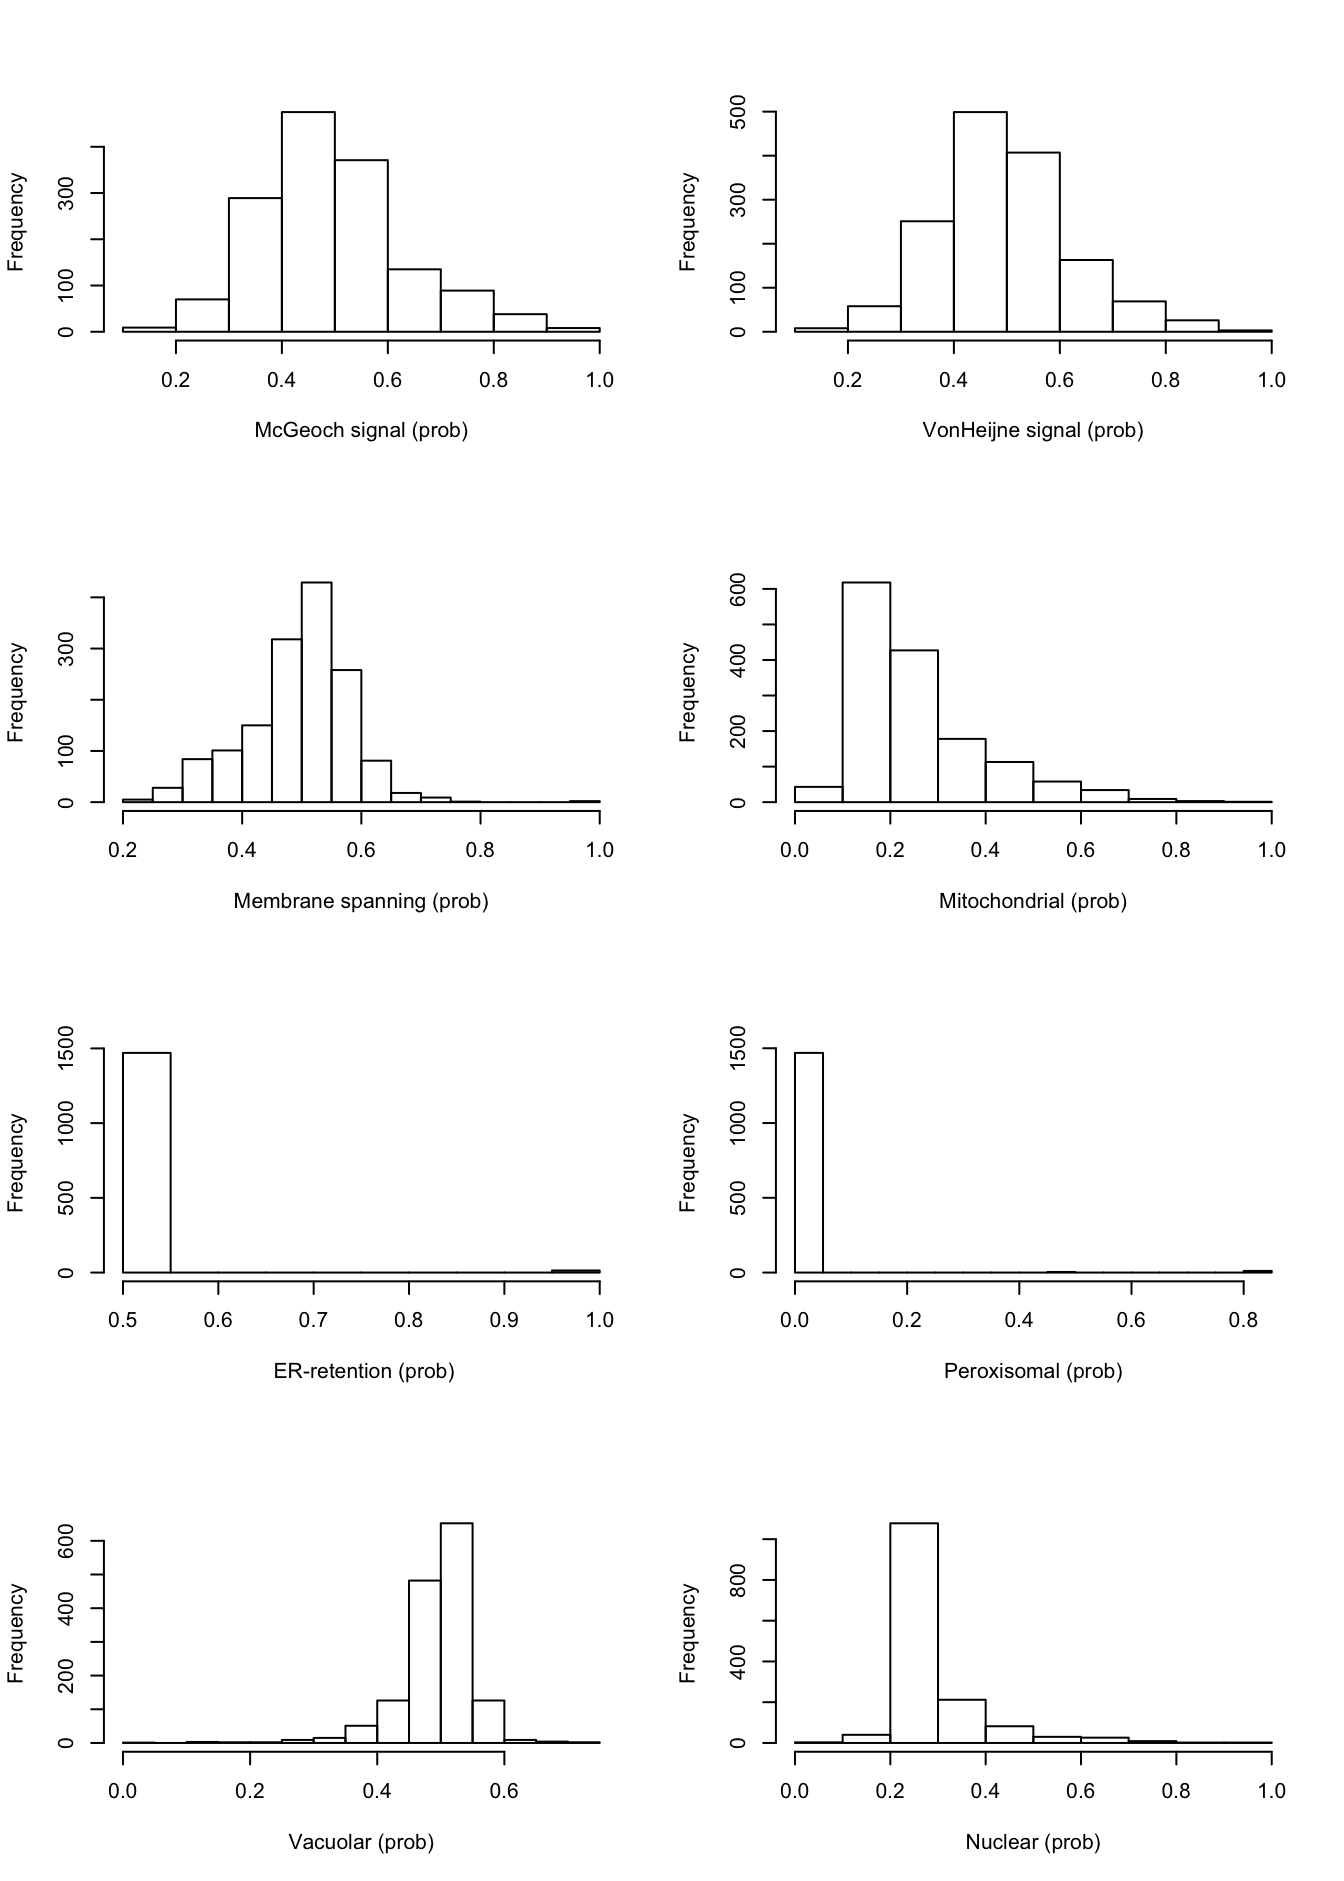
\includegraphics[width=1\linewidth]{davur_ebook_files/figure-latex/yeast-attributes-hist-1} \caption{Distributions of the numeric variables}\label{fig:yeast-attributes-hist}
\end{figure}

\begin{Shaded}
\begin{Highlighting}[]
\CommentTok{#reset par()}
\KeywordTok{par}\NormalTok{(}\DataTypeTok{mfrow =} \KeywordTok{c}\NormalTok{(}\DecValTok{1}\NormalTok{, }\DecValTok{1}\NormalTok{))}
\end{Highlighting}
\end{Shaded}

Here, it can be seen that the attributes ``ER-retention'' and ``Peroxisomal'' are pretty much uninformative, a problem probably largely caused by the low abundance of protiens in these classes. Surprisingly enough, the ``Vacuolar'' property which is also low-abundant, does not have this extreme distribution.

What is also striking is that, although these attributes are probablitities of targeting signals, none (with the exception of the two low-abundance ones) show a more or less bimodal distribution as you would naively expect.

\hypertarget{attribute-relationships}{%
\subsection{Attribute relationships}\label{attribute-relationships}}

Here is a quick scan of variable relationship, excluding the dependent variable. The \texttt{pairs()} function is used for that. I excluded \texttt{erl} and \texttt{pox} because they do not add information to the picture.

\begin{Shaded}
\begin{Highlighting}[]
\KeywordTok{pairs}\NormalTok{(yeast_data[}\KeywordTok{c}\NormalTok{(}\DecValTok{2}\NormalTok{, }\DecValTok{3}\NormalTok{, }\DecValTok{4}\NormalTok{, }\DecValTok{5}\NormalTok{, }\DecValTok{8}\NormalTok{, }\DecValTok{9}\NormalTok{)],}
      \DataTypeTok{panel =} \StringTok{"panel.smooth"}\NormalTok{,}
      \DataTypeTok{pch =} \DecValTok{20}\NormalTok{, }
      \DataTypeTok{cex =} \FloatTok{0.35}\NormalTok{,}
      \DataTypeTok{col =} \KeywordTok{rgb}\NormalTok{(}\FloatTok{0.1}\NormalTok{, }\FloatTok{0.4}\NormalTok{, }\DecValTok{1}\NormalTok{, }\DataTypeTok{alpha =} \FloatTok{0.4}\NormalTok{))}
\end{Highlighting}
\end{Shaded}

\begin{figure}
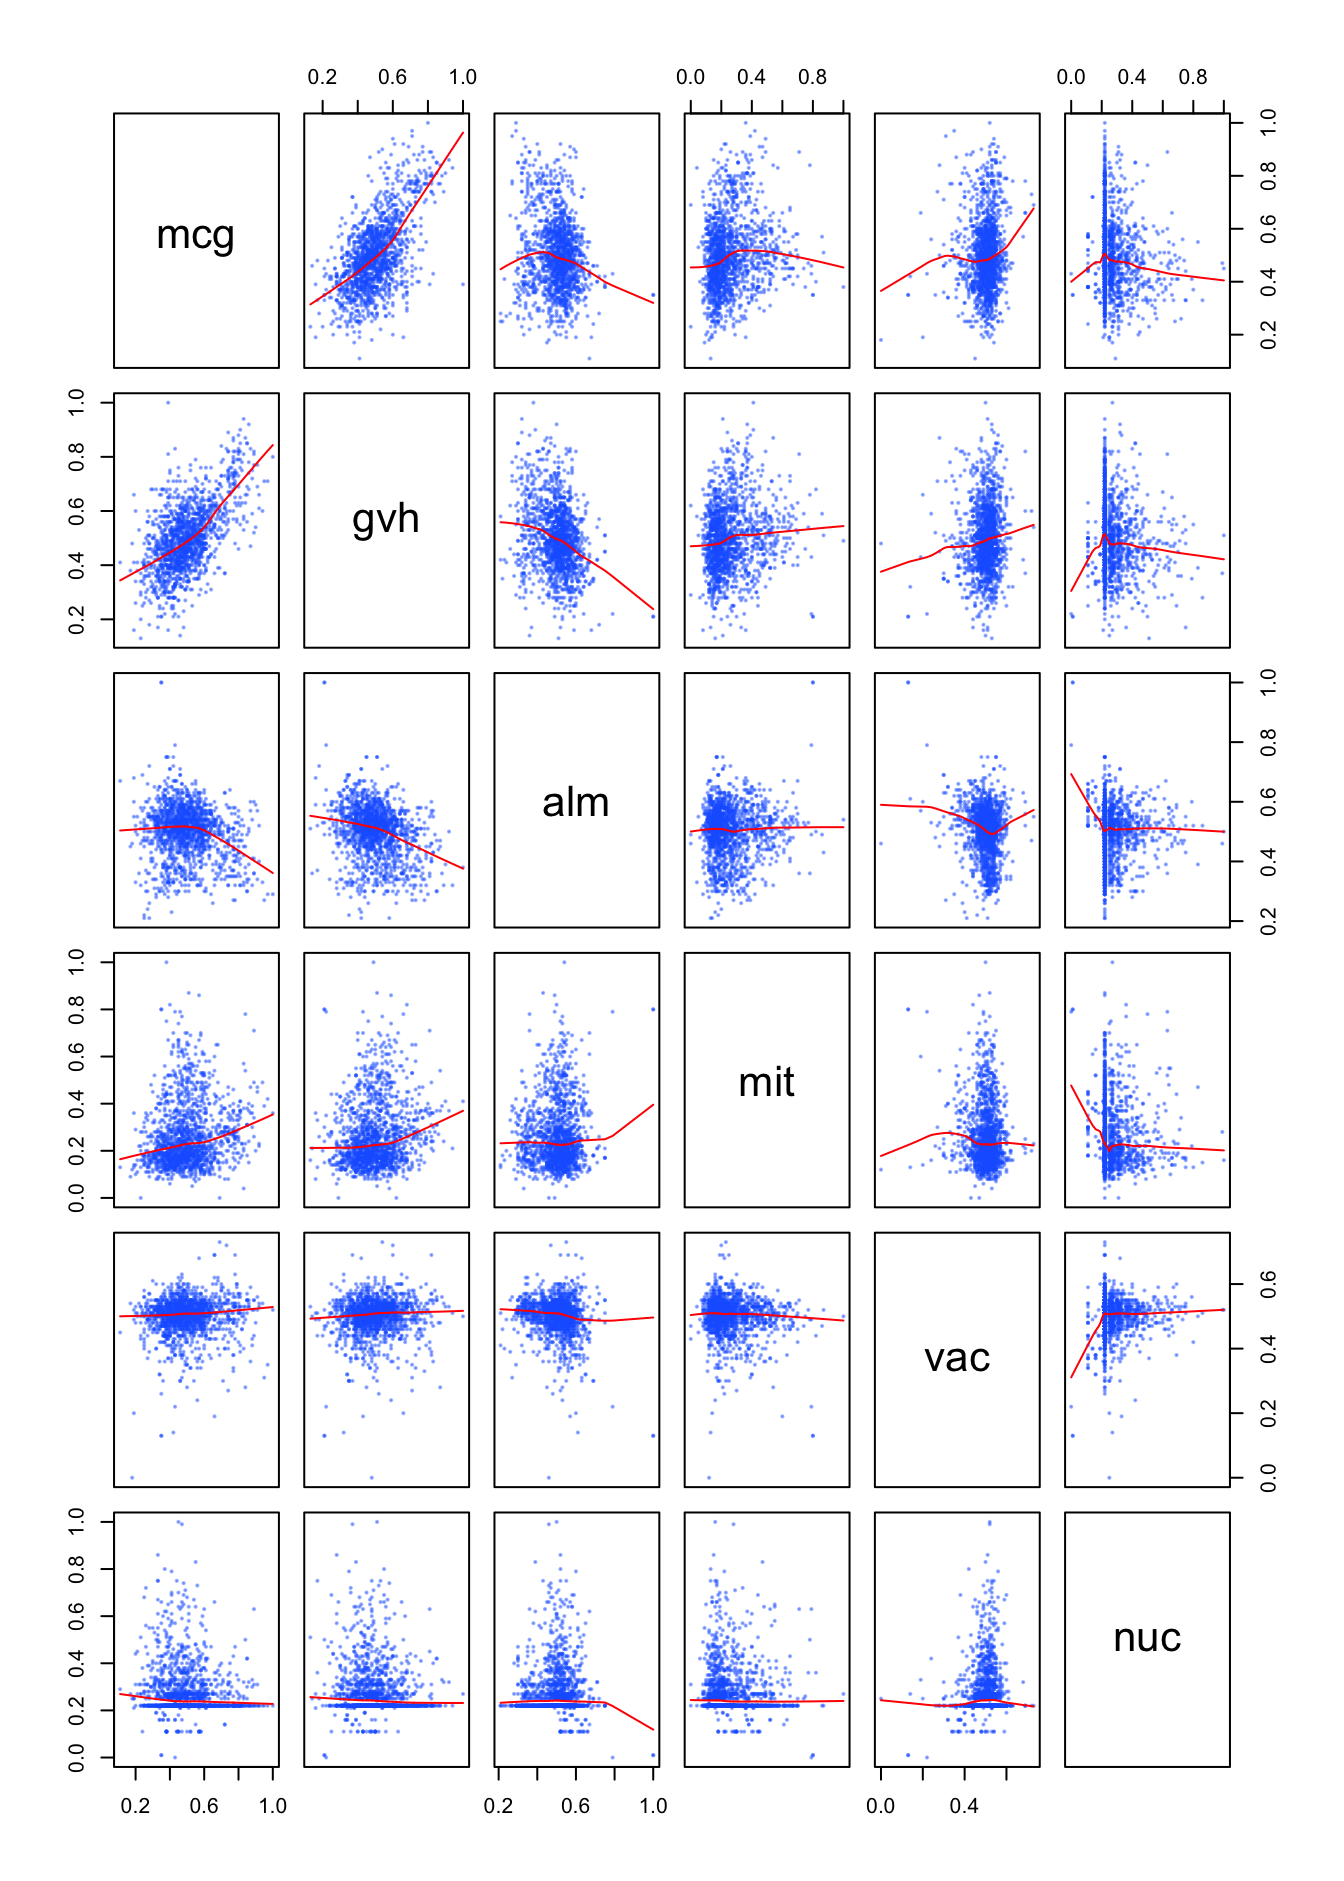
\includegraphics[width=1\linewidth]{davur_ebook_files/figure-latex/yeast-pairs-plot-1} \caption{Relations between the numeric variables}\label{fig:yeast-pairs-plot}
\end{figure}

By adding the smoother it is made clear that the only pair which shows a clear correlation is the pair \texttt{mcg} / \texttt{gvh} which actually predict the same property. Therefore it would have been very surprising indeed if they would \emph{not} have a correlation. The strength of this correlation -the \textbf{\emph{R-squared}}- is this

\begin{Shaded}
\begin{Highlighting}[]
\NormalTok{lin_mod <-}\StringTok{ }\KeywordTok{lm}\NormalTok{(yeast_data}\OperatorTok{$}\NormalTok{mcg }\OperatorTok{~}\StringTok{ }\NormalTok{yeast_data}\OperatorTok{$}\NormalTok{gvh)}
\KeywordTok{summary}\NormalTok{(lin_mod)}\OperatorTok{$}\NormalTok{r.squared}
\end{Highlighting}
\end{Shaded}

\begin{verbatim}
## [1] 0.3383
\end{verbatim}

This is not very strong.

\hypertarget{correlations-to-the-dependent-variable}{%
\subsection{Correlations to the dependent variable}\label{correlations-to-the-dependent-variable}}

As a first investigation, numeric variables are split on the location variable.

\begin{Shaded}
\begin{Highlighting}[]
\KeywordTok{library}\NormalTok{(RColorBrewer)}
\NormalTok{colors <-}\StringTok{ }\NormalTok{RColorBrewer}\OperatorTok{::}\KeywordTok{brewer.pal}\NormalTok{(}\DecValTok{8}\NormalTok{, }\DataTypeTok{name =} \StringTok{"Accent"}\NormalTok{)}
\CommentTok{#col = c("darkblue", "darkgreen", "magenta", )}
\NormalTok{col_i <-}\StringTok{ }\DecValTok{0}
\ControlFlowTok{for}\NormalTok{ (name }\ControlFlowTok{in} \KeywordTok{names}\NormalTok{(yeast_data[}\DecValTok{2}\OperatorTok{:}\DecValTok{9}\NormalTok{])) \{}
\NormalTok{    col_i <-}\StringTok{ }\NormalTok{col_i }\OperatorTok{+}\StringTok{ }\DecValTok{1}
    \KeywordTok{boxplot}\NormalTok{(yeast_data[, name] }\OperatorTok{~}\StringTok{ }\NormalTok{yeast_data}\OperatorTok{$}\NormalTok{loc,}
            \DataTypeTok{xlab =} \OtherTok{NULL}\NormalTok{,}
            \DataTypeTok{ylab =} \KeywordTok{get_attribute_info}\NormalTok{(name),}
            \DataTypeTok{col =}\NormalTok{ colors[col_i])}
\NormalTok{\}}
\end{Highlighting}
\end{Shaded}

\begin{figure}

{\centering 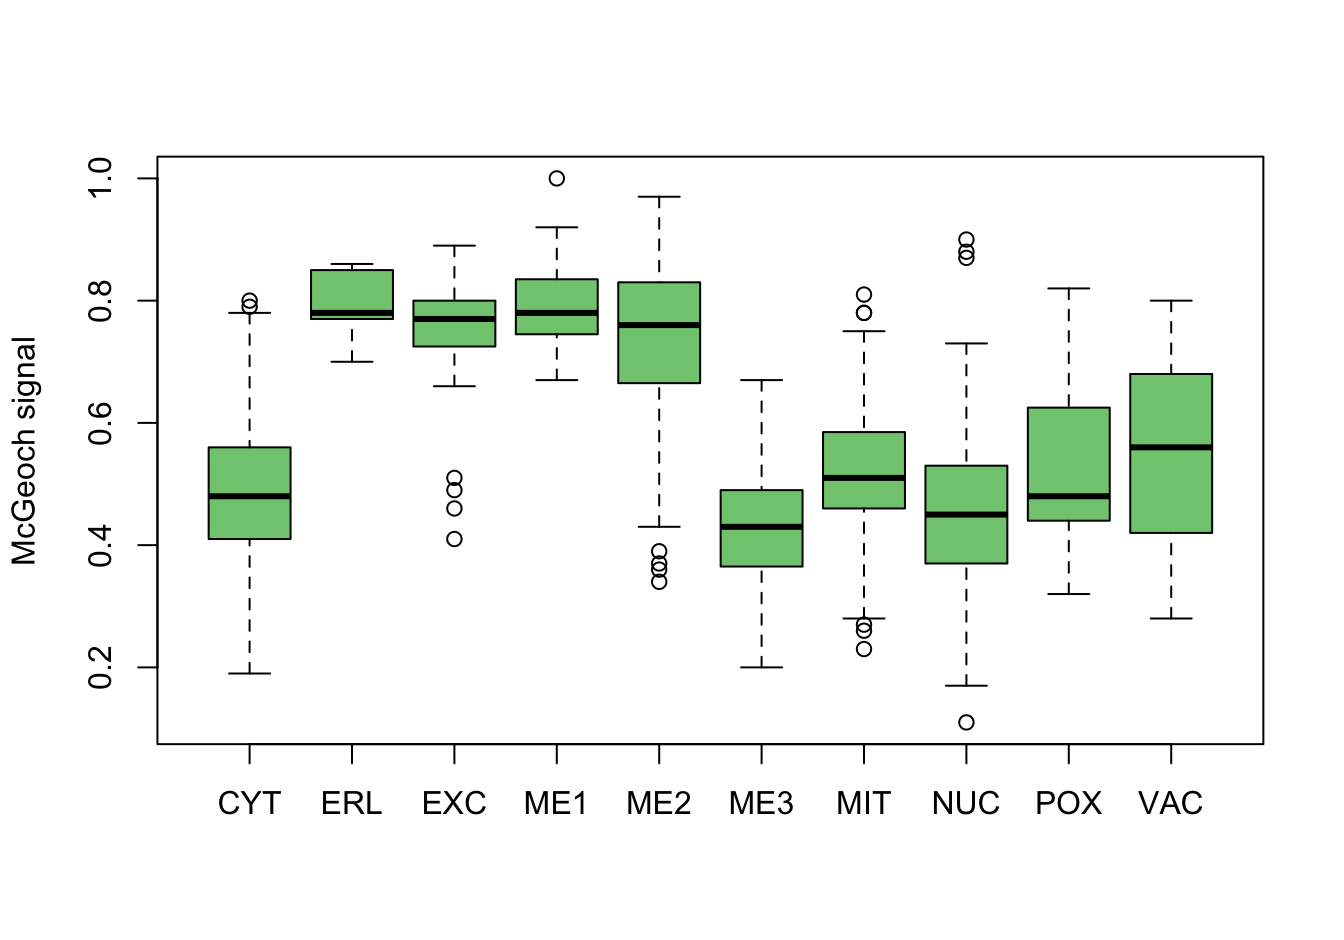
\includegraphics[width=0.7\linewidth]{davur_ebook_files/figure-latex/corr-to-dependent-1} 

}

\caption{Correlations with the dependent variable}\label{fig:corr-to-dependent1}
\end{figure}
\begin{figure}

{\centering 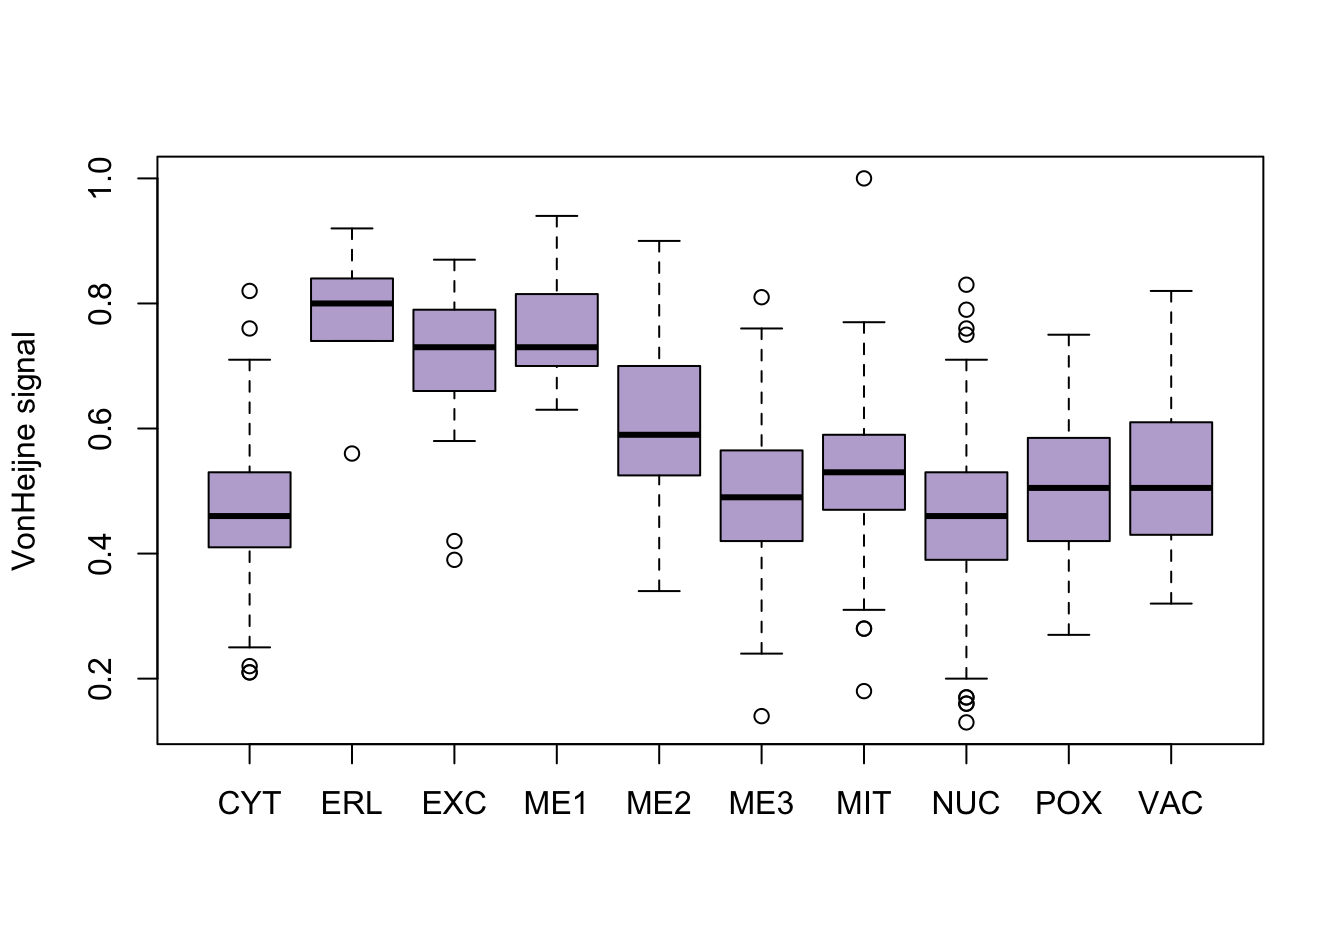
\includegraphics[width=0.7\linewidth]{davur_ebook_files/figure-latex/corr-to-dependent-2} 

}

\caption{Correlations with the dependent variable}\label{fig:corr-to-dependent2}
\end{figure}
\begin{figure}

{\centering 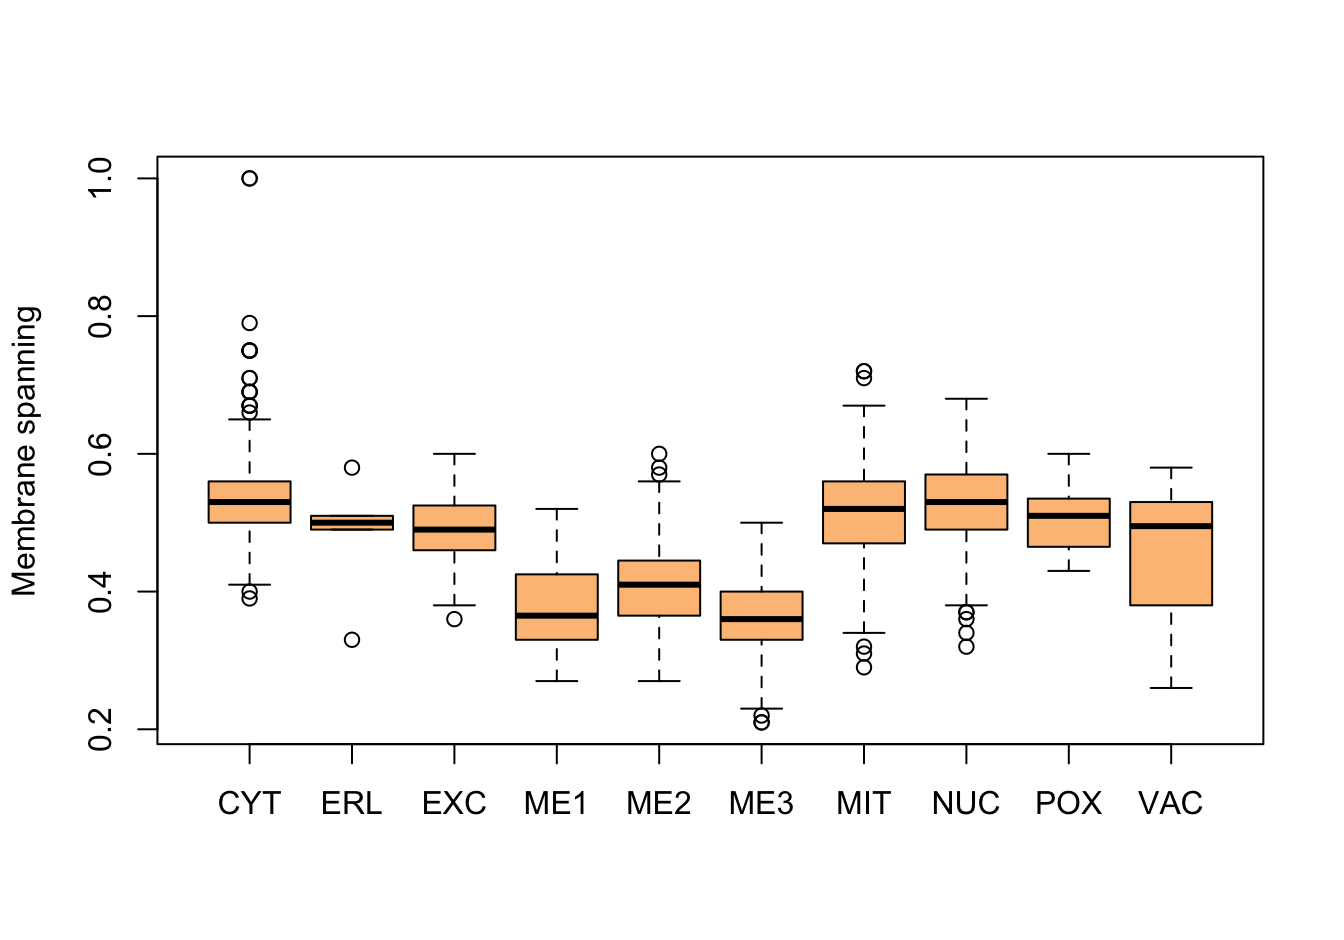
\includegraphics[width=0.7\linewidth]{davur_ebook_files/figure-latex/corr-to-dependent-3} 

}

\caption{Correlations with the dependent variable}\label{fig:corr-to-dependent3}
\end{figure}
\begin{figure}

{\centering 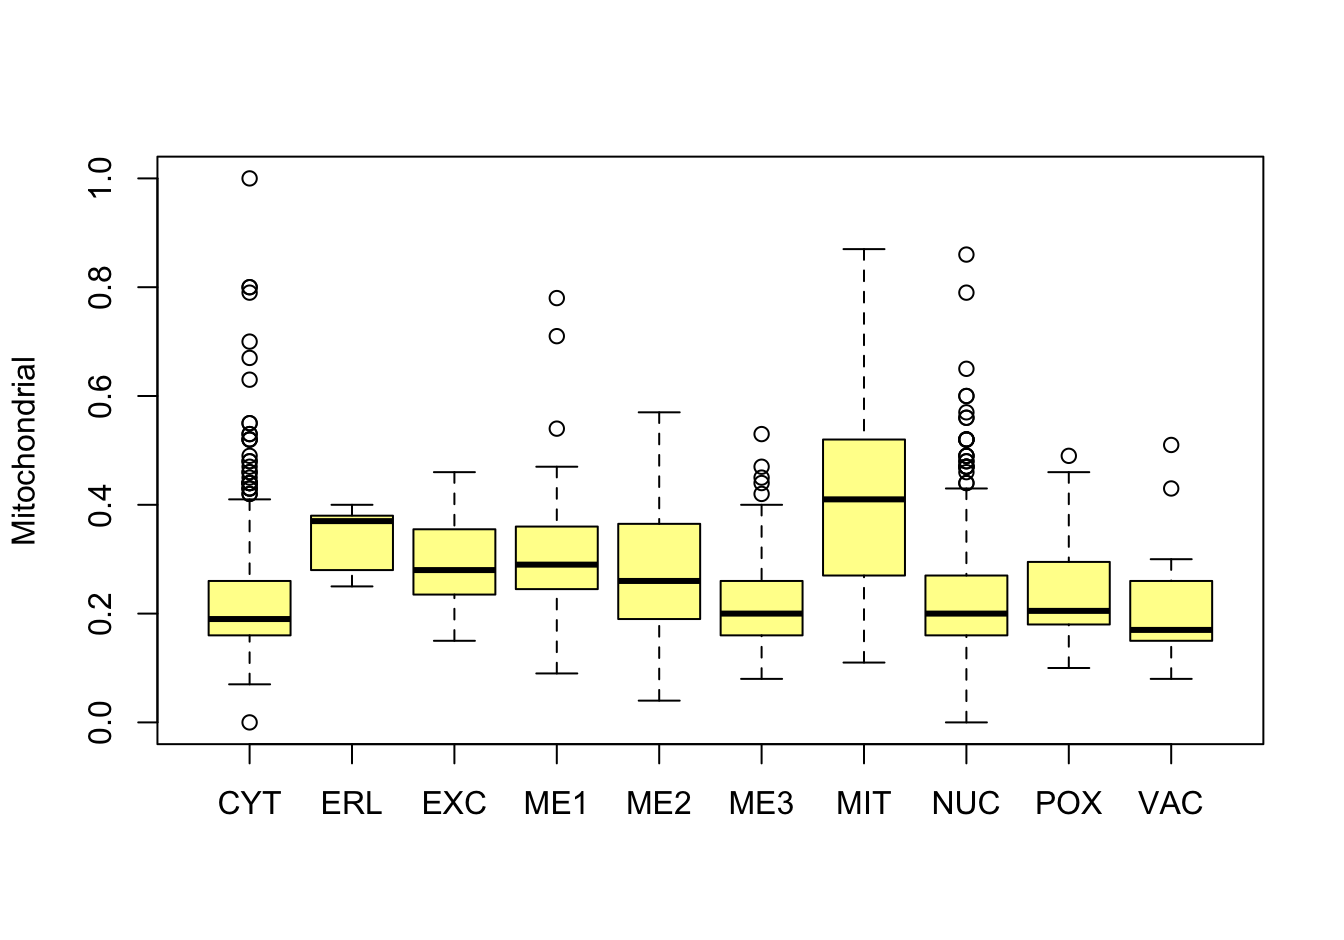
\includegraphics[width=0.7\linewidth]{davur_ebook_files/figure-latex/corr-to-dependent-4} 

}

\caption{Correlations with the dependent variable}\label{fig:corr-to-dependent4}
\end{figure}
\begin{figure}

{\centering 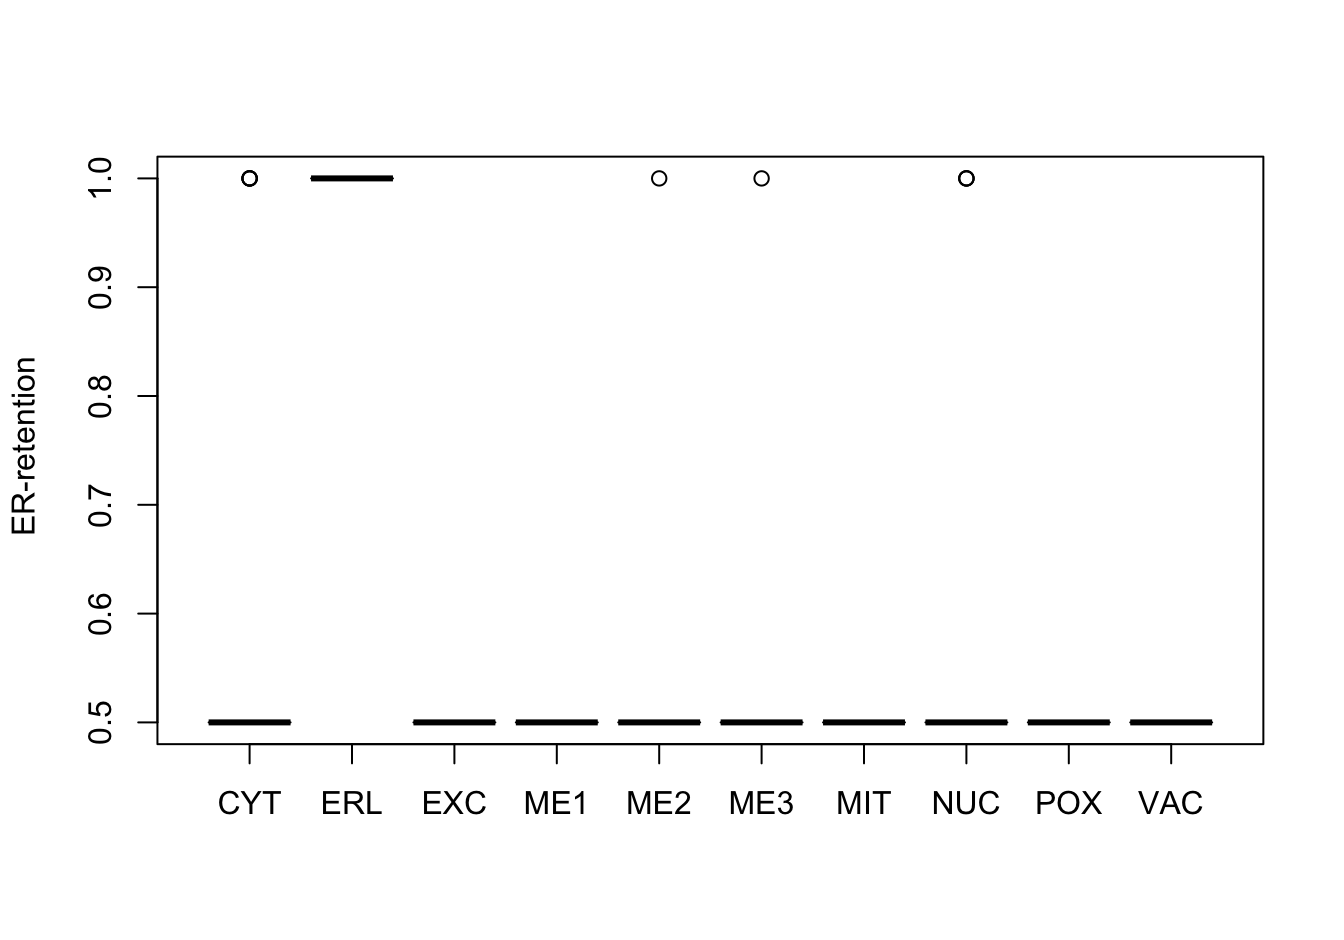
\includegraphics[width=0.7\linewidth]{davur_ebook_files/figure-latex/corr-to-dependent-5} 

}

\caption{Correlations with the dependent variable}\label{fig:corr-to-dependent5}
\end{figure}
\begin{figure}

{\centering 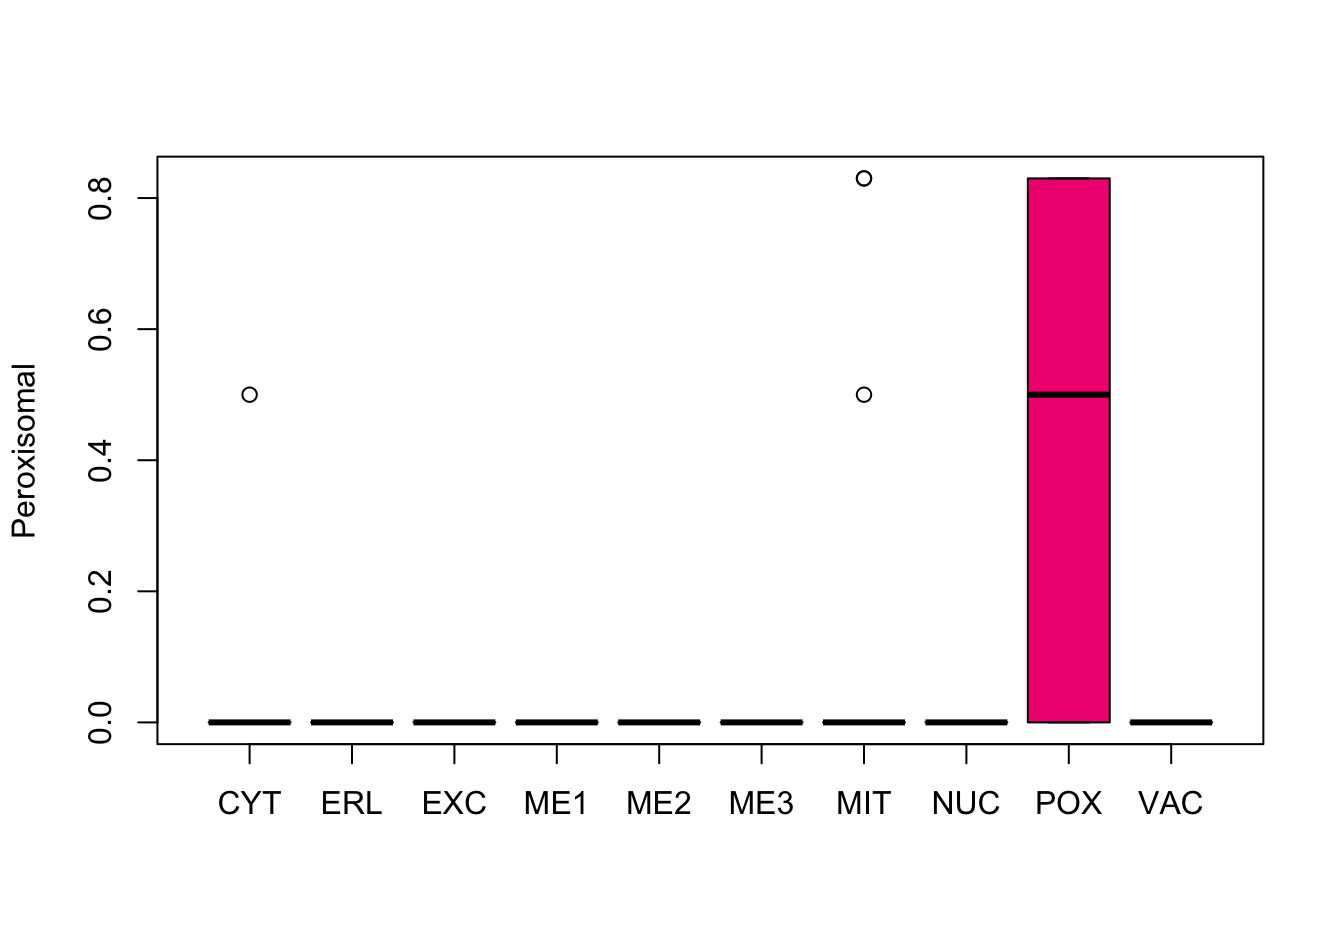
\includegraphics[width=0.7\linewidth]{davur_ebook_files/figure-latex/corr-to-dependent-6} 

}

\caption{Correlations with the dependent variable}\label{fig:corr-to-dependent6}
\end{figure}
\begin{figure}

{\centering 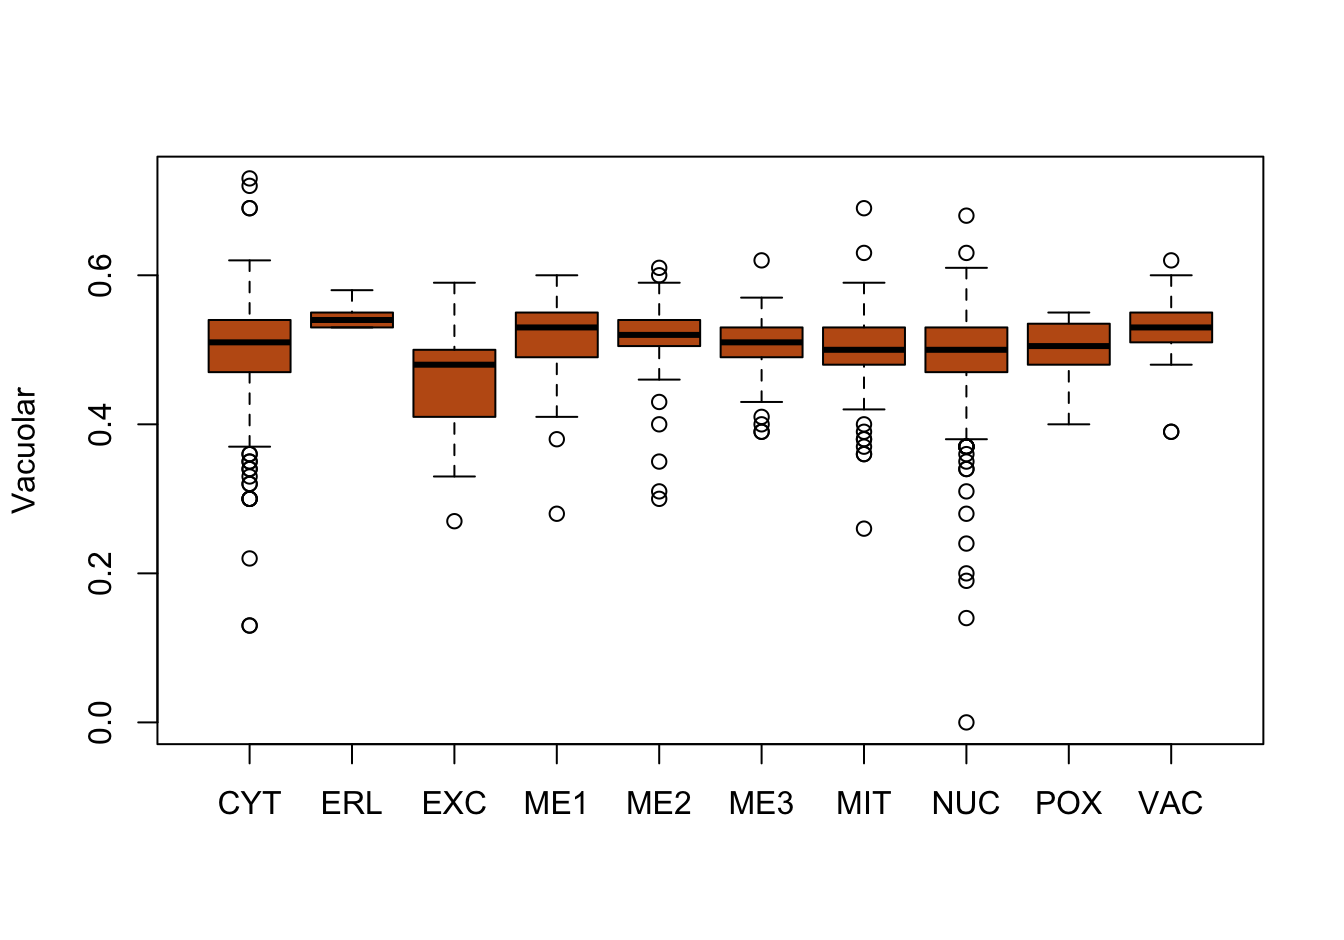
\includegraphics[width=0.7\linewidth]{davur_ebook_files/figure-latex/corr-to-dependent-7} 

}

\caption{Correlations with the dependent variable}\label{fig:corr-to-dependent7}
\end{figure}
\begin{figure}

{\centering \includegraphics[width=0.7\linewidth]{davur_ebook_files/figure-latex/corr-to-dependent-8} 

}

\caption{Correlations with the dependent variable}\label{fig:corr-to-dependent8}
\end{figure}

Quite a few of the variables correlate pretty well with the dependent variable. These do so very well: \texttt{alm}, \texttt{mit}, \texttt{erl}, \texttt{pox}. Others are not: \texttt{nuc}, \texttt{vac}, and some are ambiguous - they discriminate, but not exclusively: \texttt{mcg}, \texttt{gvh}.

Here are some summary statistics for the numeric variables split on the dependent variable:

\begin{Shaded}
\begin{Highlighting}[]
\KeywordTok{options}\NormalTok{(}\DataTypeTok{digits=}\DecValTok{2}\NormalTok{)}

\NormalTok{tmp <-}\StringTok{ }\KeywordTok{t}\NormalTok{(}\KeywordTok{aggregate}\NormalTok{( . }\OperatorTok{~}\StringTok{ }\NormalTok{loc, }\DataTypeTok{data =}\NormalTok{ yeast_data[, }\DecValTok{-1}\NormalTok{], }\DataTypeTok{FUN =}\NormalTok{ mean))}
\NormalTok{knitr}\OperatorTok{::}\KeywordTok{kable}\NormalTok{(tmp)}
\end{Highlighting}
\end{Shaded}

\begin{tabular}{l|l|l|l|l|l|l|l|l|l|l}
\hline
loc & CYT & ERL & EXC & ME1 & ME2 & ME3 & MIT & NUC & POX & VAC\\
\hline
mcg & 0.48 & 0.79 & 0.74 & 0.79 & 0.72 & 0.43 & 0.52 & 0.45 & 0.52 & 0.55\\
\hline
gvh & 0.47 & 0.77 & 0.72 & 0.76 & 0.60 & 0.49 & 0.53 & 0.46 & 0.51 & 0.53\\
\hline
alm & 0.54 & 0.48 & 0.49 & 0.38 & 0.41 & 0.36 & 0.52 & 0.53 & 0.51 & 0.47\\
\hline
mit & 0.23 & 0.34 & 0.29 & 0.31 & 0.28 & 0.21 & 0.40 & 0.23 & 0.25 & 0.20\\
\hline
erl & 0.50 & 1.00 & 0.50 & 0.50 & 0.51 & 0.50 & 0.50 & 0.50 & 0.50 & 0.50\\
\hline
pox & 0.0011 & 0.0000 & 0.0000 & 0.0000 & 0.0000 & 0.0000 & 0.0089 & 0.0000 & 0.4235 & 0.0000\\
\hline
vac & 0.50 & 0.55 & 0.46 & 0.51 & 0.51 & 0.51 & 0.50 & 0.49 & 0.50 & 0.53\\
\hline
nuc & 0.26 & 0.25 & 0.23 & 0.27 & 0.25 & 0.27 & 0.24 & 0.33 & 0.23 & 0.25\\
\hline
\end{tabular}

\begin{Shaded}
\begin{Highlighting}[]
\NormalTok{tmp <-}\StringTok{ }\KeywordTok{t}\NormalTok{(}\KeywordTok{aggregate}\NormalTok{( . }\OperatorTok{~}\StringTok{ }\NormalTok{loc, }\DataTypeTok{data =}\NormalTok{ yeast_data[, }\DecValTok{-1}\NormalTok{], }\DataTypeTok{FUN =}\NormalTok{ median))}
\NormalTok{knitr}\OperatorTok{::}\KeywordTok{kable}\NormalTok{(tmp)}
\end{Highlighting}
\end{Shaded}

\begin{tabular}{l|l|l|l|l|l|l|l|l|l|l}
\hline
loc & CYT & ERL & EXC & ME1 & ME2 & ME3 & MIT & NUC & POX & VAC\\
\hline
mcg & 0.48 & 0.78 & 0.77 & 0.78 & 0.76 & 0.43 & 0.51 & 0.45 & 0.48 & 0.56\\
\hline
gvh & 0.46 & 0.80 & 0.73 & 0.73 & 0.59 & 0.49 & 0.53 & 0.46 & 0.51 & 0.51\\
\hline
alm & 0.53 & 0.50 & 0.49 & 0.36 & 0.41 & 0.36 & 0.52 & 0.53 & 0.51 & 0.49\\
\hline
mit & 0.19 & 0.37 & 0.28 & 0.29 & 0.26 & 0.20 & 0.41 & 0.20 & 0.21 & 0.17\\
\hline
erl & 0.5 & 1.0 & 0.5 & 0.5 & 0.5 & 0.5 & 0.5 & 0.5 & 0.5 & 0.5\\
\hline
pox & 0.0 & 0.0 & 0.0 & 0.0 & 0.0 & 0.0 & 0.0 & 0.0 & 0.5 & 0.0\\
\hline
vac & 0.51 & 0.54 & 0.48 & 0.53 & 0.52 & 0.51 & 0.50 & 0.50 & 0.51 & 0.53\\
\hline
nuc & 0.22 & 0.22 & 0.22 & 0.22 & 0.22 & 0.22 & 0.22 & 0.28 & 0.22 & 0.22\\
\hline
\end{tabular}

\hypertarget{exercises}{%
\chapter{Exercises}\label{exercises}}

This chapter only contains exercises. The solutions are in the next chapter which has a numbering parallel to this one. To work on the exercises it is probably best to create either an RMarkdown Notebook (File → New File → R Notebook) or an RMarkdown document (File → New File → R Markdown\ldots{} → choose Document as type and give it a title). A Notebook has the advantage that you can toggle the visibility of the code, but it has fewer output options (no pdf or Word). I strongly suggest you play around with both.

This is a link to an \href{figures/R_cheatsheet.pdf}{R cheat sheet} that you could use for selecting the right function for a task.

\hypertarget{plotting-rules}{%
\subsubsection*{Plotting rules}\label{plotting-rules}}
\addcontentsline{toc}{subsubsection}{Plotting rules}

With all plots, take care to adhere to the rules regarding titles and other decorations. Tip: the site \href{http://www.statmethods.net/}{Quick-R} has nice detailed information with examples on the different plot types and their configuration. Especially the section \href{http://www.statmethods.net/graphs/index.html}{on plotting} is helpful for these assignments.

\hypertarget{toolbox-1}{%
\section{Toolbox}\label{toolbox-1}}

\hypertarget{get-set-up}{%
\subsection{Get set up}\label{get-set-up}}

Install these tools on your own PC or laptop, in this order:

\begin{enumerate}
\def\labelenumi{\arabic{enumi}.}
\tightlist
\item
  R itself \url{https://cran.r-project.org/bin/windows/base/}\\
\item
  RStudio \url{https://rstudio.com/products/rstudio/download/} (choose the free version of course)
\item
  {[}Optionally{]} If you want to generate pdf documents you should also install a Latex version: MikTeX or TinyTex for Windows or MacTeX on MacOS. If you want to keep things simple I suggest you stick to HTML and MS Word output (Word can also export to PDF).
\end{enumerate}

\hypertarget{resume}{%
\subsection{Résumé}\label{resume}}

Create an R Markdown document called Résumé.Rmd and create your Curriculum Vitae using Markdown syntax. Use the R Markdown Reference Guide or Cheat Sheet or this \href{https://guides.github.com/pdfs/markdown-cheatsheet-online.pdf}{Markdown Cheatsheet} (you don't need R for your résumé so markdown alone is enough).

\hypertarget{basic-r}{%
\section{Basic R}\label{basic-r}}

\hypertarget{math-in-the-console}{%
\subsection{Math in the console}\label{math-in-the-console}}

In the console, calculate the following:

\(31 + 11\)

\(66 - 24\)

\(\frac{126}{3}\)

\(12^2\)

\(\sqrt{256}\)

\(\frac{3*(4+\sqrt{8})}{5^3}\)

\hypertarget{first-look-at-functions}{%
\subsection{First look at functions}\label{first-look-at-functions}}

\textbf{A}\\
View the help page for \texttt{paste()}. There are two variants of this function. Which? And what is the difference between them? Use both variants to generate \emph{exactly} this message \texttt{"welcome\ to\ R"} from these arguments: \texttt{"welcome\ ",\ "to\ ",\ "R"}

\textbf{B}\\
What does the \texttt{abs} function do? What is returned by \texttt{abs(-20)} and what is \texttt{abs(20)}?

\textbf{C}\\
What does the \texttt{c} function do? What is the difference in returned value (result) of \texttt{c()} when you combine either \texttt{1}, \texttt{3} and \texttt{"a"} as arguments, or \texttt{1}, \texttt{2} and \texttt{3}? Use the function \texttt{class()} to answer this.

\textbf{D}\\
What does the function \texttt{install.packages()} do? Use it to install the package \texttt{RColorBrewer}. We'll have a look at this package later on.

\hypertarget{variables-1}{%
\subsection{Variables}\label{variables-1}}

Create three variables with the given values - x=20, y=10 and z=3. Next, calculate the following with these variables:

\begin{enumerate}
\def\labelenumi{\arabic{enumi}.}
\tightlist
\item
  \(x+y\)
\item
  \(x^z\)
\item
  \(q = x \times y \times z\)
\item
  \(\sqrt{q}\)
\item
  \(\frac{q}{\pi}\) (pi is simply pi in R)
\item
  \(\log_{10}{(x \times y)}\)
\end{enumerate}

\hypertarget{vectors-1}{%
\subsection{Vectors}\label{vectors-1}}

\hypertarget{circles}{%
\subsubsection*{Circles}\label{circles}}
\addcontentsline{toc}{subsubsection}{Circles}

The circumference of a circle is \(2\pi\cdot r\), its surface \(4\pi \cdot r^2\) and its volume \(4/3 \pi\cdot r^3\).
Given this vector of circle radiuses,

\begin{Shaded}
\begin{Highlighting}[]
\NormalTok{radiuses <-}\StringTok{ }\KeywordTok{c}\NormalTok{(}\DecValTok{0}\NormalTok{, }\DecValTok{1}\NormalTok{, }\DecValTok{2}\NormalTok{, pi, }\DecValTok{4}\NormalTok{)}
\end{Highlighting}
\end{Shaded}

\textbf{A}\\
Calculate their cirumference.

\textbf{B}\\
Calculate their surface.

\textbf{C}\\
Calculate their volume.

\hypertarget{creating-vectors-1}{%
\subsubsection*{Creating vectors}\label{creating-vectors-1}}
\addcontentsline{toc}{subsubsection}{Creating vectors}

Create the following vectors, \emph{as efficiently as possible}. The functions \texttt{rep()}, \texttt{seq()}, \texttt{paste0()} and the colon operator \texttt{:} can be used, in any combination.

\textbf{A}\\
\texttt{{[}1{]}\ 1\ 2\ 5\ 1\ 2\ 5}

\textbf{B}\\
\texttt{{[}1{]}\ 9\ 9\ 9\ 8\ 8\ 8\ 7\ 7\ 7\ 6\ 6\ 6\ 5\ 5\ 5}

\textbf{C}\\
\texttt{{[}1{]}\ 1\ 1\ 1\ 4\ 4\ 4\ 9\ 9\ 9\ 1\ 1\ 1\ 4\ 4\ 4\ 9\ 9\ 9}

\textbf{D}\\
\texttt{{[}1{]}\ "1a"\ "2b"\ "3c"\ "4d"\ "5e"\ "1a"\ "2b"\ "3c"\ "4d"\ "5e"}

\textbf{E}\\
\texttt{{[}1{]}\ "0z"\ \ \ "0.2y"\ "0.4x"\ "0.6w"\ "0.8v"\ "1u"}

\textbf{F}\\
\texttt{{[}1{]}\ "505"\ "404"\ "303"\ "202"\ "101"\ "000"}

\textbf{G {[}Challenge{]}}\\
\texttt{{[}1{]}\ "0.5A5.0"\ "0.4B4.0"\ "0.3C3.0"\ "0.2D2.0"\ "0.1E1.0"}

\hypertarget{stair-walking-and-heart-rate}{%
\subsection{Stair walking and heart rate}\label{stair-walking-and-heart-rate}}

The vectors below hold data for a staircase walking experiment. A subject of normal weight and height was asked to ascend a (long) stairs wearing a heart-rate monitor. The subjects' heart was registered for different step heights. Create a \textbf{line plot} showing the dependence of heart rate (y axis) on stair height (x axis).

\begin{Shaded}
\begin{Highlighting}[]
\CommentTok{#number of steps on the stairs}
\NormalTok{stair_height <-}\StringTok{ }\KeywordTok{c}\NormalTok{(}\DecValTok{0}\NormalTok{, }\DecValTok{5}\NormalTok{, }\DecValTok{10}\NormalTok{, }\DecValTok{15}\NormalTok{, }\DecValTok{20}\NormalTok{, }\DecValTok{25}\NormalTok{, }\DecValTok{30}\NormalTok{, }\DecValTok{35}\NormalTok{)}
\CommentTok{#heart rate after ascending the stairs}
\NormalTok{heart_rate <-}\StringTok{ }\KeywordTok{c}\NormalTok{(}\DecValTok{66}\NormalTok{, }\DecValTok{65}\NormalTok{, }\DecValTok{67}\NormalTok{, }\DecValTok{69}\NormalTok{, }\DecValTok{73}\NormalTok{, }\DecValTok{79}\NormalTok{, }\DecValTok{86}\NormalTok{, }\DecValTok{97}\NormalTok{)}
\end{Highlighting}
\end{Shaded}

\hypertarget{more-subjects}{%
\subsection{More subjects}\label{more-subjects}}

The experiment from the previous question was extended with three more subjects. One of these subjects was like the first of normal weight, whereas the two others were obese. The data are given below. Create a single \textbf{scatter plot} with connector lines between the points showing the data for all four subjects. Give the normal-weighted subjects a green line and symbol and the obese subjects a red line and symbol.\\
You can add new data series to a plot by using the \texttt{points(x,\ y)} function. Use the \texttt{ylim()} function to adjust the Y-axis range.

\begin{Shaded}
\begin{Highlighting}[]
\CommentTok{#number of steps on the stairs}
\NormalTok{stair_height <-}\StringTok{ }\KeywordTok{c}\NormalTok{(}\DecValTok{0}\NormalTok{, }\DecValTok{5}\NormalTok{, }\DecValTok{10}\NormalTok{, }\DecValTok{15}\NormalTok{, }\DecValTok{20}\NormalTok{, }\DecValTok{25}\NormalTok{, }\DecValTok{30}\NormalTok{, }\DecValTok{35}\NormalTok{)}
\CommentTok{#heart rates for subjects with normal weight}
\NormalTok{heart_rate_}\DecValTok{1}\NormalTok{ <-}\StringTok{ }\KeywordTok{c}\NormalTok{(}\DecValTok{66}\NormalTok{, }\DecValTok{65}\NormalTok{, }\DecValTok{67}\NormalTok{, }\DecValTok{69}\NormalTok{, }\DecValTok{73}\NormalTok{, }\DecValTok{79}\NormalTok{, }\DecValTok{86}\NormalTok{, }\DecValTok{97}\NormalTok{)}
\NormalTok{heart_rate_}\DecValTok{2}\NormalTok{ <-}\StringTok{ }\KeywordTok{c}\NormalTok{(}\DecValTok{61}\NormalTok{, }\DecValTok{61}\NormalTok{, }\DecValTok{63}\NormalTok{, }\DecValTok{68}\NormalTok{, }\DecValTok{74}\NormalTok{, }\DecValTok{81}\NormalTok{, }\DecValTok{89}\NormalTok{, }\DecValTok{104}\NormalTok{)}
\CommentTok{#heart rates for obese subjects}
\NormalTok{heart_rate_}\DecValTok{3}\NormalTok{ <-}\StringTok{ }\KeywordTok{c}\NormalTok{(}\DecValTok{58}\NormalTok{, }\DecValTok{60}\NormalTok{, }\DecValTok{67}\NormalTok{, }\DecValTok{71}\NormalTok{, }\DecValTok{78}\NormalTok{, }\DecValTok{89}\NormalTok{, }\DecValTok{104}\NormalTok{, }\DecValTok{121}\NormalTok{)}
\NormalTok{heart_rate_}\DecValTok{4}\NormalTok{ <-}\StringTok{ }\KeywordTok{c}\NormalTok{(}\DecValTok{69}\NormalTok{, }\DecValTok{73}\NormalTok{, }\DecValTok{77}\NormalTok{, }\DecValTok{83}\NormalTok{, }\DecValTok{88}\NormalTok{, }\DecValTok{96}\NormalTok{, }\DecValTok{102}\NormalTok{, }\DecValTok{127}\NormalTok{)}
\end{Highlighting}
\end{Shaded}

\hypertarget{chickens-on-a-diet}{%
\subsection{Chickens on a diet}\label{chickens-on-a-diet}}

The body weights of chicks were measured at birth and every second day thereafter until day 20. They were also measured on day 21. In the experiment there were four groups of chicks on different protein diets. Here are the data for the first four chicks. Chick one and two were on diet 1 and chick three and four were on diet 2. Create a single line plot showing the data for all four chicks. Give each chick its own color.

\begin{Shaded}
\begin{Highlighting}[]
\CommentTok{# chick weight data}
\NormalTok{time <-}\StringTok{ }\KeywordTok{c}\NormalTok{(}\DecValTok{0}\NormalTok{, }\DecValTok{2}\NormalTok{, }\DecValTok{4}\NormalTok{, }\DecValTok{6}\NormalTok{, }\DecValTok{8}\NormalTok{, }\DecValTok{10}\NormalTok{, }\DecValTok{12}\NormalTok{, }\DecValTok{14}\NormalTok{, }\DecValTok{16}\NormalTok{, }\DecValTok{18}\NormalTok{, }\DecValTok{20}\NormalTok{, }\DecValTok{21}\NormalTok{)}
\NormalTok{chick_}\DecValTok{1}\NormalTok{ <-}\StringTok{ }\KeywordTok{c}\NormalTok{(}\DecValTok{42}\NormalTok{, }\DecValTok{51}\NormalTok{, }\DecValTok{59}\NormalTok{, }\DecValTok{64}\NormalTok{, }\DecValTok{76}\NormalTok{, }\DecValTok{93}\NormalTok{, }\DecValTok{106}\NormalTok{, }\DecValTok{125}\NormalTok{, }\DecValTok{149}\NormalTok{, }\DecValTok{171}\NormalTok{, }\DecValTok{199}\NormalTok{, }\DecValTok{205}\NormalTok{)}
\NormalTok{chick_}\DecValTok{2}\NormalTok{ <-}\StringTok{ }\KeywordTok{c}\NormalTok{(}\DecValTok{40}\NormalTok{, }\DecValTok{49}\NormalTok{, }\DecValTok{58}\NormalTok{, }\DecValTok{72}\NormalTok{, }\DecValTok{84}\NormalTok{, }\DecValTok{103}\NormalTok{, }\DecValTok{122}\NormalTok{, }\DecValTok{138}\NormalTok{, }\DecValTok{162}\NormalTok{, }\DecValTok{187}\NormalTok{, }\DecValTok{209}\NormalTok{, }\DecValTok{215}\NormalTok{)}
\NormalTok{chick_}\DecValTok{3}\NormalTok{ <-}\StringTok{ }\KeywordTok{c}\NormalTok{(}\DecValTok{42}\NormalTok{, }\DecValTok{53}\NormalTok{, }\DecValTok{62}\NormalTok{, }\DecValTok{73}\NormalTok{, }\DecValTok{85}\NormalTok{, }\DecValTok{102}\NormalTok{, }\DecValTok{123}\NormalTok{, }\DecValTok{138}\NormalTok{, }\DecValTok{170}\NormalTok{, }\DecValTok{204}\NormalTok{, }\DecValTok{235}\NormalTok{, }\DecValTok{256}\NormalTok{)}
\NormalTok{chick_}\DecValTok{4}\NormalTok{ <-}\StringTok{ }\KeywordTok{c}\NormalTok{(}\DecValTok{41}\NormalTok{, }\DecValTok{49}\NormalTok{, }\DecValTok{61}\NormalTok{, }\DecValTok{74}\NormalTok{, }\DecValTok{98}\NormalTok{, }\DecValTok{109}\NormalTok{, }\DecValTok{128}\NormalTok{, }\DecValTok{154}\NormalTok{, }\DecValTok{192}\NormalTok{, }\DecValTok{232}\NormalTok{, }\DecValTok{280}\NormalTok{, }\DecValTok{290}\NormalTok{)}
\end{Highlighting}
\end{Shaded}

\hypertarget{chicken-bar-plot}{%
\subsection{Chicken bar plot}\label{chicken-bar-plot}}

With the data from the previous question, create a bar plot of the maximum weights of the chicks.

\hypertarget{discoveries}{%
\subsection{Discoveries}\label{discoveries}}

The R language comes with a wealth of datasets for you to use as practice materials. We will see several of these. One of these datasets is The Time-Series dataset called \texttt{discoveries} holding the numbers of ``great'' inventions and scientific discoveries in each year from 1860 to 1959. Type its name in the console to see it. Create plot(s) answering these questions:

\textbf{A}\\
What is the number of discoveries per year? Use the \texttt{barplot()} and \texttt{table()} functions for this.

\textbf{B}\\
What is the 5-number summary of discoveries per year?

\textbf{C}\\
What is the trend over time for the numbers of discoveries per year?

PS: This is actually not a simple vector but a vector with some time-related attributes. It is called a Time-Series (a \texttt{ts} class), but this does not really matter for this assignment.

\hypertarget{lung-cancer}{%
\subsection{Lung cancer}\label{lung-cancer}}

The R datasets package has three related timeseries datasets relating to lung cancer deaths. These are \texttt{ldeaths}, \texttt{mdeaths} and \texttt{fdeaths} for total, male and female deaths respectively. Create a line plot showing the monthly mortality holding all three of these datasets. Use the \texttt{legend()} function to add a legend to the plot, as demonstrated in this example:

\begin{Shaded}
\begin{Highlighting}[]
\NormalTok{t <-}\StringTok{ }\DecValTok{1}\OperatorTok{:}\DecValTok{5}
\NormalTok{y1 <-}\StringTok{ }\KeywordTok{c}\NormalTok{(}\DecValTok{2}\NormalTok{, }\DecValTok{3}\NormalTok{, }\DecValTok{5}\NormalTok{, }\DecValTok{4}\NormalTok{, }\DecValTok{6}\NormalTok{)}
\NormalTok{y2 <-}\StringTok{ }\KeywordTok{c}\NormalTok{(}\DecValTok{1}\NormalTok{, }\DecValTok{3}\NormalTok{, }\DecValTok{4}\NormalTok{, }\DecValTok{5}\NormalTok{, }\DecValTok{7}\NormalTok{)}
\KeywordTok{plot}\NormalTok{(t, y1, }\DataTypeTok{type =} \StringTok{"b"}\NormalTok{, }\DataTypeTok{ylab =} \StringTok{"response"}\NormalTok{, }\DataTypeTok{ylim =} \KeywordTok{c}\NormalTok{(}\DecValTok{0}\NormalTok{, }\DecValTok{8}\NormalTok{))}
\KeywordTok{points}\NormalTok{(t, y2, }\DataTypeTok{col =} \StringTok{"blue"}\NormalTok{, }\DataTypeTok{type =} \StringTok{"b"}\NormalTok{)}
\KeywordTok{legend}\NormalTok{(}\StringTok{"topleft"}\NormalTok{, }\DataTypeTok{legend =} \KeywordTok{c}\NormalTok{(}\StringTok{"series 1"}\NormalTok{, }\StringTok{"series 2"}\NormalTok{), }\DataTypeTok{col =} \KeywordTok{c}\NormalTok{(}\StringTok{"black"}\NormalTok{, }\StringTok{"blue"}\NormalTok{), }\DataTypeTok{pch =} \DecValTok{1}\NormalTok{, }\DataTypeTok{lty =} \DecValTok{1}\NormalTok{)}
\end{Highlighting}
\end{Shaded}

\begin{center}\includegraphics[width=0.8\linewidth]{davur_ebook_files/figure-latex/legend-demo-1} \end{center}

\textbf{A}\\
Create the mentioned line plot. Do you see trends and/or patterns and if so, can you explain these?

\textbf{B}\\
Create a combined boxplot of the three time-series. Are there outliers? If so, can you figure out when this occurred, and why?

\hypertarget{complex-datatypes}{%
\section{Complex datatypes}\label{complex-datatypes}}

This section serves you some datatype challenges.

\hypertarget{creating-factors}{%
\subsection{Creating factors}\label{creating-factors}}

\textbf{A}\\
Given this vector:

\begin{Shaded}
\begin{Highlighting}[]
\NormalTok{animal_risk <-}\StringTok{ }\KeywordTok{c}\NormalTok{(}\DecValTok{2}\NormalTok{, }\DecValTok{4}\NormalTok{, }\DecValTok{1}\NormalTok{, }\DecValTok{1}\NormalTok{, }\DecValTok{2}\NormalTok{, }\DecValTok{4}\NormalTok{, }\DecValTok{1}\NormalTok{, }\DecValTok{4}\NormalTok{, }\DecValTok{1}\NormalTok{, }\DecValTok{1}\NormalTok{, }\DecValTok{2}\NormalTok{, }\DecValTok{1}\NormalTok{)}
\end{Highlighting}
\end{Shaded}

and these possible levels:
1: harmless
2: risky
3: dangerous
4: deadly

Create a factor from this data and then barplot the result.

\textbf{B}\\
Given this data, a simulation of wealth distribution of ``poor'', ``middle class'', ``wealthy'' "rich:

\begin{Shaded}
\begin{Highlighting}[]
\KeywordTok{set.seed}\NormalTok{(}\DecValTok{1234}\NormalTok{)}
\NormalTok{wealth_male <-}\StringTok{ }\KeywordTok{sample}\NormalTok{(}\DataTypeTok{x =}\NormalTok{ letters[}\DecValTok{1}\OperatorTok{:}\DecValTok{4}\NormalTok{], }
                 \DataTypeTok{size =} \DecValTok{1000}\NormalTok{,}
                 \DataTypeTok{replace=} \OtherTok{TRUE}\NormalTok{, }
                 \DataTypeTok{prob =} \KeywordTok{c}\NormalTok{(}\FloatTok{0.7}\NormalTok{, }\FloatTok{0.17}\NormalTok{, }\FloatTok{0.12}\NormalTok{, }\FloatTok{0.01}\NormalTok{))}
\NormalTok{wealth_female <-}\StringTok{ }\KeywordTok{sample}\NormalTok{(}\DataTypeTok{x =}\NormalTok{ letters[}\DecValTok{1}\OperatorTok{:}\DecValTok{4}\NormalTok{], }
                 \DataTypeTok{size =} \DecValTok{1000}\NormalTok{,}
                 \DataTypeTok{replace=} \OtherTok{TRUE}\NormalTok{, }
                 \DataTypeTok{prob =} \KeywordTok{c}\NormalTok{(}\FloatTok{0.8}\NormalTok{, }\FloatTok{0.15}\NormalTok{, }\FloatTok{0.497}\NormalTok{, }\FloatTok{0.003}\NormalTok{))}
\end{Highlighting}
\end{Shaded}

Create a factor from these two and report the cumulative percentage of its individual levels starting at the most abundant level, combined for male and female. Hint: use \texttt{table()} and \texttt{prop.table()}.

Next, create a side-by-side barplot of this data. Don't forget the legend!

\hypertarget{a-dictionary-with-a-named-vector}{%
\subsection{A dictionary with a named vector}\label{a-dictionary-with-a-named-vector}}

Almost all programming languages know the (hash)map / dictionary data structure storing so-called ``key-and-value'' pairs. They make it possible to ``look up'' the value belonging to a ``key''. That is where the term dictionary comes from. A dictionary holds keys (the words) and their meaning (values). R does not have a dictionary type but you could make a dict-like structure using a \textbf{\emph{vector with named elements}}. Here follows an example.

If I wanted to create and use a DNA codon translation table, and use it to translate a piece of DNA, I could do something like what is shown below (there are only 4 of the 64 codons included). See if you can figure out what is going on there

\begin{Shaded}
\begin{Highlighting}[]
\CommentTok{## define codon table as named vector}
\NormalTok{codons <-}\StringTok{ }\KeywordTok{c}\NormalTok{(}\StringTok{"Gly"}\NormalTok{, }\StringTok{"Pro"}\NormalTok{, }\StringTok{"Lys"}\NormalTok{, }\StringTok{"Ser"}\NormalTok{)}
\KeywordTok{names}\NormalTok{(codons) <-}\StringTok{ }\KeywordTok{c}\NormalTok{(}\StringTok{"GGA"}\NormalTok{, }\StringTok{"CCU"}\NormalTok{, }\StringTok{"AAA"}\NormalTok{, }\StringTok{"AGU"}\NormalTok{)}

\CommentTok{## the DNA to translate}
\NormalTok{my_DNA <-}\StringTok{ "GGACCUAAAAGU"}
\NormalTok{my_prot <-}\StringTok{ ""}
\CommentTok{## iterate the DNA and take only every position}
\ControlFlowTok{for}\NormalTok{ (i }\ControlFlowTok{in} \KeywordTok{seq}\NormalTok{(}\DecValTok{1}\NormalTok{, }\KeywordTok{nchar}\NormalTok{(my_DNA), }\DataTypeTok{by=}\DecValTok{3}\NormalTok{)) \{}
\NormalTok{    codon <-}\StringTok{ }\KeywordTok{substr}\NormalTok{(my_DNA, i, i}\OperatorTok{+}\DecValTok{2}\NormalTok{);}
\NormalTok{    my_prot <-}\StringTok{ }\KeywordTok{paste}\NormalTok{(my_prot, codons[codon])}
\NormalTok{\}}
\KeywordTok{print}\NormalTok{(my_prot)}
\end{Highlighting}
\end{Shaded}

\begin{verbatim}
## [1] " Gly Pro Lys Ser"
\end{verbatim}

\textbf{A}\\
Make a modified copy of this code chunk in such a way that no spaces are present between the amino acid residues (use help on \texttt{paste()} to figure this out) and that single-letter codes of amino acids are used instead of three-letter codes.

\textbf{B}\\
\textbf{{[}Challenge{]}} Here is a vector called \texttt{nuc\_weights}. It holds the weights for the nucleotides A, C, G and U respectively. Make it a named vector, iterate \texttt{my\_DNA} from the above code chunk and calculate its molecular weight.

\begin{Shaded}
\begin{Highlighting}[]
\NormalTok{nuc_weights <-}\StringTok{ }\KeywordTok{c}\NormalTok{(}\FloatTok{491.2}\NormalTok{, }\FloatTok{467.2}\NormalTok{, }\FloatTok{507.2}\NormalTok{, }\FloatTok{482.2}\NormalTok{)}
\end{Highlighting}
\end{Shaded}

\hypertarget{airquality}{%
\subsection{airquality}\label{airquality}}

The \texttt{airquality} dataset is also one of the datasets included in the \texttt{datasets} package. We'll explore this for a few questions.

\textbf{A}\\
Create a scatterplot of Temperature as a function of Solar radiation. Is there, as you might naively expect, a strong correlation? You could use \texttt{cor.test()} to find out. Add a linear model using \texttt{lm()} to extend your plot.

\textbf{B}\\
Create a boxplot-series of \texttt{Temp} as a function of \texttt{Month} (use \texttt{?boxplot} to find out how this works). What appears to be the warmest month?

\textbf{C}\\
What date (day/month) has the lowest recorded temperature? Which the highest? Please give temperature values in Celsius, not Fahrenheit! (Yes, this is an extra challenge!)

\textbf{D}\\
Create a histogram of the wind speeds, and add a thick blue vertical line for the value of the mean and a fat red line for the median (use \texttt{abline()} for this).

\textbf{E}\\
Use the \texttt{pairs()} function with argument \texttt{panel\ =\ panel.smooth} to plot all pairwise correlations between Ozone, Solar radiation, Wind and Temperature. Which pair shows the strongest correlation in your opinion? Verify this using the \texttt{cor()} function after removing incomplete cases. Create a separate well annotated scatterplot of this pair.

\hypertarget{bird-observations}{%
\subsection{Bird observations}\label{bird-observations}}

You will explore a bird observation dataset, downloaded from \href{http://goldengateaudubon.org/birding-resources/observations/}{GOLDEN GATE AUDUBON SOCIETY}. This file lists bird observations collected by this bird monitoring group in the San Francisco Bay Area. I already cleaned it a bit and placed it here: \url{data/Observations-Data-2014.csv}.

You can download it as follows:

\begin{Shaded}
\begin{Highlighting}[]
\NormalTok{file_name <-}\StringTok{ "Observations-Data-2014.csv"}
\NormalTok{remote_url <-}\StringTok{ }\KeywordTok{paste0}\NormalTok{(}\StringTok{"https://raw.githubusercontent.com/MichielNoback/davur1_gitbook/master/data/"}\NormalTok{, file_name)}

\KeywordTok{download.file}\NormalTok{(}\DataTypeTok{url =}\NormalTok{ remote_url, }\DataTypeTok{destfile =}\NormalTok{ file_name)}
\end{Highlighting}
\end{Shaded}

Load the observation data into R and assign it to a variable called \texttt{bird\_obs}.

From here on, it is assumed that you have the dataframe \texttt{bird\_obs} loaded. This series of exercises deals with cleaning and transforming data, and exploring a cleaned dataset using basic plotting techniques and descriptive statistics.

\textbf{A}\\
First, explore the raw data as they are.

\begin{itemize}
\tightlist
\item
  What data on bird observations were recorded (i.e.~what kind of variables do you have)?
\item
  What did R do to the original column names?
\item
  Are all column names clear to you?
\end{itemize}

\textbf{B}\\
How many bird observations were recorded?

\textbf{C}\\
The column holding observation ``Number'' is actually not a number. Into what type has R converted it?

\textbf{D}\\
Convert the ``Number'' column into an integer column using \texttt{as.integer()}, but assign it to a new column called ``Count'' (i.e.~do not overwrite the original values). Compare the first 50 values or so of these two columns. What happened to the data? Is this OK?

\textbf{E}\\
The previous question has shown that converting factors to numbers is a bit dangerous. It is often easiest to convert characters to numbers. The best way to do this is by using the \texttt{as.is\ =\ c(\textless{}column\ indices\textgreater{})} argument for the \texttt{read.table()} function.

So, which columns should be loaded as real factor data and which as plain character data? Use \texttt{read.table()} and the \texttt{as.is} argument to reload the data, and then transform the \texttt{Number} column to integer again as \texttt{Count}.

\textbf{F}\\
Compare the first 50 values of the Number and Count columns again. Has the conversion succeeded? How many \texttt{Number} values could not be transformed into an integer value? Hint: use \texttt{is.na()}

\textbf{G}\\
Explore the sighting counts:

\begin{itemize}
\tightlist
\item
  What is the maximum number of birds in a single sighting? (Use max() and which() or is.na() to solve this)
\item
  What is the mean sighting count
\item
  What is the median of the sighting count
\end{itemize}

\textbf{H}\\
Is the \texttt{Count} variable a normal distributed value? You can use \texttt{hist(...)}, \texttt{table()} or \texttt{plot(density(...))} to explore this further.

\textbf{I}\\
Explore the species constitution:

\begin{itemize}
\tightlist
\item
  How many different species were recorded?
\item
  How many genera do they constitute?
\item
  What species from the genus ``Puffinus'' have been observed?
\end{itemize}

Hint: use the function \texttt{unique()} here.

\textbf{J {[}Challenge{]}}\\
This is a challenge exercise for those who like to grind their brains! Think of a strategy to ``rescue'' the NAs that appear after transforming ``Number'' to ``Count''. Hint: use \texttt{gsub()} or\texttt{grep()}

\hypertarget{regular-expressions}{%
\section{Regular Expressions}\label{regular-expressions}}

\hypertarget{restriction-enzymes-1}{%
\subsection{Restriction enzymes}\label{restriction-enzymes-1}}

\textbf{A}\\
The restriction enzyme PacI has the recognition sequence ``TTAATTAA''. Define (at least) three alternative regex patterns that will catch these sites.

\textbf{B}\\
The restriction enzyme SfiI has the recognition sequence ``GGCCNNNNNGGCC''. Define (at least) three alternative regex patterns that will catch these sites.

\hypertarget{prosite-patterns-1}{%
\subsection{Prosite Patterns}\label{prosite-patterns-1}}

\textbf{A}\\
The Prosite pattern PS00211 (ABC-transporter-1; \url{https://prosite.expasy.org/PS00211}) has the pattern:\\
``{[}LIVMFYC{]}-{[}SA{]}-{[}SAPGLVFYKQH{]}-G-{[}DENQMW{]}-{[}KRQASPCLIMFW{]}-{[}KRNQSTAVM{]}-{[}KRACLVM{]}-{[}LIVMFYPAN{]}-\{PHY\}-{[}LIVMFW{]}-{[}SAGCLIVP{]}-\{FYWHP\}-\{KRHP\}-{[}LIVMFYWSTA{]}.''
Translate it into a regex pattern. Info on the syntax is here: \url{https://prosite.expasy.org/prosuser.html\#conv_pa}

\textbf{B}\\
The Prosite pattern PS00018 (EF-hand calcium-binding domain; \url{https://prosite.expasy.org/PS00018}) has the pattern:
``D-\{W\}-{[}DNS{]}-\{ILVFYW\}-{[}DENSTG{]}-{[}DNQGHRK{]}-\{GP\}-{[}LIVMC{]}-{[}DENQSTAGC{]}-x(2)- {[}DE{]}-{[}LIVMFYW{]}.''
Translate it into a regex pattern.

You could exercise more by simply browsing Prosite. Test your pattern by fetching the proteins referred to within the Prosite pattern details page.

\hypertarget{fasta-headers}{%
\subsection{Fasta Headers}\label{fasta-headers}}

The fasta sequence format is a very common sequence file format used in molecular biology.
It looks like this (I omitted most of the actual protein sequences for better representation):

\begin{verbatim}
>gi|21595364|gb|AAH32336.1| FHIT protein [Homo sapiens]
MSFRFGQHLIK...ALRVYFQ
>gi|15215093|gb|AAH12662.1| Fhit protein [Mus musculus]
MSFRFGQHLIK...RVYFQA
>gi|151554847|gb|AAI47994.1| FHIT protein [Bos taurus]
MSFRFGQHLIK...LRVYFQ
\end{verbatim}

As you can see there are several distinct elements within the Fasta \textbf{\emph{header}} which is the description line above the actual sequence: one or more database identification strings, a protein description or name and an organism name. Study the format - we are going to extract some elements from these fasta headers using the \texttt{stringr} package. Install it if you don't have it yet.

Here is a small example:

\begin{Shaded}
\begin{Highlighting}[]
\KeywordTok{library}\NormalTok{(stringr)}
\NormalTok{hinfII_re <-}\StringTok{ "GA[GATC]TC"}
\NormalTok{sequences <-}\StringTok{ }\KeywordTok{c}\NormalTok{(}\StringTok{"GGGAATCC"}\NormalTok{, }\StringTok{"TCGATTCGC"}\NormalTok{, }\StringTok{"ACGAGTCTA"}\NormalTok{)}
\KeywordTok{str_extract}\NormalTok{(}\DataTypeTok{string =}\NormalTok{ sequences,}
            \DataTypeTok{pattern =}\NormalTok{ hinfII_re)}
\end{Highlighting}
\end{Shaded}

\begin{verbatim}
## [1] "GAATC" "GATTC" "GAGTC"
\end{verbatim}

Function \texttt{str\_extract()} simply extracts the exact match of your regex (shown above). On the other hand, function \texttt{str\_match()} supports \textbf{\emph{grouping capture}} through bounding parentheses:

\begin{Shaded}
\begin{Highlighting}[]
\NormalTok{phones <-}\StringTok{ }\KeywordTok{c}\NormalTok{(}\StringTok{"+31-6-23415239"}\NormalTok{, }\StringTok{"+49-51-55523146"}\NormalTok{, }\StringTok{"+31-50-5956566"}\NormalTok{)}
\NormalTok{phones_re <-}\StringTok{ "}\CharTok{\textbackslash{}\textbackslash{}}\StringTok{+(}\CharTok{\textbackslash{}\textbackslash{}}\StringTok{d\{2\})-(}\CharTok{\textbackslash{}\textbackslash{}}\StringTok{d\{1,2\})"} \CommentTok{#matching country codes and area codes}
\NormalTok{matches <-}\StringTok{ }\KeywordTok{str_match}\NormalTok{(phones, phones_re) }
\NormalTok{matches}
\end{Highlighting}
\end{Shaded}

\begin{verbatim}
##      [,1]     [,2] [,3]
## [1,] "+31-6"  "31" "6" 
## [2,] "+49-51" "49" "51"
## [3,] "+31-50" "31" "50"
\end{verbatim}

Thus, each set of parentheses will yield a column in the returned matrix. Simply use its column index to get that result set:

\begin{Shaded}
\begin{Highlighting}[]
\NormalTok{matches[, }\DecValTok{2}\NormalTok{] }\CommentTok{##the country codes}
\end{Highlighting}
\end{Shaded}

\begin{verbatim}
## [1] "31" "49" "31"
\end{verbatim}

Now, given the fasta headers in \url{./data/fasta_headers.txt}
which you can simply load into a character vector using \texttt{readLines()}, extract the following.

\textbf{A}\\
- Extract all complete organism names.\\
- Extract all species-level organism names (omitting subspecies and strains etc).

\textbf{B}\\
Extract all \textbf{\emph{first}} database identifiers. So in this header element \texttt{\textgreater{}gi\textbar{}224017144\textbar{}gb\textbar{}EEF75156.1\textbar{}} you should extract only \texttt{gi\textbar{}224017144}

\textbf{C}\\
Extract all protein names/descriptions.

\hypertarget{scripting-2}{%
\section{Scripting}\label{scripting-2}}

This section serves you some exercises that will help you improve your function-writing skills.

\hypertarget{illegal-reproductions}{%
\subsection{Illegal reproductions}\label{illegal-reproductions}}

As an exercise, you will re-invent the wheel here for some statistical functions.

\hypertarget{the-mean}{%
\subsubsection*{The mean}\label{the-mean}}
\addcontentsline{toc}{subsubsection}{The mean}

Create a function, \texttt{my\_mean()}, that duplicates the R function \texttt{mean()}, i.e.~calculates and returns the mean of a vector of numbers, without actually using \texttt{mean()}.

\hypertarget{standard-deviation}{%
\subsubsection*{Standard deviation}\label{standard-deviation}}
\addcontentsline{toc}{subsubsection}{Standard deviation}

Create a function, \texttt{my\_sd()}, that duplicates the R function \texttt{sd()}, i.e.~calculates and returns the standard deviation of a vector of numbers, without actually using \texttt{sd()}.

\hypertarget{median}{%
\subsubsection*{Median}\label{median}}
\addcontentsline{toc}{subsubsection}{Median}

\textbf{{[}Challenge{]}} Create a function, \texttt{my\_median()}, that duplicates the R function \texttt{median()}, i.e.~calculates and returns the median of a vector of numbers. This is actually a bit harder than you might expect. Hint: use the \texttt{sort()} function.

\hypertarget{interquantile-ranges}{%
\subsection{Interquantile ranges}\label{interquantile-ranges}}

Create a function that will calculate a custom ``interquantile range''. The function should accept three arguments: a numeric vector, a lower quantile and an upper quantile. It should return the difference (range) between these two quantile values. The lower quantile should default to 0 and the higher to 1, thus returning \texttt{max(x)} minus \texttt{min(x)}. The function therefore has this ``signature'':

\begin{Shaded}
\begin{Highlighting}[]
\NormalTok{interquantile_range <-}\StringTok{ }\ControlFlowTok{function}\NormalTok{(x, }\DataTypeTok{lower =} \DecValTok{0}\NormalTok{, }\DataTypeTok{higher =} \DecValTok{100}\NormalTok{) \{\}}
\end{Highlighting}
\end{Shaded}

Perform some tests on the arguments to make a robust method: are all arguments numeric?

To test you method, you can compare \texttt{interquantile\_range(some\_vector,\ 0.25,\ 0.75)} with \texttt{IQR(some\_vector)} - they should be the same.

\hypertarget{vector-distance}{%
\subsection{Vector distance}\label{vector-distance}}

Create a function, \texttt{distance(p,\ q)}, that will calculate and return the Euclidean distance between two vectors of equal length. A numeric vector can be seen as a point in multidimensional space. Euclidean distance is defined as

\[d(p, q) = \sqrt{\sum_{i = 1}^{n}(q_i-p_i)^2}\]
Where \emph{p} and \emph{q} are the two vectors and \emph{n} the length of the two vectors.\\
You should first perform a check whether the two vectors are of equal length and both of type \texttt{numeric} or \texttt{integer}. If not, the function should abort with an appropriate error message.

\hypertarget{other-distance-measures}{%
\subsubsection*{Other distance measures}\label{other-distance-measures}}
\addcontentsline{toc}{subsubsection}{Other distance measures}

Extend the function of the previous assignment in such a way that a third argument is accepted, \texttt{method\ =}, which defaults to ``euclidean''. Other possible distance measures are ``Manhattan'' (same as ``city block'' and ``taxicab'') and Pearson correlation. Look the equations for these up in Wikipedia or some other place.

\hypertarget{gc-percentage-of-dna}{%
\subsection{G/C percentage of DNA}\label{gc-percentage-of-dna}}

\textbf{{[}Challenge XL{]}} Create a function, \texttt{GC\_perc()}, that calculates and returns the GC percentage of a DNA or RNA sequence. Accept as input a sequence and a flag -\texttt{strict}- indicating whether other characters are accepted than core DNA/RNA (GATUC). If \texttt{strict\ =\ FALSE}, the percentage of other characters should be reported using a \texttt{warning()} call. If \texttt{strict\ =\ TRUE}, the function should terminate with an error message. Use \texttt{stop()} for this. \texttt{strict} should default to \texttt{TRUE}. NOTE, usage of \texttt{strict} can complicate things, so start with the core functionality!
You can use \texttt{strsplit()} or \texttt{substr()} to get hold of individual sequence characters.

\hypertarget{function-apply-and-its-relatives}{%
\section{\texorpdfstring{Function \texttt{apply} and its relatives}{Function apply and its relatives}}\label{function-apply-and-its-relatives}}

In this section you will encounter some exercises revolving around the different flavors of apply.

\hypertarget{whale-selenium}{%
\subsection{Whale selenium}\label{whale-selenium}}

On the course website under \href{https://michielnoback.github.io/bincourses/course_contents/davur/resources.html}{Resources} you will find a link to file \texttt{whale\_selenium.txt}. You could download it into your working directory manually or use \texttt{download.file()} to obtain it. However, there is a third way to get its contents without actually downloading it as a local copy. You can read it directly using \texttt{read.table()} as shown here.

\begin{Shaded}
\begin{Highlighting}[]
\NormalTok{whale_sel_url <-}\StringTok{ "https://raw.githubusercontent.com/MichielNoback/davur1/gh-pages/exercises/data/whale_selenium.txt"}
\NormalTok{whale_selenium <-}\StringTok{ }\KeywordTok{read.table}\NormalTok{(whale_sel_url,}
    \DataTypeTok{header =}\NormalTok{ T,}
    \DataTypeTok{row.names =} \DecValTok{1}\NormalTok{)}
\end{Highlighting}
\end{Shaded}

Note: when you are going to load a file many times it is probably better to store a local copy.

\textbf{A}\\
Report the means of both columns using \texttt{apply()}.

\textbf{B}
Report the standard deviation of both columns, using \texttt{apply()}

\textbf{C}\\
Report the standard error of the mean of both columns, using \texttt{apply()} The SEM is calculated as \[\frac{sd}{\sqrt{n}}\] where \(sd\) is the sample standard deviation and \(n\) the number of measurements. You should create the function calculating this statistic yourself.

\textbf{D}\\
Using \texttt{apply()}, calculate the ratio of \(Se_{tooth} / Se_{liver}\) and attach it to the \texttt{whale\_selenium} dataframe as column \texttt{ratio}. Create a histogram of this ratio.

\textbf{E}\\
Using \texttt{print()} and \texttt{paste()}, report the mean and the standard deviation of the ratio column, but do this with an inline expression, e.g.~an expression embedded in the R markdown paragraph text.

\hypertarget{chickweight}{%
\subsection{ChickWeight}\label{chickweight}}

This exercise revolves around the \texttt{ChickWeight} dataset of the built-in \texttt{datasets} package.

\textbf{A}\\
Report the number of chickens used in the experiment.

\textbf{B}\\
Use \texttt{aggregate()} to get the mean weight of the chickens for the different Diets.

\textbf{C}\\
Use \texttt{coplot()} to plot a panel with weight as function of Time, split over Diet.

\textbf{D}\\
Add a column called \texttt{weight\_gain} to the dataframe holding values for the weight gain since the last measurement. Take special care with rows marking the boundaries between individual chickens! You could consider using a traditional for loop here.
In the next course, we'll see a more efficient way of doing this.

\textbf{E}\\
Split the \texttt{weight\_gain} column on Diet and report the mean, median and standard deviation for each diet.
If you were not successful in the previous question, load and attach the data from file \texttt{ChickWeight\_weight\_gain.Rdata} downloadable from \url{https://github.com/MichielNoback/davur1_gitbook/raw/master/data/ChickWeight_weight_gain.Rdata}. You can use this code chunk for downloading and loading the data into variable \texttt{stored\_weight\_gain}. Don't forget to attach the column to the data frame!

\begin{Shaded}
\begin{Highlighting}[]
\NormalTok{local_file <-}\StringTok{ "ChickWeight_weight_gain.Rdata"}
\KeywordTok{download.file}\NormalTok{(}\KeywordTok{paste0}\NormalTok{(}\StringTok{"https://github.com/MichielNoback/davur1_gitbook/raw/master/data/"}\NormalTok{, local_file), local_file)}
\KeywordTok{load}\NormalTok{(local_file)}
\end{Highlighting}
\end{Shaded}

\textbf{F}\\
Create a (single-panel) boxplot for weight gain, split over Diet. Hint: read the \texttt{boxplot()} help page!

\hypertarget{food-constituents}{%
\subsection{Food constituents}\label{food-constituents}}

The \href{https://raw.githubusercontent.com/MichielNoback/davur1_gitbook/master/data/food_constituents.txt}{food constituents dataset} holds information on ingredients for different foods. Individual foods are simply marked with an id.

\textbf{A}\\
Load the data and report the different food categories (\texttt{Type}). Also report the numbers of entries for each Type.

\textbf{B}\\
What is the mean energy content of chocolate foods?

\textbf{C}\\
What is the food category with the highest mean fat content?

\textbf{D}\\
What food category has the highest mean energy content, and which has the lowest?

\textbf{E}\\
\textbf{{[}Challenge{]}} Create a boxplot showing the difference in sugar content between drink and solid food.

\textbf{F}\\
Assuming both unsaturated fats and sugar are bad for you, what food category do you consider the worst? Think of a means to answer this, explain it and carry it out.

\hypertarget{urine-properties}{%
\subsection{Urine properties}\label{urine-properties}}

The \href{https://github.com/MichielNoback/datasets/tree/master/urine}{urine specimens dataset} contains a \texttt{readme.txt} file and a data file (\texttt{urine.csv}; direct link: ``\url{https://raw.githubusercontent.com/MichielNoback/datasets/master/urine/urine.csv}''). Study the readme to get an idea of the data. Download the file like this:

\begin{Shaded}
\begin{Highlighting}[]
\NormalTok{urine_file_name <-}\StringTok{ "urine.csv"}
\NormalTok{url <-}\StringTok{ }\KeywordTok{paste0}\NormalTok{(}\StringTok{"https://raw.githubusercontent.com/MichielNoback/datasets/master/urine/"}\NormalTok{, urine_file_name)}
\NormalTok{local_name <-}\StringTok{ }\KeywordTok{paste0}\NormalTok{(}\StringTok{"../"}\NormalTok{, urine_file_name) }\CommentTok{#specifiy your own folder!}
\KeywordTok{download.file}\NormalTok{(}\DataTypeTok{url =}\NormalTok{ url, }\DataTypeTok{destfile =}\NormalTok{ local_name)}
\end{Highlighting}
\end{Shaded}

\textbf{A}\\
Load the data into a dataframe with name \texttt{urine}.

\textbf{B}\\
Convert the column \texttt{r} into a factor with two levels: \texttt{yes} and \texttt{no}, and give it a better name: \texttt{ox\_crystals}.

\textbf{C}\\
Using \texttt{apply()}, report the mean and standard deviation of the numeric columns only. Give these with only two decimal digits. Use a \emph{named vector} so you get this output:

\begin{verbatim}
     gravity   ph   osmo  cond   urea calc
mean    1.02 6.03 615.04 20.90 266.41 4.14
sd      0.01 0.72 238.25  7.95 131.25 3.26
\end{verbatim}

\textbf{D}\\
Using \texttt{aggregate}, report the mean of the numeric columns, but split over the \texttt{ox\_crystals} variable levels. Which variables seem most likely candidates for a relation with oxalate crystal formation.

\textbf{E}\\
Use the \texttt{pairs()} plotting function to explore the pairwise relationships between the different numeric variables

\textbf{F}\\
Use the \texttt{heatmap.2()} and \texttt{cor()} functions together to create a heatmap of pairwise variable correlations. You will need to install package \texttt{gplots} for the heatmap.2 function. Alternatively, use \texttt{heatmap()} from base R.

Which visualization do you prefer - the \texttt{pairs()} or the \texttt{heatmap.2()}?

\textbf{G}\\
{[}\textbf{Challenge}{]} There does not seem to be an interesting correlation between pH and any of the other variables. Sometimes this is becuase you are not looking in enough detail. Let's dig a little further. Use \texttt{cut()} to split the pH variable into a factor with three levels: ``acidic'', ``neutral'' and ``basic'' with breakpoints between them at pH 5.5 and 7. Next, use the \texttt{split()} and \texttt{lapply()} functions to calculate the mean, meadian and sd of the other numeric variables for each level of this pH factor. This exercise can of course be done in many ways. one of them is by using an \texttt{apply()} \emph{within} the applied function of \texttt{lapply()}.

\hypertarget{bird-observations-revisited}{%
\subsection{Bird observations revisited}\label{bird-observations-revisited}}

This exercise revisits the bird observations dataset. You can download it \href{data/Observations-Data-2014.csv}{here}. (Re)load the dataset.

\textbf{A}\\
Report the number of observations per \texttt{County}. Use both a textual as a barplot representation. With the barplot, you should order the bars according to observation numbers.

\textbf{B}\\
Report the number of observations per \texttt{Observer.1} but only for observers with more than 10 observations, ordered from high to low observation count. Use \texttt{order()} to achieve this.

\textbf{C}\\
Which observer has the highest number of observations listed (and how many is that)?

\textbf{D}\\
Report the different observed species (using \texttt{Common.name}) for each genus. \textbf{{[}Challenge{]}} Report only the 5 Genera with the highest number of observed species.

\textbf{E}\\
\textbf{{[}Challenge{]}} Create a Dataframe holding the number of birds per day (use Date.start) and plot it with date on the x-axis and number of birds on the y-axis. Hint: use \texttt{as.Date()} to convert the character date to a real date field. See this page how you can do that \href{http://www.statmethods.net/input/dates.html}{Date Values}.

\hypertarget{exercise-solutions}{%
\chapter{Exercise solutions}\label{exercise-solutions}}

\begin{Shaded}
\begin{Highlighting}[]
\CommentTok{#this is for rounding numbers in this session}
\KeywordTok{options}\NormalTok{(}\DataTypeTok{digits=}\DecValTok{3}\NormalTok{)}
\end{Highlighting}
\end{Shaded}

\hypertarget{toolbox-2}{%
\section{Toolbox}\label{toolbox-2}}

\hypertarget{get-set-up-1}{%
\subsection{Get set up}\label{get-set-up-1}}

No solution for this one.

\hypertarget{resume-1}{%
\subsection{Résumé}\label{resume-1}}

No solution for this one.

\hypertarget{basic-r-1}{%
\section{Basic R}\label{basic-r-1}}

\hypertarget{math-in-the-console-1}{%
\subsection{Math in the console}\label{math-in-the-console-1}}

\begin{Shaded}
\begin{Highlighting}[]
\DecValTok{31} \OperatorTok{+}\StringTok{ }\DecValTok{11}
\DecValTok{66} \OperatorTok{-}\StringTok{ }\DecValTok{24}
\DecValTok{126} \OperatorTok{/}\StringTok{ }\DecValTok{3}
\DecValTok{12}\OperatorTok{^}\DecValTok{2} 
\DecValTok{256}\OperatorTok{**}\FloatTok{0.5}
\NormalTok{(}\DecValTok{3} \OperatorTok{*}\StringTok{ }\NormalTok{(}\DecValTok{4} \OperatorTok{+}\StringTok{ }\DecValTok{8}\OperatorTok{^}\FloatTok{0.5}\NormalTok{))}\OperatorTok{/}\NormalTok{(}\DecValTok{5}\OperatorTok{^}\DecValTok{3}\NormalTok{)}
\end{Highlighting}
\end{Shaded}

\begin{verbatim}
## [1] 42
## [1] 42
## [1] 42
## [1] 144
## [1] 16
## [1] 0.164
\end{verbatim}

\hypertarget{first-look-at-functions-1}{%
\subsection{First look at functions}\label{first-look-at-functions-1}}

\textbf{A}\\
Answer: \texttt{paste()} and \texttt{paste0()}. The difference lies in the \emph{separator}, which is an empty string in \texttt{paste0()} and one space in \texttt{paste()}. Moreover, the separator can be configured in \texttt{paste()} using the \texttt{sep\ =} parameter.

\begin{Shaded}
\begin{Highlighting}[]
\KeywordTok{paste}\NormalTok{(}\StringTok{"welcome "}\NormalTok{, }\StringTok{"to "}\NormalTok{, }\StringTok{"R"}\NormalTok{, }\DataTypeTok{sep =} \StringTok{""}\NormalTok{)}
\end{Highlighting}
\end{Shaded}

\begin{verbatim}
## [1] "welcome to R"
\end{verbatim}

\begin{Shaded}
\begin{Highlighting}[]
\KeywordTok{paste0}\NormalTok{(}\StringTok{"welcome "}\NormalTok{, }\StringTok{"to "}\NormalTok{, }\StringTok{"R"}\NormalTok{)}
\end{Highlighting}
\end{Shaded}

\begin{verbatim}
## [1] "welcome to R"
\end{verbatim}

\textbf{B}\\
Answer: \texttt{abs()} returns the \emph{absolute} value. Simply put, a number with the minus sign removed if present.

\begin{Shaded}
\begin{Highlighting}[]
\KeywordTok{abs}\NormalTok{(}\OperatorTok{-}\DecValTok{20}\NormalTok{)}
\end{Highlighting}
\end{Shaded}

\begin{verbatim}
## [1] 20
\end{verbatim}

\begin{Shaded}
\begin{Highlighting}[]
\KeywordTok{abs}\NormalTok{(}\DecValTok{20}\NormalTok{)}
\end{Highlighting}
\end{Shaded}

\begin{verbatim}
## [1] 20
\end{verbatim}

\textbf{C}\\
Answer: it combines (\textbf{c}oncatenates) its arguments into a single vector. The first example creates a ``character'' (text data) and the second a ``numeric'' (numeric data).

\begin{Shaded}
\begin{Highlighting}[]
\KeywordTok{c}\NormalTok{(}\DecValTok{1}\NormalTok{, }\DecValTok{2}\NormalTok{, }\StringTok{"a"}\NormalTok{)}
\end{Highlighting}
\end{Shaded}

\begin{verbatim}
## [1] "1" "2" "a"
\end{verbatim}

\begin{Shaded}
\begin{Highlighting}[]
\KeywordTok{class}\NormalTok{(}\KeywordTok{c}\NormalTok{(}\DecValTok{1}\NormalTok{, }\DecValTok{2}\NormalTok{, }\StringTok{"a"}\NormalTok{))}
\end{Highlighting}
\end{Shaded}

\begin{verbatim}
## [1] "character"
\end{verbatim}

\begin{Shaded}
\begin{Highlighting}[]
\KeywordTok{c}\NormalTok{(}\DecValTok{1}\NormalTok{, }\DecValTok{2}\NormalTok{, }\DecValTok{3}\NormalTok{)}
\end{Highlighting}
\end{Shaded}

\begin{verbatim}
## [1] 1 2 3
\end{verbatim}

\begin{Shaded}
\begin{Highlighting}[]
\KeywordTok{class}\NormalTok{(}\KeywordTok{c}\NormalTok{(}\DecValTok{1}\NormalTok{, }\DecValTok{2}\NormalTok{, }\DecValTok{3}\NormalTok{))}
\end{Highlighting}
\end{Shaded}

\begin{verbatim}
## [1] "numeric"
\end{verbatim}

\textbf{D}

\begin{Shaded}
\begin{Highlighting}[]
\CommentTok{#install it. Note the quotes}
\KeywordTok{install.packages}\NormalTok{(}\StringTok{"RColorBrewer"}\NormalTok{)}
\CommentTok{#load it into your session. Note the absence of quotes}
\KeywordTok{library}\NormalTok{(RColorBrewer)}
\end{Highlighting}
\end{Shaded}

\hypertarget{variables-2}{%
\subsection{Variables}\label{variables-2}}

\begin{Shaded}
\begin{Highlighting}[]
\NormalTok{x <-}\StringTok{ }\DecValTok{20}
\NormalTok{y <-}\StringTok{ }\DecValTok{10}
\NormalTok{z <-}\StringTok{ }\DecValTok{3}

\NormalTok{x }\OperatorTok{+}\StringTok{ }\NormalTok{y}
\end{Highlighting}
\end{Shaded}

\begin{verbatim}
## [1] 30
\end{verbatim}

\begin{Shaded}
\begin{Highlighting}[]
\NormalTok{x}\OperatorTok{^}\NormalTok{z}
\end{Highlighting}
\end{Shaded}

\begin{verbatim}
## [1] 8000
\end{verbatim}

\begin{Shaded}
\begin{Highlighting}[]
\CommentTok{#OR}
\CommentTok{#x**z}
\NormalTok{q <-}\StringTok{ }\NormalTok{x }\OperatorTok{*}\StringTok{ }\NormalTok{y }\OperatorTok{*}\StringTok{ }\NormalTok{z}
\KeywordTok{sqrt}\NormalTok{(q)}
\end{Highlighting}
\end{Shaded}

\begin{verbatim}
## [1] 24.5
\end{verbatim}

\begin{Shaded}
\begin{Highlighting}[]
\NormalTok{q}\OperatorTok{/}\NormalTok{pi}
\end{Highlighting}
\end{Shaded}

\begin{verbatim}
## [1] 191
\end{verbatim}

\begin{Shaded}
\begin{Highlighting}[]
\KeywordTok{log10}\NormalTok{(x }\OperatorTok{*}\StringTok{ }\NormalTok{y)}
\end{Highlighting}
\end{Shaded}

\begin{verbatim}
## [1] 2.3
\end{verbatim}

\hypertarget{vectors-2}{%
\subsection{Vectors}\label{vectors-2}}

\hypertarget{circles-1}{%
\subsubsection*{Circles}\label{circles-1}}
\addcontentsline{toc}{subsubsection}{Circles}

The circumference of a circle is \(2\pi\cdot r\), its surface \(4\pi \cdot r^2\) and its volume \(4/3 \pi\cdot r^3\).
Given this vector of circle radiuses,

\begin{Shaded}
\begin{Highlighting}[]
\NormalTok{radiuses <-}\StringTok{ }\KeywordTok{c}\NormalTok{(}\DecValTok{0}\NormalTok{, }\DecValTok{1}\NormalTok{, }\DecValTok{2}\NormalTok{, pi, }\DecValTok{4}\NormalTok{)}
\end{Highlighting}
\end{Shaded}

\textbf{A}\\
Calculate their cirumference.

\begin{Shaded}
\begin{Highlighting}[]
\DecValTok{2} \OperatorTok{*}\StringTok{ }\NormalTok{pi }\OperatorTok{*}\StringTok{ }\NormalTok{radiuses}
\end{Highlighting}
\end{Shaded}

\begin{verbatim}
## [1]  0.00  6.28 12.57 19.74 25.13
\end{verbatim}

\textbf{B}\\
Calculate their surface.

\begin{Shaded}
\begin{Highlighting}[]
\DecValTok{4} \OperatorTok{*}\StringTok{ }\NormalTok{pi }\OperatorTok{*}\StringTok{ }\NormalTok{radiuses}\OperatorTok{^}\DecValTok{2}
\end{Highlighting}
\end{Shaded}

\begin{verbatim}
## [1]   0.0  12.6  50.3 124.0 201.1
\end{verbatim}

\textbf{C}\\
Calculate their volume.

\begin{Shaded}
\begin{Highlighting}[]
\DecValTok{4}\OperatorTok{/}\DecValTok{3} \OperatorTok{*}\StringTok{ }\NormalTok{pi }\OperatorTok{*}\StringTok{ }\NormalTok{radiuses}\OperatorTok{^}\DecValTok{3}
\end{Highlighting}
\end{Shaded}

\begin{verbatim}
## [1]   0.00   4.19  33.51 129.88 268.08
\end{verbatim}

\hypertarget{creating-vectors-2}{%
\subsubsection*{Creating vectors}\label{creating-vectors-2}}
\addcontentsline{toc}{subsubsection}{Creating vectors}

Create the following vectors, as efficiently as possible. The functions \texttt{rep()}, \texttt{seq()} and \texttt{paste0()} and the colon operator \texttt{:} can be used, in any combination.

\textbf{A}\\
\texttt{{[}1{]}\ 1\ 2\ 5\ 1\ 2\ 5}

\begin{Shaded}
\begin{Highlighting}[]
\KeywordTok{rep}\NormalTok{(}\KeywordTok{c}\NormalTok{(}\DecValTok{1}\NormalTok{, }\DecValTok{2}\NormalTok{, }\DecValTok{5}\NormalTok{), }\DataTypeTok{times =} \DecValTok{2}\NormalTok{)}
\end{Highlighting}
\end{Shaded}

\begin{verbatim}
## [1] 1 2 5 1 2 5
\end{verbatim}

\textbf{B}\\
\texttt{{[}1{]}\ 9\ 9\ 9\ 8\ 8\ 8\ 7\ 7\ 7\ 6\ 6\ 6\ 5\ 5\ 5}

\begin{Shaded}
\begin{Highlighting}[]
\KeywordTok{rep}\NormalTok{(}\DecValTok{9}\OperatorTok{:}\DecValTok{5}\NormalTok{, }\DataTypeTok{each =} \DecValTok{3}\NormalTok{)}
\end{Highlighting}
\end{Shaded}

\begin{verbatim}
##  [1] 9 9 9 8 8 8 7 7 7 6 6 6 5 5 5
\end{verbatim}

\textbf{C}\\
\texttt{{[}1{]}\ 1\ 1\ 1\ 4\ 4\ 4\ 9\ 9\ 9\ 1\ 1\ 1\ 4\ 4\ 4\ 9\ 9\ 9}

\begin{Shaded}
\begin{Highlighting}[]
\KeywordTok{rep}\NormalTok{(}\KeywordTok{c}\NormalTok{(}\DecValTok{1}\NormalTok{, }\DecValTok{4}\NormalTok{, }\DecValTok{9}\NormalTok{), }\DataTypeTok{times =} \DecValTok{2}\NormalTok{, }\DataTypeTok{each =} \DecValTok{3}\NormalTok{)}
\end{Highlighting}
\end{Shaded}

\begin{verbatim}
##  [1] 1 1 1 4 4 4 9 9 9 1 1 1 4 4 4 9 9 9
\end{verbatim}

\textbf{D}\\
\texttt{{[}1{]}\ "1a"\ "2b"\ "3c"\ "4d"\ "5e"\ "1a"\ "2b"\ "3c"\ "4d"\ "5e"}

\begin{Shaded}
\begin{Highlighting}[]
\KeywordTok{rep}\NormalTok{(}\KeywordTok{paste0}\NormalTok{(}\DecValTok{1}\OperatorTok{:}\DecValTok{5}\NormalTok{, letters[}\DecValTok{1}\OperatorTok{:}\DecValTok{5}\NormalTok{]), }\DataTypeTok{times =} \DecValTok{2}\NormalTok{)}
\end{Highlighting}
\end{Shaded}

\begin{verbatim}
##  [1] "1a" "2b" "3c" "4d" "5e" "1a" "2b" "3c" "4d" "5e"
\end{verbatim}

\textbf{E}\\
\texttt{{[}1{]}\ "0z"\ \ \ "0.2y"\ "0.4x"\ "0.6w"\ "0.8v"\ "1u"}

\begin{Shaded}
\begin{Highlighting}[]
\KeywordTok{paste0}\NormalTok{(}\KeywordTok{seq}\NormalTok{(}\DataTypeTok{from =} \DecValTok{0}\NormalTok{, }\DataTypeTok{to =} \DecValTok{1}\NormalTok{, }\DataTypeTok{length.out =} \DecValTok{6}\NormalTok{), letters[}\DecValTok{26}\OperatorTok{:}\DecValTok{21}\NormalTok{])}
\end{Highlighting}
\end{Shaded}

\begin{verbatim}
## [1] "0z"   "0.2y" "0.4x" "0.6w" "0.8v" "1u"
\end{verbatim}

\textbf{F}\\
\texttt{{[}1{]}\ "505"\ "404"\ "303"\ "202"\ "101"\ "000"}

\begin{Shaded}
\begin{Highlighting}[]
\KeywordTok{paste0}\NormalTok{(}\DecValTok{5}\OperatorTok{:}\DecValTok{0}\NormalTok{, }\DecValTok{0}\NormalTok{, }\DecValTok{5}\OperatorTok{:}\DecValTok{0}\NormalTok{)}
\end{Highlighting}
\end{Shaded}

\begin{verbatim}
## [1] "505" "404" "303" "202" "101" "000"
\end{verbatim}

\textbf{G {[}Challenge{]}}\\
\texttt{{[}1{]}\ "0.5A5.0"\ "0.4B4.0"\ "0.3C3.0"\ "0.2D2.0"\ "0.1E1.0"}

\begin{Shaded}
\begin{Highlighting}[]
\KeywordTok{paste0}\NormalTok{(}\KeywordTok{seq}\NormalTok{(}\DataTypeTok{from =} \FloatTok{0.5}\NormalTok{, }\DataTypeTok{to =} \FloatTok{0.1}\NormalTok{, }\DataTypeTok{by =} \FloatTok{-0.1}\NormalTok{),  LETTERS[}\DecValTok{1}\OperatorTok{:}\DecValTok{5}\NormalTok{], }\DecValTok{5}\OperatorTok{:}\DecValTok{1}\NormalTok{, }\StringTok{".0"}\NormalTok{)}
\end{Highlighting}
\end{Shaded}

\begin{verbatim}
## [1] "0.5A5.0" "0.4B4.0" "0.3C3.0" "0.2D2.0" "0.1E1.0"
\end{verbatim}

\hypertarget{stair-walking-and-heart-rate-1}{%
\subsection{Stair walking and heart rate}\label{stair-walking-and-heart-rate-1}}

\begin{Shaded}
\begin{Highlighting}[]
\CommentTok{#number of steps on the stairs}
\NormalTok{stair_height <-}\StringTok{ }\KeywordTok{c}\NormalTok{(}\DecValTok{0}\NormalTok{, }\DecValTok{5}\NormalTok{, }\DecValTok{10}\NormalTok{, }\DecValTok{15}\NormalTok{, }\DecValTok{20}\NormalTok{, }\DecValTok{25}\NormalTok{, }\DecValTok{30}\NormalTok{, }\DecValTok{35}\NormalTok{)}
\CommentTok{#heart rate after ascending the stairs}
\NormalTok{heart_rate <-}\StringTok{ }\KeywordTok{c}\NormalTok{(}\DecValTok{66}\NormalTok{, }\DecValTok{65}\NormalTok{, }\DecValTok{67}\NormalTok{, }\DecValTok{69}\NormalTok{, }\DecValTok{73}\NormalTok{, }\DecValTok{79}\NormalTok{, }\DecValTok{86}\NormalTok{, }\DecValTok{97}\NormalTok{)}
\KeywordTok{plot}\NormalTok{(heart_rate }\OperatorTok{~}\StringTok{ }\NormalTok{stair_height,}
      \DataTypeTok{main =} \StringTok{"Heart rate versus stair height"}\NormalTok{,}
      \DataTypeTok{xlab =} \StringTok{"number of steps"}\NormalTok{,}
      \DataTypeTok{ylab =} \StringTok{"heart rate (beats/minute)"}\NormalTok{,}
      \DataTypeTok{type =} \StringTok{"l"}\NormalTok{,}
      \DataTypeTok{lwd =} \DecValTok{2}\NormalTok{,}
      \DataTypeTok{col =} \StringTok{"blue"}\NormalTok{)}
\end{Highlighting}
\end{Shaded}

\begin{center}\includegraphics[width=0.8\linewidth]{davur_ebook_files/figure-latex/stair-walking-exp-1-1} \end{center}

\hypertarget{more-subjects-1}{%
\subsection{More subjects}\label{more-subjects-1}}

\begin{Shaded}
\begin{Highlighting}[]
\CommentTok{#number of steps on the stairs}
\NormalTok{stair_height <-}\StringTok{ }\KeywordTok{c}\NormalTok{(}\DecValTok{0}\NormalTok{, }\DecValTok{5}\NormalTok{, }\DecValTok{10}\NormalTok{, }\DecValTok{15}\NormalTok{, }\DecValTok{20}\NormalTok{, }\DecValTok{25}\NormalTok{, }\DecValTok{30}\NormalTok{, }\DecValTok{35}\NormalTok{)}
\CommentTok{#heart rates for subjects with normal weight}
\NormalTok{heart_rate_}\DecValTok{1}\NormalTok{ <-}\StringTok{ }\KeywordTok{c}\NormalTok{(}\DecValTok{66}\NormalTok{, }\DecValTok{65}\NormalTok{, }\DecValTok{67}\NormalTok{, }\DecValTok{69}\NormalTok{, }\DecValTok{73}\NormalTok{, }\DecValTok{79}\NormalTok{, }\DecValTok{86}\NormalTok{, }\DecValTok{97}\NormalTok{)}
\NormalTok{heart_rate_}\DecValTok{2}\NormalTok{ <-}\StringTok{ }\KeywordTok{c}\NormalTok{(}\DecValTok{61}\NormalTok{, }\DecValTok{61}\NormalTok{, }\DecValTok{63}\NormalTok{, }\DecValTok{68}\NormalTok{, }\DecValTok{74}\NormalTok{, }\DecValTok{81}\NormalTok{, }\DecValTok{89}\NormalTok{, }\DecValTok{104}\NormalTok{)}
\CommentTok{#heart rates for obese subjects}
\NormalTok{heart_rate_}\DecValTok{3}\NormalTok{ <-}\StringTok{ }\KeywordTok{c}\NormalTok{(}\DecValTok{58}\NormalTok{, }\DecValTok{60}\NormalTok{, }\DecValTok{67}\NormalTok{, }\DecValTok{71}\NormalTok{, }\DecValTok{78}\NormalTok{, }\DecValTok{89}\NormalTok{, }\DecValTok{104}\NormalTok{, }\DecValTok{121}\NormalTok{)}
\NormalTok{heart_rate_}\DecValTok{4}\NormalTok{ <-}\StringTok{ }\KeywordTok{c}\NormalTok{(}\DecValTok{69}\NormalTok{, }\DecValTok{73}\NormalTok{, }\DecValTok{77}\NormalTok{, }\DecValTok{83}\NormalTok{, }\DecValTok{88}\NormalTok{, }\DecValTok{96}\NormalTok{, }\DecValTok{102}\NormalTok{, }\DecValTok{127}\NormalTok{)}
\KeywordTok{plot}\NormalTok{(}\DataTypeTok{x =}\NormalTok{ stair_height,}
    \DataTypeTok{y =}\NormalTok{ heart_rate_}\DecValTok{1}\NormalTok{,}
    \DataTypeTok{main =} \StringTok{"Heart rate vs stair height"}\NormalTok{,}
    \DataTypeTok{xlab =} \StringTok{"number of steps"}\NormalTok{,}
    \DataTypeTok{ylab =} \StringTok{"heart rate (beats/min.)"}\NormalTok{,}
    \DataTypeTok{type =} \StringTok{"b"}\NormalTok{,}
    \DataTypeTok{lwd =} \DecValTok{2}\NormalTok{,}
    \DataTypeTok{col =} \StringTok{"green"}\NormalTok{,}
    \DataTypeTok{ylim =} \KeywordTok{c}\NormalTok{(}\DecValTok{55}\NormalTok{, }\DecValTok{130}\NormalTok{))}
\KeywordTok{points}\NormalTok{(}\DataTypeTok{x =}\NormalTok{ stair_height,}
    \DataTypeTok{y =}\NormalTok{ heart_rate_}\DecValTok{2}\NormalTok{,}
    \DataTypeTok{col =} \StringTok{"green"}\NormalTok{,}
    \DataTypeTok{type =} \StringTok{"b"}\NormalTok{,}
    \DataTypeTok{lwd =} \DecValTok{2}\NormalTok{)}
\KeywordTok{points}\NormalTok{(}\DataTypeTok{x =}\NormalTok{ stair_height,}
    \DataTypeTok{y =}\NormalTok{ heart_rate_}\DecValTok{3}\NormalTok{,}
    \DataTypeTok{col =} \StringTok{"red"}\NormalTok{,}
    \DataTypeTok{type =} \StringTok{"b"}\NormalTok{,}
    \DataTypeTok{lwd =} \DecValTok{2}\NormalTok{)}
\KeywordTok{points}\NormalTok{(}\DataTypeTok{x =}\NormalTok{ stair_height,}
    \DataTypeTok{y =}\NormalTok{ heart_rate_}\DecValTok{4}\NormalTok{,}
    \DataTypeTok{col =} \StringTok{"red"}\NormalTok{,}
    \DataTypeTok{type =} \StringTok{"b"}\NormalTok{,}
    \DataTypeTok{lwd =} \DecValTok{2}\NormalTok{)}
\end{Highlighting}
\end{Shaded}

\begin{center}\includegraphics[width=0.8\linewidth]{davur_ebook_files/figure-latex/stair-walking-exp-2-1} \end{center}

Yes! there is a better more efficient way to do this, but we have not dealt with that yet.

\hypertarget{chickens-on-a-diet-1}{%
\subsection{Chickens on a diet}\label{chickens-on-a-diet-1}}

\begin{Shaded}
\begin{Highlighting}[]
\NormalTok{time <-}\StringTok{ }\KeywordTok{c}\NormalTok{(}\DecValTok{0}\NormalTok{, }\DecValTok{2}\NormalTok{, }\DecValTok{4}\NormalTok{, }\DecValTok{6}\NormalTok{, }\DecValTok{8}\NormalTok{, }\DecValTok{10}\NormalTok{, }\DecValTok{12}\NormalTok{, }\DecValTok{14}\NormalTok{, }\DecValTok{16}\NormalTok{, }\DecValTok{18}\NormalTok{, }\DecValTok{20}\NormalTok{, }\DecValTok{21}\NormalTok{)}
\NormalTok{chick_}\DecValTok{1}\NormalTok{ <-}\StringTok{ }\KeywordTok{c}\NormalTok{(}\DecValTok{42}\NormalTok{, }\DecValTok{51}\NormalTok{, }\DecValTok{59}\NormalTok{, }\DecValTok{64}\NormalTok{, }\DecValTok{76}\NormalTok{, }\DecValTok{93}\NormalTok{, }\DecValTok{106}\NormalTok{, }\DecValTok{125}\NormalTok{, }\DecValTok{149}\NormalTok{, }\DecValTok{171}\NormalTok{, }\DecValTok{199}\NormalTok{, }\DecValTok{205}\NormalTok{)}
\NormalTok{chick_}\DecValTok{2}\NormalTok{ <-}\StringTok{ }\KeywordTok{c}\NormalTok{(}\DecValTok{40}\NormalTok{, }\DecValTok{49}\NormalTok{, }\DecValTok{58}\NormalTok{, }\DecValTok{72}\NormalTok{, }\DecValTok{84}\NormalTok{, }\DecValTok{103}\NormalTok{, }\DecValTok{122}\NormalTok{, }\DecValTok{138}\NormalTok{, }\DecValTok{162}\NormalTok{, }\DecValTok{187}\NormalTok{, }\DecValTok{209}\NormalTok{, }\DecValTok{215}\NormalTok{)}
\NormalTok{chick_}\DecValTok{3}\NormalTok{ <-}\StringTok{ }\KeywordTok{c}\NormalTok{(}\DecValTok{42}\NormalTok{, }\DecValTok{53}\NormalTok{, }\DecValTok{62}\NormalTok{, }\DecValTok{73}\NormalTok{, }\DecValTok{85}\NormalTok{, }\DecValTok{102}\NormalTok{, }\DecValTok{123}\NormalTok{, }\DecValTok{138}\NormalTok{, }\DecValTok{170}\NormalTok{, }\DecValTok{204}\NormalTok{, }\DecValTok{235}\NormalTok{, }\DecValTok{256}\NormalTok{)}
\NormalTok{chick_}\DecValTok{4}\NormalTok{ <-}\StringTok{ }\KeywordTok{c}\NormalTok{(}\DecValTok{41}\NormalTok{, }\DecValTok{49}\NormalTok{, }\DecValTok{61}\NormalTok{, }\DecValTok{74}\NormalTok{, }\DecValTok{98}\NormalTok{, }\DecValTok{109}\NormalTok{, }\DecValTok{128}\NormalTok{, }\DecValTok{154}\NormalTok{, }\DecValTok{192}\NormalTok{, }\DecValTok{232}\NormalTok{, }\DecValTok{280}\NormalTok{, }\DecValTok{290}\NormalTok{)}

\KeywordTok{plot}\NormalTok{(}\DataTypeTok{x =}\NormalTok{ time, }\DataTypeTok{y =}\NormalTok{ chick_}\DecValTok{1}\NormalTok{,}
         \DataTypeTok{type =} \StringTok{"l"}\NormalTok{,}
         \DataTypeTok{lwd =} \DecValTok{2}\NormalTok{,}
         \DataTypeTok{col =} \StringTok{"blue"}\NormalTok{,}
         \DataTypeTok{ylim =} \KeywordTok{c}\NormalTok{(}\DecValTok{40}\NormalTok{, }\DecValTok{300}\NormalTok{))}
\KeywordTok{points}\NormalTok{(}\DataTypeTok{x =}\NormalTok{ time, }\DataTypeTok{y =}\NormalTok{ chick_}\DecValTok{2}\NormalTok{,}
         \DataTypeTok{type =} \StringTok{"l"}\NormalTok{,}
         \DataTypeTok{lwd =} \DecValTok{2}\NormalTok{,}
         \DataTypeTok{lty =} \DecValTok{3}\NormalTok{,}
         \DataTypeTok{col =} \StringTok{"blue"}\NormalTok{)}
\KeywordTok{points}\NormalTok{(}\DataTypeTok{x =}\NormalTok{ time, }\DataTypeTok{y =}\NormalTok{ chick_}\DecValTok{3}\NormalTok{,}
         \DataTypeTok{type =} \StringTok{"l"}\NormalTok{,}
         \DataTypeTok{lwd =} \DecValTok{2}\NormalTok{,}
         \DataTypeTok{lty =} \DecValTok{1}\NormalTok{,}
         \DataTypeTok{col =} \StringTok{"red"}\NormalTok{)}
\KeywordTok{points}\NormalTok{(}\DataTypeTok{x =}\NormalTok{ time, }\DataTypeTok{y =}\NormalTok{ chick_}\DecValTok{4}\NormalTok{,}
         \DataTypeTok{type =} \StringTok{"l"}\NormalTok{,}
         \DataTypeTok{lwd =} \DecValTok{2}\NormalTok{,}
         \DataTypeTok{lty =} \DecValTok{3}\NormalTok{,}
         \DataTypeTok{col =} \StringTok{"red"}\NormalTok{)}
\end{Highlighting}
\end{Shaded}

\begin{center}\includegraphics[width=0.8\linewidth]{davur_ebook_files/figure-latex/chicken-diets1-1} \end{center}

\hypertarget{chicken-bar-plot-1}{%
\subsection{Chicken bar plot}\label{chicken-bar-plot-1}}

\begin{Shaded}
\begin{Highlighting}[]
\NormalTok{maxima <-}\StringTok{ }\KeywordTok{c}\NormalTok{(}\KeywordTok{max}\NormalTok{(chick_}\DecValTok{1}\NormalTok{), }\KeywordTok{max}\NormalTok{(chick_}\DecValTok{2}\NormalTok{), }\KeywordTok{max}\NormalTok{(chick_}\DecValTok{3}\NormalTok{), }\KeywordTok{max}\NormalTok{(chick_}\DecValTok{4}\NormalTok{))}

\KeywordTok{barplot}\NormalTok{(maxima,}
    \DataTypeTok{names =} \KeywordTok{c}\NormalTok{(}\StringTok{"Chick 1"}\NormalTok{,}\StringTok{"Chick 2"}\NormalTok{,}\StringTok{"Chick 3"}\NormalTok{,}\StringTok{"Chick 4"}\NormalTok{),}
    \DataTypeTok{ylab =} \StringTok{"Maximum weight (grams)"}\NormalTok{,}
    \DataTypeTok{col =} \StringTok{"gold"}\NormalTok{,}
    \DataTypeTok{main =} \StringTok{"Maximum chick weights"}\NormalTok{)}
\end{Highlighting}
\end{Shaded}

\begin{center}\includegraphics[width=0.8\linewidth]{davur_ebook_files/figure-latex/chicken-diets2-1} \end{center}

\hypertarget{discoveries-1}{%
\subsection{Discoveries}\label{discoveries-1}}

\textbf{A}

\begin{Shaded}
\begin{Highlighting}[]
\KeywordTok{barplot}\NormalTok{(}\KeywordTok{table}\NormalTok{(discoveries),}
    \DataTypeTok{main =} \StringTok{"great discoveries per year"}\NormalTok{,}
    \DataTypeTok{xlab =} \StringTok{"number of discoveries"}\NormalTok{,}
    \DataTypeTok{ylab =} \StringTok{"frequency"}\NormalTok{,}
    \DataTypeTok{col =} \StringTok{"green"}\NormalTok{)}
\end{Highlighting}
\end{Shaded}

\begin{center}\includegraphics[width=0.8\linewidth]{davur_ebook_files/figure-latex/discoveries-1-1} \end{center}

\textbf{B}

\begin{Shaded}
\begin{Highlighting}[]
\KeywordTok{summary}\NormalTok{(discoveries)}
\end{Highlighting}
\end{Shaded}

\textbf{C}

\begin{Shaded}
\begin{Highlighting}[]
\KeywordTok{plot}\NormalTok{(discoveries,}
         \DataTypeTok{xlab =} \StringTok{"year"}\NormalTok{,}
         \DataTypeTok{ylab =} \StringTok{"number of discoveries"}\NormalTok{,}
         \DataTypeTok{main =} \StringTok{"Great discoveries"}\NormalTok{,}
         \DataTypeTok{col =} \StringTok{"blue"}\NormalTok{, }
         \DataTypeTok{lwd =} \DecValTok{2}\NormalTok{)}
\end{Highlighting}
\end{Shaded}

\begin{center}\includegraphics[width=0.8\linewidth]{davur_ebook_files/figure-latex/discoveries-3-1} \end{center}

\hypertarget{lung-cancer-1}{%
\subsection{Lung cancer}\label{lung-cancer-1}}

\textbf{A}

\begin{Shaded}
\begin{Highlighting}[]
\NormalTok{total.col <-}\StringTok{ "red"}
\NormalTok{m.col <-}\StringTok{ "blue"}
\NormalTok{f.col <-}\StringTok{ "green"}
\KeywordTok{plot}\NormalTok{(ldeaths,}
         \DataTypeTok{main =} \StringTok{"deaths from lung cancer"}\NormalTok{,}
         \DataTypeTok{xlab =} \StringTok{"year"}\NormalTok{,}
         \DataTypeTok{ylab =} \StringTok{"number"}\NormalTok{,}
         \DataTypeTok{col =}\NormalTok{ total.col,}
         \DataTypeTok{ylim =} \KeywordTok{c}\NormalTok{(}\DecValTok{0}\NormalTok{, }\DecValTok{4000}\NormalTok{),}
         \DataTypeTok{lwd =} \DecValTok{2}
\NormalTok{)}
\KeywordTok{lines}\NormalTok{(fdeaths, }\DataTypeTok{col =}\NormalTok{ f.col, }\DataTypeTok{lwd =} \DecValTok{2}\NormalTok{)}
\KeywordTok{lines}\NormalTok{(mdeaths, }\DataTypeTok{col =}\NormalTok{ m.col, }\DataTypeTok{lwd =} \DecValTok{2}\NormalTok{)}
\KeywordTok{legend}\NormalTok{(}
    \StringTok{"topleft"}\NormalTok{, }
    \DataTypeTok{legend =} \KeywordTok{c}\NormalTok{(}\StringTok{"total"}\NormalTok{, }\StringTok{"female"}\NormalTok{, }\StringTok{"male"}\NormalTok{), }
    \DataTypeTok{col =} \KeywordTok{c}\NormalTok{(total.col, f.col, m.col), }
    \DataTypeTok{lty =} \DecValTok{1}\NormalTok{)}
\end{Highlighting}
\end{Shaded}

\begin{center}\includegraphics[width=0.8\linewidth]{davur_ebook_files/figure-latex/lung-cancer-1-1} \end{center}

\textbf{B}

\begin{Shaded}
\begin{Highlighting}[]
\KeywordTok{boxplot}\NormalTok{(}
\NormalTok{    fdeaths, mdeaths, ldeaths}
\NormalTok{)}
\end{Highlighting}
\end{Shaded}

\begin{center}\includegraphics[width=0.8\linewidth]{davur_ebook_files/figure-latex/lung-cancer-2-1} \end{center}

ANSWER: You can see a single outlier in the \texttt{fdeaths} set. We can identify the year by finding out when this occurred:

\begin{Shaded}
\begin{Highlighting}[]
\KeywordTok{max}\NormalTok{(fdeaths) }\CommentTok{## 1141}
\end{Highlighting}
\end{Shaded}

\begin{verbatim}
## [1] 1141
\end{verbatim}

\begin{Shaded}
\begin{Highlighting}[]
\KeywordTok{which}\NormalTok{(fdeaths }\OperatorTok{==}\StringTok{ }\KeywordTok{max}\NormalTok{(fdeaths)) }\CommentTok{## index 26}
\end{Highlighting}
\end{Shaded}

\begin{verbatim}
## [1] 26
\end{verbatim}

\begin{Shaded}
\begin{Highlighting}[]
\NormalTok{fdeaths}
\end{Highlighting}
\end{Shaded}

\begin{verbatim}
##       Jan  Feb  Mar  Apr  May  Jun  Jul  Aug  Sep  Oct  Nov  Dec
## 1974  901  689  827  677  522  406  441  393  387  582  578  666
## 1975  830  752  785  664  467  438  421  412  343  440  531  771
## 1976  767 1141  896  532  447  420  376  330  357  445  546  764
## 1977  862  660  663  643  502  392  411  348  387  385  411  638
## 1978  796  853  737  546  530  446  431  362  387  430  425  679
## 1979  821  785  727  612  478  429  405  379  393  411  487  574
\end{verbatim}

So this was February 1976. A quick Google search turned up a pdf document ``CDC Influenza Surveillance'' that states

\begin{quote}
``The 1975-1976 influenza season was noteworthy because of several events. a) An H3N2 influenza virus (A/Victoria/3/75), isolated first in April 1975, caused a wide- spread epidemic late in the influenza season in the United States. Based on pneumonia- and influenza-associated mortality which peaked in February and March 1976, this was the most severe epidemic experienced by the United States since the 1968-1969 Hong Kong epidemic.''
\end{quote}

(\href{https://stacks.cdc.gov/view/cdc/287/cdc_287_DS1.pdf}{direct link})

As you may know, (lung) cancer patients are especially vulnerable for influenza infections.

\hypertarget{complex-datatypes-1}{%
\section{Complex datatypes}\label{complex-datatypes-1}}

\hypertarget{creating-factors-1}{%
\subsection{Creating factors}\label{creating-factors-1}}

\textbf{A}

\begin{Shaded}
\begin{Highlighting}[]
\NormalTok{animal_risk <-}\StringTok{ }\KeywordTok{c}\NormalTok{(}\DecValTok{2}\NormalTok{, }\DecValTok{4}\NormalTok{, }\DecValTok{1}\NormalTok{, }\DecValTok{1}\NormalTok{, }\DecValTok{2}\NormalTok{, }\DecValTok{4}\NormalTok{, }\DecValTok{1}\NormalTok{, }\DecValTok{4}\NormalTok{, }\DecValTok{1}\NormalTok{, }\DecValTok{1}\NormalTok{, }\DecValTok{2}\NormalTok{, }\DecValTok{1}\NormalTok{)}
\NormalTok{animal_risk_factor <-}\StringTok{ }\KeywordTok{factor}\NormalTok{(}\DataTypeTok{x =}\NormalTok{ animal_risk,}
                             \DataTypeTok{levels =} \KeywordTok{c}\NormalTok{(}\DecValTok{1}\NormalTok{, }\DecValTok{2}\NormalTok{, }\DecValTok{3}\NormalTok{, }\DecValTok{4}\NormalTok{),}
                             \DataTypeTok{labels =} \KeywordTok{c}\NormalTok{(}\StringTok{"harmless"}\NormalTok{, }\StringTok{"risky"}\NormalTok{, }\StringTok{"dangerous"}\NormalTok{, }\StringTok{"deadly"}\NormalTok{),}
                             \DataTypeTok{ordered =} \OtherTok{TRUE}\NormalTok{)}
\KeywordTok{barplot}\NormalTok{(}\KeywordTok{table}\NormalTok{(animal_risk_factor))}
\end{Highlighting}
\end{Shaded}

\textbf{B}

\begin{Shaded}
\begin{Highlighting}[]
\KeywordTok{set.seed}\NormalTok{(}\DecValTok{1234}\NormalTok{)}
\NormalTok{wealth_male <-}\StringTok{ }\KeywordTok{sample}\NormalTok{(}\DataTypeTok{x =}\NormalTok{ letters[}\DecValTok{1}\OperatorTok{:}\DecValTok{4}\NormalTok{], }
                 \DataTypeTok{size =} \DecValTok{1000}\NormalTok{,}
                 \DataTypeTok{replace=} \OtherTok{TRUE}\NormalTok{, }
                 \DataTypeTok{prob =} \KeywordTok{c}\NormalTok{(}\FloatTok{0.7}\NormalTok{, }\FloatTok{0.17}\NormalTok{, }\FloatTok{0.12}\NormalTok{, }\FloatTok{0.01}\NormalTok{))}
\NormalTok{wealth_female <-}\StringTok{ }\KeywordTok{sample}\NormalTok{(}\DataTypeTok{x =}\NormalTok{ letters[}\DecValTok{1}\OperatorTok{:}\DecValTok{4}\NormalTok{], }
                 \DataTypeTok{size =} \DecValTok{1000}\NormalTok{,}
                 \DataTypeTok{replace=} \OtherTok{TRUE}\NormalTok{, }
                 \DataTypeTok{prob =} \KeywordTok{c}\NormalTok{(}\FloatTok{0.8}\NormalTok{, }\FloatTok{0.15}\NormalTok{, }\FloatTok{0.497}\NormalTok{, }\FloatTok{0.003}\NormalTok{))}

\NormalTok{wealth_labels <-}\StringTok{ }\KeywordTok{c}\NormalTok{(}\StringTok{"poor"}\NormalTok{, }\StringTok{"middle class"}\NormalTok{, }\StringTok{"wealthy"}\NormalTok{, }\StringTok{"rich"}\NormalTok{)}

\NormalTok{wealth_male_f <-}\StringTok{ }\KeywordTok{factor}\NormalTok{(}\DataTypeTok{x =}\NormalTok{ wealth_male,}
                        \DataTypeTok{levels =}\NormalTok{ letters[}\DecValTok{1}\OperatorTok{:}\DecValTok{4}\NormalTok{],}
                        \DataTypeTok{labels =}\NormalTok{ wealth_labels,}
                        \DataTypeTok{ordered =} \OtherTok{TRUE}\NormalTok{)}

\NormalTok{wealth_female_f <-}\StringTok{ }\KeywordTok{factor}\NormalTok{(}\DataTypeTok{x =}\NormalTok{ wealth_female,}
                        \DataTypeTok{levels =}\NormalTok{ letters[}\DecValTok{1}\OperatorTok{:}\DecValTok{4}\NormalTok{],}
                        \DataTypeTok{labels =}\NormalTok{ wealth_labels,}
                        \DataTypeTok{ordered =} \OtherTok{TRUE}\NormalTok{)}

\CommentTok{#combine}
\NormalTok{wealth_all_f <-}\StringTok{ }\KeywordTok{factor}\NormalTok{(}\KeywordTok{c}\NormalTok{(wealth_male_f, wealth_female_f),}
                        \DataTypeTok{levels =} \DecValTok{1}\OperatorTok{:}\DecValTok{4}\NormalTok{,}
                        \DataTypeTok{labels =}\NormalTok{ wealth_labels,}
                        \DataTypeTok{ordered =} \OtherTok{TRUE}\NormalTok{)}

\KeywordTok{prop.table}\NormalTok{(}\KeywordTok{table}\NormalTok{(wealth_all_f)) }\OperatorTok{*}\StringTok{ }\DecValTok{100}
\end{Highlighting}
\end{Shaded}

\begin{verbatim}
## wealth_all_f
##         poor middle class      wealthy         rich 
##        63.65        12.45        23.35         0.55
\end{verbatim}

\begin{Shaded}
\begin{Highlighting}[]
\CommentTok{#getting this data right may be a bit of a challenge...}
\NormalTok{bar_data <-}\StringTok{ }\KeywordTok{rbind}\NormalTok{(}\KeywordTok{table}\NormalTok{(wealth_female_f), }\KeywordTok{table}\NormalTok{(wealth_male_f))}
\KeywordTok{rownames}\NormalTok{(bar_data) <-}\StringTok{ }\KeywordTok{c}\NormalTok{(}\StringTok{"female"}\NormalTok{, }\StringTok{"male"}\NormalTok{)}

\KeywordTok{barplot}\NormalTok{(bar_data, }\DataTypeTok{beside =}\NormalTok{ T, }\DataTypeTok{legend =} \KeywordTok{rownames}\NormalTok{(bar_data))}
\end{Highlighting}
\end{Shaded}

\includegraphics{davur_ebook_files/figure-latex/unnamed-chunk-76-1.pdf}

\hypertarget{a-dictionary-with-a-named-vector-1}{%
\subsection{A dictionary with a named vector}\label{a-dictionary-with-a-named-vector-1}}

\textbf{A}

\begin{Shaded}
\begin{Highlighting}[]
\NormalTok{codons <-}\StringTok{ }\KeywordTok{c}\NormalTok{(}\StringTok{"G"}\NormalTok{, }\StringTok{"P"}\NormalTok{, }\StringTok{"K"}\NormalTok{, }\StringTok{"S"}\NormalTok{)}
\KeywordTok{names}\NormalTok{(codons) <-}\StringTok{ }\KeywordTok{c}\NormalTok{(}\StringTok{"GGA"}\NormalTok{, }\StringTok{"CCU"}\NormalTok{, }\StringTok{"AAA"}\NormalTok{, }\StringTok{"AGU"}\NormalTok{)}

\NormalTok{my_DNA <-}\StringTok{ "GGACCUAAAAGU"}
\NormalTok{my_prot <-}\StringTok{ ""}
\ControlFlowTok{for}\NormalTok{ (i }\ControlFlowTok{in} \KeywordTok{seq}\NormalTok{(}\DataTypeTok{from =} \DecValTok{1}\NormalTok{, }\DataTypeTok{to =} \KeywordTok{nchar}\NormalTok{(my_DNA), }\DataTypeTok{by =} \DecValTok{3}\NormalTok{)) \{}
\NormalTok{        codon <-}\StringTok{ }\KeywordTok{substr}\NormalTok{(my_DNA, i, i}\OperatorTok{+}\DecValTok{2}\NormalTok{)}
\NormalTok{        my_prot <-}\StringTok{ }\KeywordTok{paste0}\NormalTok{(my_prot, codons[codon])}
\NormalTok{\}}
\KeywordTok{print}\NormalTok{(my_prot)}
\end{Highlighting}
\end{Shaded}

\begin{verbatim}
## [1] "GPKS"
\end{verbatim}

\textbf{B}

\begin{Shaded}
\begin{Highlighting}[]
\NormalTok{nuc_weights <-}\StringTok{ }\KeywordTok{c}\NormalTok{(}\FloatTok{491.2}\NormalTok{, }\FloatTok{467.2}\NormalTok{, }\FloatTok{507.2}\NormalTok{, }\FloatTok{482.2}\NormalTok{)}
\KeywordTok{names}\NormalTok{(nuc_weights) <-}\StringTok{ }\KeywordTok{c}\NormalTok{(}\StringTok{'A'}\NormalTok{, }\StringTok{'C'}\NormalTok{, }\StringTok{'G'}\NormalTok{, }\StringTok{'U'}\NormalTok{)}

\NormalTok{mol_weight <-}\StringTok{ }\DecValTok{0}
\ControlFlowTok{for}\NormalTok{ (i }\ControlFlowTok{in} \DecValTok{1}\OperatorTok{:}\KeywordTok{nchar}\NormalTok{(my_DNA)) \{}
\NormalTok{        nuc <-}\StringTok{ }\KeywordTok{substr}\NormalTok{(my_DNA, i, i);}
        \KeywordTok{print}\NormalTok{(nuc)}
\NormalTok{        mol_weight <-}\StringTok{ }\NormalTok{mol_weight }\OperatorTok{+}\StringTok{ }\NormalTok{nuc_weights[nuc]}
\NormalTok{\}}
\NormalTok{mol_weight}
\end{Highlighting}
\end{Shaded}

\hypertarget{airquality-1}{%
\subsection{airquality}\label{airquality-1}}

\textbf{A}

\begin{Shaded}
\begin{Highlighting}[]
\KeywordTok{plot}\NormalTok{(airquality}\OperatorTok{$}\NormalTok{Solar.R, airquality}\OperatorTok{$}\NormalTok{Temp,}
         \DataTypeTok{main =} \StringTok{"Temperature as a function of Solar radiation"}\NormalTok{,}
         \DataTypeTok{xlab =} \StringTok{"Solar radiation (lang)"}\NormalTok{,}
         \DataTypeTok{ylab =} \StringTok{"Temperature (F)"}\NormalTok{)}
\KeywordTok{abline}\NormalTok{(}\KeywordTok{lm}\NormalTok{(airquality}\OperatorTok{$}\NormalTok{Temp }\OperatorTok{~}\StringTok{ }\NormalTok{airquality}\OperatorTok{$}\NormalTok{Solar.R), }\DataTypeTok{col =} \StringTok{"blue"}\NormalTok{, }\DataTypeTok{lwd =} \DecValTok{2}\NormalTok{)}
\end{Highlighting}
\end{Shaded}

\begin{center}\includegraphics[width=0.8\linewidth]{davur_ebook_files/figure-latex/airquality-1-1} \end{center}

\textbf{B}

\begin{Shaded}
\begin{Highlighting}[]
\KeywordTok{with}\NormalTok{(airquality, }
        \KeywordTok{boxplot}\NormalTok{(Temp }\OperatorTok{~}\StringTok{ }\NormalTok{Month, }
        \DataTypeTok{main =} \StringTok{"Temperature over the months"}\NormalTok{,}
        \DataTypeTok{xlab =} \StringTok{"Month"}\NormalTok{,}
        \DataTypeTok{ylab =} \StringTok{"Temperature (F)"}\NormalTok{))}
\end{Highlighting}
\end{Shaded}

\begin{center}\includegraphics[width=0.8\linewidth]{davur_ebook_files/figure-latex/airquality-2-1} \end{center}

\textbf{C}

\begin{Shaded}
\begin{Highlighting}[]
\CommentTok{#first create Temp Celcius column:}
\CommentTok{#(°F    -    32)    x    5/9 = °C}
\NormalTok{airquality}\OperatorTok{$}\NormalTok{Temp.C <-}\StringTok{ }\NormalTok{(airquality}\OperatorTok{$}\NormalTok{Temp }\OperatorTok{-}\StringTok{ }\DecValTok{32}\NormalTok{) }\OperatorTok{*}\StringTok{ }\DecValTok{5}\OperatorTok{/}\DecValTok{9}
\CommentTok{#get the required data}
\NormalTok{airquality[airquality}\OperatorTok{$}\NormalTok{Temp.C }\OperatorTok{==}\StringTok{ }\KeywordTok{min}\NormalTok{(airquality}\OperatorTok{$}\NormalTok{Temp.C), }\KeywordTok{c}\NormalTok{(}\StringTok{"Temp.C"}\NormalTok{, }\StringTok{"Month"}\NormalTok{, }\StringTok{"Day"}\NormalTok{)]}
\end{Highlighting}
\end{Shaded}

\begin{verbatim}
##   Temp.C Month Day
## 5   13.3   May   5
\end{verbatim}

\textbf{D}

\begin{Shaded}
\begin{Highlighting}[]
\KeywordTok{hist}\NormalTok{(airquality}\OperatorTok{$}\NormalTok{Wind, }\DataTypeTok{xlab =} \StringTok{"Wind speed (mph)"}\NormalTok{)}
\KeywordTok{abline}\NormalTok{(}\DataTypeTok{v =} \KeywordTok{mean}\NormalTok{(airquality}\OperatorTok{$}\NormalTok{Wind), }\DataTypeTok{col =} \StringTok{"blue"}\NormalTok{, }\DataTypeTok{lwd =} \DecValTok{2}\NormalTok{)}
\KeywordTok{abline}\NormalTok{(}\DataTypeTok{v =} \KeywordTok{median}\NormalTok{(airquality}\OperatorTok{$}\NormalTok{Wind), }\DataTypeTok{col =} \StringTok{"red"}\NormalTok{, }\DataTypeTok{lwd =} \DecValTok{2}\NormalTok{)}
\end{Highlighting}
\end{Shaded}

\begin{center}\includegraphics[width=0.8\linewidth]{davur_ebook_files/figure-latex/airquality-4-1} \end{center}

\textbf{E}

\begin{Shaded}
\begin{Highlighting}[]
\KeywordTok{pairs}\NormalTok{(airquality, }\DataTypeTok{panel =}\NormalTok{ panel.smooth)}
\end{Highlighting}
\end{Shaded}

\begin{center}\includegraphics[width=0.8\linewidth]{davur_ebook_files/figure-latex/airquality-5-1} \end{center}

Calculate pairwise correlation.

\begin{Shaded}
\begin{Highlighting}[]
\KeywordTok{cor}\NormalTok{(}\KeywordTok{na.omit}\NormalTok{(airquality))}
\end{Highlighting}
\end{Shaded}

\hypertarget{bird-observations-1}{%
\subsection{Bird observations}\label{bird-observations-1}}

\begin{Shaded}
\begin{Highlighting}[]
\NormalTok{bird_obs <-}\StringTok{ }\KeywordTok{read.table}\NormalTok{(}\StringTok{"data/Observations-Data-2014.csv"}\NormalTok{, }
                                             \DataTypeTok{sep=}\StringTok{";"}\NormalTok{, }
                                             \DataTypeTok{head=}\NormalTok{T, }
                                             \DataTypeTok{na.strings =} \StringTok{""}\NormalTok{, }
                                             \DataTypeTok{quote =} \StringTok{""}\NormalTok{, }
                                             \DataTypeTok{comment.char =} \StringTok{""}\NormalTok{)}
\end{Highlighting}
\end{Shaded}

\textbf{A}

\begin{Shaded}
\begin{Highlighting}[]
\CommentTok{## look at the loaded data structure}
\KeywordTok{str}\NormalTok{(bird_obs)}
\end{Highlighting}
\end{Shaded}

Apparently, all variables are loaded as a factor; also the \texttt{Date.start}, \texttt{Date.end} (should be dates of course), \texttt{Number} (should be \texttt{integer}) and \texttt{Notes} (should be \texttt{character}) columns. In the original column names there are spaces and these are replaced by dots. First column \texttt{Species..} is a serial number and the second \texttt{Species} is the English species name.

\textbf{B}

\begin{Shaded}
\begin{Highlighting}[]
\KeywordTok{nrow}\NormalTok{(bird_obs)}
\end{Highlighting}
\end{Shaded}

\textbf{C}

\begin{Shaded}
\begin{Highlighting}[]
\KeywordTok{class}\NormalTok{(bird_obs}\OperatorTok{$}\NormalTok{Number)}
\end{Highlighting}
\end{Shaded}

\textbf{D}

\begin{Shaded}
\begin{Highlighting}[]
\NormalTok{bird_obs}\OperatorTok{$}\NormalTok{Count <-}\StringTok{ }\KeywordTok{as.integer}\NormalTok{(bird_obs}\OperatorTok{$}\NormalTok{Number)}
\KeywordTok{head}\NormalTok{(bird_obs[, }\KeywordTok{c}\NormalTok{(}\DecValTok{4}\NormalTok{, }\DecValTok{8}\NormalTok{, }\DecValTok{14}\NormalTok{)], }\DataTypeTok{n=}\DecValTok{50}\NormalTok{)}
\end{Highlighting}
\end{Shaded}

\begin{verbatim}
##                    Common.name Number Count
## 1  Greater White-fronted Goose      1     1
## 2  Greater White-fronted Goose      6    58
## 3  Greater White-fronted Goose      1     1
## 4  Greater White-fronted Goose      1     1
## 5  Greater White-fronted Goose      2    22
## 6                   Snow Goose      1     1
## 7                 Ross's Goose      1     1
## 8                 Ross's Goose      1     1
## 9                 Ross's Goose      1     1
## 10                Ross's Goose      1     1
## 11                       Brant    3-6    41
## 12                       Brant      1     1
## 13                       Brant    300    43
## 14                       Brant      1     1
## 15                       Brant      3    36
## 16                       Brant      2    22
## 17                       Brant      9    68
## 18              Cackling Goose      3    36
## 19              Cackling Goose      1     1
## 20              Cackling Goose      1     1
## 21              Cackling Goose      1     1
## 22              Cackling Goose      1     1
## 23              Cackling Goose      3    36
## 24              Trumpeter Swan      6    58
## 25                 Tundra Swan      2    22
## 26                 Tundra Swan      1     1
## 27                 Tundra Swan      2    22
## 28                 Tundra Swan      3    36
## 29                 Tundra Swan      2    22
## 30                 Tundra Swan      1     1
## 31                 Tundra Swan      3    36
## 32                 Tundra Swan      1     1
## 33                 Tundra Swan    145    16
## 34                 Tundra Swan      6    58
## 35                 Tundra Swan     18    21
## 36                 Tundra Swan      3    36
## 37                   Wood Duck      1     1
## 38                     Gadwall      2    22
## 39                     Gadwall      3    36
## 40                     Gadwall      1     1
## 41             Eurasian Wigeon      1     1
## 42             American Wigeon      2    22
## 43             American Wigeon      3    36
## 44             American Wigeon      1     1
## 45             American Wigeon      1     1
## 46             American Wigeon    1-2     2
## 47             American Wigeon    2-5    27
## 48            Blue-winged Teal      3    36
## 49            Blue-winged Teal      1     1
## 50            Blue-winged Teal      1     1
\end{verbatim}

The factor \textbf{\emph{levels}} have been converted into integers, not the original values!

\textbf{E}

\begin{Shaded}
\begin{Highlighting}[]
\CommentTok{#read with as.is argument}
\NormalTok{bird_obs <-}\StringTok{ }\KeywordTok{read.table}\NormalTok{(}\StringTok{"data/Observations-Data-2014.csv"}\NormalTok{,}
                                \DataTypeTok{sep=}\StringTok{";"}\NormalTok{,}
                                \DataTypeTok{head=}\NormalTok{T,}
                                \DataTypeTok{na.strings =} \StringTok{""}\NormalTok{,}
                                \DataTypeTok{quote =} \StringTok{""}\NormalTok{,}
                                \DataTypeTok{comment.char =} \StringTok{""}\NormalTok{,}
                                \DataTypeTok{as.is =} \KeywordTok{c}\NormalTok{(}\DecValTok{1}\NormalTok{, }\DecValTok{6}\NormalTok{, }\DecValTok{7}\NormalTok{, }\DecValTok{8}\NormalTok{, }\DecValTok{13}\NormalTok{))}
\KeywordTok{str}\NormalTok{(bird_obs)}
\end{Highlighting}
\end{Shaded}

\begin{verbatim}
## 'data.frame':    2019 obs. of  13 variables:
##  $ Species..  : chr  "4" "4" "4" "4" ...
##  $ Genus      : Factor w/ 166 levels "Accipiter","Agelaius",..: 8 8 8 8 8 38 38 38 38 38 ...
##  $ Species    : Factor w/ 300 levels "aalge","acuta",..: 11 11 11 11 11 42 235 235 235 235 ...
##  $ Common.name: Factor w/ 329 levels "Acorn Woodpecker",..: 121 121 121 121 121 266 239 239 239 239 ...
##  $ CBRC.Review: Factor w/ 3 levels "FALSE","N","Y": 2 2 2 2 2 2 2 2 2 2 ...
##  $ Date.start : chr  "3-Jun-14" "28-Jul-14" "1-Sep-14" "2-Sep-14" ...
##  $ Date.end   : chr  "19-Jun-14" NA NA NA ...
##  $ Number     : chr  "1" "6" "1" "1" ...
##  $ Location   : Factor w/ 980 levels " Coyote Creek Trail San Jose",..: 629 639 169 503 28 673 503 503 420 420 ...
##  $ County     : Factor w/ 9 levels "Alameda","Contra Costa",..: 7 4 9 9 3 9 9 9 4 4 ...
##  $ Observer.1 : Factor w/ 692 levels "A Sojourner",..: 216 351 544 623 333 623 623 623 323 206 ...
##  $ Other.Obs  : Factor w/ 157 levels "Aaron Maizlish",..: NA NA NA NA NA NA NA NA 155 NA ...
##  $ Notes      : chr  "Adult bird seen on golf course grounds with Canada geese!" "Saw 6 along the shoreline of Napa Creek in mid-afternoon.  About 10 Mallards also  swimming nearby and a Caspia"| __truncated__ NA "This is the only bird that matches up with what I saw. Canada like goose, snow white bum prominent, coloring sl"| __truncated__ ...
\end{verbatim}

Convert Number column to Count of integers.

\begin{Shaded}
\begin{Highlighting}[]
\NormalTok{bird_obs}\OperatorTok{$}\NormalTok{Count <-}\StringTok{ }\KeywordTok{as.integer}\NormalTok{(bird_obs}\OperatorTok{$}\NormalTok{Number)}
\end{Highlighting}
\end{Shaded}

\begin{verbatim}
## Warning: NAs introduced by coercion
\end{verbatim}

Note that there are other ways to achieve this, e.g.~the \texttt{colClasses} argument to \texttt{read.table()}.

\textbf{F}

\begin{Shaded}
\begin{Highlighting}[]
\KeywordTok{head}\NormalTok{(bird_obs[, }\KeywordTok{c}\NormalTok{(}\DecValTok{4}\NormalTok{, }\DecValTok{8}\NormalTok{, }\DecValTok{14}\NormalTok{)], }\DataTypeTok{n=}\DecValTok{50}\NormalTok{)}
\KeywordTok{sum}\NormalTok{(}\KeywordTok{is.na}\NormalTok{(bird_obs}\OperatorTok{$}\NormalTok{Count))}
\end{Highlighting}
\end{Shaded}

\textbf{G}

\begin{Shaded}
\begin{Highlighting}[]
\CommentTok{#What is the maximum number of birds in a single sighting?}
\NormalTok{bird_obs[}\KeywordTok{which}\NormalTok{(bird_obs}\OperatorTok{$}\NormalTok{Count }\OperatorTok{==}\StringTok{ }\KeywordTok{max}\NormalTok{(bird_obs}\OperatorTok{$}\NormalTok{Count, }\DataTypeTok{na.rm =}\NormalTok{ T)), ]}
\CommentTok{##OR}
\NormalTok{bird_obs[}\OperatorTok{!}\KeywordTok{is.na}\NormalTok{(bird_obs}\OperatorTok{$}\NormalTok{Count) }\OperatorTok{&}\StringTok{ }\NormalTok{bird_obs}\OperatorTok{$}\NormalTok{Count }\OperatorTok{==}\StringTok{ }\KeywordTok{max}\NormalTok{(bird_obs}\OperatorTok{$}\NormalTok{Count, }\DataTypeTok{na.rm =}\NormalTok{ T), ]}

\CommentTok{#What is the mean sighting count}
\KeywordTok{mean}\NormalTok{(bird_obs}\OperatorTok{$}\NormalTok{Count, }\DataTypeTok{na.rm =}\NormalTok{ T)}

\CommentTok{#What is the median of the sighting count}
\KeywordTok{median}\NormalTok{(bird_obs}\OperatorTok{$}\NormalTok{Count, }\DataTypeTok{na.rm =}\NormalTok{ T)}
\end{Highlighting}
\end{Shaded}

\textbf{H}

\begin{Shaded}
\begin{Highlighting}[]
\KeywordTok{hist}\NormalTok{(bird_obs}\OperatorTok{$}\NormalTok{Count)}
\end{Highlighting}
\end{Shaded}

\begin{center}\includegraphics[width=0.8\linewidth]{davur_ebook_files/figure-latex/bird-obs-1-1} \end{center}

Not very helpful, now is it? Try fiddling with the \texttt{breaks} argument.

\begin{Shaded}
\begin{Highlighting}[]
\KeywordTok{plot}\NormalTok{(}\KeywordTok{density}\NormalTok{(bird_obs}\OperatorTok{$}\NormalTok{Count, }\DataTypeTok{na.rm=}\NormalTok{T),}
         \DataTypeTok{main =} \StringTok{"density of Counts"}\NormalTok{)}
\end{Highlighting}
\end{Shaded}

\begin{center}\includegraphics[width=0.8\linewidth]{davur_ebook_files/figure-latex/bird-obs-2-1} \end{center}

Better results with a log transformation (and some coloring)

\begin{Shaded}
\begin{Highlighting}[]
\NormalTok{d <-}\StringTok{ }\KeywordTok{density}\NormalTok{(}\KeywordTok{log}\NormalTok{(bird_obs}\OperatorTok{$}\NormalTok{Count), }\DataTypeTok{na.rm=}\NormalTok{T)}
\KeywordTok{plot}\NormalTok{(d, }\DataTypeTok{main =} \StringTok{"density of log-transformed Counts"}\NormalTok{)}
\KeywordTok{polygon}\NormalTok{(d, }\DataTypeTok{col =} \StringTok{"red"}\NormalTok{, }\DataTypeTok{border =} \StringTok{"blue"}\NormalTok{)}
\end{Highlighting}
\end{Shaded}

\begin{center}\includegraphics[width=0.8\linewidth]{davur_ebook_files/figure-latex/bird-obs-3-1} \end{center}

\textbf{I}

\begin{Shaded}
\begin{Highlighting}[]
\CommentTok{#How many different species were recorded?}
\KeywordTok{length}\NormalTok{(}\KeywordTok{unique}\NormalTok{(bird_obs}\OperatorTok{$}\NormalTok{Common.name))}

\CommentTok{#How many genera do they constitute?}
\KeywordTok{length}\NormalTok{(}\KeywordTok{unique}\NormalTok{(bird_obs}\OperatorTok{$}\NormalTok{Genus))}

\CommentTok{#What species from the genus "Puffinus" have been observed?}
\CommentTok{#the actual sightings}
\NormalTok{bird_obs[bird_obs}\OperatorTok{$}\NormalTok{Genus }\OperatorTok{==}\StringTok{ "Puffinus"}\NormalTok{, }\KeywordTok{c}\NormalTok{(}\DecValTok{2}\NormalTok{, }\DecValTok{3}\NormalTok{, }\DecValTok{4}\NormalTok{, }\DecValTok{6}\NormalTok{, }\DecValTok{14}\NormalTok{)]}
\CommentTok{#the species}
\KeywordTok{unique}\NormalTok{(bird_obs[bird_obs}\OperatorTok{$}\NormalTok{Genus }\OperatorTok{==}\StringTok{ "Puffinus"}\NormalTok{, }\StringTok{"Common.name"}\NormalTok{])}
\end{Highlighting}
\end{Shaded}

\textbf{J}

\begin{Shaded}
\begin{Highlighting}[]
\CommentTok{#these are the values that need to be rescued:}
\KeywordTok{table}\NormalTok{(bird_obs[}\KeywordTok{is.na}\NormalTok{(bird_obs}\OperatorTok{$}\NormalTok{Count), }\StringTok{"Number"}\NormalTok{])}
\CommentTok{#I suggest you take the lowest of the range-like values: }
\CommentTok{#1-3 becomes 1; 2-3 becomes 2; 100s becomes 100 etc}
\CommentTok{#then do something like}
\NormalTok{tmp <-}\StringTok{ }\NormalTok{bird_obs}\OperatorTok{$}\NormalTok{Number[}\DecValTok{1}\OperatorTok{:}\DecValTok{50}\NormalTok{]}
\NormalTok{tmp}
\KeywordTok{gsub}\NormalTok{(}\StringTok{"(}\CharTok{\textbackslash{}\textbackslash{}}\StringTok{d+)-(}\CharTok{\textbackslash{}\textbackslash{}}\StringTok{d+)"}\NormalTok{, }\StringTok{"}\CharTok{\textbackslash{}\textbackslash{}}\StringTok{1"}\NormalTok{, tmp)}
\end{Highlighting}
\end{Shaded}

\hypertarget{regular-expressions-1}{%
\section{Regular Expressions}\label{regular-expressions-1}}

\hypertarget{restriction-enzymes-2}{%
\subsection{Restriction enzymes}\label{restriction-enzymes-2}}

\textbf{A}

\begin{Shaded}
\begin{Highlighting}[]
\NormalTok{pacI_re <-}\StringTok{ "TTAATTAA"}
\NormalTok{patterns <-}\StringTok{ }\KeywordTok{c}\NormalTok{(}\StringTok{"T\{2\}A\{2\}T\{2\}A\{2\}"}\NormalTok{,}
           \StringTok{"(TTAA)\{2\}"}\NormalTok{, }
           \StringTok{"(T\{2\}A\{2\})\{2\}"}\NormalTok{)}
\ControlFlowTok{for}\NormalTok{(ptrn }\ControlFlowTok{in}\NormalTok{ patterns)\{}
    \KeywordTok{print}\NormalTok{(}\KeywordTok{grepl}\NormalTok{(ptrn, pacI_re))}
\NormalTok{\}}
\end{Highlighting}
\end{Shaded}

\textbf{B}

\begin{Shaded}
\begin{Highlighting}[]
\NormalTok{sfiI_re <-}\StringTok{ "GGCCACGTAGGCC"}
\NormalTok{patterns <-}\StringTok{ }\KeywordTok{c}\NormalTok{(}\StringTok{"G\{2\}C\{2\}[GATC]\{5\}G\{2\}C\{2\}"}\NormalTok{,}
           \StringTok{"GGCC[GATC]\{5\}GGCC"}\NormalTok{, }
           \StringTok{"[GC]\{4\}[GATC]\{5\}[GC]\{4\}"}\NormalTok{) }\CommentTok{#last one is less specific!}
\ControlFlowTok{for}\NormalTok{(ptrn }\ControlFlowTok{in}\NormalTok{ patterns)\{}
    \KeywordTok{print}\NormalTok{(}\KeywordTok{grepl}\NormalTok{(ptrn, sfiI_re))}
\NormalTok{\}}
\end{Highlighting}
\end{Shaded}

\hypertarget{prosite-patterns-2}{%
\subsection{Prosite Patterns}\label{prosite-patterns-2}}

\textbf{A}\\
PS00211:\\
``{[}LIVMFYC{]}-{[}SA{]}-{[}SAPGLVFYKQH{]}-G-{[}DENQMW{]}-{[}KRQASPCLIMFW{]}-{[}KRNQSTAVM{]}-{[}KRACLVM{]}-{[}LIVMFYPAN{]}-\{PHY\}-{[}LIVMFW{]}-{[}SAGCLIVP{]}-\{FYWHP\}-\{KRHP\}-{[}LIVMFYWSTA{]}.''

\begin{Shaded}
\begin{Highlighting}[]
\NormalTok{PS00211<-}\StringTok{ "[LIVMFYC][SA][SAPGLVFYKQH]G[DENQMW][KRQASPCLIMFW][KRNQSTAVM][KRACLVM][LIVMFYPAN][^PHY][LIVMFW][SAGCLIVP][^FYWHP][^KRHP][LIVMFYWSTA]"}
\end{Highlighting}
\end{Shaded}

\textbf{B}\\
PS00018:
``D-\{W\}-{[}DNS{]}-\{ILVFYW\}-{[}DENSTG{]}-{[}DNQGHRK{]}-\{GP\}-{[}LIVMC{]}-{[}DENQSTAGC{]}-x(2)- {[}DE{]}-{[}LIVMFYW{]}.''

\begin{Shaded}
\begin{Highlighting}[]
\NormalTok{PS00018 <-}\StringTok{ "D[^W][DNS][^ILVFYW][DENSTG][DNQGHRK][^GP][LIVMC][DENQSTAGC].\{2\} [DE][LIVMFYW]"}
\end{Highlighting}
\end{Shaded}

\hypertarget{fasta-headers-1}{%
\subsection{Fasta Headers}\label{fasta-headers-1}}

\begin{Shaded}
\begin{Highlighting}[]
\KeywordTok{library}\NormalTok{(stringr)}
\NormalTok{fasta_headers <-}\StringTok{ }\KeywordTok{readLines}\NormalTok{(}\StringTok{"./data/fasta_headers.txt"}\NormalTok{)}
\end{Highlighting}
\end{Shaded}

\textbf{A}

\begin{Shaded}
\begin{Highlighting}[]
\KeywordTok{str_match}\NormalTok{(fasta_headers, }\StringTok{"}\CharTok{\textbackslash{}\textbackslash{}}\StringTok{[(.+)}\CharTok{\textbackslash{}\textbackslash{}}\StringTok{]"}\NormalTok{)[, }\DecValTok{2}\NormalTok{]}
\KeywordTok{str_match}\NormalTok{(fasta_headers, }\StringTok{"}\CharTok{\textbackslash{}\textbackslash{}}\StringTok{[([[:alpha:]]+ [[:alpha:]]+) ?(.+)?}\CharTok{\textbackslash{}\textbackslash{}}\StringTok{]"}\NormalTok{)[, }\DecValTok{2}\NormalTok{]}
\end{Highlighting}
\end{Shaded}

\textbf{B}

\begin{Shaded}
\begin{Highlighting}[]
\KeywordTok{str_match}\NormalTok{(fasta_headers, }\StringTok{">([[:alpha:]]\{2,3\}}\CharTok{\textbackslash{}\textbackslash{}}\StringTok{|}\CharTok{\textbackslash{}\textbackslash{}}\StringTok{w+)}\CharTok{\textbackslash{}\textbackslash{}}\StringTok{|"}\NormalTok{)[, }\DecValTok{2}\NormalTok{]}
\end{Highlighting}
\end{Shaded}

\textbf{C}

\begin{Shaded}
\begin{Highlighting}[]
\KeywordTok{str_match}\NormalTok{(fasta_headers, }\StringTok{">.+}\CharTok{\textbackslash{}\textbackslash{}}\StringTok{| (.+?) }\CharTok{\textbackslash{}\textbackslash{}}\StringTok{["}\NormalTok{)[, }\DecValTok{2}\NormalTok{]}
\end{Highlighting}
\end{Shaded}

\hypertarget{scripting-3}{%
\section{Scripting}\label{scripting-3}}

\hypertarget{illegal-reproductions-1}{%
\subsection{Illegal reproductions}\label{illegal-reproductions-1}}

\hypertarget{the-mean-1}{%
\subsubsection*{The mean}\label{the-mean-1}}
\addcontentsline{toc}{subsubsection}{The mean}

\begin{Shaded}
\begin{Highlighting}[]
\NormalTok{my_mean <-}\StringTok{ }\ControlFlowTok{function}\NormalTok{(x) \{}
        \KeywordTok{sum}\NormalTok{(x, }\DataTypeTok{na.rm =}\NormalTok{ T) }\OperatorTok{/}\StringTok{ }\KeywordTok{length}\NormalTok{(x)}
\NormalTok{\}}
\end{Highlighting}
\end{Shaded}

\hypertarget{standard-deviation-1}{%
\subsubsection*{Standard deviation}\label{standard-deviation-1}}
\addcontentsline{toc}{subsubsection}{Standard deviation}

\begin{Shaded}
\begin{Highlighting}[]
\NormalTok{my_sd <-}\StringTok{ }\ControlFlowTok{function}\NormalTok{(x) \{}
        \KeywordTok{sqrt}\NormalTok{(}\KeywordTok{sum}\NormalTok{((x }\OperatorTok{-}\StringTok{ }\KeywordTok{mean}\NormalTok{(x))}\OperatorTok{^}\DecValTok{2}\NormalTok{)}\OperatorTok{/}\NormalTok{(}\KeywordTok{length}\NormalTok{(x)}\OperatorTok{-}\DecValTok{1}\NormalTok{))}
\NormalTok{\}}
\end{Highlighting}
\end{Shaded}

\hypertarget{median-1}{%
\subsubsection*{Median}\label{median-1}}
\addcontentsline{toc}{subsubsection}{Median}

\begin{Shaded}
\begin{Highlighting}[]
\NormalTok{my_median <-}\StringTok{ }\ControlFlowTok{function}\NormalTok{(x) \{}
\NormalTok{        sorted <-}\StringTok{ }\KeywordTok{sort}\NormalTok{(x)}
        \ControlFlowTok{if}\NormalTok{(}\KeywordTok{length}\NormalTok{(x) }\OperatorTok\StringTok{ }\DecValTok{2} \OperatorTok{==}\StringTok{ }\DecValTok{1}\NormalTok{) \{}
                \CommentTok{#uneven length}
\NormalTok{                my_median <-}\StringTok{ }\NormalTok{sorted[}\KeywordTok{ceiling}\NormalTok{(}\KeywordTok{length}\NormalTok{(x)}\OperatorTok{/}\DecValTok{2}\NormalTok{)]}
\NormalTok{        \} }\ControlFlowTok{else}\NormalTok{ \{}
\NormalTok{                my_median <-}\StringTok{ }\NormalTok{(sorted[}\KeywordTok{length}\NormalTok{(x)}\OperatorTok{/}\DecValTok{2}\NormalTok{] }\OperatorTok{+}\StringTok{ }\NormalTok{sorted[(}\KeywordTok{length}\NormalTok{(x)}\OperatorTok{/}\DecValTok{2}\NormalTok{)}\OperatorTok{+}\DecValTok{1}\NormalTok{]) }\OperatorTok{/}\StringTok{ }\DecValTok{2}
\NormalTok{        \}}
        \KeywordTok{return}\NormalTok{(my_median)}
\NormalTok{\}}
\end{Highlighting}
\end{Shaded}

\hypertarget{interquantile-ranges-1}{%
\subsection{Interquantile ranges}\label{interquantile-ranges-1}}

\begin{Shaded}
\begin{Highlighting}[]
\NormalTok{interquantile_range <-}\StringTok{ }\ControlFlowTok{function}\NormalTok{(x, }\DataTypeTok{lower =} \DecValTok{0}\NormalTok{, }\DataTypeTok{upper =} \DecValTok{1}\NormalTok{) \{}
  \ControlFlowTok{if}\NormalTok{ (}\OperatorTok{!}\StringTok{ }\KeywordTok{is.numeric}\NormalTok{(x) }\OperatorTok{|}\StringTok{ }
\StringTok{      }\OperatorTok{!}\StringTok{ }\KeywordTok{is.numeric}\NormalTok{(lower) }\OperatorTok{|}
\StringTok{      }\OperatorTok{!}\StringTok{ }\KeywordTok{is.numeric}\NormalTok{(upper)) \{}
    \KeywordTok{stop}\NormalTok{(}\StringTok{"all three arguments should be numeric"}\NormalTok{)}
\NormalTok{  \}}
\NormalTok{  lower_val <-}\StringTok{ }\KeywordTok{quantile}\NormalTok{(x, }\DataTypeTok{probs =}\NormalTok{ lower)}
\NormalTok{  upper_val <-}\StringTok{ }\KeywordTok{quantile}\NormalTok{(x, }\DataTypeTok{probs =}\NormalTok{ upper)}
\NormalTok{  tmp <-}\StringTok{ }\NormalTok{upper_val }\OperatorTok{-}\StringTok{ }\NormalTok{lower_val}
  \CommentTok{#a named vector is always nice, for acces but also for display purposes}
  \KeywordTok{names}\NormalTok{(tmp) <-}\StringTok{ }\KeywordTok{paste0}\NormalTok{(lower}\OperatorTok{*}\DecValTok{100}\NormalTok{, }\StringTok{"-"}\NormalTok{, upper}\OperatorTok{*}\DecValTok{100}\NormalTok{, }\StringTok{"%"}\NormalTok{)}
\NormalTok{  tmp}
\NormalTok{\}}
\NormalTok{tst <-}\StringTok{ }\KeywordTok{rnorm}\NormalTok{(}\DecValTok{1000}\NormalTok{)}
\KeywordTok{interquantile_range}\NormalTok{(tst) }\CommentTok{# 0 to 1}
\KeywordTok{interquantile_range}\NormalTok{(tst, }\FloatTok{0.25}\NormalTok{, }\FloatTok{0.75}\NormalTok{) }\CommentTok{# custom}
\CommentTok{#interquantile_range("foo") # error!}
\end{Highlighting}
\end{Shaded}

Perform some tests on the arguments to make a robust method: are all arguments numeric?

To test you method, you can compare \texttt{interquantile\_range(some\_vector,\ 0.25,\ 0.75)} with \texttt{IQR(some\_vector)} - they should be the same.

\hypertarget{vector-distance-1}{%
\subsection{Vector distance}\label{vector-distance-1}}

\begin{Shaded}
\begin{Highlighting}[]
\NormalTok{distance <-}\StringTok{ }\ControlFlowTok{function}\NormalTok{(p, q) \{}
    \ControlFlowTok{if}\NormalTok{ (}\OperatorTok{!}\StringTok{ }\KeywordTok{is.numeric}\NormalTok{(p) }\OperatorTok{|}\StringTok{ }\OperatorTok{!}\StringTok{ }\KeywordTok{is.numeric}\NormalTok{(q)) \{}
        \KeywordTok{stop}\NormalTok{(}\StringTok{"non-numeric vectors passed"}\NormalTok{)}
\NormalTok{    \}}
    \ControlFlowTok{if}\NormalTok{ (}\KeywordTok{length}\NormalTok{(p) }\OperatorTok{!=}\StringTok{ }\KeywordTok{length}\NormalTok{(q)) \{}
        \KeywordTok{stop}\NormalTok{(}\StringTok{"vectors have unequal length"}\NormalTok{)}
\NormalTok{    \}}
    \KeywordTok{sqrt}\NormalTok{(}\KeywordTok{sum}\NormalTok{((p }\OperatorTok{-}\StringTok{ }\NormalTok{q)}\OperatorTok{^}\DecValTok{2}\NormalTok{))}
\NormalTok{\}}
\end{Highlighting}
\end{Shaded}

\hypertarget{other-distance-measures-1}{%
\subsubsection*{Other distance measures}\label{other-distance-measures-1}}
\addcontentsline{toc}{subsubsection}{Other distance measures}

\textbf{\texttt{{[}NO\ SOLUTION\ YET{]}}}

\hypertarget{gc-percentage-of-dna-1}{%
\subsection{G/C percentage of DNA}\label{gc-percentage-of-dna-1}}

\begin{Shaded}
\begin{Highlighting}[]
\NormalTok{GC_perc <-}\StringTok{ }\ControlFlowTok{function}\NormalTok{(seq, }\DataTypeTok{strict =} \OtherTok{TRUE}\NormalTok{) \{}
        \ControlFlowTok{if}\NormalTok{ (}\KeywordTok{is.na}\NormalTok{(seq)) \{}
                \KeywordTok{return}\NormalTok{(}\OtherTok{NA}\NormalTok{)}
\NormalTok{        \}}
        \ControlFlowTok{if}\NormalTok{ (}\KeywordTok{length}\NormalTok{(seq) }\OperatorTok{==}\StringTok{ }\DecValTok{0}\NormalTok{) \{}
                \KeywordTok{return}\NormalTok{(}\DecValTok{0}\NormalTok{)}
\NormalTok{        \}}
\NormalTok{        seq.split <-}\StringTok{ }\KeywordTok{strsplit}\NormalTok{(seq, }\StringTok{""}\NormalTok{)[[}\DecValTok{1}\NormalTok{]]}
\NormalTok{        gc.count <-}\StringTok{ }\DecValTok{0}
\NormalTok{        anom.count <-}\StringTok{ }\DecValTok{0}
        \ControlFlowTok{for}\NormalTok{ (n }\ControlFlowTok{in}\NormalTok{ seq.split) \{}
                \ControlFlowTok{if}\NormalTok{ (}\KeywordTok{length}\NormalTok{(}\KeywordTok{grep}\NormalTok{(}\StringTok{"[GATUCgatuc]"}\NormalTok{, n)) }\OperatorTok{>}\StringTok{ }\DecValTok{0}\NormalTok{) \{}
                        \ControlFlowTok{if}\NormalTok{ (n }\OperatorTok{==}\StringTok{ "G"} \OperatorTok{||}\StringTok{ }\NormalTok{n }\OperatorTok{==}\StringTok{ "C"}\NormalTok{) \{}
\NormalTok{                                gc.count <-}\StringTok{ }\NormalTok{gc.count }\OperatorTok{+}\StringTok{ }\DecValTok{1}
\NormalTok{                        \}}
\NormalTok{                \} }\ControlFlowTok{else}\NormalTok{ \{}
                        \ControlFlowTok{if}\NormalTok{ (strict) \{}
                                \KeywordTok{stop}\NormalTok{(}\KeywordTok{paste}\NormalTok{(}\StringTok{"Illegal character"}\NormalTok{, n))}
\NormalTok{                        \} }\ControlFlowTok{else}\NormalTok{ \{}
\NormalTok{                                anom.count <-}\StringTok{ }\NormalTok{anom.count }\OperatorTok{+}\StringTok{ }\DecValTok{1}     
\NormalTok{                        \}}
\NormalTok{                \}}
\NormalTok{        \}}
        \CommentTok{##return perc}
        \CommentTok{##print(gc.count)}
        \ControlFlowTok{if}\NormalTok{ (anom.count }\OperatorTok{>}\StringTok{ }\DecValTok{0}\NormalTok{) \{}
\NormalTok{                anom.perc <-}\StringTok{ }\NormalTok{anom.count }\OperatorTok{/}\StringTok{ }\KeywordTok{nchar}\NormalTok{(seq) }\OperatorTok{*}\StringTok{ }\DecValTok{100}
                \KeywordTok{warning}\NormalTok{(}\KeywordTok{paste}\NormalTok{(}\StringTok{"Non-DNA characters have percentage of"}\NormalTok{, anom.perc))}
\NormalTok{        \}}
        \KeywordTok{return}\NormalTok{(gc.count }\OperatorTok{/}\StringTok{ }\KeywordTok{nchar}\NormalTok{(seq) }\OperatorTok{*}\StringTok{ }\DecValTok{100}\NormalTok{)}
\NormalTok{\}}
\end{Highlighting}
\end{Shaded}

\hypertarget{function-apply-and-its-relatives-1}{%
\section{\texorpdfstring{Function \texttt{apply} and its relatives}{Function apply and its relatives}}\label{function-apply-and-its-relatives-1}}

\hypertarget{whale-selenium-1}{%
\subsection{Whale selenium}\label{whale-selenium-1}}

\begin{Shaded}
\begin{Highlighting}[]
\NormalTok{whale_sel_url <-}\StringTok{ "https://raw.githubusercontent.com/MichielNoback/davur1/gh-pages/exercises/data/whale_selenium.txt"}
\NormalTok{whale_selenium <-}\StringTok{ }\KeywordTok{read.table}\NormalTok{(whale_sel_url,}
        \DataTypeTok{header =}\NormalTok{ T,}
        \DataTypeTok{row.names =} \DecValTok{1}\NormalTok{)}
\end{Highlighting}
\end{Shaded}

\textbf{A}

\begin{Shaded}
\begin{Highlighting}[]
\KeywordTok{apply}\NormalTok{(}\DataTypeTok{X =}\NormalTok{ whale_selenium, }\DataTypeTok{MARGIN =} \DecValTok{2}\NormalTok{, }\DataTypeTok{FUN =}\NormalTok{ mean)}
\end{Highlighting}
\end{Shaded}

\textbf{B}

\begin{Shaded}
\begin{Highlighting}[]
\KeywordTok{apply}\NormalTok{(}\DataTypeTok{X =}\NormalTok{ whale_selenium, }\DataTypeTok{MARGIN =} \DecValTok{2}\NormalTok{, }\DataTypeTok{FUN =}\NormalTok{ sd)}
\end{Highlighting}
\end{Shaded}

\textbf{C}

\begin{Shaded}
\begin{Highlighting}[]
\NormalTok{my.sem <-}\StringTok{ }\ControlFlowTok{function}\NormalTok{(x) \{}
\NormalTok{        sem <-}\StringTok{ }\KeywordTok{sd}\NormalTok{(x) }\OperatorTok{/}\StringTok{ }\KeywordTok{sqrt}\NormalTok{(}\KeywordTok{length}\NormalTok{(x))}
\NormalTok{\}}
\KeywordTok{apply}\NormalTok{(}\DataTypeTok{X =}\NormalTok{ whale_selenium, }\DataTypeTok{MARGIN =} \DecValTok{2}\NormalTok{, }\DataTypeTok{FUN =}\NormalTok{ my.sem)}
\end{Highlighting}
\end{Shaded}

\textbf{D}

\begin{Shaded}
\begin{Highlighting}[]
\NormalTok{whale_selenium}\OperatorTok{$}\NormalTok{ratio <-}\StringTok{ }\KeywordTok{apply}\NormalTok{(}\DataTypeTok{X =}\NormalTok{ whale_selenium, }
            \DataTypeTok{MARGIN =} \DecValTok{1}\NormalTok{, }
            \DataTypeTok{FUN =} \ControlFlowTok{function}\NormalTok{(x)\{}
\NormalTok{                    x[}\DecValTok{2}\NormalTok{] }\OperatorTok{/}\StringTok{ }\NormalTok{x[}\DecValTok{1}\NormalTok{]}
\NormalTok{            \})}
\KeywordTok{hist}\NormalTok{(whale_selenium}\OperatorTok{$}\NormalTok{ratio,}
         \DataTypeTok{xlab =} \StringTok{"Tooth / Liver Selenium ratio"}\NormalTok{,}
         \DataTypeTok{main =} \StringTok{"Histogram of Tooth / Liver Selenium ratios"}\NormalTok{)}
\end{Highlighting}
\end{Shaded}

\begin{center}\includegraphics[width=0.8\linewidth]{davur_ebook_files/figure-latex/whale-selenium-hist-1} \end{center}

\textbf{E}\\
Inline expressions are like this: 15.4 MpH.

\hypertarget{chickweight-1}{%
\subsection{ChickWeight}\label{chickweight-1}}

This exercise revolves around the \texttt{ChickWeight} dataset of the built-in \texttt{datasets} package.

\textbf{A}

\begin{Shaded}
\begin{Highlighting}[]
\CommentTok{#MANY WAYS TO GET THERE}
\KeywordTok{length}\NormalTok{(}\KeywordTok{split}\NormalTok{(ChickWeight, ChickWeight}\OperatorTok{$}\NormalTok{Chick))}
\end{Highlighting}
\end{Shaded}

\begin{verbatim}
## [1] 50
\end{verbatim}

\begin{Shaded}
\begin{Highlighting}[]
\CommentTok{#OR}
\KeywordTok{sum}\NormalTok{(}\KeywordTok{tapply}\NormalTok{(ChickWeight}\OperatorTok{$}\NormalTok{Diet, ChickWeight}\OperatorTok{$}\NormalTok{Chick, }\DataTypeTok{FUN =} \ControlFlowTok{function}\NormalTok{(x)\{}\DecValTok{1}\NormalTok{\}))}
\end{Highlighting}
\end{Shaded}

\begin{verbatim}
## [1] 50
\end{verbatim}

\begin{Shaded}
\begin{Highlighting}[]
\CommentTok{#OR}
\KeywordTok{length}\NormalTok{(}\KeywordTok{unique}\NormalTok{(ChickWeight}\OperatorTok{$}\NormalTok{Chick))}
\end{Highlighting}
\end{Shaded}

\begin{verbatim}
## [1] 50
\end{verbatim}

\begin{Shaded}
\begin{Highlighting}[]
\CommentTok{#OR}
\KeywordTok{nrow}\NormalTok{(}\KeywordTok{aggregate}\NormalTok{(}\DataTypeTok{x =}\NormalTok{ ChickWeight, }\DataTypeTok{by =} \KeywordTok{list}\NormalTok{(ChickWeight}\OperatorTok{$}\NormalTok{Chick), }\DataTypeTok{FUN =} \ControlFlowTok{function}\NormalTok{(x)\{x\}))}
\end{Highlighting}
\end{Shaded}

\begin{verbatim}
## [1] 50
\end{verbatim}

\textbf{B}

\begin{Shaded}
\begin{Highlighting}[]
\KeywordTok{aggregate}\NormalTok{(}\DataTypeTok{formula =}\NormalTok{ weight }\OperatorTok{~}\StringTok{ }\NormalTok{Diet, }\DataTypeTok{data=}\NormalTok{ChickWeight, }\DataTypeTok{FUN =}\NormalTok{ mean, }\DataTypeTok{na.rm =}\NormalTok{ T)}
\end{Highlighting}
\end{Shaded}

\begin{verbatim}
##   Diet weight
## 1    1    103
## 2    2    123
## 3    3    143
## 4    4    135
\end{verbatim}

\begin{Shaded}
\begin{Highlighting}[]
\CommentTok{#OR}
\KeywordTok{aggregate}\NormalTok{(}\DataTypeTok{x =}\NormalTok{ ChickWeight}\OperatorTok{$}\NormalTok{weight, }\DataTypeTok{by =} \KeywordTok{list}\NormalTok{(}\DataTypeTok{Diet =}\NormalTok{ ChickWeight}\OperatorTok{$}\NormalTok{Diet), }\DataTypeTok{FUN =}\NormalTok{ mean, }\DataTypeTok{na.rm =}\NormalTok{ T)}
\end{Highlighting}
\end{Shaded}

\begin{verbatim}
##   Diet   x
## 1    1 103
## 2    2 123
## 3    3 143
## 4    4 135
\end{verbatim}

\textbf{C}

\begin{Shaded}
\begin{Highlighting}[]
\KeywordTok{coplot}\NormalTok{(weight }\OperatorTok{~}\StringTok{ }\NormalTok{Time }\OperatorTok{|}\StringTok{ }\NormalTok{Diet, }\DataTypeTok{data =}\NormalTok{ ChickWeight, }\DataTypeTok{panel =}\NormalTok{ panel.smooth)}
\end{Highlighting}
\end{Shaded}

\includegraphics{davur_ebook_files/figure-latex/unnamed-chunk-106-1.pdf}

\textbf{D}

\begin{Shaded}
\begin{Highlighting}[]
\CommentTok{#A naive for-loop here - is this the best solution?}
\NormalTok{ChickWeight}\OperatorTok{$}\NormalTok{weight_gain <-}\StringTok{ }\OtherTok{NA} \CommentTok{#create the column with missing values}
\ControlFlowTok{for}\NormalTok{ (i }\ControlFlowTok{in} \DecValTok{1}\OperatorTok{:}\KeywordTok{nrow}\NormalTok{(ChickWeight)) \{}
        \CommentTok{#skip first row and rows that are preceded by values for another chick}
        \ControlFlowTok{if}\NormalTok{ (i }\OperatorTok{>}\StringTok{ }\DecValTok{1} \OperatorTok{&&}\StringTok{ }\NormalTok{ChickWeight}\OperatorTok{$}\NormalTok{Chick[i] }\OperatorTok{==}\StringTok{ }\NormalTok{ChickWeight}\OperatorTok{$}\NormalTok{Chick[i}\DecValTok{-1}\NormalTok{]) \{}
\NormalTok{                ChickWeight[i, }\StringTok{"weight_gain"}\NormalTok{] <-}\StringTok{ }\NormalTok{ChickWeight}\OperatorTok{$}\NormalTok{weight[i] }\OperatorTok{-}\StringTok{ }\NormalTok{ChickWeight}\OperatorTok{$}\NormalTok{weight[i}\DecValTok{-1}\NormalTok{] }
\NormalTok{        \}}
\NormalTok{\}}
\end{Highlighting}
\end{Shaded}

\textbf{E}

\begin{Shaded}
\begin{Highlighting}[]
\NormalTok{local_file <-}\StringTok{ "ChickWeight_weight_gain.Rdata"}
\KeywordTok{download.file}\NormalTok{(}\KeywordTok{paste0}\NormalTok{(}\StringTok{"https://github.com/MichielNoback/davur1_gitbook/raw/master/data/"}\NormalTok{, local_file), local_file)}
\KeywordTok{load}\NormalTok{(local_file)}
\CommentTok{#attach}
\NormalTok{ChickWeight}\OperatorTok{$}\NormalTok{weight_gain <-}\StringTok{ }\NormalTok{stored.weight.gain}
\end{Highlighting}
\end{Shaded}

\begin{Shaded}
\begin{Highlighting}[]
\KeywordTok{tapply}\NormalTok{(}\DataTypeTok{X =}\NormalTok{ ChickWeight}\OperatorTok{$}\NormalTok{weight_gain, }\DataTypeTok{INDEX =}\NormalTok{ ChickWeight}\OperatorTok{$}\NormalTok{Diet, }\DataTypeTok{FUN =}\NormalTok{ mean, }\DataTypeTok{na.rm =}\NormalTok{ T)}
\CommentTok{#or with aggregate}
\KeywordTok{aggregate}\NormalTok{(}\DataTypeTok{formula =}\NormalTok{ weight_gain }\OperatorTok{~}\StringTok{ }\NormalTok{Diet, }\DataTypeTok{data =}\NormalTok{ ChickWeight, }\DataTypeTok{FUN =}\NormalTok{ median)}
\CommentTok{#or with split and sapply}
\KeywordTok{sapply}\NormalTok{(}\KeywordTok{split}\NormalTok{(ChickWeight[, }\StringTok{"weight_gain"}\NormalTok{], ChickWeight}\OperatorTok{$}\NormalTok{Diet), sd, }\DataTypeTok{na.rm =}\NormalTok{ T)}
\end{Highlighting}
\end{Shaded}

\textbf{F}

\begin{Shaded}
\begin{Highlighting}[]
\KeywordTok{boxplot}\NormalTok{(weight_gain }\OperatorTok{~}\StringTok{ }\NormalTok{Diet, }\DataTypeTok{data =}\NormalTok{ ChickWeight)}
\end{Highlighting}
\end{Shaded}

\begin{center}\includegraphics[width=0.8\linewidth]{davur_ebook_files/figure-latex/weight-gain-boxplot-1} \end{center}

\hypertarget{food-constituents-1}{%
\subsection{Food constituents}\label{food-constituents-1}}

\textbf{A}

\begin{Shaded}
\begin{Highlighting}[]
\NormalTok{foods <-}\StringTok{ }\KeywordTok{read.table}\NormalTok{(}
        \StringTok{"https://raw.githubusercontent.com/MichielNoback/davur1_gitbook/master/data/food_constituents.txt"}\NormalTok{, }\DataTypeTok{header =}\NormalTok{ T)}
\end{Highlighting}
\end{Shaded}

\begin{Shaded}
\begin{Highlighting}[]
\KeywordTok{levels}\NormalTok{(foods}\OperatorTok{$}\NormalTok{Type)}
\KeywordTok{table}\NormalTok{(foods}\OperatorTok{$}\NormalTok{Type)}
\end{Highlighting}
\end{Shaded}

\textbf{B}

\begin{Shaded}
\begin{Highlighting}[]
\KeywordTok{mean}\NormalTok{(foods[foods}\OperatorTok{$}\NormalTok{Type }\OperatorTok{==}\StringTok{ "chocolate"}\NormalTok{, }\StringTok{"kcal"}\NormalTok{])}
\end{Highlighting}
\end{Shaded}

\textbf{C}

\begin{Shaded}
\begin{Highlighting}[]
\CommentTok{#aggregate over Type}
\NormalTok{mean.fat <-}\StringTok{ }\KeywordTok{aggregate}\NormalTok{(}\DataTypeTok{formula =}\NormalTok{ fat.total }\OperatorTok{~}\StringTok{ }\NormalTok{Type, }\DataTypeTok{data =}\NormalTok{ foods, }\DataTypeTok{FUN =}\NormalTok{ mean)}
\CommentTok{#order and select first}
\NormalTok{mean.fat[}\KeywordTok{order}\NormalTok{(mean.fat}\OperatorTok{$}\NormalTok{fat.total, }\DataTypeTok{decreasing =}\NormalTok{ T)[}\DecValTok{1}\NormalTok{], ]}
\end{Highlighting}
\end{Shaded}

\textbf{D}

\begin{Shaded}
\begin{Highlighting}[]
\NormalTok{mean.energy <-}\StringTok{ }\KeywordTok{aggregate}\NormalTok{(}\DataTypeTok{formula =}\NormalTok{ kcal }\OperatorTok{~}\StringTok{ }\NormalTok{Type, }\DataTypeTok{data =}\NormalTok{ foods, }\DataTypeTok{FUN =}\NormalTok{ mean)}
\NormalTok{mean.energy[}\KeywordTok{order}\NormalTok{(mean.energy}\OperatorTok{$}\NormalTok{kcal)[}\DecValTok{1}\NormalTok{], ]}
\NormalTok{mean.energy[}\KeywordTok{order}\NormalTok{(mean.energy}\OperatorTok{$}\NormalTok{kcal, }\DataTypeTok{decreasing =}\NormalTok{ T)[}\DecValTok{1}\NormalTok{], ]}
\end{Highlighting}
\end{Shaded}

\textbf{E}

\begin{Shaded}
\begin{Highlighting}[]
\CommentTok{#more verbose means possible; this efficient way demonstrating use of %in%}
\NormalTok{foods}\OperatorTok{$}\NormalTok{solid.state <-}\StringTok{ }\OperatorTok{!}\NormalTok{foods}\OperatorTok{$}\NormalTok{Type }\OperatorTok\StringTok{ }\KeywordTok{c}\NormalTok{(}\StringTok{"milk"}\NormalTok{, }\StringTok{"beverage"}\NormalTok{)}
\KeywordTok{boxplot}\NormalTok{(}\DataTypeTok{formula =}\NormalTok{ carb.sugar }\OperatorTok{~}\StringTok{ }\NormalTok{solid.state, }
                \DataTypeTok{data =}\NormalTok{ foods,}
                \DataTypeTok{main =} \StringTok{"Sugar content of foods categories"}\NormalTok{, }
                \DataTypeTok{names =}\NormalTok{ (}\KeywordTok{c}\NormalTok{(}\StringTok{"Drink"}\NormalTok{, }\StringTok{"Solid"}\NormalTok{)),}
                \DataTypeTok{ylab =} \StringTok{"Sugar (g/100g product)"}\NormalTok{)}
\end{Highlighting}
\end{Shaded}

\begin{center}\includegraphics[width=0.8\linewidth]{davur_ebook_files/figure-latex/foods-boxplot-1} \end{center}

\textbf{F}\\
\[NO WORKED SOLUTION HERE\]

\hypertarget{urine-properties-1}{%
\subsection{Urine properties}\label{urine-properties-1}}

\begin{Shaded}
\begin{Highlighting}[]
\NormalTok{urine_file_name <-}\StringTok{ "urine.csv"}
\NormalTok{url <-}\StringTok{ }\KeywordTok{paste0}\NormalTok{(}\StringTok{"https://raw.githubusercontent.com/MichielNoback/datasets/master/urine/"}\NormalTok{, urine_file_name)}
\NormalTok{local_name <-}\StringTok{ }\KeywordTok{paste0}\NormalTok{(}\StringTok{"../"}\NormalTok{, urine_file_name) }\CommentTok{#specifiy your own folder!}
\KeywordTok{download.file}\NormalTok{(}\DataTypeTok{url =}\NormalTok{ url, }\DataTypeTok{destfile =}\NormalTok{ local_name)}
\end{Highlighting}
\end{Shaded}

\textbf{A}

\begin{Shaded}
\begin{Highlighting}[]
\NormalTok{urine <-}\StringTok{ }\KeywordTok{read.table}\NormalTok{(local_name, }
                     \DataTypeTok{sep =} \StringTok{","}\NormalTok{,}
                     \DataTypeTok{header =} \OtherTok{TRUE}\NormalTok{)}
\end{Highlighting}
\end{Shaded}

\textbf{B}

\begin{Shaded}
\begin{Highlighting}[]
\KeywordTok{names}\NormalTok{(urine)[}\DecValTok{2}\NormalTok{] <-}\StringTok{ "ox_crystals"}
\NormalTok{urine}\OperatorTok{$}\NormalTok{ox_crystals <-}\StringTok{ }\KeywordTok{factor}\NormalTok{(urine}\OperatorTok{$}\NormalTok{ox_crystals, }\DataTypeTok{levels =} \KeywordTok{c}\NormalTok{(}\DecValTok{0}\NormalTok{, }\DecValTok{1}\NormalTok{), }\DataTypeTok{labels =} \KeywordTok{c}\NormalTok{(}\StringTok{"no"}\NormalTok{, }\StringTok{"yes"}\NormalTok{))}
\end{Highlighting}
\end{Shaded}

\textbf{C}

\begin{Shaded}
\begin{Highlighting}[]
\NormalTok{mean_sd <-}\StringTok{ }\ControlFlowTok{function}\NormalTok{(x) \{}
    \CommentTok{# returns a named vector}
    \KeywordTok{c}\NormalTok{(}\StringTok{"mean"}\NormalTok{ =}\StringTok{ }\KeywordTok{round}\NormalTok{(}\KeywordTok{mean}\NormalTok{(x, }\DataTypeTok{na.rm =}\NormalTok{ T), }\DecValTok{2}\NormalTok{), }
      \StringTok{"sd"}\NormalTok{ =}\StringTok{ }\KeywordTok{round}\NormalTok{(}\KeywordTok{sd}\NormalTok{(x, }\DataTypeTok{na.rm =}\NormalTok{ T), }\DecValTok{2}\NormalTok{))}
\NormalTok{\}}
\KeywordTok{apply}\NormalTok{(}\DataTypeTok{X =}\NormalTok{ urine[, }\DecValTok{3}\OperatorTok{:}\DecValTok{8}\NormalTok{], }\DataTypeTok{MARGIN =} \DecValTok{2}\NormalTok{, }\DataTypeTok{FUN =}\NormalTok{ mean_sd)}
\end{Highlighting}
\end{Shaded}

\begin{verbatim}
##      gravity   ph osmo  cond urea calc
## mean    1.02 6.03  615 20.90  266 4.14
## sd      0.01 0.72  238  7.95  131 3.26
\end{verbatim}

\textbf{D}

\begin{Shaded}
\begin{Highlighting}[]
\KeywordTok{aggregate}\NormalTok{(}\KeywordTok{cbind}\NormalTok{(gravity, ph, osmo, cond, urea, calc) }\OperatorTok{~}\StringTok{ }\NormalTok{ox_crystals, }
          \DataTypeTok{data =}\NormalTok{ urine, }
          \DataTypeTok{FUN =} \ControlFlowTok{function}\NormalTok{(x) }\KeywordTok{round}\NormalTok{(}\KeywordTok{mean}\NormalTok{(x, }\DataTypeTok{na.rm =}\NormalTok{ T), }\DecValTok{2}\NormalTok{))}
\end{Highlighting}
\end{Shaded}

\begin{verbatim}
##   ox_crystals gravity   ph osmo cond urea calc
## 1          no    1.02 6.13  562 20.6  232 2.63
## 2         yes    1.02 5.93  683 21.4  302 6.20
\end{verbatim}

\textbf{E}

\begin{Shaded}
\begin{Highlighting}[]
\KeywordTok{pairs}\NormalTok{(urine[, }\DecValTok{3}\OperatorTok{:}\DecValTok{8}\NormalTok{])}
\end{Highlighting}
\end{Shaded}

\includegraphics{davur_ebook_files/figure-latex/unnamed-chunk-115-1.pdf}

\textbf{F}

\begin{Shaded}
\begin{Highlighting}[]
\CommentTok{#install.packages("gplots")}
\KeywordTok{library}\NormalTok{(}\StringTok{"gplots"}\NormalTok{)}
\NormalTok{cormat <-}\StringTok{ }\KeywordTok{cor}\NormalTok{(urine[, }\DecValTok{3}\OperatorTok{:}\DecValTok{8}\NormalTok{], }\DataTypeTok{use =} \StringTok{"complete.obs"}\NormalTok{)}
\KeywordTok{heatmap.2}\NormalTok{(cormat, }\DataTypeTok{col =} \KeywordTok{bluered}\NormalTok{(}\DecValTok{100}\NormalTok{), }\DataTypeTok{trace =} \StringTok{"none"}\NormalTok{, }\DataTypeTok{density.info =} \StringTok{"none"}\NormalTok{)}
\end{Highlighting}
\end{Shaded}

\includegraphics{davur_ebook_files/figure-latex/unnamed-chunk-116-1.pdf}

\textbf{G}

\begin{Shaded}
\begin{Highlighting}[]
\NormalTok{ph_factor <-}\StringTok{ }\KeywordTok{cut}\NormalTok{(urine}\OperatorTok{$}\NormalTok{ph, }
    \DataTypeTok{breaks =} \KeywordTok{c}\NormalTok{(}\FloatTok{4.5}\NormalTok{, }\FloatTok{5.5}\NormalTok{, }\FloatTok{7.0}\NormalTok{, }\FloatTok{8.0}\NormalTok{), }
    \DataTypeTok{labels =} \KeywordTok{c}\NormalTok{(}\StringTok{"acidic"}\NormalTok{, }\StringTok{"neutral"}\NormalTok{, }\StringTok{"basic"}\NormalTok{))}
\NormalTok{urine}\OperatorTok{$}\NormalTok{ph_factor <-}\StringTok{ }\NormalTok{ph_factor}

\NormalTok{mean_median_sd <-}\StringTok{ }\ControlFlowTok{function}\NormalTok{(x) \{}
    \CommentTok{# X is a dataframe!}
    \KeywordTok{apply}\NormalTok{(}\DataTypeTok{X =}\NormalTok{ x[}\DecValTok{3}\OperatorTok{:}\DecValTok{8}\NormalTok{],}
          \DataTypeTok{MARGIN =} \DecValTok{2}\NormalTok{,}
          \DataTypeTok{FUN =} \ControlFlowTok{function}\NormalTok{(y) \{}
              \CommentTok{# returns a named vector}
              \KeywordTok{c}\NormalTok{(}\StringTok{"mean"}\NormalTok{ =}\StringTok{ }\KeywordTok{round}\NormalTok{(}\KeywordTok{mean}\NormalTok{(y, }\DataTypeTok{na.rm =}\NormalTok{ T), }\DecValTok{2}\NormalTok{), }
                \StringTok{"median"}\NormalTok{ =}\StringTok{ }\KeywordTok{median}\NormalTok{(y, }\DataTypeTok{na.rm =}\NormalTok{ T),}
                \StringTok{"sd"}\NormalTok{ =}\StringTok{ }\KeywordTok{round}\NormalTok{(}\KeywordTok{sd}\NormalTok{(y, }\DataTypeTok{na.rm =}\NormalTok{ T), }\DecValTok{2}\NormalTok{))            }
\NormalTok{          \})}
\NormalTok{\}}

\NormalTok{urine_split <-}\StringTok{ }\KeywordTok{split}\NormalTok{(}\DataTypeTok{x =}\NormalTok{ urine, }
      \DataTypeTok{f =}\NormalTok{ urine}\OperatorTok{$}\NormalTok{ph_factor)}

\KeywordTok{lapply}\NormalTok{(}\DataTypeTok{X =}\NormalTok{ urine_split,}
       \DataTypeTok{FUN =}\NormalTok{ mean_median_sd)}
\end{Highlighting}
\end{Shaded}

\begin{verbatim}
## $acidic
##        gravity   ph osmo  cond urea calc
## mean      1.02 5.20  690 23.04  298 4.85
## median    1.02 5.25  730 25.30  292 3.19
## sd        0.01 0.23  227  6.52  141 4.19
## 
## $neutral
##        gravity   ph osmo  cond urea calc
## mean      1.02 6.09  605 20.12  272 4.05
## median    1.02 5.98  578 20.60  260 3.46
## sd        0.01 0.42  247  8.56  126 2.93
## 
## $basic
##        gravity   ph osmo  cond  urea calc
## mean      1.01 7.51  510 21.51 155.8 3.13
## median    1.02 7.50  547 22.50 112.5 1.75
## sd        0.01 0.38  166  6.12  95.5 3.06
\end{verbatim}

\hypertarget{bird-observations-revisited-1}{%
\subsection{Bird observations revisited}\label{bird-observations-revisited-1}}

\begin{Shaded}
\begin{Highlighting}[]
\NormalTok{bird_obs <-}\StringTok{ }\KeywordTok{read.table}\NormalTok{(}\StringTok{"data/Observations-Data-2014.csv"}\NormalTok{,}
                                \DataTypeTok{sep=}\StringTok{";"}\NormalTok{,}
                                \DataTypeTok{head=}\NormalTok{T,}
                                \DataTypeTok{na.strings =} \StringTok{""}\NormalTok{,}
                                \DataTypeTok{quote =} \StringTok{""}\NormalTok{,}
                                \DataTypeTok{comment.char =} \StringTok{""}\NormalTok{,}
                                \DataTypeTok{as.is =} \KeywordTok{c}\NormalTok{(}\DecValTok{1}\NormalTok{, }\DecValTok{6}\NormalTok{, }\DecValTok{7}\NormalTok{, }\DecValTok{8}\NormalTok{, }\DecValTok{13}\NormalTok{))}
\NormalTok{bird_obs}\OperatorTok{$}\NormalTok{Count <-}\StringTok{ }\KeywordTok{as.integer}\NormalTok{(bird_obs}\OperatorTok{$}\NormalTok{Number)}
\end{Highlighting}
\end{Shaded}

\textbf{A}

\begin{Shaded}
\begin{Highlighting}[]
\NormalTok{c.split <-}\StringTok{ }\KeywordTok{split}\NormalTok{(}\DataTypeTok{x =}\NormalTok{ bird_obs, }\DataTypeTok{f =}\NormalTok{ bird_obs}\OperatorTok{$}\NormalTok{County)}
\NormalTok{c.counts <-}\StringTok{ }\KeywordTok{sapply}\NormalTok{(c.split, nrow)}
\KeywordTok{barplot}\NormalTok{(c.counts[}\KeywordTok{order}\NormalTok{(c.counts, }\DataTypeTok{decreasing =}\NormalTok{ T)],}
                \DataTypeTok{main =} \StringTok{"Bird observations per county"}\NormalTok{,}
                \DataTypeTok{ylab =} \StringTok{"Observations"}\NormalTok{,}
                \DataTypeTok{las =} \DecValTok{2}\NormalTok{)}
\end{Highlighting}
\end{Shaded}

\begin{center}\includegraphics[width=0.8\linewidth]{davur_ebook_files/figure-latex/bird-counts-barplot-1} \end{center}

\textbf{B}

\begin{Shaded}
\begin{Highlighting}[]
\NormalTok{obs.split <-}\StringTok{ }\KeywordTok{split}\NormalTok{(}\DataTypeTok{x =}\NormalTok{ bird_obs, }\DataTypeTok{f =}\NormalTok{ bird_obs}\OperatorTok{$}\NormalTok{Observer}\FloatTok{.1}\NormalTok{)}
\NormalTok{obs.counts <-}\StringTok{ }\KeywordTok{sapply}\NormalTok{(obs.split, nrow)}
\NormalTok{obs.counts <-}\StringTok{ }\NormalTok{obs.counts[obs.counts }\OperatorTok{>}\StringTok{ }\DecValTok{10}\NormalTok{]}
\NormalTok{obs.counts[}\KeywordTok{order}\NormalTok{(obs.counts, }\DataTypeTok{decreasing =}\NormalTok{ T)]}
\end{Highlighting}
\end{Shaded}

\textbf{C}

\begin{Shaded}
\begin{Highlighting}[]
\NormalTok{obs.counts[}\KeywordTok{order}\NormalTok{(obs.counts, }\DataTypeTok{decreasing =}\NormalTok{ T)][}\DecValTok{1}\NormalTok{]}
\end{Highlighting}
\end{Shaded}

\textbf{D}

\begin{Shaded}
\begin{Highlighting}[]
\NormalTok{g.split <-}\StringTok{ }\KeywordTok{split}\NormalTok{(bird_obs, bird_obs}\OperatorTok{$}\NormalTok{Genus)}
\NormalTok{g.species <-}\StringTok{ }\KeywordTok{lapply}\NormalTok{(g.split, }\ControlFlowTok{function}\NormalTok{(x) \{}
        \KeywordTok{unique}\NormalTok{(x}\OperatorTok{$}\NormalTok{Common.name)}
\NormalTok{\})}
\CommentTok{#create ordering}
\NormalTok{g.species.count <-}\StringTok{ }\KeywordTok{sapply}\NormalTok{(g.species, length)}
\NormalTok{g.order <-}\StringTok{ }\KeywordTok{order}\NormalTok{(g.species.count, }\DataTypeTok{decreasing =}\NormalTok{ T)}
\CommentTok{#apply order to list and select only first five}
\NormalTok{g.species[g.order[}\DecValTok{1}\OperatorTok{:}\DecValTok{5}\NormalTok{]]}
\end{Highlighting}
\end{Shaded}

\textbf{E}

\begin{Shaded}
\begin{Highlighting}[]
\NormalTok{bird_obs}\OperatorTok{$}\NormalTok{Date.start <-}\StringTok{ }\KeywordTok{as.Date}\NormalTok{(bird_obs}\OperatorTok{$}\NormalTok{Date.start, }\DataTypeTok{format =} \StringTok{"%d-%b-%y"}\NormalTok{)}
\NormalTok{date.series <-}\StringTok{ }\KeywordTok{aggregate}\NormalTok{(Count }\OperatorTok{~}\StringTok{ }\NormalTok{Date.start, }\DataTypeTok{data =}\NormalTok{ bird_obs, }\DataTypeTok{FUN =}\NormalTok{ sum, }\DataTypeTok{na.rm =}\NormalTok{ T)}
\CommentTok{#2024 is an error input, remove it}
\NormalTok{date.series <-}\StringTok{ }\NormalTok{date.series[}\DecValTok{1}\OperatorTok{:}\KeywordTok{nrow}\NormalTok{(date.series)}\OperatorTok{-}\DecValTok{1}\NormalTok{, ]}
\KeywordTok{plot}\NormalTok{(}\DataTypeTok{x =}\NormalTok{ date.series}\OperatorTok{$}\NormalTok{Date.start, }\DataTypeTok{y =}\NormalTok{ date.series}\OperatorTok{$}\NormalTok{Count, }\DataTypeTok{ylim =} \KeywordTok{c}\NormalTok{(}\DecValTok{0}\NormalTok{, }\DecValTok{250}\NormalTok{))}
\end{Highlighting}
\end{Shaded}

\bibliography{book.bib,packages.bib}


\end{document}
